% Generated by Sphinx.
\def\sphinxdocclass{report}
\documentclass[letterpaper,10pt,english]{sphinxmanual}
\usepackage[utf8]{inputenc}
\DeclareUnicodeCharacter{00A0}{\nobreakspace}
\usepackage{cmap}
\usepackage[T1]{fontenc}
\usepackage{babel}
\usepackage{times}
\usepackage[Bjarne]{fncychap}
\usepackage{longtable}
\usepackage{sphinx}
\usepackage{multirow}


\title{pygeomod Documentation}
\date{August 07, 2014}
\release{0.2}
\author{Florian Wellmann}
\newcommand{\sphinxlogo}{}
\renewcommand{\releasename}{Release}
\makeindex

\makeatletter
\def\PYG@reset{\let\PYG@it=\relax \let\PYG@bf=\relax%
    \let\PYG@ul=\relax \let\PYG@tc=\relax%
    \let\PYG@bc=\relax \let\PYG@ff=\relax}
\def\PYG@tok#1{\csname PYG@tok@#1\endcsname}
\def\PYG@toks#1+{\ifx\relax#1\empty\else%
    \PYG@tok{#1}\expandafter\PYG@toks\fi}
\def\PYG@do#1{\PYG@bc{\PYG@tc{\PYG@ul{%
    \PYG@it{\PYG@bf{\PYG@ff{#1}}}}}}}
\def\PYG#1#2{\PYG@reset\PYG@toks#1+\relax+\PYG@do{#2}}

\expandafter\def\csname PYG@tok@gd\endcsname{\def\PYG@tc##1{\textcolor[rgb]{0.63,0.00,0.00}{##1}}}
\expandafter\def\csname PYG@tok@gu\endcsname{\let\PYG@bf=\textbf\def\PYG@tc##1{\textcolor[rgb]{0.50,0.00,0.50}{##1}}}
\expandafter\def\csname PYG@tok@gt\endcsname{\def\PYG@tc##1{\textcolor[rgb]{0.00,0.27,0.87}{##1}}}
\expandafter\def\csname PYG@tok@gs\endcsname{\let\PYG@bf=\textbf}
\expandafter\def\csname PYG@tok@gr\endcsname{\def\PYG@tc##1{\textcolor[rgb]{1.00,0.00,0.00}{##1}}}
\expandafter\def\csname PYG@tok@cm\endcsname{\let\PYG@it=\textit\def\PYG@tc##1{\textcolor[rgb]{0.25,0.50,0.56}{##1}}}
\expandafter\def\csname PYG@tok@vg\endcsname{\def\PYG@tc##1{\textcolor[rgb]{0.73,0.38,0.84}{##1}}}
\expandafter\def\csname PYG@tok@m\endcsname{\def\PYG@tc##1{\textcolor[rgb]{0.13,0.50,0.31}{##1}}}
\expandafter\def\csname PYG@tok@mh\endcsname{\def\PYG@tc##1{\textcolor[rgb]{0.13,0.50,0.31}{##1}}}
\expandafter\def\csname PYG@tok@cs\endcsname{\def\PYG@tc##1{\textcolor[rgb]{0.25,0.50,0.56}{##1}}\def\PYG@bc##1{\setlength{\fboxsep}{0pt}\colorbox[rgb]{1.00,0.94,0.94}{\strut ##1}}}
\expandafter\def\csname PYG@tok@ge\endcsname{\let\PYG@it=\textit}
\expandafter\def\csname PYG@tok@vc\endcsname{\def\PYG@tc##1{\textcolor[rgb]{0.73,0.38,0.84}{##1}}}
\expandafter\def\csname PYG@tok@il\endcsname{\def\PYG@tc##1{\textcolor[rgb]{0.13,0.50,0.31}{##1}}}
\expandafter\def\csname PYG@tok@go\endcsname{\def\PYG@tc##1{\textcolor[rgb]{0.20,0.20,0.20}{##1}}}
\expandafter\def\csname PYG@tok@cp\endcsname{\def\PYG@tc##1{\textcolor[rgb]{0.00,0.44,0.13}{##1}}}
\expandafter\def\csname PYG@tok@gi\endcsname{\def\PYG@tc##1{\textcolor[rgb]{0.00,0.63,0.00}{##1}}}
\expandafter\def\csname PYG@tok@gh\endcsname{\let\PYG@bf=\textbf\def\PYG@tc##1{\textcolor[rgb]{0.00,0.00,0.50}{##1}}}
\expandafter\def\csname PYG@tok@ni\endcsname{\let\PYG@bf=\textbf\def\PYG@tc##1{\textcolor[rgb]{0.84,0.33,0.22}{##1}}}
\expandafter\def\csname PYG@tok@nl\endcsname{\let\PYG@bf=\textbf\def\PYG@tc##1{\textcolor[rgb]{0.00,0.13,0.44}{##1}}}
\expandafter\def\csname PYG@tok@nn\endcsname{\let\PYG@bf=\textbf\def\PYG@tc##1{\textcolor[rgb]{0.05,0.52,0.71}{##1}}}
\expandafter\def\csname PYG@tok@no\endcsname{\def\PYG@tc##1{\textcolor[rgb]{0.38,0.68,0.84}{##1}}}
\expandafter\def\csname PYG@tok@na\endcsname{\def\PYG@tc##1{\textcolor[rgb]{0.25,0.44,0.63}{##1}}}
\expandafter\def\csname PYG@tok@nb\endcsname{\def\PYG@tc##1{\textcolor[rgb]{0.00,0.44,0.13}{##1}}}
\expandafter\def\csname PYG@tok@nc\endcsname{\let\PYG@bf=\textbf\def\PYG@tc##1{\textcolor[rgb]{0.05,0.52,0.71}{##1}}}
\expandafter\def\csname PYG@tok@nd\endcsname{\let\PYG@bf=\textbf\def\PYG@tc##1{\textcolor[rgb]{0.33,0.33,0.33}{##1}}}
\expandafter\def\csname PYG@tok@ne\endcsname{\def\PYG@tc##1{\textcolor[rgb]{0.00,0.44,0.13}{##1}}}
\expandafter\def\csname PYG@tok@nf\endcsname{\def\PYG@tc##1{\textcolor[rgb]{0.02,0.16,0.49}{##1}}}
\expandafter\def\csname PYG@tok@si\endcsname{\let\PYG@it=\textit\def\PYG@tc##1{\textcolor[rgb]{0.44,0.63,0.82}{##1}}}
\expandafter\def\csname PYG@tok@s2\endcsname{\def\PYG@tc##1{\textcolor[rgb]{0.25,0.44,0.63}{##1}}}
\expandafter\def\csname PYG@tok@vi\endcsname{\def\PYG@tc##1{\textcolor[rgb]{0.73,0.38,0.84}{##1}}}
\expandafter\def\csname PYG@tok@nt\endcsname{\let\PYG@bf=\textbf\def\PYG@tc##1{\textcolor[rgb]{0.02,0.16,0.45}{##1}}}
\expandafter\def\csname PYG@tok@nv\endcsname{\def\PYG@tc##1{\textcolor[rgb]{0.73,0.38,0.84}{##1}}}
\expandafter\def\csname PYG@tok@s1\endcsname{\def\PYG@tc##1{\textcolor[rgb]{0.25,0.44,0.63}{##1}}}
\expandafter\def\csname PYG@tok@gp\endcsname{\let\PYG@bf=\textbf\def\PYG@tc##1{\textcolor[rgb]{0.78,0.36,0.04}{##1}}}
\expandafter\def\csname PYG@tok@sh\endcsname{\def\PYG@tc##1{\textcolor[rgb]{0.25,0.44,0.63}{##1}}}
\expandafter\def\csname PYG@tok@ow\endcsname{\let\PYG@bf=\textbf\def\PYG@tc##1{\textcolor[rgb]{0.00,0.44,0.13}{##1}}}
\expandafter\def\csname PYG@tok@sx\endcsname{\def\PYG@tc##1{\textcolor[rgb]{0.78,0.36,0.04}{##1}}}
\expandafter\def\csname PYG@tok@bp\endcsname{\def\PYG@tc##1{\textcolor[rgb]{0.00,0.44,0.13}{##1}}}
\expandafter\def\csname PYG@tok@c1\endcsname{\let\PYG@it=\textit\def\PYG@tc##1{\textcolor[rgb]{0.25,0.50,0.56}{##1}}}
\expandafter\def\csname PYG@tok@kc\endcsname{\let\PYG@bf=\textbf\def\PYG@tc##1{\textcolor[rgb]{0.00,0.44,0.13}{##1}}}
\expandafter\def\csname PYG@tok@c\endcsname{\let\PYG@it=\textit\def\PYG@tc##1{\textcolor[rgb]{0.25,0.50,0.56}{##1}}}
\expandafter\def\csname PYG@tok@mf\endcsname{\def\PYG@tc##1{\textcolor[rgb]{0.13,0.50,0.31}{##1}}}
\expandafter\def\csname PYG@tok@err\endcsname{\def\PYG@bc##1{\setlength{\fboxsep}{0pt}\fcolorbox[rgb]{1.00,0.00,0.00}{1,1,1}{\strut ##1}}}
\expandafter\def\csname PYG@tok@kd\endcsname{\let\PYG@bf=\textbf\def\PYG@tc##1{\textcolor[rgb]{0.00,0.44,0.13}{##1}}}
\expandafter\def\csname PYG@tok@ss\endcsname{\def\PYG@tc##1{\textcolor[rgb]{0.32,0.47,0.09}{##1}}}
\expandafter\def\csname PYG@tok@sr\endcsname{\def\PYG@tc##1{\textcolor[rgb]{0.14,0.33,0.53}{##1}}}
\expandafter\def\csname PYG@tok@mo\endcsname{\def\PYG@tc##1{\textcolor[rgb]{0.13,0.50,0.31}{##1}}}
\expandafter\def\csname PYG@tok@mi\endcsname{\def\PYG@tc##1{\textcolor[rgb]{0.13,0.50,0.31}{##1}}}
\expandafter\def\csname PYG@tok@kn\endcsname{\let\PYG@bf=\textbf\def\PYG@tc##1{\textcolor[rgb]{0.00,0.44,0.13}{##1}}}
\expandafter\def\csname PYG@tok@o\endcsname{\def\PYG@tc##1{\textcolor[rgb]{0.40,0.40,0.40}{##1}}}
\expandafter\def\csname PYG@tok@kr\endcsname{\let\PYG@bf=\textbf\def\PYG@tc##1{\textcolor[rgb]{0.00,0.44,0.13}{##1}}}
\expandafter\def\csname PYG@tok@s\endcsname{\def\PYG@tc##1{\textcolor[rgb]{0.25,0.44,0.63}{##1}}}
\expandafter\def\csname PYG@tok@kp\endcsname{\def\PYG@tc##1{\textcolor[rgb]{0.00,0.44,0.13}{##1}}}
\expandafter\def\csname PYG@tok@w\endcsname{\def\PYG@tc##1{\textcolor[rgb]{0.73,0.73,0.73}{##1}}}
\expandafter\def\csname PYG@tok@kt\endcsname{\def\PYG@tc##1{\textcolor[rgb]{0.56,0.13,0.00}{##1}}}
\expandafter\def\csname PYG@tok@sc\endcsname{\def\PYG@tc##1{\textcolor[rgb]{0.25,0.44,0.63}{##1}}}
\expandafter\def\csname PYG@tok@sb\endcsname{\def\PYG@tc##1{\textcolor[rgb]{0.25,0.44,0.63}{##1}}}
\expandafter\def\csname PYG@tok@k\endcsname{\let\PYG@bf=\textbf\def\PYG@tc##1{\textcolor[rgb]{0.00,0.44,0.13}{##1}}}
\expandafter\def\csname PYG@tok@se\endcsname{\let\PYG@bf=\textbf\def\PYG@tc##1{\textcolor[rgb]{0.25,0.44,0.63}{##1}}}
\expandafter\def\csname PYG@tok@sd\endcsname{\let\PYG@it=\textit\def\PYG@tc##1{\textcolor[rgb]{0.25,0.44,0.63}{##1}}}

\def\PYGZbs{\char`\\}
\def\PYGZus{\char`\_}
\def\PYGZob{\char`\{}
\def\PYGZcb{\char`\}}
\def\PYGZca{\char`\^}
\def\PYGZam{\char`\&}
\def\PYGZlt{\char`\<}
\def\PYGZgt{\char`\>}
\def\PYGZsh{\char`\#}
\def\PYGZpc{\char`\%}
\def\PYGZdl{\char`\$}
\def\PYGZhy{\char`\-}
\def\PYGZsq{\char`\'}
\def\PYGZdq{\char`\"}
\def\PYGZti{\char`\~}
% for compatibility with earlier versions
\def\PYGZat{@}
\def\PYGZlb{[}
\def\PYGZrb{]}
\makeatother

\begin{document}

\maketitle
\tableofcontents
\phantomsection\label{index::doc}


Contents:
\setbox0\vbox{
\begin{minipage}{0.95\linewidth}
\textbf{Contents}

\medskip

\begin{itemize}
\item {} 
{\hyperref[readme:pygeomod]{pygeomod}}
\begin{itemize}
\item {} 
{\hyperref[readme:python-wrapper-for-geomodeller]{Python wrapper for Geomodeller}}

\item {} 
{\hyperref[readme:installation]{Installation}}

\item {} 
{\hyperref[readme:license]{License}}

\end{itemize}

\end{itemize}
\end{minipage}}
\begin{center}\setlength{\fboxsep}{5pt}\shadowbox{\box0}\end{center}


\chapter{pygeomod}
\label{readme:pygeomod}\label{readme:welcome-to-pygeomod-s-documentation}\label{readme::doc}

\section{Python wrapper for Geomodeller}
\label{readme:python-wrapper-for-geomodeller}
No guarantee for any working order :-) However, if you have any
questions, feel free to email me!


\section{Installation}
\label{readme:installation}
Simplest way (if you have pip installed): download from Python Package
Index and install:

pip install pygeomod

For more information on pip, see
\href{http://www.pip-installer.org/en/latest/quickstart.html}{http://www.pip-installer.org/en/latest/quickstart.html}

NOTE: to be on the safe side, it is a good idea to install experiemntal
Python packages into a virtual environment first:

\href{https://python-packaging-user-guide.readthedocs.org/en/latest/tutorial.html}{https://python-packaging-user-guide.readthedocs.org/en/latest/tutorial.html}

Alternatively, you can download the distribution (either from PyPI or
from github) and simply run

python setup.py install


\section{License}
\label{readme:license}
pygeomodeller is free software and published under an MIT License
(basically, you can do anything you want with the code, as long as you
provide attribution back to me and don't hold me liable).

If you use this work in any form in a publication, please cite our
article as reference:

J. Florian Wellmann, Stefan Finsterle, Adrian Croucher, Integrating
Structural Geological Data into the Inverse Modelling Framework of
iTOUGH2, Computers \& Geosciences, Available online 31 October 2013, ISSN
0098-3004, \href{http://dx.doi.org/10.1016/j.cageo.2013.10.014}{http://dx.doi.org/10.1016/j.cageo.2013.10.014}.

The manuscript is available online at:
\href{http://www.sciencedirect.com/science/article/pii/S0098300413002781}{http://www.sciencedirect.com/science/article/pii/S0098300413002781}

Disclaimer: the code is distributed in the hope that it will be useful,
but WITHOUT ANY WARRANTY; without even the implied warranty of
MERCHANTABILITY or FITNESS FOR A PARTICULAR PURPOSE.

Have fun!


\chapter{Analysis and modification of exported 3D Structural Data}
\label{3D-Structural-Data::doc}\label{3D-Structural-Data:analysis-and-modification-of-exported-3d-structural-data}
All structural data from an entire GeoModeller project can be exported
into ASCII files using the function in the GUI:

Export -\textgreater{} 3D Structural Data

This method generates files for defined geological parameters:
\begin{itemize}
\item {} 
``Points'' (i.e. formation contact points) and

\item {} 
``Foliations'' (i.e. orientations/ potential field gradients).

\end{itemize}

Exported parameters include all those defined in sections as well as 3D
data points.

The \code{struct\_data} package contains methods to check, visualise, and
extract/modify parts of these exported data sets, for example to import
them into a different Geomodeller project. Several of these methods will
be explained and tested in this notebook.

The export function generates files with the endings \code{\_Foliations.csv}
and \code{\_Points.csv}. Classes for both of these data sets are available
to handle them accordingly.

\begin{Verbatim}[commandchars=\\\{\}]
\PYG{c}{\PYGZsh{} import module}
\PYG{k+kn}{import} \PYG{n+nn}{sys}
\PYG{c}{\PYGZsh{} as long as not in Pythonpath, we have to set directory:}
\PYG{n}{sys}\PYG{o}{.}\PYG{n}{path}\PYG{o}{.}\PYG{n}{append}\PYG{p}{(}\PYG{l+s}{r\PYGZsq{}}\PYG{l+s}{/Users/flow/git/pygeomod}\PYG{l+s}{\PYGZsq{}}\PYG{p}{)}
\PYG{k+kn}{import} \PYG{n+nn}{struct\PYGZus{}data}
\end{Verbatim}

\begin{Verbatim}[commandchars=\\\{\}]
\PYGZpc{}pylab inline
\end{Verbatim}

\begin{Verbatim}[commandchars=\\\{\}]
Populating the interactive namespace from numpy and matplotlib
\end{Verbatim}
\begin{alltt}
WARNING: pylab import has clobbered these variables: {[}'norm'{]}
\emph{\%matplotlib} prevents importing * from pylab and numpy
\end{alltt}


\section{Point data sets}
\label{3D-Structural-Data:point-data-sets}
We will first start with reading and analysing the point data sets:

\begin{Verbatim}[commandchars=\\\{\}]
\PYG{c}{\PYGZsh{} only required during testing stage}
\PYG{n+nb}{reload}\PYG{p}{(}\PYG{n}{struct\PYGZus{}data}\PYG{p}{)}
\PYG{c}{\PYGZsh{} use example data}
\PYG{n}{pts} \PYG{o}{=} \PYG{n}{struct\PYGZus{}data}\PYG{o}{.}\PYG{n}{Struct3DPoints}\PYG{p}{(}\PYG{n}{filename} \PYG{o}{=} \PYG{l+s}{r\PYGZsq{}}\PYG{l+s}{../data/wt\PYGZus{}Points.csv}\PYG{l+s}{\PYGZsq{}}\PYG{p}{)}
\end{Verbatim}

\begin{Verbatim}[commandchars=\\\{\}]
\PYG{n}{pts}\PYG{o}{.}\PYG{n}{get\PYGZus{}formation\PYGZus{}names}\PYG{p}{(}\PYG{p}{)}
\PYG{n}{pts}\PYG{o}{.}\PYG{n}{formation\PYGZus{}names}
\end{Verbatim}

\begin{Verbatim}[commandchars=\\\{\}]
\PYG{n}{array}\PYG{p}{(}\PYG{p}{[}\PYG{l+s}{\PYGZsq{}}\PYG{l+s}{Basement}\PYG{l+s}{\PYGZsq{}}\PYG{p}{,} \PYG{l+s}{\PYGZsq{}}\PYG{l+s}{CPB\PYGZus{}Fault\PYGZus{}01}\PYG{l+s}{\PYGZsq{}}\PYG{p}{,} \PYG{l+s}{\PYGZsq{}}\PYG{l+s}{CPB\PYGZus{}Fault\PYGZus{}02}\PYG{l+s}{\PYGZsq{}}\PYG{p}{,} \PYG{l+s}{\PYGZsq{}}\PYG{l+s}{CPB\PYGZus{}Fault\PYGZus{}03}\PYG{l+s}{\PYGZsq{}}\PYG{p}{,}
       \PYG{l+s}{\PYGZsq{}}\PYG{l+s}{CPB\PYGZus{}Fault\PYGZus{}04}\PYG{l+s}{\PYGZsq{}}\PYG{p}{,} \PYG{l+s}{\PYGZsq{}}\PYG{l+s}{CPB\PYGZus{}Fault\PYGZus{}05}\PYG{l+s}{\PYGZsq{}}\PYG{p}{,} \PYG{l+s}{\PYGZsq{}}\PYG{l+s}{CPB\PYGZus{}Fault\PYGZus{}06}\PYG{l+s}{\PYGZsq{}}\PYG{p}{,} \PYG{l+s}{\PYGZsq{}}\PYG{l+s}{CPB\PYGZus{}Fault\PYGZus{}07}\PYG{l+s}{\PYGZsq{}}\PYG{p}{,}
       \PYG{l+s}{\PYGZsq{}}\PYG{l+s}{CPB\PYGZus{}Fault\PYGZus{}08}\PYG{l+s}{\PYGZsq{}}\PYG{p}{,} \PYG{l+s}{\PYGZsq{}}\PYG{l+s}{CPB\PYGZus{}Fault\PYGZus{}09}\PYG{l+s}{\PYGZsq{}}\PYG{p}{,} \PYG{l+s}{\PYGZsq{}}\PYG{l+s}{CPB\PYGZus{}Fault\PYGZus{}10}\PYG{l+s}{\PYGZsq{}}\PYG{p}{,}
       \PYG{l+s}{\PYGZsq{}}\PYG{l+s}{CPB\PYGZus{}Fault\PYGZus{}11\PYGZus{}Serpentine}\PYG{l+s}{\PYGZsq{}}\PYG{p}{,} \PYG{l+s}{\PYGZsq{}}\PYG{l+s}{CPB\PYGZus{}Fault\PYGZus{}12\PYGZus{}Darling}\PYG{l+s}{\PYGZsq{}}\PYG{p}{,} \PYG{l+s}{\PYGZsq{}}\PYG{l+s}{CPB\PYGZus{}Fault\PYGZus{}13}\PYG{l+s}{\PYGZsq{}}\PYG{p}{,}
       \PYG{l+s}{\PYGZsq{}}\PYG{l+s}{CPB\PYGZus{}Fault\PYGZus{}14}\PYG{l+s}{\PYGZsq{}}\PYG{p}{,} \PYG{l+s}{\PYGZsq{}}\PYG{l+s}{CPB\PYGZus{}Fault\PYGZus{}15}\PYG{l+s}{\PYGZsq{}}\PYG{p}{,} \PYG{l+s}{\PYGZsq{}}\PYG{l+s}{CPB\PYGZus{}Fault\PYGZus{}16}\PYG{l+s}{\PYGZsq{}}\PYG{p}{,}
       \PYG{l+s}{\PYGZsq{}}\PYG{l+s}{CPB\PYGZus{}Fault\PYGZus{}Transverse\PYGZus{}02}\PYG{l+s}{\PYGZsq{}}\PYG{p}{,} \PYG{l+s}{\PYGZsq{}}\PYG{l+s}{CPB\PYGZus{}Fault\PYGZus{}Transverse\PYGZus{}03}\PYG{l+s}{\PYGZsq{}}\PYG{p}{,}
       \PYG{l+s}{\PYGZsq{}}\PYG{l+s}{CPB\PYGZus{}Fault\PYGZus{}Transverse\PYGZus{}04}\PYG{l+s}{\PYGZsq{}}\PYG{p}{,} \PYG{l+s}{\PYGZsq{}}\PYG{l+s}{CPB\PYGZus{}Fault\PYGZus{}Transverse\PYGZus{}05}\PYG{l+s}{\PYGZsq{}}\PYG{p}{,}
       \PYG{l+s}{\PYGZsq{}}\PYG{l+s}{Cattamarra\PYGZus{}Coal\PYGZus{}Measures}\PYG{l+s}{\PYGZsq{}}\PYG{p}{,} \PYG{l+s}{\PYGZsq{}}\PYG{l+s}{Eneabba\PYGZus{}Fm}\PYG{l+s}{\PYGZsq{}}\PYG{p}{,} \PYG{l+s}{\PYGZsq{}}\PYG{l+s}{Gage\PYGZus{}Ss}\PYG{l+s}{\PYGZsq{}}\PYG{p}{,}
       \PYG{l+s}{\PYGZsq{}}\PYG{l+s}{Kockatea\PYGZus{}Shale}\PYG{l+s}{\PYGZsq{}}\PYG{p}{,} \PYG{l+s}{\PYGZsq{}}\PYG{l+s}{Late\PYGZus{}Triassic}\PYG{l+s}{\PYGZsq{}}\PYG{p}{,} \PYG{l+s}{\PYGZsq{}}\PYG{l+s}{Leederville\PYGZus{}Fm}\PYG{l+s}{\PYGZsq{}}\PYG{p}{,} \PYG{l+s}{\PYGZsq{}}\PYG{l+s}{Lesueur\PYGZus{}Ss}\PYG{l+s}{\PYGZsq{}}\PYG{p}{,}
       \PYG{l+s}{\PYGZsq{}}\PYG{l+s}{Lower\PYGZus{}crust}\PYG{l+s}{\PYGZsq{}}\PYG{p}{,} \PYG{l+s}{\PYGZsq{}}\PYG{l+s}{Moho}\PYG{l+s}{\PYGZsq{}}\PYG{p}{,} \PYG{l+s}{\PYGZsq{}}\PYG{l+s}{Neocomian\PYGZus{}Unc}\PYG{l+s}{\PYGZsq{}}\PYG{p}{,} \PYG{l+s}{\PYGZsq{}}\PYG{l+s}{Permian}\PYG{l+s}{\PYGZsq{}}\PYG{p}{,} \PYG{l+s}{\PYGZsq{}}\PYG{l+s}{Sea\PYGZus{}level}\PYG{l+s}{\PYGZsq{}}\PYG{p}{,}
       \PYG{l+s}{\PYGZsq{}}\PYG{l+s}{South\PYGZus{}Perth\PYGZus{}Sh}\PYG{l+s}{\PYGZsq{}}\PYG{p}{,} \PYG{l+s}{\PYGZsq{}}\PYG{l+s}{Topo}\PYG{l+s}{\PYGZsq{}}\PYG{p}{,} \PYG{l+s}{\PYGZsq{}}\PYG{l+s}{Yarragadee\PYGZus{}Fm}\PYG{l+s}{\PYGZsq{}}\PYG{p}{,} \PYG{l+s}{\PYGZsq{}}\PYG{l+s}{Yilgarn}\PYG{l+s}{\PYGZsq{}}\PYG{p}{]}\PYG{p}{,}
      \PYG{n}{dtype}\PYG{o}{=}\PYG{l+s}{\PYGZsq{}}\PYG{l+s}{\textbar{}S32}\PYG{l+s}{\PYGZsq{}}\PYG{p}{)}
\end{Verbatim}

\begin{Verbatim}[commandchars=\\\{\}]
\PYG{n}{pts}\PYG{o}{.}\PYG{n}{plot\PYGZus{}plane}\PYG{p}{(}\PYG{p}{)}
\end{Verbatim}

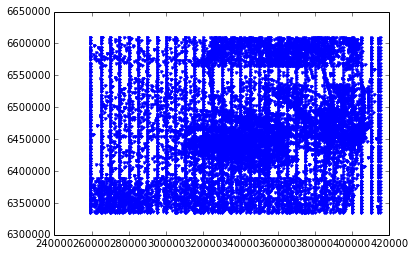
\includegraphics{3D-Structural-Data_6_0.png}

Or, a bit more complex plotting options:

\begin{Verbatim}[commandchars=\\\{\}]
\PYG{n}{fig} \PYG{o}{=} \PYG{n}{plt}\PYG{o}{.}\PYG{n}{figure}\PYG{p}{(}\PYG{n}{figsize} \PYG{o}{=} \PYG{p}{(}\PYG{l+m+mi}{18}\PYG{p}{,}\PYG{l+m+mi}{6}\PYG{p}{)}\PYG{p}{)}
\PYG{n}{ax1} \PYG{o}{=} \PYG{n}{fig}\PYG{o}{.}\PYG{n}{add\PYGZus{}subplot}\PYG{p}{(}\PYG{l+m+mi}{131}\PYG{p}{)}
\PYG{n}{ax2} \PYG{o}{=} \PYG{n}{fig}\PYG{o}{.}\PYG{n}{add\PYGZus{}subplot}\PYG{p}{(}\PYG{l+m+mi}{132}\PYG{p}{)}
\PYG{n}{ax3} \PYG{o}{=} \PYG{n}{fig}\PYG{o}{.}\PYG{n}{add\PYGZus{}subplot}\PYG{p}{(}\PYG{l+m+mi}{133}\PYG{p}{)}
\PYG{n}{pts}\PYG{o}{.}\PYG{n}{plot\PYGZus{}plane}\PYG{p}{(}\PYG{n}{ax} \PYG{o}{=} \PYG{n}{ax1}\PYG{p}{)}
\PYG{n}{pts}\PYG{o}{.}\PYG{n}{plot\PYGZus{}plane}\PYG{p}{(}\PYG{n}{plane} \PYG{o}{=} \PYG{p}{(}\PYG{l+s}{\PYGZsq{}}\PYG{l+s}{x}\PYG{l+s}{\PYGZsq{}}\PYG{p}{,}\PYG{l+s}{\PYGZsq{}}\PYG{l+s}{z}\PYG{l+s}{\PYGZsq{}}\PYG{p}{)}\PYG{p}{,} \PYG{n}{ax} \PYG{o}{=} \PYG{n}{ax2}\PYG{p}{,} \PYG{n}{color} \PYG{o}{=} \PYG{l+s}{\PYGZsq{}}\PYG{l+s}{k}\PYG{l+s}{\PYGZsq{}}\PYG{p}{)}
\PYG{n}{pts}\PYG{o}{.}\PYG{n}{plot\PYGZus{}plane}\PYG{p}{(}\PYG{n}{plane} \PYG{o}{=} \PYG{p}{(}\PYG{l+s}{\PYGZsq{}}\PYG{l+s}{y}\PYG{l+s}{\PYGZsq{}}\PYG{p}{,}\PYG{l+s}{\PYGZsq{}}\PYG{l+s}{z}\PYG{l+s}{\PYGZsq{}}\PYG{p}{)}\PYG{p}{,} \PYG{n}{ax} \PYG{o}{=} \PYG{n}{ax3}\PYG{p}{,} \PYG{n}{color} \PYG{o}{=} \PYG{l+s}{\PYGZsq{}}\PYG{l+s}{r}\PYG{l+s}{\PYGZsq{}}\PYG{p}{)}
\end{Verbatim}

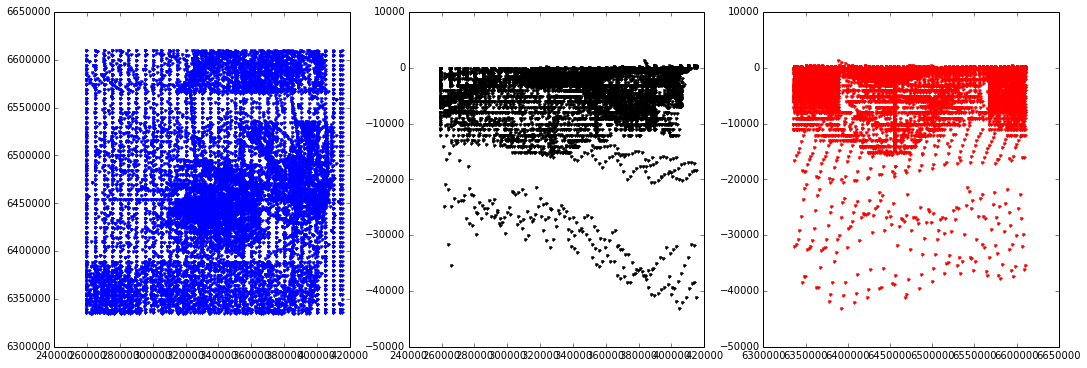
\includegraphics{3D-Structural-Data_8_0.png}

We can also create plots of points for specified formations only:

\begin{Verbatim}[commandchars=\\\{\}]
\PYG{n}{fig} \PYG{o}{=} \PYG{n}{plt}\PYG{o}{.}\PYG{n}{figure}\PYG{p}{(}\PYG{n}{figsize} \PYG{o}{=} \PYG{p}{(}\PYG{l+m+mi}{18}\PYG{p}{,}\PYG{l+m+mi}{6}\PYG{p}{)}\PYG{p}{)}
\PYG{n}{ax1} \PYG{o}{=} \PYG{n}{fig}\PYG{o}{.}\PYG{n}{add\PYGZus{}subplot}\PYG{p}{(}\PYG{l+m+mi}{131}\PYG{p}{)}
\PYG{n}{ax2} \PYG{o}{=} \PYG{n}{fig}\PYG{o}{.}\PYG{n}{add\PYGZus{}subplot}\PYG{p}{(}\PYG{l+m+mi}{132}\PYG{p}{)}
\PYG{n}{ax3} \PYG{o}{=} \PYG{n}{fig}\PYG{o}{.}\PYG{n}{add\PYGZus{}subplot}\PYG{p}{(}\PYG{l+m+mi}{133}\PYG{p}{)}
\PYG{n}{pts}\PYG{o}{.}\PYG{n}{plot\PYGZus{}plane}\PYG{p}{(}\PYG{n}{ax} \PYG{o}{=} \PYG{n}{ax1}\PYG{p}{,} \PYG{n}{formation\PYGZus{}names} \PYG{o}{=} \PYG{p}{[}\PYG{l+s}{\PYGZsq{}}\PYG{l+s}{Basement}\PYG{l+s}{\PYGZsq{}}\PYG{p}{]}\PYG{p}{)}
\PYG{n}{pts}\PYG{o}{.}\PYG{n}{plot\PYGZus{}plane}\PYG{p}{(}\PYG{n}{ax} \PYG{o}{=} \PYG{n}{ax2}\PYG{p}{,} \PYG{n}{formation\PYGZus{}names} \PYG{o}{=} \PYG{p}{[}\PYG{l+s}{\PYGZsq{}}\PYG{l+s}{Yarragadee\PYGZus{}Fm}\PYG{l+s}{\PYGZsq{}}\PYG{p}{]}\PYG{p}{,} \PYG{n}{color} \PYG{o}{=} \PYG{l+s}{\PYGZsq{}}\PYG{l+s}{k}\PYG{l+s}{\PYGZsq{}}\PYG{p}{)}
\PYG{n}{pts}\PYG{o}{.}\PYG{n}{plot\PYGZus{}plane}\PYG{p}{(}\PYG{n}{ax} \PYG{o}{=} \PYG{n}{ax3}\PYG{p}{,} \PYG{n}{formation\PYGZus{}names} \PYG{o}{=} \PYG{p}{[}\PYG{l+s}{\PYGZsq{}}\PYG{l+s}{Lesueur\PYGZus{}Ss}\PYG{l+s}{\PYGZsq{}}\PYG{p}{]}\PYG{p}{,} \PYG{n}{color} \PYG{o}{=} \PYG{l+s}{\PYGZsq{}}\PYG{l+s}{r}\PYG{l+s}{\PYGZsq{}}\PYG{p}{)}
\end{Verbatim}

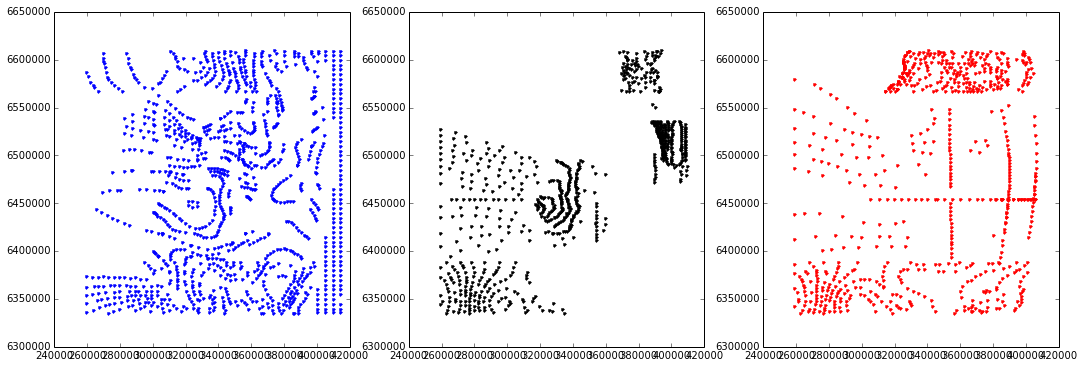
\includegraphics{3D-Structural-Data_10_0.png}

It is also possible to create 3-D perspective plots (not many options
yet, but a lot more could be included):

\begin{Verbatim}[commandchars=\\\{\}]
\PYG{n}{pts}\PYG{o}{.}\PYG{n}{plot\PYGZus{}3D}\PYG{p}{(}\PYG{n}{formation\PYGZus{}names} \PYG{o}{=} \PYG{p}{[}\PYG{l+s}{\PYGZsq{}}\PYG{l+s}{Basement}\PYG{l+s}{\PYGZsq{}}\PYG{p}{]}\PYG{p}{)}
\end{Verbatim}

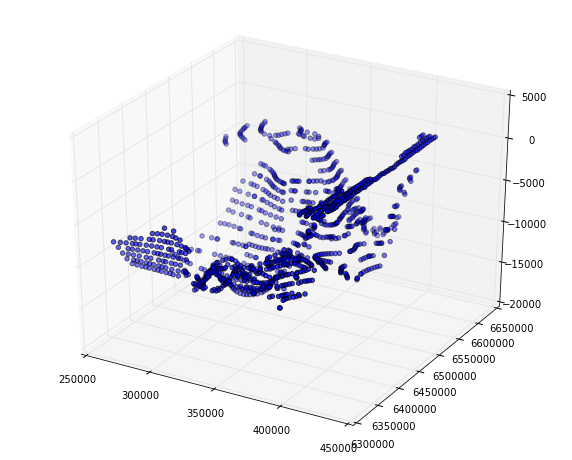
\includegraphics{3D-Structural-Data_12_0.png}

\begin{Verbatim}[commandchars=\\\{\}]
\PYG{n}{pts}\PYG{o}{.}\PYG{n}{formation\PYGZus{}names}
\end{Verbatim}

\begin{Verbatim}[commandchars=\\\{\}]
\PYG{n}{array}\PYG{p}{(}\PYG{p}{[}\PYG{l+s}{\PYGZsq{}}\PYG{l+s}{Basement}\PYG{l+s}{\PYGZsq{}}\PYG{p}{,} \PYG{l+s}{\PYGZsq{}}\PYG{l+s}{CPB\PYGZus{}Fault\PYGZus{}01}\PYG{l+s}{\PYGZsq{}}\PYG{p}{,} \PYG{l+s}{\PYGZsq{}}\PYG{l+s}{CPB\PYGZus{}Fault\PYGZus{}02}\PYG{l+s}{\PYGZsq{}}\PYG{p}{,} \PYG{l+s}{\PYGZsq{}}\PYG{l+s}{CPB\PYGZus{}Fault\PYGZus{}03}\PYG{l+s}{\PYGZsq{}}\PYG{p}{,}
       \PYG{l+s}{\PYGZsq{}}\PYG{l+s}{CPB\PYGZus{}Fault\PYGZus{}04}\PYG{l+s}{\PYGZsq{}}\PYG{p}{,} \PYG{l+s}{\PYGZsq{}}\PYG{l+s}{CPB\PYGZus{}Fault\PYGZus{}05}\PYG{l+s}{\PYGZsq{}}\PYG{p}{,} \PYG{l+s}{\PYGZsq{}}\PYG{l+s}{CPB\PYGZus{}Fault\PYGZus{}06}\PYG{l+s}{\PYGZsq{}}\PYG{p}{,} \PYG{l+s}{\PYGZsq{}}\PYG{l+s}{CPB\PYGZus{}Fault\PYGZus{}07}\PYG{l+s}{\PYGZsq{}}\PYG{p}{,}
       \PYG{l+s}{\PYGZsq{}}\PYG{l+s}{CPB\PYGZus{}Fault\PYGZus{}08}\PYG{l+s}{\PYGZsq{}}\PYG{p}{,} \PYG{l+s}{\PYGZsq{}}\PYG{l+s}{CPB\PYGZus{}Fault\PYGZus{}09}\PYG{l+s}{\PYGZsq{}}\PYG{p}{,} \PYG{l+s}{\PYGZsq{}}\PYG{l+s}{CPB\PYGZus{}Fault\PYGZus{}10}\PYG{l+s}{\PYGZsq{}}\PYG{p}{,}
       \PYG{l+s}{\PYGZsq{}}\PYG{l+s}{CPB\PYGZus{}Fault\PYGZus{}11\PYGZus{}Serpentine}\PYG{l+s}{\PYGZsq{}}\PYG{p}{,} \PYG{l+s}{\PYGZsq{}}\PYG{l+s}{CPB\PYGZus{}Fault\PYGZus{}12\PYGZus{}Darling}\PYG{l+s}{\PYGZsq{}}\PYG{p}{,} \PYG{l+s}{\PYGZsq{}}\PYG{l+s}{CPB\PYGZus{}Fault\PYGZus{}13}\PYG{l+s}{\PYGZsq{}}\PYG{p}{,}
       \PYG{l+s}{\PYGZsq{}}\PYG{l+s}{CPB\PYGZus{}Fault\PYGZus{}14}\PYG{l+s}{\PYGZsq{}}\PYG{p}{,} \PYG{l+s}{\PYGZsq{}}\PYG{l+s}{CPB\PYGZus{}Fault\PYGZus{}15}\PYG{l+s}{\PYGZsq{}}\PYG{p}{,} \PYG{l+s}{\PYGZsq{}}\PYG{l+s}{CPB\PYGZus{}Fault\PYGZus{}16}\PYG{l+s}{\PYGZsq{}}\PYG{p}{,}
       \PYG{l+s}{\PYGZsq{}}\PYG{l+s}{CPB\PYGZus{}Fault\PYGZus{}Transverse\PYGZus{}02}\PYG{l+s}{\PYGZsq{}}\PYG{p}{,} \PYG{l+s}{\PYGZsq{}}\PYG{l+s}{CPB\PYGZus{}Fault\PYGZus{}Transverse\PYGZus{}03}\PYG{l+s}{\PYGZsq{}}\PYG{p}{,}
       \PYG{l+s}{\PYGZsq{}}\PYG{l+s}{CPB\PYGZus{}Fault\PYGZus{}Transverse\PYGZus{}04}\PYG{l+s}{\PYGZsq{}}\PYG{p}{,} \PYG{l+s}{\PYGZsq{}}\PYG{l+s}{CPB\PYGZus{}Fault\PYGZus{}Transverse\PYGZus{}05}\PYG{l+s}{\PYGZsq{}}\PYG{p}{,}
       \PYG{l+s}{\PYGZsq{}}\PYG{l+s}{Cattamarra\PYGZus{}Coal\PYGZus{}Measures}\PYG{l+s}{\PYGZsq{}}\PYG{p}{,} \PYG{l+s}{\PYGZsq{}}\PYG{l+s}{Eneabba\PYGZus{}Fm}\PYG{l+s}{\PYGZsq{}}\PYG{p}{,} \PYG{l+s}{\PYGZsq{}}\PYG{l+s}{Gage\PYGZus{}Ss}\PYG{l+s}{\PYGZsq{}}\PYG{p}{,}
       \PYG{l+s}{\PYGZsq{}}\PYG{l+s}{Kockatea\PYGZus{}Shale}\PYG{l+s}{\PYGZsq{}}\PYG{p}{,} \PYG{l+s}{\PYGZsq{}}\PYG{l+s}{Late\PYGZus{}Triassic}\PYG{l+s}{\PYGZsq{}}\PYG{p}{,} \PYG{l+s}{\PYGZsq{}}\PYG{l+s}{Leederville\PYGZus{}Fm}\PYG{l+s}{\PYGZsq{}}\PYG{p}{,} \PYG{l+s}{\PYGZsq{}}\PYG{l+s}{Lesueur\PYGZus{}Ss}\PYG{l+s}{\PYGZsq{}}\PYG{p}{,}
       \PYG{l+s}{\PYGZsq{}}\PYG{l+s}{Lower\PYGZus{}crust}\PYG{l+s}{\PYGZsq{}}\PYG{p}{,} \PYG{l+s}{\PYGZsq{}}\PYG{l+s}{Moho}\PYG{l+s}{\PYGZsq{}}\PYG{p}{,} \PYG{l+s}{\PYGZsq{}}\PYG{l+s}{Neocomian\PYGZus{}Unc}\PYG{l+s}{\PYGZsq{}}\PYG{p}{,} \PYG{l+s}{\PYGZsq{}}\PYG{l+s}{Permian}\PYG{l+s}{\PYGZsq{}}\PYG{p}{,} \PYG{l+s}{\PYGZsq{}}\PYG{l+s}{Sea\PYGZus{}level}\PYG{l+s}{\PYGZsq{}}\PYG{p}{,}
       \PYG{l+s}{\PYGZsq{}}\PYG{l+s}{South\PYGZus{}Perth\PYGZus{}Sh}\PYG{l+s}{\PYGZsq{}}\PYG{p}{,} \PYG{l+s}{\PYGZsq{}}\PYG{l+s}{Topo}\PYG{l+s}{\PYGZsq{}}\PYG{p}{,} \PYG{l+s}{\PYGZsq{}}\PYG{l+s}{Yarragadee\PYGZus{}Fm}\PYG{l+s}{\PYGZsq{}}\PYG{p}{,} \PYG{l+s}{\PYGZsq{}}\PYG{l+s}{Yilgarn}\PYG{l+s}{\PYGZsq{}}\PYG{p}{]}\PYG{p}{,}
      \PYG{n}{dtype}\PYG{o}{=}\PYG{l+s}{\PYGZsq{}}\PYG{l+s}{\textbar{}S32}\PYG{l+s}{\PYGZsq{}}\PYG{p}{)}
\end{Verbatim}

Generate subset for defined formations

It is often required to generate a subset of the points, either for
specified formations only (although that could also be done during the
input in GeoModeller...), or for a defined range/ extent. These options
are possible with the package, and selections can be stored to new
files:

\begin{Verbatim}[commandchars=\\\{\}]
\PYG{c}{\PYGZsh{} only required during testing stage}
\PYG{n+nb}{reload}\PYG{p}{(}\PYG{n}{struct\PYGZus{}data}\PYG{p}{)}
\PYG{c}{\PYGZsh{} use example data}
\PYG{n}{pts} \PYG{o}{=} \PYG{n}{struct\PYGZus{}data}\PYG{o}{.}\PYG{n}{Struct3DPoints}\PYG{p}{(}\PYG{n}{filename} \PYG{o}{=} \PYG{l+s}{r\PYGZsq{}}\PYG{l+s}{../data/wt\PYGZus{}Points.csv}\PYG{l+s}{\PYGZsq{}}\PYG{p}{)}
\PYG{n}{pts\PYGZus{}subset} \PYG{o}{=} \PYG{n}{pts}\PYG{o}{.}\PYG{n}{create\PYGZus{}formation\PYGZus{}subset}\PYG{p}{(}\PYG{p}{[}\PYG{l+s}{\PYGZsq{}}\PYG{l+s}{Basement}\PYG{l+s}{\PYGZsq{}}\PYG{p}{]}\PYG{p}{)}
\end{Verbatim}

\begin{Verbatim}[commandchars=\\\{\}]
\PYG{n}{pts\PYGZus{}subset}\PYG{o}{.}\PYG{n}{len}
\end{Verbatim}

\begin{Verbatim}[commandchars=\\\{\}]
\PYG{l+m+mi}{1209}
\end{Verbatim}

\begin{Verbatim}[commandchars=\\\{\}]
\PYG{n}{pts\PYGZus{}subset}\PYG{o}{.}\PYG{n}{plot\PYGZus{}3D}\PYG{p}{(}\PYG{p}{)}
\end{Verbatim}

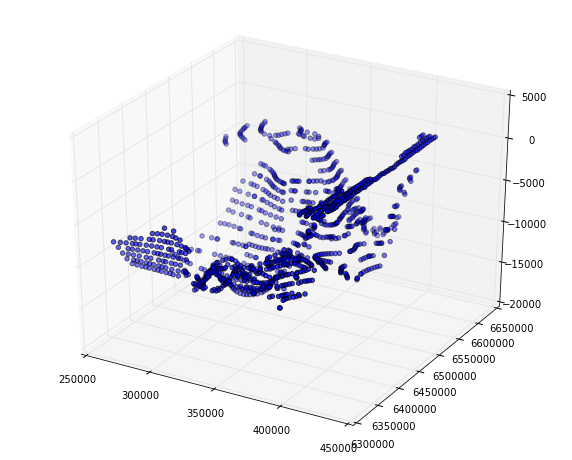
\includegraphics{3D-Structural-Data_17_0.png}

Generating a subset for a subvolume

It is also possible to extract data in only a specified range. The range
is defined with keywords, e.g. \code{from\_x = xx}, \code{to\_x = xx}. All other
ranges (not stated) are simply kept as before.

Here an example:

\begin{Verbatim}[commandchars=\\\{\}]
\PYG{c}{\PYGZsh{} only required during testing stage}
\PYG{n+nb}{reload}\PYG{p}{(}\PYG{n}{struct\PYGZus{}data}\PYG{p}{)}
\PYG{c}{\PYGZsh{} use example data}
\PYG{n}{pts} \PYG{o}{=} \PYG{n}{struct\PYGZus{}data}\PYG{o}{.}\PYG{n}{Struct3DPoints}\PYG{p}{(}\PYG{n}{filename} \PYG{o}{=} \PYG{l+s}{r\PYGZsq{}}\PYG{l+s}{../data/wt\PYGZus{}Points.csv}\PYG{l+s}{\PYGZsq{}}\PYG{p}{)}
\end{Verbatim}

\begin{Verbatim}[commandchars=\\\{\}]
\PYG{n}{pts}\PYG{o}{.}\PYG{n}{xmin}\PYG{p}{,} \PYG{n}{pts}\PYG{o}{.}\PYG{n}{xmax}\PYG{p}{,} \PYG{n}{pts}\PYG{o}{.}\PYG{n}{ymin}\PYG{p}{,} \PYG{n}{pts}\PYG{o}{.}\PYG{n}{ymax}
\end{Verbatim}

\begin{Verbatim}[commandchars=\\\{\}]
\PYG{p}{(}\PYG{l+m+mf}{259000.0}\PYG{p}{,} \PYG{l+m+mf}{415000.0}\PYG{p}{,} \PYG{l+m+mf}{6335020.0}\PYG{p}{,} \PYG{l+m+mf}{6610000.0}\PYG{p}{)}
\end{Verbatim}

\begin{Verbatim}[commandchars=\\\{\}]
\PYG{n}{pts\PYGZus{}subset} \PYG{o}{=} \PYG{n}{pts}\PYG{o}{.}\PYG{n}{extract\PYGZus{}range}\PYG{p}{(}\PYG{n}{from\PYGZus{}x} \PYG{o}{=} \PYG{l+m+mf}{350000.}\PYG{p}{,} \PYG{n}{to\PYGZus{}y} \PYG{o}{=} \PYG{l+m+mi}{6500000}\PYG{p}{)}
\end{Verbatim}

Now let's compare the two sets in a plot:

\begin{Verbatim}[commandchars=\\\{\}]
\PYG{n}{fig} \PYG{o}{=} \PYG{n}{plt}\PYG{o}{.}\PYG{n}{figure}\PYG{p}{(}\PYG{n}{figsize} \PYG{o}{=} \PYG{p}{(}\PYG{l+m+mi}{15}\PYG{p}{,}\PYG{l+m+mi}{6}\PYG{p}{)}\PYG{p}{)}
\PYG{n}{ax1} \PYG{o}{=} \PYG{n}{fig}\PYG{o}{.}\PYG{n}{add\PYGZus{}subplot}\PYG{p}{(}\PYG{l+m+mi}{121}\PYG{p}{)}
\PYG{n}{ax2} \PYG{o}{=} \PYG{n}{fig}\PYG{o}{.}\PYG{n}{add\PYGZus{}subplot}\PYG{p}{(}\PYG{l+m+mi}{122}\PYG{p}{)}
\PYG{n}{pts}\PYG{o}{.}\PYG{n}{plot\PYGZus{}plane}\PYG{p}{(}\PYG{n}{ax} \PYG{o}{=} \PYG{n}{ax1}\PYG{p}{,} \PYG{n}{formation\PYGZus{}names} \PYG{o}{=} \PYG{p}{[}\PYG{l+s}{\PYGZsq{}}\PYG{l+s}{Basement}\PYG{l+s}{\PYGZsq{}}\PYG{p}{]}\PYG{p}{)}
\PYG{n}{pts\PYGZus{}subset}\PYG{o}{.}\PYG{n}{plot\PYGZus{}plane}\PYG{p}{(}\PYG{n}{ax} \PYG{o}{=} \PYG{n}{ax2}\PYG{p}{,} \PYG{n}{formation\PYGZus{}names} \PYG{o}{=} \PYG{p}{[}\PYG{l+s}{\PYGZsq{}}\PYG{l+s}{Basement}\PYG{l+s}{\PYGZsq{}}\PYG{p}{]}\PYG{p}{)}
\PYG{c}{\PYGZsh{} set ranges to compare plots}
\PYG{n}{ax1}\PYG{o}{.}\PYG{n}{set\PYGZus{}xlim}\PYG{p}{(}\PYG{p}{(}\PYG{n}{pts}\PYG{o}{.}\PYG{n}{xmin}\PYG{o}{\PYGZhy{}}\PYG{l+m+mi}{10000}\PYG{p}{,} \PYG{n}{pts}\PYG{o}{.}\PYG{n}{xmax}\PYG{o}{+}\PYG{l+m+mi}{10000}\PYG{p}{)}\PYG{p}{)}
\PYG{n}{ax1}\PYG{o}{.}\PYG{n}{set\PYGZus{}ylim}\PYG{p}{(}\PYG{p}{(}\PYG{n}{pts}\PYG{o}{.}\PYG{n}{ymin}\PYG{o}{\PYGZhy{}}\PYG{l+m+mi}{10000}\PYG{p}{,} \PYG{n}{pts}\PYG{o}{.}\PYG{n}{ymax}\PYG{o}{+}\PYG{l+m+mi}{10000}\PYG{p}{)}\PYG{p}{)}
\PYG{n}{ax2}\PYG{o}{.}\PYG{n}{set\PYGZus{}xlim}\PYG{p}{(}\PYG{p}{(}\PYG{n}{pts}\PYG{o}{.}\PYG{n}{xmin}\PYG{o}{\PYGZhy{}}\PYG{l+m+mi}{10000}\PYG{p}{,} \PYG{n}{pts}\PYG{o}{.}\PYG{n}{xmax}\PYG{o}{+}\PYG{l+m+mi}{10000}\PYG{p}{)}\PYG{p}{)}
\PYG{n}{ax2}\PYG{o}{.}\PYG{n}{set\PYGZus{}ylim}\PYG{p}{(}\PYG{p}{(}\PYG{n}{pts}\PYG{o}{.}\PYG{n}{ymin}\PYG{o}{\PYGZhy{}}\PYG{l+m+mi}{10000}\PYG{p}{,} \PYG{n}{pts}\PYG{o}{.}\PYG{n}{ymax}\PYG{o}{+}\PYG{l+m+mi}{10000}\PYG{p}{)}\PYG{p}{)}
\end{Verbatim}

\begin{Verbatim}[commandchars=\\\{\}]
\PYG{p}{(}\PYG{l+m+mf}{6325020.0}\PYG{p}{,} \PYG{l+m+mf}{6620000.0}\PYG{p}{)}
\end{Verbatim}

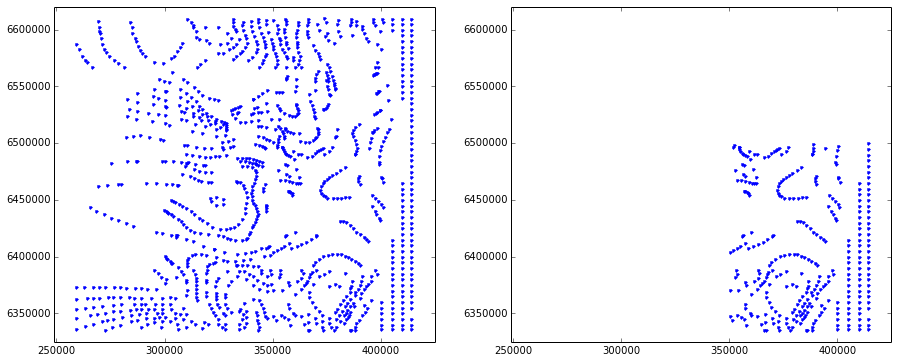
\includegraphics{3D-Structural-Data_23_1.png}

Thin data

In many cases, a lot of data has been digitised for specific locations.
This can lead to problems with the kriging interpolation in Geomodeller.
A simple function to thin data is implemented here to avoid this
problem. The method is really simple and can be quite compute intense
(for smalll grids), so check what you are doing!

Note: If spatial data is imported, Geomodeller actually has a
functionality for a type of ``thinning'' - if you work with this data
(e.g. digitised from MapInfo), then this might be the function to use...

The thinning is performed for \textbf{the entire set} and \textbf{not aware of
formations} (so far...) and works on a grid/ raster base for defined
number of cells in each axis direction of \code{nx, ny, nz}. The best
procedure is therefore to first create a subset for one formation, and
then to perform the thinning for this subset:

\begin{Verbatim}[commandchars=\\\{\}]
\PYG{c}{\PYGZsh{} only required during testing stage}
\PYG{n+nb}{reload}\PYG{p}{(}\PYG{n}{struct\PYGZus{}data}\PYG{p}{)}
\PYG{c}{\PYGZsh{} use example data}
\PYG{n}{pts} \PYG{o}{=} \PYG{n}{struct\PYGZus{}data}\PYG{o}{.}\PYG{n}{Struct3DPoints}\PYG{p}{(}\PYG{n}{filename} \PYG{o}{=} \PYG{l+s}{r\PYGZsq{}}\PYG{l+s}{../data/wt\PYGZus{}Points.csv}\PYG{l+s}{\PYGZsq{}}\PYG{p}{)}
\PYG{n}{pts\PYGZus{}sub1} \PYG{o}{=} \PYG{n}{pts}\PYG{o}{.}\PYG{n}{create\PYGZus{}formation\PYGZus{}subset}\PYG{p}{(}\PYG{l+s}{\PYGZsq{}}\PYG{l+s}{Permian}\PYG{l+s}{\PYGZsq{}}\PYG{p}{)}
\end{Verbatim}

Let's have a look at one formation, the Permian. We can clearly see the
dense data in the overlapping regions and the highly defined traces
through the model:

\begin{Verbatim}[commandchars=\\\{\}]
\PYG{n}{fig} \PYG{o}{=} \PYG{n}{plt}\PYG{o}{.}\PYG{n}{figure}\PYG{p}{(}\PYG{n}{figsize} \PYG{o}{=} \PYG{p}{(}\PYG{l+m+mi}{16}\PYG{p}{,}\PYG{l+m+mi}{6}\PYG{p}{)}\PYG{p}{)}
\PYG{n}{ax1} \PYG{o}{=} \PYG{n}{fig}\PYG{o}{.}\PYG{n}{add\PYGZus{}subplot}\PYG{p}{(}\PYG{l+m+mi}{121}\PYG{p}{,} \PYG{n}{projection}\PYG{o}{=}\PYG{l+s}{\PYGZsq{}}\PYG{l+s}{3d}\PYG{l+s}{\PYGZsq{}}\PYG{p}{)}
\PYG{n}{ax2} \PYG{o}{=} \PYG{n}{fig}\PYG{o}{.}\PYG{n}{add\PYGZus{}subplot}\PYG{p}{(}\PYG{l+m+mi}{122}\PYG{p}{)}
\PYG{n}{ax1}\PYG{o}{.}\PYG{n}{view\PYGZus{}init}\PYG{p}{(}\PYG{n}{elev}\PYG{o}{=}\PYG{l+m+mi}{30}\PYG{p}{,} \PYG{n}{azim}\PYG{o}{=}\PYG{l+m+mi}{70}\PYG{p}{)}
\PYG{n}{pts\PYGZus{}sub1}\PYG{o}{.}\PYG{n}{plot\PYGZus{}3D}\PYG{p}{(}\PYG{n}{ax} \PYG{o}{=} \PYG{n}{ax1}\PYG{p}{)}
\PYG{n}{pts\PYGZus{}sub1}\PYG{o}{.}\PYG{n}{plot\PYGZus{}plane}\PYG{p}{(}\PYG{n}{ax} \PYG{o}{=} \PYG{n}{ax2}\PYG{p}{)}
\end{Verbatim}

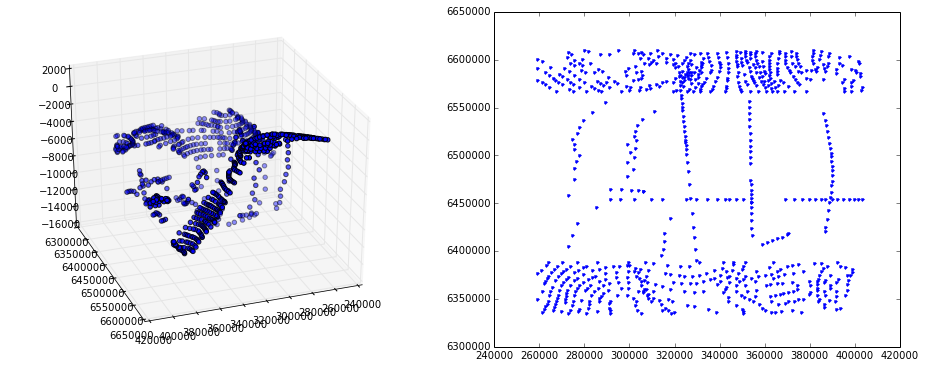
\includegraphics{3D-Structural-Data_27_0.png}

We want to thin this now with a grid which is \code{n} times smaller than
the extent in each direction:

\begin{Verbatim}[commandchars=\\\{\}]
\PYG{n}{nx} \PYG{o}{=} \PYG{l+m+mi}{20}
\PYG{n}{ny} \PYG{o}{=} \PYG{l+m+mi}{20}
\PYG{n}{nz} \PYG{o}{=} \PYG{l+m+mi}{20}

\PYG{n}{pts\PYGZus{}sub2} \PYG{o}{=} \PYG{n}{pts\PYGZus{}sub1}\PYG{o}{.}\PYG{n}{thin}\PYG{p}{(}\PYG{n}{nx}\PYG{p}{,} \PYG{n}{ny}\PYG{p}{,} \PYG{n}{nz}\PYG{p}{)}
\end{Verbatim}

\begin{Verbatim}[commandchars=\\\{\}]
\PYG{n}{pts\PYGZus{}sub1}\PYG{o}{.}\PYG{n}{len}\PYG{p}{,} \PYG{n}{pts\PYGZus{}sub2}\PYG{o}{.}\PYG{n}{len}
\end{Verbatim}

\begin{Verbatim}[commandchars=\\\{\}]
\PYG{p}{(}\PYG{l+m+mi}{810}\PYG{p}{,} \PYG{l+m+mi}{319}\PYG{p}{)}
\end{Verbatim}

And compare those to the set above in a plot:

\begin{Verbatim}[commandchars=\\\{\}]
\PYG{n}{fig} \PYG{o}{=} \PYG{n}{plt}\PYG{o}{.}\PYG{n}{figure}\PYG{p}{(}\PYG{n}{figsize} \PYG{o}{=} \PYG{p}{(}\PYG{l+m+mi}{16}\PYG{p}{,}\PYG{l+m+mi}{6}\PYG{p}{)}\PYG{p}{)}
\PYG{n}{ax1} \PYG{o}{=} \PYG{n}{fig}\PYG{o}{.}\PYG{n}{add\PYGZus{}subplot}\PYG{p}{(}\PYG{l+m+mi}{121}\PYG{p}{,} \PYG{n}{projection}\PYG{o}{=}\PYG{l+s}{\PYGZsq{}}\PYG{l+s}{3d}\PYG{l+s}{\PYGZsq{}}\PYG{p}{)}
\PYG{n}{ax2} \PYG{o}{=} \PYG{n}{fig}\PYG{o}{.}\PYG{n}{add\PYGZus{}subplot}\PYG{p}{(}\PYG{l+m+mi}{122}\PYG{p}{)}
\PYG{n}{ax1}\PYG{o}{.}\PYG{n}{view\PYGZus{}init}\PYG{p}{(}\PYG{n}{elev}\PYG{o}{=}\PYG{l+m+mi}{30}\PYG{p}{,} \PYG{n}{azim}\PYG{o}{=}\PYG{l+m+mi}{70}\PYG{p}{)}
\PYG{n}{pts\PYGZus{}sub2}\PYG{o}{.}\PYG{n}{plot\PYGZus{}3D}\PYG{p}{(}\PYG{n}{ax} \PYG{o}{=} \PYG{n}{ax1}\PYG{p}{)}
\PYG{n}{pts\PYGZus{}sub2}\PYG{o}{.}\PYG{n}{plot\PYGZus{}plane}\PYG{p}{(}\PYG{n}{ax} \PYG{o}{=} \PYG{n}{ax2}\PYG{p}{)}
\end{Verbatim}

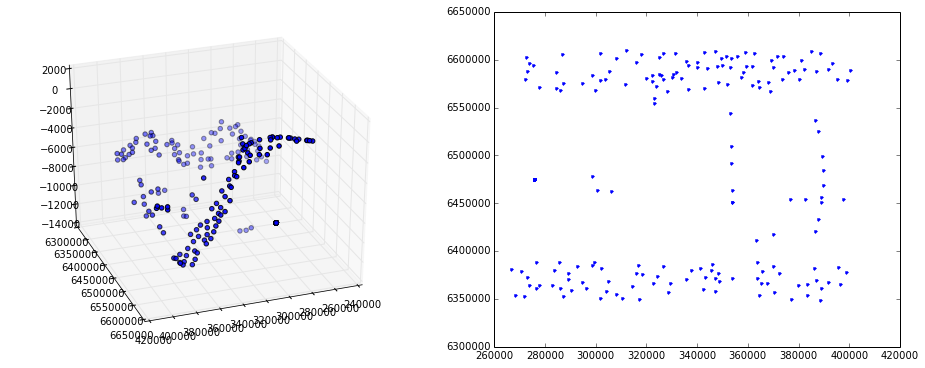
\includegraphics{3D-Structural-Data_32_0.png}

Nice, it seems to work (surprised myself...)

Of course, it's up to the user to evaluate if the thinning is creating
``wrong'' Geomodels afterwards... good luck!

Combine two point sets

It might be important to combine datasets, for example after thinning
two different geological formations. As an example, we will combine the
thinned Permian data set from above with the (complete) set for the
Basement:

\begin{Verbatim}[commandchars=\\\{\}]
\PYG{c}{\PYGZsh{} only required during testing stage}
\PYG{n+nb}{reload}\PYG{p}{(}\PYG{n}{struct\PYGZus{}data}\PYG{p}{)}
\PYG{c}{\PYGZsh{} use example data}
\PYG{n}{pts} \PYG{o}{=} \PYG{n}{struct\PYGZus{}data}\PYG{o}{.}\PYG{n}{Struct3DPoints}\PYG{p}{(}\PYG{n}{filename} \PYG{o}{=} \PYG{l+s}{r\PYGZsq{}}\PYG{l+s}{../data/wt\PYGZus{}Points.csv}\PYG{l+s}{\PYGZsq{}}\PYG{p}{)}
\PYG{n}{pts\PYGZus{}sub3} \PYG{o}{=} \PYG{n}{pts}\PYG{o}{.}\PYG{n}{create\PYGZus{}formation\PYGZus{}subset}\PYG{p}{(}\PYG{l+s}{\PYGZsq{}}\PYG{l+s}{Basement}\PYG{l+s}{\PYGZsq{}}\PYG{p}{)}
\PYG{c}{\PYGZsh{} create a copy for comparison:}
\PYG{n}{pts\PYGZus{}sub3b} \PYG{o}{=} \PYG{n}{pts}\PYG{o}{.}\PYG{n}{create\PYGZus{}formation\PYGZus{}subset}\PYG{p}{(}\PYG{l+s}{\PYGZsq{}}\PYG{l+s}{Basement}\PYG{l+s}{\PYGZsq{}}\PYG{p}{)}

\PYG{n}{pts\PYGZus{}sub3}\PYG{o}{.}\PYG{n}{combine\PYGZus{}with}\PYG{p}{(}\PYG{n}{pts\PYGZus{}sub2}\PYG{p}{)}

\PYG{c}{\PYGZsh{} create a plot of all three point sets:}
\PYG{n}{fig} \PYG{o}{=} \PYG{n}{plt}\PYG{o}{.}\PYG{n}{figure}\PYG{p}{(}\PYG{n}{figsize} \PYG{o}{=} \PYG{p}{(}\PYG{l+m+mi}{18}\PYG{p}{,}\PYG{l+m+mi}{6}\PYG{p}{)}\PYG{p}{)}
\PYG{n}{ax1} \PYG{o}{=} \PYG{n}{fig}\PYG{o}{.}\PYG{n}{add\PYGZus{}subplot}\PYG{p}{(}\PYG{l+m+mi}{131}\PYG{p}{)}
\PYG{n}{ax2} \PYG{o}{=} \PYG{n}{fig}\PYG{o}{.}\PYG{n}{add\PYGZus{}subplot}\PYG{p}{(}\PYG{l+m+mi}{132}\PYG{p}{)}
\PYG{n}{ax3} \PYG{o}{=} \PYG{n}{fig}\PYG{o}{.}\PYG{n}{add\PYGZus{}subplot}\PYG{p}{(}\PYG{l+m+mi}{133}\PYG{p}{)}
\PYG{n}{pts\PYGZus{}sub3b}\PYG{o}{.}\PYG{n}{plot\PYGZus{}plane}\PYG{p}{(}\PYG{p}{(}\PYG{l+s}{\PYGZsq{}}\PYG{l+s}{x}\PYG{l+s}{\PYGZsq{}}\PYG{p}{,}\PYG{l+s}{\PYGZsq{}}\PYG{l+s}{z}\PYG{l+s}{\PYGZsq{}}\PYG{p}{)}\PYG{p}{,} \PYG{n}{ax} \PYG{o}{=} \PYG{n}{ax1}\PYG{p}{)}
\PYG{n}{pts\PYGZus{}sub2}\PYG{o}{.}\PYG{n}{plot\PYGZus{}plane}\PYG{p}{(}\PYG{p}{(}\PYG{l+s}{\PYGZsq{}}\PYG{l+s}{x}\PYG{l+s}{\PYGZsq{}}\PYG{p}{,}\PYG{l+s}{\PYGZsq{}}\PYG{l+s}{z}\PYG{l+s}{\PYGZsq{}}\PYG{p}{)}\PYG{p}{,} \PYG{n}{ax} \PYG{o}{=} \PYG{n}{ax2}\PYG{p}{,} \PYG{n}{color}\PYG{o}{=}\PYG{l+s}{\PYGZsq{}}\PYG{l+s}{r}\PYG{l+s}{\PYGZsq{}}\PYG{p}{)}
\PYG{n}{pts\PYGZus{}sub3}\PYG{o}{.}\PYG{n}{plot\PYGZus{}plane}\PYG{p}{(}\PYG{p}{(}\PYG{l+s}{\PYGZsq{}}\PYG{l+s}{x}\PYG{l+s}{\PYGZsq{}}\PYG{p}{,}\PYG{l+s}{\PYGZsq{}}\PYG{l+s}{z}\PYG{l+s}{\PYGZsq{}}\PYG{p}{)}\PYG{p}{,} \PYG{n}{ax} \PYG{o}{=} \PYG{n}{ax3}\PYG{p}{)}
\PYG{n}{ax1}\PYG{o}{.}\PYG{n}{set\PYGZus{}ylim}\PYG{p}{(}\PYG{p}{(}\PYG{n}{pts\PYGZus{}sub3}\PYG{o}{.}\PYG{n}{zmin}\PYG{p}{,} \PYG{n}{pts\PYGZus{}sub3}\PYG{o}{.}\PYG{n}{zmax}\PYG{p}{)}\PYG{p}{)}
\PYG{n}{ax2}\PYG{o}{.}\PYG{n}{set\PYGZus{}ylim}\PYG{p}{(}\PYG{p}{(}\PYG{n}{pts\PYGZus{}sub3}\PYG{o}{.}\PYG{n}{zmin}\PYG{p}{,} \PYG{n}{pts\PYGZus{}sub3}\PYG{o}{.}\PYG{n}{zmax}\PYG{p}{)}\PYG{p}{)}
\PYG{n}{ax3}\PYG{o}{.}\PYG{n}{set\PYGZus{}ylim}\PYG{p}{(}\PYG{p}{(}\PYG{n}{pts\PYGZus{}sub3}\PYG{o}{.}\PYG{n}{zmin}\PYG{p}{,} \PYG{n}{pts\PYGZus{}sub3}\PYG{o}{.}\PYG{n}{zmax}\PYG{p}{)}\PYG{p}{)}
\end{Verbatim}

\begin{Verbatim}[commandchars=\\\{\}]
\PYG{p}{(}\PYG{o}{\PYGZhy{}}\PYG{l+m+mf}{15400.0}\PYG{p}{,} \PYG{l+m+mf}{454.0}\PYG{p}{)}
\end{Verbatim}

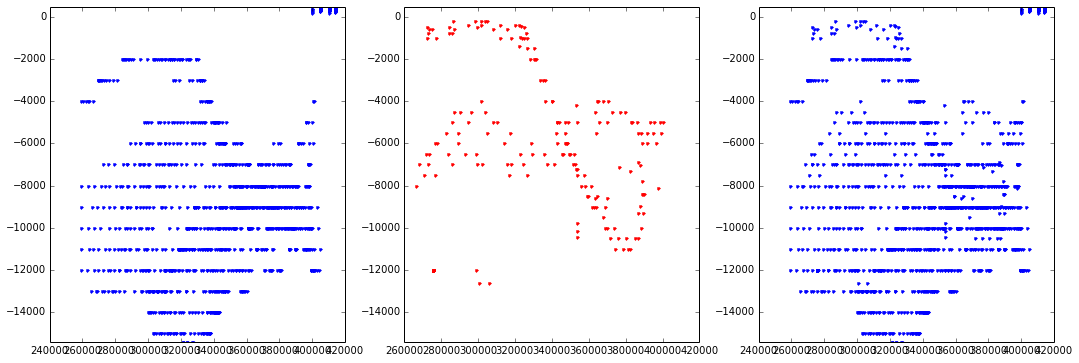
\includegraphics{3D-Structural-Data_35_1.png}

\textbf{Note}: This function changes the pointset in place and does not
return a new one (as for thinning, subsetting, etc.)

Remove formation from point set

It is also possible to remove one or multiple formations from the set.
This functionality can be used in combination with thinning and
combining to thin only the data set for one formation, and then combine
it back into the original set:

\begin{Verbatim}[commandchars=\\\{\}]
\PYG{c}{\PYGZsh{} only required during testing stage}
\PYG{n+nb}{reload}\PYG{p}{(}\PYG{n}{struct\PYGZus{}data}\PYG{p}{)}
\PYG{c}{\PYGZsh{} use example data}
\PYG{n}{pts} \PYG{o}{=} \PYG{n}{struct\PYGZus{}data}\PYG{o}{.}\PYG{n}{Struct3DPoints}\PYG{p}{(}\PYG{n}{filename} \PYG{o}{=} \PYG{l+s}{r\PYGZsq{}}\PYG{l+s}{../data/wt\PYGZus{}Points.csv}\PYG{l+s}{\PYGZsq{}}\PYG{p}{)}

\PYG{k}{print}\PYG{p}{(}\PYG{l+s}{\PYGZdq{}}\PYG{l+s}{Original length of point set: }\PYG{l+s+si}{\PYGZpc{}d}\PYG{l+s}{\PYGZdq{}} \PYG{o}{\PYGZpc{}} \PYG{n}{pts}\PYG{o}{.}\PYG{n}{len}\PYG{p}{)}


\PYG{c}{\PYGZsh{} formation to perform thinning:}
\PYG{n}{formation} \PYG{o}{=} \PYG{l+s}{\PYGZsq{}}\PYG{l+s}{Permian}\PYG{l+s}{\PYGZsq{}}

\PYG{c}{\PYGZsh{} first step: extract formation}
\PYG{n}{pts\PYGZus{}perm} \PYG{o}{=} \PYG{n}{pts}\PYG{o}{.}\PYG{n}{create\PYGZus{}formation\PYGZus{}subset}\PYG{p}{(}\PYG{n}{formation}\PYG{p}{)}

\PYG{c}{\PYGZsh{} now remove from original}
\PYG{n}{pts}\PYG{o}{.}\PYG{n}{remove\PYGZus{}formations}\PYG{p}{(}\PYG{n}{formation}\PYG{p}{)}

\PYG{c}{\PYGZsh{} perform thinning}
\PYG{n}{nx} \PYG{o}{=} \PYG{n}{ny} \PYG{o}{=} \PYG{n}{nz} \PYG{o}{=} \PYG{l+m+mi}{20}
\PYG{n}{pts\PYGZus{}perm\PYGZus{}thinned} \PYG{o}{=} \PYG{n}{pts\PYGZus{}perm}\PYG{o}{.}\PYG{n}{thin}\PYG{p}{(}\PYG{n}{nx}\PYG{p}{,} \PYG{n}{ny}\PYG{p}{,} \PYG{n}{nz}\PYG{p}{)}

\PYG{c}{\PYGZsh{} and now combine back with original:}
\PYG{n}{pts}\PYG{o}{.}\PYG{n}{combine\PYGZus{}with}\PYG{p}{(}\PYG{n}{pts\PYGZus{}perm\PYGZus{}thinned}\PYG{p}{)}

\PYG{k}{print}\PYG{p}{(}\PYG{l+s}{\PYGZdq{}}\PYG{l+s}{New length of point set (after thinning): }\PYG{l+s+si}{\PYGZpc{}d}\PYG{l+s}{\PYGZdq{}} \PYG{o}{\PYGZpc{}} \PYG{n}{pts}\PYG{o}{.}\PYG{n}{len}\PYG{p}{)}
\end{Verbatim}

\begin{Verbatim}[commandchars=\\\{\}]
Original length of point set: 14184
New length of point set (after thinning): 13693
\end{Verbatim}

Save new set to file

Of course, we want to save this new and adapted data set to a file! This
is also simply possible with:

\begin{Verbatim}[commandchars=\\\{\}]
\PYG{c}{\PYGZsh{} only required during testing stage}
\PYG{n+nb}{reload}\PYG{p}{(}\PYG{n}{struct\PYGZus{}data}\PYG{p}{)}
\PYG{c}{\PYGZsh{} use example data}
\PYG{n}{pts} \PYG{o}{=} \PYG{n}{struct\PYGZus{}data}\PYG{o}{.}\PYG{n}{Struct3DPoints}\PYG{p}{(}\PYG{n}{filename} \PYG{o}{=} \PYG{l+s}{r\PYGZsq{}}\PYG{l+s}{../data/wt\PYGZus{}Points.csv}\PYG{l+s}{\PYGZsq{}}\PYG{p}{)}

\PYG{c}{\PYGZsh{} extract defined range and only Basement points:}
\PYG{n}{pts\PYGZus{}subset} \PYG{o}{=} \PYG{n}{pts}\PYG{o}{.}\PYG{n}{create\PYGZus{}formation\PYGZus{}subset}\PYG{p}{(}\PYG{p}{[}\PYG{l+s}{\PYGZsq{}}\PYG{l+s}{Basement}\PYG{l+s}{\PYGZsq{}}\PYG{p}{]}\PYG{p}{)}
\PYG{n}{pts\PYGZus{}subset\PYGZus{}1} \PYG{o}{=} \PYG{n}{pts\PYGZus{}subset}\PYG{o}{.}\PYG{n}{extract\PYGZus{}range}\PYG{p}{(}\PYG{n}{from\PYGZus{}x} \PYG{o}{=} \PYG{l+m+mf}{350000.}\PYG{p}{,} \PYG{n}{to\PYGZus{}y} \PYG{o}{=} \PYG{l+m+mi}{6500000}\PYG{p}{)}

\PYG{n}{pts\PYGZus{}subset\PYGZus{}1}\PYG{o}{.}\PYG{n}{save}\PYG{p}{(}\PYG{l+s}{\PYGZdq{}}\PYG{l+s}{new\PYGZus{}Points.csv}\PYG{l+s}{\PYGZdq{}}\PYG{p}{)}
\end{Verbatim}

Change formation names

Sometime it is required to adjust the name of a formation or unit in the
point set, for example for combination with another point set. This
operation is possible with a dictionary for one or more formations with
a mapping old -\textgreater{} new name:

\begin{Verbatim}[commandchars=\\\{\}]
\PYG{c}{\PYGZsh{} only required during testing stage}
\PYG{n+nb}{reload}\PYG{p}{(}\PYG{n}{struct\PYGZus{}data}\PYG{p}{)}
\PYG{c}{\PYGZsh{} use example data}
\PYG{n}{pts} \PYG{o}{=} \PYG{n}{struct\PYGZus{}data}\PYG{o}{.}\PYG{n}{Struct3DPoints}\PYG{p}{(}\PYG{n}{filename} \PYG{o}{=} \PYG{l+s}{r\PYGZsq{}}\PYG{l+s}{../data/wt\PYGZus{}Points.csv}\PYG{l+s}{\PYGZsq{}}\PYG{p}{)}

\PYG{k}{print} \PYG{n}{pts}\PYG{o}{.}\PYG{n}{formation\PYGZus{}names}

\PYG{n}{rename\PYGZus{}dict} \PYG{o}{=} \PYG{p}{\PYGZob{}}\PYG{l+s}{\PYGZsq{}}\PYG{l+s}{Basement}\PYG{l+s}{\PYGZsq{}} \PYG{p}{:} \PYG{l+s}{\PYGZsq{}}\PYG{l+s}{Basement\PYGZus{}new}\PYG{l+s}{\PYGZsq{}}\PYG{p}{,} \PYG{l+s}{\PYGZsq{}}\PYG{l+s}{CPB\PYGZus{}Fault\PYGZus{}01}\PYG{l+s}{\PYGZsq{}} \PYG{p}{:} \PYG{l+s}{\PYGZsq{}}\PYG{l+s}{Euler}\PYG{l+s}{\PYGZsq{}}\PYG{p}{\PYGZcb{}}

\PYG{n}{pts}\PYG{o}{.}\PYG{n}{rename\PYGZus{}formations}\PYG{p}{(}\PYG{n}{rename\PYGZus{}dict}\PYG{p}{)}

\PYG{k}{print} \PYG{n}{pts}\PYG{o}{.}\PYG{n}{formation\PYGZus{}names}
\end{Verbatim}

\begin{Verbatim}[commandchars=\\\{\}]
[\PYGZsq{}Basement\PYGZsq{} \PYGZsq{}CPB\PYGZus{}Fault\PYGZus{}01\PYGZsq{} \PYGZsq{}CPB\PYGZus{}Fault\PYGZus{}02\PYGZsq{} \PYGZsq{}CPB\PYGZus{}Fault\PYGZus{}03\PYGZsq{} \PYGZsq{}CPB\PYGZus{}Fault\PYGZus{}04\PYGZsq{}
 \PYGZsq{}CPB\PYGZus{}Fault\PYGZus{}05\PYGZsq{} \PYGZsq{}CPB\PYGZus{}Fault\PYGZus{}06\PYGZsq{} \PYGZsq{}CPB\PYGZus{}Fault\PYGZus{}07\PYGZsq{} \PYGZsq{}CPB\PYGZus{}Fault\PYGZus{}08\PYGZsq{} \PYGZsq{}CPB\PYGZus{}Fault\PYGZus{}09\PYGZsq{}
 \PYGZsq{}CPB\PYGZus{}Fault\PYGZus{}10\PYGZsq{} \PYGZsq{}CPB\PYGZus{}Fault\PYGZus{}11\PYGZus{}Serpentine\PYGZsq{} \PYGZsq{}CPB\PYGZus{}Fault\PYGZus{}12\PYGZus{}Darling\PYGZsq{}
 \PYGZsq{}CPB\PYGZus{}Fault\PYGZus{}13\PYGZsq{} \PYGZsq{}CPB\PYGZus{}Fault\PYGZus{}14\PYGZsq{} \PYGZsq{}CPB\PYGZus{}Fault\PYGZus{}15\PYGZsq{} \PYGZsq{}CPB\PYGZus{}Fault\PYGZus{}16\PYGZsq{}
 \PYGZsq{}CPB\PYGZus{}Fault\PYGZus{}Transverse\PYGZus{}02\PYGZsq{} \PYGZsq{}CPB\PYGZus{}Fault\PYGZus{}Transverse\PYGZus{}03\PYGZsq{}
 \PYGZsq{}CPB\PYGZus{}Fault\PYGZus{}Transverse\PYGZus{}04\PYGZsq{} \PYGZsq{}CPB\PYGZus{}Fault\PYGZus{}Transverse\PYGZus{}05\PYGZsq{}
 \PYGZsq{}Cattamarra\PYGZus{}Coal\PYGZus{}Measures\PYGZsq{} \PYGZsq{}Eneabba\PYGZus{}Fm\PYGZsq{} \PYGZsq{}Gage\PYGZus{}Ss\PYGZsq{} \PYGZsq{}Kockatea\PYGZus{}Shale\PYGZsq{}
 \PYGZsq{}Late\PYGZus{}Triassic\PYGZsq{} \PYGZsq{}Leederville\PYGZus{}Fm\PYGZsq{} \PYGZsq{}Lesueur\PYGZus{}Ss\PYGZsq{} \PYGZsq{}Lower\PYGZus{}crust\PYGZsq{} \PYGZsq{}Moho\PYGZsq{}
 \PYGZsq{}Neocomian\PYGZus{}Unc\PYGZsq{} \PYGZsq{}Permian\PYGZsq{} \PYGZsq{}Sea\PYGZus{}level\PYGZsq{} \PYGZsq{}South\PYGZus{}Perth\PYGZus{}Sh\PYGZsq{} \PYGZsq{}Topo\PYGZsq{}
 \PYGZsq{}Yarragadee\PYGZus{}Fm\PYGZsq{} \PYGZsq{}Yilgarn\PYGZsq{}]
Change name from CPB\PYGZus{}Fault\PYGZus{}01 to Euler
Change name from Basement to Basement\PYGZus{}new
[\PYGZsq{}Basement\PYGZus{}new\PYGZsq{} \PYGZsq{}CPB\PYGZus{}Fault\PYGZus{}02\PYGZsq{} \PYGZsq{}CPB\PYGZus{}Fault\PYGZus{}03\PYGZsq{} \PYGZsq{}CPB\PYGZus{}Fault\PYGZus{}04\PYGZsq{} \PYGZsq{}CPB\PYGZus{}Fault\PYGZus{}05\PYGZsq{}
 \PYGZsq{}CPB\PYGZus{}Fault\PYGZus{}06\PYGZsq{} \PYGZsq{}CPB\PYGZus{}Fault\PYGZus{}07\PYGZsq{} \PYGZsq{}CPB\PYGZus{}Fault\PYGZus{}08\PYGZsq{} \PYGZsq{}CPB\PYGZus{}Fault\PYGZus{}09\PYGZsq{} \PYGZsq{}CPB\PYGZus{}Fault\PYGZus{}10\PYGZsq{}
 \PYGZsq{}CPB\PYGZus{}Fault\PYGZus{}11\PYGZus{}Serpentine\PYGZsq{} \PYGZsq{}CPB\PYGZus{}Fault\PYGZus{}12\PYGZus{}Darling\PYGZsq{} \PYGZsq{}CPB\PYGZus{}Fault\PYGZus{}13\PYGZsq{}
 \PYGZsq{}CPB\PYGZus{}Fault\PYGZus{}14\PYGZsq{} \PYGZsq{}CPB\PYGZus{}Fault\PYGZus{}15\PYGZsq{} \PYGZsq{}CPB\PYGZus{}Fault\PYGZus{}16\PYGZsq{} \PYGZsq{}CPB\PYGZus{}Fault\PYGZus{}Transverse\PYGZus{}02\PYGZsq{}
 \PYGZsq{}CPB\PYGZus{}Fault\PYGZus{}Transverse\PYGZus{}03\PYGZsq{} \PYGZsq{}CPB\PYGZus{}Fault\PYGZus{}Transverse\PYGZus{}04\PYGZsq{}
 \PYGZsq{}CPB\PYGZus{}Fault\PYGZus{}Transverse\PYGZus{}05\PYGZsq{} \PYGZsq{}Cattamarra\PYGZus{}Coal\PYGZus{}Measures\PYGZsq{} \PYGZsq{}Eneabba\PYGZus{}Fm\PYGZsq{} \PYGZsq{}Euler\PYGZsq{}
 \PYGZsq{}Gage\PYGZus{}Ss\PYGZsq{} \PYGZsq{}Kockatea\PYGZus{}Shale\PYGZsq{} \PYGZsq{}Late\PYGZus{}Triassic\PYGZsq{} \PYGZsq{}Leederville\PYGZus{}Fm\PYGZsq{} \PYGZsq{}Lesueur\PYGZus{}Ss\PYGZsq{}
 \PYGZsq{}Lower\PYGZus{}crust\PYGZsq{} \PYGZsq{}Moho\PYGZsq{} \PYGZsq{}Neocomian\PYGZus{}Unc\PYGZsq{} \PYGZsq{}Permian\PYGZsq{} \PYGZsq{}Sea\PYGZus{}level\PYGZsq{}
 \PYGZsq{}South\PYGZus{}Perth\PYGZus{}Sh\PYGZsq{} \PYGZsq{}Topo\PYGZsq{} \PYGZsq{}Yarragadee\PYGZus{}Fm\PYGZsq{} \PYGZsq{}Yilgarn\PYGZsq{}]
\end{Verbatim}

More ideas

The methods could be used to check different geological interpretations
quickly, i.e. different data sets for Moho structures, etc.: Create one
model, load different data sets and compute the models.

It would also be possible to use the method directly to reproduce the
``data thinning'' example from Martin Putz' 2001 paper - might be
interesting as an indication for interpolation stability.

In extension: it should be possible to perform a kind of ``bootstrapping''
method to test interpolation uncertainty with respect to data density!

I didn't check, but it might be possible to load 3D structural data
through the API (although not sure, as a lot of checks are performed in
the GUI). If this is possible, then all of the previous methods could
easily be automated and/or included in model validity and uncertainty
estimation steps!

And with a bit of coding:

It should be relatively simple to add some more functionality, for
example to create a simple data density plot, as a ``zero order''
estimation of model uncertainty with respect to available data (i.e. no
data, high uncertainty).


\chapter{Orientation Data Sets}
\label{3D-Structural-Data:orientation-data-sets}
The functionality for orientation data sets is very similar to the point
data sets as the main functionality is really for sorting and adapting
parameters according to location and formation, and not so much for
actual operations that affect the vectorial information (althoguh it
might be interesting to include a vector-specific upscaling/ averaging,
etc. - but this is not implemented to date).

Loading a data set is exactly as before, and the plotting commands now
show the location of orientation data:

\begin{Verbatim}[commandchars=\\\{\}]
\PYG{c}{\PYGZsh{} only required during testing stage}
\PYG{n+nb}{reload}\PYG{p}{(}\PYG{n}{struct\PYGZus{}data}\PYG{p}{)}
\PYG{c}{\PYGZsh{} use example data}
\PYG{n}{fol} \PYG{o}{=} \PYG{n}{struct\PYGZus{}data}\PYG{o}{.}\PYG{n}{Struct3DFoliations}\PYG{p}{(}\PYG{n}{filename} \PYG{o}{=} \PYG{l+s}{r\PYGZsq{}}\PYG{l+s}{../data/wt\PYGZus{}Foliations.csv}\PYG{l+s}{\PYGZsq{}}\PYG{p}{)}
\end{Verbatim}

\begin{Verbatim}[commandchars=\\\{\}]
\PYG{n}{fol}\PYG{o}{.}\PYG{n}{plot\PYGZus{}3D}\PYG{p}{(}\PYG{p}{)}
\end{Verbatim}

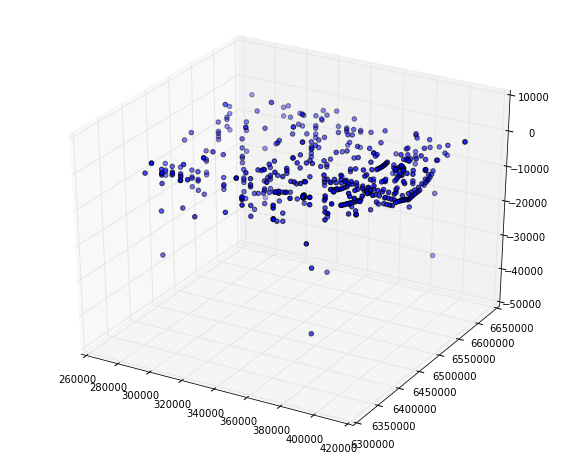
\includegraphics{3D-Structural-Data_46_0.png}

\begin{Verbatim}[commandchars=\\\{\}]
\PYG{n}{fol}\PYG{o}{.}\PYG{n}{plot\PYGZus{}plane}\PYG{p}{(}\PYG{n}{formation\PYGZus{}names} \PYG{o}{=} \PYG{l+s}{\PYGZsq{}}\PYG{l+s}{Yarragadee\PYGZus{}Fm}\PYG{l+s}{\PYGZsq{}}\PYG{p}{)}
\end{Verbatim}

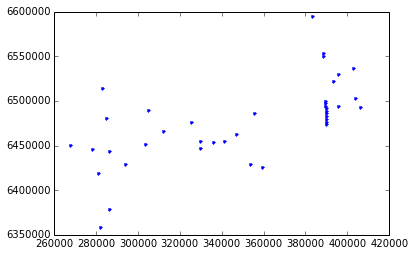
\includegraphics{3D-Structural-Data_47_0.png}


\chapter{Und das ist fuer Jan}
\label{3D-Structural-Data:und-das-ist-fuer-jan}\begin{itemize}
\item {} 
bla

\item {} 
bla2

\end{itemize}

Markdown translates

italic

This is \emph{italic} text and this is \textbf{bold}


\chapter{Creating an irregular mesh from Geomodeller for SHEMAT simulations}
\label{Geomodeller-Export::doc}\label{Geomodeller-Export:creating-an-irregular-mesh-from-geomodeller-for-shemat-simulations}
Regular meshes can be exported directly from within the Geomodeller GUI.
However, in many cases, a more flexible solution is required, for
example to:
\begin{itemize}
\item {} 
update a mesh automatically (without using the GUI), or

\item {} 
create an irregular mesh with refined regions

\end{itemize}

These steps can easily be performed with a set of Python scripts and C
programs that access Geomodellers funcionality through the API.

The main funcionality required here is combined in the Python package
\code{pygeomod}. Two main packages are required: \code{geogrid.py} is the most
recent development and contains a (relatively general) class definition
for rectangular grids in general, with the link to Geomodeller in
particular. The package ´geomodeller\_xml\_obj.py{}` contains methods to
access and modify information stored in the Geomodeller xml
Project-files. This functionality can be used, for example, to change
geological input parameters (e.g. dip of a fault) directly from the
Python script.


\bigskip\hrule{}\bigskip


A note on installation:

The most tricky part is to get the API properly installed, all libraries
linked, and compiled on a system. On esim39, the required library path
settings are defined in

\code{adjust\_to\_jni.sh}

Another important point (for now, should be fixed at some stage...) is
that the shared object \code{libgeomod.so} has to be located in the current
directory... time to write a proper make file, but to date that's the
stage the project is in.


\bigskip\hrule{}\bigskip


We will first start here with an example for the generation of an
rectilinear refined mesh for a simulation with SHEMAT.

\begin{Verbatim}[commandchars=\\\{\}]
\PYGZsh{} first step: import standard libraries and set pylab for plotting functionalities
\PYGZpc{}pylab inline
import numpy as np
import matplotlib.pyplot as plt
import sys, os
\end{Verbatim}

\begin{Verbatim}[commandchars=\\\{\}]
Welcome to pylab, a matplotlib\PYGZhy{}based Python environment [backend: module://IPython.zmq.pylab.backend\PYGZus{}inline].
For more information, type \PYGZsq{}help(pylab)\PYGZsq{}.
\end{Verbatim}

\begin{Verbatim}[commandchars=\\\{\}]
\PYG{c}{\PYGZsh{} Add path to pygeomod and import module (note: this is only required because it can\PYGZsq{}t be installed properly at the moment)}
\PYG{n}{sys}\PYG{o}{.}\PYG{n}{path}\PYG{o}{.}\PYG{n}{append}\PYG{p}{(}\PYG{l+s}{r\PYGZsq{}}\PYG{l+s}{/home/jni/git/tmp/pygeomod\PYGZus{}tmp}\PYG{l+s}{\PYGZsq{}}\PYG{p}{)}
\PYG{k+kn}{import} \PYG{n+nn}{geogrid}
\end{Verbatim}


\section{Creating a regular grid}
\label{Geomodeller-Export:creating-a-regular-grid}
The geogrid module contains a variety of methods to generate grids. In
combinbation wtih Geomodeller, the easiest thing to do is to create a
regular mesh from a Geomodeller project:

\begin{Verbatim}[commandchars=\\\{\}]
\PYG{c}{\PYGZsh{} Define path to geomodeller model file:}
\PYG{n}{geomodel} \PYG{o}{=} \PYG{l+s}{r\PYGZsq{}}\PYG{l+s}{/home/jni/git/tmp/geomuce/gemuce\PYGZus{}tmp/examples/simple\PYGZus{}three\PYGZus{}layer/simple\PYGZus{}three\PYGZus{}layer.xml}\PYG{l+s}{\PYGZsq{}}
\end{Verbatim}

\begin{Verbatim}[commandchars=\\\{\}]
\PYG{n+nb}{reload}\PYG{p}{(}\PYG{n}{geogrid}\PYG{p}{)} \PYG{c}{\PYGZsh{} only required for development stage \PYGZhy{} can be removed afterwards}
\PYG{c}{\PYGZsh{} Now: define a GeoGrid object:}
\PYG{n}{G1} \PYG{o}{=} \PYG{n}{geogrid}\PYG{o}{.}\PYG{n}{GeoGrid}\PYG{p}{(}\PYG{p}{)}
\PYG{c}{\PYGZsh{} and set the boundaries/ model extent according to the Geomodeller model:}
\PYG{n}{G1}\PYG{o}{.}\PYG{n}{get\PYGZus{}dimensions\PYGZus{}from\PYGZus{}geomodeller\PYGZus{}xml\PYGZus{}project}\PYG{p}{(}\PYG{n}{geomodel}\PYG{p}{)}
\end{Verbatim}

\begin{Verbatim}[commandchars=\\\{\}]
\PYG{c}{\PYGZsh{} and create a regular grid for a defined number of cells in each direction:}
\PYG{n}{nx} \PYG{o}{=} \PYG{l+m+mi}{25}
\PYG{n}{ny} \PYG{o}{=} \PYG{l+m+mi}{2}
\PYG{n}{nz} \PYG{o}{=} \PYG{l+m+mi}{25}
\PYG{n}{G1}\PYG{o}{.}\PYG{n}{define\PYGZus{}regular\PYGZus{}grid}\PYG{p}{(}\PYG{n}{nx}\PYG{p}{,} \PYG{n}{ny}\PYG{p}{,} \PYG{n}{nz}\PYG{p}{)}
\end{Verbatim}

\begin{Verbatim}[commandchars=\\\{\}]
\PYG{c}{\PYGZsh{} ...and, finally, update the grid properties on the base of the Geomodeller model:}
\PYG{n}{G1}\PYG{o}{.}\PYG{n}{update\PYGZus{}from\PYGZus{}geomodeller\PYGZus{}project}\PYG{p}{(}\PYG{n}{geomodel}\PYG{p}{)}
\end{Verbatim}

The grid is stored in the object variable \code{G1.grid} as a numpy array.

\begin{Verbatim}[commandchars=\\\{\}]
\PYG{n+nb}{type}\PYG{p}{(}\PYG{n}{G1}\PYG{o}{.}\PYG{n}{grid}\PYG{p}{)}
\end{Verbatim}

\begin{Verbatim}[commandchars=\\\{\}]
\PYG{n}{numpy}\PYG{o}{.}\PYG{n}{ndarray}
\end{Verbatim}

So the grid can directly be used to create slices, plots, further
caluclations, etc. However, a lot of functionality is alread implemented
in the geogrid package. For example, slice plots through the model can
simply be generated with:

\begin{Verbatim}[commandchars=\\\{\}]
\PYG{n}{G1}\PYG{o}{.}\PYG{n}{plot\PYGZus{}section}\PYG{p}{(}\PYG{l+s}{\PYGZsq{}}\PYG{l+s}{y}\PYG{l+s}{\PYGZsq{}}\PYG{p}{,} \PYG{n}{colorbar}\PYG{o}{=}\PYG{n+nb+bp}{False}\PYG{p}{,} \PYG{n}{cmap}\PYG{o}{=}\PYG{l+s}{\PYGZsq{}}\PYG{l+s}{RdBu}\PYG{l+s}{\PYGZsq{}}\PYG{p}{)} \PYG{c}{\PYGZsh{} more plotting options possible, generally following the logic of matplotlibs imshow function}
\end{Verbatim}

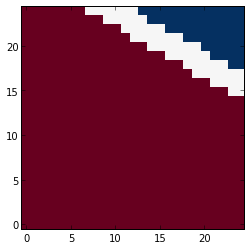
\includegraphics{Geomodeller-Export_11_0.png}

It is also possible to export the model directly to VTK - however, this
requires an installation of the pyevtk package which is not installed on
esim for now:

\begin{Verbatim}[commandchars=\\\{\}]
\PYG{n}{G1}\PYG{o}{.}\PYG{n}{export\PYGZus{}to\PYGZus{}vtk}\PYG{p}{(}\PYG{p}{)}
\end{Verbatim}

\begin{Verbatim}[commandchars=\\\{\}]
\PYGZhy{}\PYGZhy{}\PYGZhy{}\PYGZhy{}\PYGZhy{}\PYGZhy{}\PYGZhy{}\PYGZhy{}\PYGZhy{}\PYGZhy{}\PYGZhy{}\PYGZhy{}\PYGZhy{}\PYGZhy{}\PYGZhy{}\PYGZhy{}\PYGZhy{}\PYGZhy{}\PYGZhy{}\PYGZhy{}\PYGZhy{}\PYGZhy{}\PYGZhy{}\PYGZhy{}\PYGZhy{}\PYGZhy{}\PYGZhy{}\PYGZhy{}\PYGZhy{}\PYGZhy{}\PYGZhy{}\PYGZhy{}\PYGZhy{}\PYGZhy{}\PYGZhy{}\PYGZhy{}\PYGZhy{}\PYGZhy{}\PYGZhy{}\PYGZhy{}\PYGZhy{}\PYGZhy{}\PYGZhy{}\PYGZhy{}\PYGZhy{}\PYGZhy{}\PYGZhy{}\PYGZhy{}\PYGZhy{}\PYGZhy{}\PYGZhy{}\PYGZhy{}\PYGZhy{}\PYGZhy{}\PYGZhy{}\PYGZhy{}\PYGZhy{}\PYGZhy{}\PYGZhy{}\PYGZhy{}\PYGZhy{}\PYGZhy{}\PYGZhy{}\PYGZhy{}\PYGZhy{}\PYGZhy{}\PYGZhy{}\PYGZhy{}\PYGZhy{}\PYGZhy{}\PYGZhy{}\PYGZhy{}\PYGZhy{}\PYGZhy{}\PYGZhy{}
ImportError                               Traceback (most recent call last)

\PYGZlt{}ipython\PYGZhy{}input\PYGZhy{}71\PYGZhy{}972ad06a1420\PYGZgt{} in \PYGZlt{}module\PYGZgt{}()
\PYGZhy{}\PYGZhy{}\PYGZhy{}\PYGZhy{}\PYGZgt{} 1 G1.export\PYGZus{}to\PYGZus{}vtk()


/home/jni/git/tmp/pygeomod\PYGZus{}tmp/geogrid.py in export\PYGZus{}to\PYGZus{}vtk(self, vtk\PYGZus{}filename, real\PYGZus{}coords, **kwds)
    327         grid = kwds.get(\PYGZdq{}grid\PYGZdq{}, self.grid)
    328         var\PYGZus{}name = kwds.get(\PYGZdq{}var\PYGZus{}name\PYGZdq{}, \PYGZdq{}Geology\PYGZdq{})
\PYGZhy{}\PYGZhy{}\PYGZgt{} 329         from evtk.hl import gridToVTK
    330         \PYGZsh{} define coordinates
    331         x = np.zeros(self.nx + 1)


ImportError: No module named evtk.hl
\end{Verbatim}


\section{Rectilinear grids}
\label{Geomodeller-Export:rectilinear-grids}
Creating a rectilinear grid requires only that the cell spacings are
explicitly defined. Everything else is exactly the same as before. Note
that it is (at the moment) your responsibility to assing proper spacings
- if you go beyond the bounds of the Geomodel, the function will not
crash, but return the standard Geomodeller ``out'' value (usually the
number of stratigraphic units + 1).

One way to create meshes in the correct range is, of course, to use the
extent of the Geomodel, determined with the function:

\begin{Verbatim}[commandchars=\\\{\}]
\PYG{n+nb}{reload}\PYG{p}{(}\PYG{n}{geogrid}\PYG{p}{)} \PYG{c}{\PYGZsh{} only required for development stage \PYGZhy{} can be removed afterwards}
\PYG{c}{\PYGZsh{} Now: define a GeoGrid object:}
\PYG{n}{G1} \PYG{o}{=} \PYG{n}{geogrid}\PYG{o}{.}\PYG{n}{GeoGrid}\PYG{p}{(}\PYG{p}{)}
\PYG{c}{\PYGZsh{} and set the boundaries/ model extent according to the Geomodeller model:}
\PYG{n}{G1}\PYG{o}{.}\PYG{n}{get\PYGZus{}dimensions\PYGZus{}from\PYGZus{}geomodeller\PYGZus{}xml\PYGZus{}project}\PYG{p}{(}\PYG{n}{geomodel}\PYG{p}{)}
\end{Verbatim}

\begin{Verbatim}[commandchars=\\\{\}]
\PYG{c}{\PYGZsh{} The extent of the Geomodeller model can be obtained with:}
\PYG{n}{G1}\PYG{o}{.}\PYG{n}{xmin}\PYG{p}{,} \PYG{n}{G1}\PYG{o}{.}\PYG{n}{xmax}
\end{Verbatim}

\begin{Verbatim}[commandchars=\\\{\}]
\PYG{p}{(}\PYG{l+m+mi}{0}\PYG{p}{,} \PYG{l+m+mi}{1000}\PYG{p}{)}
\end{Verbatim}

\begin{Verbatim}[commandchars=\\\{\}]
\PYG{c}{\PYGZsh{} and the extent with:}
\PYG{n}{G1}\PYG{o}{.}\PYG{n}{extent\PYGZus{}x}
\end{Verbatim}

\begin{Verbatim}[commandchars=\\\{\}]
\PYG{l+m+mi}{1000}
\end{Verbatim}

Let's be a bit fancy and create the horizontal (x,y) grid with a core
region of high refinement and increasing mesh sizes towards the
boundary. First, we define the geometry:

\begin{Verbatim}[commandchars=\\\{\}]
\PYG{n}{core\PYGZus{}region} \PYG{o}{=} \PYG{l+m+mi}{100} \PYG{c}{\PYGZsh{} m}
\PYG{c}{\PYGZsh{} define cell width in core region:}
\PYG{n}{cell\PYGZus{}width\PYGZus{}core} \PYG{o}{=} \PYG{l+m+mi}{25} \PYG{c}{\PYGZsh{} m}
\PYG{n}{del\PYGZus{}core} \PYG{o}{=} \PYG{n}{np}\PYG{o}{.}\PYG{n}{ones}\PYG{p}{(}\PYG{n+nb}{int}\PYG{p}{(}\PYG{n}{core\PYGZus{}region} \PYG{o}{/} \PYG{n}{cell\PYGZus{}width\PYGZus{}core}\PYG{p}{)}\PYG{p}{)} \PYG{o}{*} \PYG{n}{cell\PYGZus{}width\PYGZus{}core}
\PYG{c}{\PYGZsh{} and the number of cells in the boundary regions (the innermost cell has the size of the core cells):}
\PYG{n}{n\PYGZus{}boundary} \PYG{o}{=} \PYG{l+m+mi}{10}
\PYG{c}{\PYGZsh{} now determine the boundary width on both sides of the core region:}
\PYG{n}{width\PYGZus{}boundary\PYGZus{}x} \PYG{o}{=} \PYG{p}{(}\PYG{n}{G1}\PYG{o}{.}\PYG{n}{extent\PYGZus{}x} \PYG{o}{\PYGZhy{}} \PYG{n}{core\PYGZus{}region}\PYG{p}{)} \PYG{o}{/} \PYG{l+m+mf}{2.}
\PYG{n}{width\PYGZus{}boundary\PYGZus{}y} \PYG{o}{=} \PYG{p}{(}\PYG{n}{G1}\PYG{o}{.}\PYG{n}{extent\PYGZus{}y} \PYG{o}{\PYGZhy{}} \PYG{n}{core\PYGZus{}region}\PYG{p}{)} \PYG{o}{/} \PYG{l+m+mf}{2.}
\end{Verbatim}

A little helper function in the \code{geogrid} package can be used to
determine an optimal cell increase factor for the boundary cells for a
given width an a number of cells, and a fixed inner cell width which we
take as the width of the core cells for a neat transition:

\begin{Verbatim}[commandchars=\\\{\}]
\PYG{n}{dx\PYGZus{}boundary} \PYG{o}{=} \PYG{n}{geogrid}\PYG{o}{.}\PYG{n}{optimial\PYGZus{}cell\PYGZus{}increase}\PYG{p}{(}\PYG{n}{cell\PYGZus{}width\PYGZus{}core}\PYG{p}{,} \PYG{n}{n\PYGZus{}boundary}\PYG{p}{,} \PYG{n}{width\PYGZus{}boundary\PYGZus{}x}\PYG{p}{)}
\PYG{n}{dy\PYGZus{}boundary} \PYG{o}{=} \PYG{n}{geogrid}\PYG{o}{.}\PYG{n}{optimial\PYGZus{}cell\PYGZus{}increase}\PYG{p}{(}\PYG{n}{cell\PYGZus{}width\PYGZus{}core}\PYG{p}{,} \PYG{n}{n\PYGZus{}boundary}\PYG{p}{,} \PYG{n}{width\PYGZus{}boundary\PYGZus{}y}\PYG{p}{)}
\end{Verbatim}

We now simply combine the boundary and core cells for the complete
discretisation array:

\begin{Verbatim}[commandchars=\\\{\}]
\PYG{n}{delx} \PYG{o}{=} \PYG{n}{np}\PYG{o}{.}\PYG{n}{concatenate}\PYG{p}{(}\PYG{p}{(}\PYG{n}{dx\PYGZus{}boundary}\PYG{p}{[}\PYG{p}{:}\PYG{p}{:}\PYG{o}{\PYGZhy{}}\PYG{l+m+mi}{1}\PYG{p}{]}\PYG{p}{,} \PYG{n}{del\PYGZus{}core}\PYG{p}{,} \PYG{n}{dx\PYGZus{}boundary}\PYG{p}{)}\PYG{p}{)} \PYG{c}{\PYGZsh{} first array reversed from large to small cells}
\PYG{n}{dely} \PYG{o}{=} \PYG{n}{np}\PYG{o}{.}\PYG{n}{concatenate}\PYG{p}{(}\PYG{p}{(}\PYG{n}{dy\PYGZus{}boundary}\PYG{p}{[}\PYG{p}{:}\PYG{p}{:}\PYG{o}{\PYGZhy{}}\PYG{l+m+mi}{1}\PYG{p}{]}\PYG{p}{,} \PYG{n}{del\PYGZus{}core}\PYG{p}{,} \PYG{n}{dy\PYGZus{}boundary}\PYG{p}{)}\PYG{p}{)}
\end{Verbatim}

A plot of the grid:

\begin{Verbatim}[commandchars=\\\{\}]
\PYG{n}{fig} \PYG{o}{=} \PYG{n}{plt}\PYG{o}{.}\PYG{n}{figure}\PYG{p}{(}\PYG{n}{figsize} \PYG{o}{=} \PYG{p}{(}\PYG{l+m+mi}{8}\PYG{p}{,}\PYG{l+m+mi}{8}\PYG{p}{)}\PYG{p}{)}
\PYG{n}{ax} \PYG{o}{=} \PYG{n}{fig}\PYG{o}{.}\PYG{n}{add\PYGZus{}subplot}\PYG{p}{(}\PYG{l+m+mi}{111}\PYG{p}{)}
\PYG{k}{for} \PYG{n}{dx} \PYG{o+ow}{in} \PYG{n}{np}\PYG{o}{.}\PYG{n}{cumsum}\PYG{p}{(}\PYG{n}{delx}\PYG{p}{)}\PYG{p}{:}
    \PYG{n}{ax}\PYG{o}{.}\PYG{n}{axvline}\PYG{p}{(}\PYG{n}{dx}\PYG{p}{,} \PYG{n}{color} \PYG{o}{=} \PYG{l+s}{\PYGZsq{}}\PYG{l+s}{k}\PYG{l+s}{\PYGZsq{}}\PYG{p}{)}
\PYG{k}{for} \PYG{n}{dy} \PYG{o+ow}{in} \PYG{n}{np}\PYG{o}{.}\PYG{n}{cumsum}\PYG{p}{(}\PYG{n}{dely}\PYG{p}{)}\PYG{p}{:}
    \PYG{n}{ax}\PYG{o}{.}\PYG{n}{axhline}\PYG{p}{(}\PYG{n}{dy}\PYG{p}{,} \PYG{n}{color} \PYG{o}{=} \PYG{l+s}{\PYGZsq{}}\PYG{l+s}{k}\PYG{l+s}{\PYGZsq{}}\PYG{p}{)}

\PYG{n}{ax}\PYG{o}{.}\PYG{n}{set\PYGZus{}xlim}\PYG{p}{(}\PYG{p}{(}\PYG{l+m+mi}{0}\PYG{p}{,}\PYG{n+nb}{sum}\PYG{p}{(}\PYG{n}{delx}\PYG{p}{)}\PYG{p}{)}\PYG{p}{)}
\PYG{n}{ax}\PYG{o}{.}\PYG{n}{set\PYGZus{}ylim}\PYG{p}{(}\PYG{p}{(}\PYG{l+m+mi}{0}\PYG{p}{,}\PYG{n+nb}{sum}\PYG{p}{(}\PYG{n}{dely}\PYG{p}{)}\PYG{p}{)}\PYG{p}{)}
\end{Verbatim}

\begin{Verbatim}[commandchars=\\\{\}]
\PYG{p}{(}\PYG{l+m+mi}{0}\PYG{p}{,} \PYG{l+m+mf}{999.99999999999864}\PYG{p}{)}
\end{Verbatim}

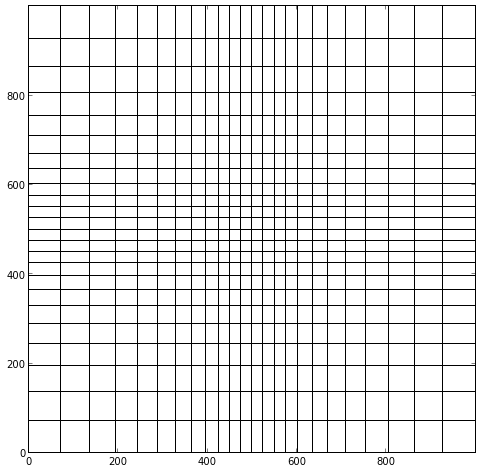
\includegraphics{Geomodeller-Export_25_1.png}

In z-direction we will create a regular mesh:

\begin{Verbatim}[commandchars=\\\{\}]
\PYG{n}{nz} \PYG{o}{=} \PYG{l+m+mi}{20}
\PYG{n}{delz} \PYG{o}{=} \PYG{n}{np}\PYG{o}{.}\PYG{n}{ones}\PYG{p}{(}\PYG{n}{nz}\PYG{p}{)} \PYG{o}{*} \PYG{n}{G1}\PYG{o}{.}\PYG{n}{extent\PYGZus{}z} \PYG{o}{/} \PYG{n}{nz}
\end{Verbatim}

Ok, back to the geogrid package: we now assign the cell discretisation
arrays to the geogrid object and populate the grid with geology ids
determined from the Geomodeller model:

\begin{Verbatim}[commandchars=\\\{\}]
\PYG{n}{G1}\PYG{o}{.}\PYG{n}{define\PYGZus{}irregular\PYGZus{}grid}\PYG{p}{(}\PYG{n}{delx}\PYG{p}{,} \PYG{n}{dely}\PYG{p}{,} \PYG{n}{delz}\PYG{p}{)}
\PYG{n}{G1}\PYG{o}{.}\PYG{n}{update\PYGZus{}from\PYGZus{}geomodeller\PYGZus{}project}\PYG{p}{(}\PYG{n}{geomodel}\PYG{p}{)}
\end{Verbatim}

\begin{Verbatim}[commandchars=\\\{\}]
\PYG{n}{G1}\PYG{o}{.}\PYG{n}{grid}
\end{Verbatim}

\begin{Verbatim}[commandchars=\\\{\}]
\PYG{n}{array}\PYG{p}{(}\PYG{p}{[}\PYG{p}{[}\PYG{p}{[} \PYG{l+m+mf}{1.}\PYG{p}{,}  \PYG{l+m+mf}{1.}\PYG{p}{,}  \PYG{l+m+mf}{1.}\PYG{p}{,} \PYG{o}{.}\PYG{o}{.}\PYG{o}{.}\PYG{p}{,}  \PYG{l+m+mf}{1.}\PYG{p}{,}  \PYG{l+m+mf}{1.}\PYG{p}{,}  \PYG{l+m+mf}{1.}\PYG{p}{]}\PYG{p}{,}
        \PYG{p}{[} \PYG{l+m+mf}{1.}\PYG{p}{,}  \PYG{l+m+mf}{1.}\PYG{p}{,}  \PYG{l+m+mf}{1.}\PYG{p}{,} \PYG{o}{.}\PYG{o}{.}\PYG{o}{.}\PYG{p}{,}  \PYG{l+m+mf}{1.}\PYG{p}{,}  \PYG{l+m+mf}{1.}\PYG{p}{,}  \PYG{l+m+mf}{1.}\PYG{p}{]}\PYG{p}{,}
        \PYG{p}{[} \PYG{l+m+mf}{1.}\PYG{p}{,}  \PYG{l+m+mf}{1.}\PYG{p}{,}  \PYG{l+m+mf}{1.}\PYG{p}{,} \PYG{o}{.}\PYG{o}{.}\PYG{o}{.}\PYG{p}{,}  \PYG{l+m+mf}{1.}\PYG{p}{,}  \PYG{l+m+mf}{1.}\PYG{p}{,}  \PYG{l+m+mf}{1.}\PYG{p}{]}\PYG{p}{,}
        \PYG{o}{.}\PYG{o}{.}\PYG{o}{.}\PYG{p}{,}
        \PYG{p}{[} \PYG{l+m+mf}{1.}\PYG{p}{,}  \PYG{l+m+mf}{1.}\PYG{p}{,}  \PYG{l+m+mf}{1.}\PYG{p}{,} \PYG{o}{.}\PYG{o}{.}\PYG{o}{.}\PYG{p}{,}  \PYG{l+m+mf}{1.}\PYG{p}{,}  \PYG{l+m+mf}{1.}\PYG{p}{,}  \PYG{l+m+mf}{1.}\PYG{p}{]}\PYG{p}{,}
        \PYG{p}{[} \PYG{l+m+mf}{1.}\PYG{p}{,}  \PYG{l+m+mf}{1.}\PYG{p}{,}  \PYG{l+m+mf}{1.}\PYG{p}{,} \PYG{o}{.}\PYG{o}{.}\PYG{o}{.}\PYG{p}{,}  \PYG{l+m+mf}{1.}\PYG{p}{,}  \PYG{l+m+mf}{1.}\PYG{p}{,}  \PYG{l+m+mf}{1.}\PYG{p}{]}\PYG{p}{,}
        \PYG{p}{[} \PYG{l+m+mf}{1.}\PYG{p}{,}  \PYG{l+m+mf}{1.}\PYG{p}{,}  \PYG{l+m+mf}{1.}\PYG{p}{,} \PYG{o}{.}\PYG{o}{.}\PYG{o}{.}\PYG{p}{,}  \PYG{l+m+mf}{1.}\PYG{p}{,}  \PYG{l+m+mf}{1.}\PYG{p}{,}  \PYG{l+m+mf}{1.}\PYG{p}{]}\PYG{p}{]}\PYG{p}{,}

       \PYG{p}{[}\PYG{p}{[} \PYG{l+m+mf}{1.}\PYG{p}{,}  \PYG{l+m+mf}{1.}\PYG{p}{,}  \PYG{l+m+mf}{1.}\PYG{p}{,} \PYG{o}{.}\PYG{o}{.}\PYG{o}{.}\PYG{p}{,}  \PYG{l+m+mf}{1.}\PYG{p}{,}  \PYG{l+m+mf}{1.}\PYG{p}{,}  \PYG{l+m+mf}{1.}\PYG{p}{]}\PYG{p}{,}
        \PYG{p}{[} \PYG{l+m+mf}{1.}\PYG{p}{,}  \PYG{l+m+mf}{1.}\PYG{p}{,}  \PYG{l+m+mf}{1.}\PYG{p}{,} \PYG{o}{.}\PYG{o}{.}\PYG{o}{.}\PYG{p}{,}  \PYG{l+m+mf}{1.}\PYG{p}{,}  \PYG{l+m+mf}{1.}\PYG{p}{,}  \PYG{l+m+mf}{1.}\PYG{p}{]}\PYG{p}{,}
        \PYG{p}{[} \PYG{l+m+mf}{1.}\PYG{p}{,}  \PYG{l+m+mf}{1.}\PYG{p}{,}  \PYG{l+m+mf}{1.}\PYG{p}{,} \PYG{o}{.}\PYG{o}{.}\PYG{o}{.}\PYG{p}{,}  \PYG{l+m+mf}{1.}\PYG{p}{,}  \PYG{l+m+mf}{1.}\PYG{p}{,}  \PYG{l+m+mf}{1.}\PYG{p}{]}\PYG{p}{,}
        \PYG{o}{.}\PYG{o}{.}\PYG{o}{.}\PYG{p}{,}
        \PYG{p}{[} \PYG{l+m+mf}{1.}\PYG{p}{,}  \PYG{l+m+mf}{1.}\PYG{p}{,}  \PYG{l+m+mf}{1.}\PYG{p}{,} \PYG{o}{.}\PYG{o}{.}\PYG{o}{.}\PYG{p}{,}  \PYG{l+m+mf}{1.}\PYG{p}{,}  \PYG{l+m+mf}{1.}\PYG{p}{,}  \PYG{l+m+mf}{1.}\PYG{p}{]}\PYG{p}{,}
        \PYG{p}{[} \PYG{l+m+mf}{1.}\PYG{p}{,}  \PYG{l+m+mf}{1.}\PYG{p}{,}  \PYG{l+m+mf}{1.}\PYG{p}{,} \PYG{o}{.}\PYG{o}{.}\PYG{o}{.}\PYG{p}{,}  \PYG{l+m+mf}{1.}\PYG{p}{,}  \PYG{l+m+mf}{1.}\PYG{p}{,}  \PYG{l+m+mf}{1.}\PYG{p}{]}\PYG{p}{,}
        \PYG{p}{[} \PYG{l+m+mf}{1.}\PYG{p}{,}  \PYG{l+m+mf}{1.}\PYG{p}{,}  \PYG{l+m+mf}{1.}\PYG{p}{,} \PYG{o}{.}\PYG{o}{.}\PYG{o}{.}\PYG{p}{,}  \PYG{l+m+mf}{1.}\PYG{p}{,}  \PYG{l+m+mf}{1.}\PYG{p}{,}  \PYG{l+m+mf}{1.}\PYG{p}{]}\PYG{p}{]}\PYG{p}{,}

       \PYG{p}{[}\PYG{p}{[} \PYG{l+m+mf}{1.}\PYG{p}{,}  \PYG{l+m+mf}{1.}\PYG{p}{,}  \PYG{l+m+mf}{1.}\PYG{p}{,} \PYG{o}{.}\PYG{o}{.}\PYG{o}{.}\PYG{p}{,}  \PYG{l+m+mf}{1.}\PYG{p}{,}  \PYG{l+m+mf}{1.}\PYG{p}{,}  \PYG{l+m+mf}{1.}\PYG{p}{]}\PYG{p}{,}
        \PYG{p}{[} \PYG{l+m+mf}{1.}\PYG{p}{,}  \PYG{l+m+mf}{1.}\PYG{p}{,}  \PYG{l+m+mf}{1.}\PYG{p}{,} \PYG{o}{.}\PYG{o}{.}\PYG{o}{.}\PYG{p}{,}  \PYG{l+m+mf}{1.}\PYG{p}{,}  \PYG{l+m+mf}{1.}\PYG{p}{,}  \PYG{l+m+mf}{1.}\PYG{p}{]}\PYG{p}{,}
        \PYG{p}{[} \PYG{l+m+mf}{1.}\PYG{p}{,}  \PYG{l+m+mf}{1.}\PYG{p}{,}  \PYG{l+m+mf}{1.}\PYG{p}{,} \PYG{o}{.}\PYG{o}{.}\PYG{o}{.}\PYG{p}{,}  \PYG{l+m+mf}{1.}\PYG{p}{,}  \PYG{l+m+mf}{1.}\PYG{p}{,}  \PYG{l+m+mf}{1.}\PYG{p}{]}\PYG{p}{,}
        \PYG{o}{.}\PYG{o}{.}\PYG{o}{.}\PYG{p}{,}
        \PYG{p}{[} \PYG{l+m+mf}{1.}\PYG{p}{,}  \PYG{l+m+mf}{1.}\PYG{p}{,}  \PYG{l+m+mf}{1.}\PYG{p}{,} \PYG{o}{.}\PYG{o}{.}\PYG{o}{.}\PYG{p}{,}  \PYG{l+m+mf}{1.}\PYG{p}{,}  \PYG{l+m+mf}{1.}\PYG{p}{,}  \PYG{l+m+mf}{1.}\PYG{p}{]}\PYG{p}{,}
        \PYG{p}{[} \PYG{l+m+mf}{1.}\PYG{p}{,}  \PYG{l+m+mf}{1.}\PYG{p}{,}  \PYG{l+m+mf}{1.}\PYG{p}{,} \PYG{o}{.}\PYG{o}{.}\PYG{o}{.}\PYG{p}{,}  \PYG{l+m+mf}{1.}\PYG{p}{,}  \PYG{l+m+mf}{1.}\PYG{p}{,}  \PYG{l+m+mf}{1.}\PYG{p}{]}\PYG{p}{,}
        \PYG{p}{[} \PYG{l+m+mf}{1.}\PYG{p}{,}  \PYG{l+m+mf}{1.}\PYG{p}{,}  \PYG{l+m+mf}{1.}\PYG{p}{,} \PYG{o}{.}\PYG{o}{.}\PYG{o}{.}\PYG{p}{,}  \PYG{l+m+mf}{1.}\PYG{p}{,}  \PYG{l+m+mf}{1.}\PYG{p}{,}  \PYG{l+m+mf}{1.}\PYG{p}{]}\PYG{p}{]}\PYG{p}{,}

       \PYG{o}{.}\PYG{o}{.}\PYG{o}{.}\PYG{p}{,}
       \PYG{p}{[}\PYG{p}{[} \PYG{l+m+mf}{1.}\PYG{p}{,}  \PYG{l+m+mf}{1.}\PYG{p}{,}  \PYG{l+m+mf}{1.}\PYG{p}{,} \PYG{o}{.}\PYG{o}{.}\PYG{o}{.}\PYG{p}{,}  \PYG{l+m+mf}{3.}\PYG{p}{,}  \PYG{l+m+mf}{3.}\PYG{p}{,}  \PYG{l+m+mf}{3.}\PYG{p}{]}\PYG{p}{,}
        \PYG{p}{[} \PYG{l+m+mf}{1.}\PYG{p}{,}  \PYG{l+m+mf}{1.}\PYG{p}{,}  \PYG{l+m+mf}{1.}\PYG{p}{,} \PYG{o}{.}\PYG{o}{.}\PYG{o}{.}\PYG{p}{,}  \PYG{l+m+mf}{3.}\PYG{p}{,}  \PYG{l+m+mf}{3.}\PYG{p}{,}  \PYG{l+m+mf}{3.}\PYG{p}{]}\PYG{p}{,}
        \PYG{p}{[} \PYG{l+m+mf}{1.}\PYG{p}{,}  \PYG{l+m+mf}{1.}\PYG{p}{,}  \PYG{l+m+mf}{1.}\PYG{p}{,} \PYG{o}{.}\PYG{o}{.}\PYG{o}{.}\PYG{p}{,}  \PYG{l+m+mf}{3.}\PYG{p}{,}  \PYG{l+m+mf}{3.}\PYG{p}{,}  \PYG{l+m+mf}{3.}\PYG{p}{]}\PYG{p}{,}
        \PYG{o}{.}\PYG{o}{.}\PYG{o}{.}\PYG{p}{,}
        \PYG{p}{[} \PYG{l+m+mf}{1.}\PYG{p}{,}  \PYG{l+m+mf}{1.}\PYG{p}{,}  \PYG{l+m+mf}{1.}\PYG{p}{,} \PYG{o}{.}\PYG{o}{.}\PYG{o}{.}\PYG{p}{,}  \PYG{l+m+mf}{3.}\PYG{p}{,}  \PYG{l+m+mf}{3.}\PYG{p}{,}  \PYG{l+m+mf}{3.}\PYG{p}{]}\PYG{p}{,}
        \PYG{p}{[} \PYG{l+m+mf}{1.}\PYG{p}{,}  \PYG{l+m+mf}{1.}\PYG{p}{,}  \PYG{l+m+mf}{1.}\PYG{p}{,} \PYG{o}{.}\PYG{o}{.}\PYG{o}{.}\PYG{p}{,}  \PYG{l+m+mf}{3.}\PYG{p}{,}  \PYG{l+m+mf}{3.}\PYG{p}{,}  \PYG{l+m+mf}{3.}\PYG{p}{]}\PYG{p}{,}
        \PYG{p}{[} \PYG{l+m+mf}{1.}\PYG{p}{,}  \PYG{l+m+mf}{1.}\PYG{p}{,}  \PYG{l+m+mf}{1.}\PYG{p}{,} \PYG{o}{.}\PYG{o}{.}\PYG{o}{.}\PYG{p}{,}  \PYG{l+m+mf}{3.}\PYG{p}{,}  \PYG{l+m+mf}{3.}\PYG{p}{,}  \PYG{l+m+mf}{3.}\PYG{p}{]}\PYG{p}{]}\PYG{p}{,}

       \PYG{p}{[}\PYG{p}{[} \PYG{l+m+mf}{1.}\PYG{p}{,}  \PYG{l+m+mf}{1.}\PYG{p}{,}  \PYG{l+m+mf}{1.}\PYG{p}{,} \PYG{o}{.}\PYG{o}{.}\PYG{o}{.}\PYG{p}{,}  \PYG{l+m+mf}{3.}\PYG{p}{,}  \PYG{l+m+mf}{3.}\PYG{p}{,}  \PYG{l+m+mf}{3.}\PYG{p}{]}\PYG{p}{,}
        \PYG{p}{[} \PYG{l+m+mf}{1.}\PYG{p}{,}  \PYG{l+m+mf}{1.}\PYG{p}{,}  \PYG{l+m+mf}{1.}\PYG{p}{,} \PYG{o}{.}\PYG{o}{.}\PYG{o}{.}\PYG{p}{,}  \PYG{l+m+mf}{3.}\PYG{p}{,}  \PYG{l+m+mf}{3.}\PYG{p}{,}  \PYG{l+m+mf}{3.}\PYG{p}{]}\PYG{p}{,}
        \PYG{p}{[} \PYG{l+m+mf}{1.}\PYG{p}{,}  \PYG{l+m+mf}{1.}\PYG{p}{,}  \PYG{l+m+mf}{1.}\PYG{p}{,} \PYG{o}{.}\PYG{o}{.}\PYG{o}{.}\PYG{p}{,}  \PYG{l+m+mf}{3.}\PYG{p}{,}  \PYG{l+m+mf}{3.}\PYG{p}{,}  \PYG{l+m+mf}{3.}\PYG{p}{]}\PYG{p}{,}
        \PYG{o}{.}\PYG{o}{.}\PYG{o}{.}\PYG{p}{,}
        \PYG{p}{[} \PYG{l+m+mf}{1.}\PYG{p}{,}  \PYG{l+m+mf}{1.}\PYG{p}{,}  \PYG{l+m+mf}{1.}\PYG{p}{,} \PYG{o}{.}\PYG{o}{.}\PYG{o}{.}\PYG{p}{,}  \PYG{l+m+mf}{3.}\PYG{p}{,}  \PYG{l+m+mf}{3.}\PYG{p}{,}  \PYG{l+m+mf}{3.}\PYG{p}{]}\PYG{p}{,}
        \PYG{p}{[} \PYG{l+m+mf}{1.}\PYG{p}{,}  \PYG{l+m+mf}{1.}\PYG{p}{,}  \PYG{l+m+mf}{1.}\PYG{p}{,} \PYG{o}{.}\PYG{o}{.}\PYG{o}{.}\PYG{p}{,}  \PYG{l+m+mf}{3.}\PYG{p}{,}  \PYG{l+m+mf}{3.}\PYG{p}{,}  \PYG{l+m+mf}{3.}\PYG{p}{]}\PYG{p}{,}
        \PYG{p}{[} \PYG{l+m+mf}{1.}\PYG{p}{,}  \PYG{l+m+mf}{1.}\PYG{p}{,}  \PYG{l+m+mf}{1.}\PYG{p}{,} \PYG{o}{.}\PYG{o}{.}\PYG{o}{.}\PYG{p}{,}  \PYG{l+m+mf}{3.}\PYG{p}{,}  \PYG{l+m+mf}{3.}\PYG{p}{,}  \PYG{l+m+mf}{3.}\PYG{p}{]}\PYG{p}{]}\PYG{p}{,}

       \PYG{p}{[}\PYG{p}{[} \PYG{l+m+mf}{1.}\PYG{p}{,}  \PYG{l+m+mf}{1.}\PYG{p}{,}  \PYG{l+m+mf}{1.}\PYG{p}{,} \PYG{o}{.}\PYG{o}{.}\PYG{o}{.}\PYG{p}{,}  \PYG{l+m+mf}{3.}\PYG{p}{,}  \PYG{l+m+mf}{3.}\PYG{p}{,}  \PYG{l+m+mf}{3.}\PYG{p}{]}\PYG{p}{,}
        \PYG{p}{[} \PYG{l+m+mf}{1.}\PYG{p}{,}  \PYG{l+m+mf}{1.}\PYG{p}{,}  \PYG{l+m+mf}{1.}\PYG{p}{,} \PYG{o}{.}\PYG{o}{.}\PYG{o}{.}\PYG{p}{,}  \PYG{l+m+mf}{3.}\PYG{p}{,}  \PYG{l+m+mf}{3.}\PYG{p}{,}  \PYG{l+m+mf}{3.}\PYG{p}{]}\PYG{p}{,}
        \PYG{p}{[} \PYG{l+m+mf}{1.}\PYG{p}{,}  \PYG{l+m+mf}{1.}\PYG{p}{,}  \PYG{l+m+mf}{1.}\PYG{p}{,} \PYG{o}{.}\PYG{o}{.}\PYG{o}{.}\PYG{p}{,}  \PYG{l+m+mf}{3.}\PYG{p}{,}  \PYG{l+m+mf}{3.}\PYG{p}{,}  \PYG{l+m+mf}{3.}\PYG{p}{]}\PYG{p}{,}
        \PYG{o}{.}\PYG{o}{.}\PYG{o}{.}\PYG{p}{,}
        \PYG{p}{[} \PYG{l+m+mf}{1.}\PYG{p}{,}  \PYG{l+m+mf}{1.}\PYG{p}{,}  \PYG{l+m+mf}{1.}\PYG{p}{,} \PYG{o}{.}\PYG{o}{.}\PYG{o}{.}\PYG{p}{,}  \PYG{l+m+mf}{3.}\PYG{p}{,}  \PYG{l+m+mf}{3.}\PYG{p}{,}  \PYG{l+m+mf}{3.}\PYG{p}{]}\PYG{p}{,}
        \PYG{p}{[} \PYG{l+m+mf}{1.}\PYG{p}{,}  \PYG{l+m+mf}{1.}\PYG{p}{,}  \PYG{l+m+mf}{1.}\PYG{p}{,} \PYG{o}{.}\PYG{o}{.}\PYG{o}{.}\PYG{p}{,}  \PYG{l+m+mf}{3.}\PYG{p}{,}  \PYG{l+m+mf}{3.}\PYG{p}{,}  \PYG{l+m+mf}{3.}\PYG{p}{]}\PYG{p}{,}
        \PYG{p}{[} \PYG{l+m+mf}{1.}\PYG{p}{,}  \PYG{l+m+mf}{1.}\PYG{p}{,}  \PYG{l+m+mf}{1.}\PYG{p}{,} \PYG{o}{.}\PYG{o}{.}\PYG{o}{.}\PYG{p}{,}  \PYG{l+m+mf}{3.}\PYG{p}{,}  \PYG{l+m+mf}{3.}\PYG{p}{,}  \PYG{l+m+mf}{3.}\PYG{p}{]}\PYG{p}{]}\PYG{p}{]}\PYG{p}{)}
\end{Verbatim}

The simple plotting functions don't work for irregular/ rectilinear
grids at to date (as imshow can only plot regular grids). Export to VTK
would work, in principle.

What we can do, however, is create a SHEMAT nml file (for the old SHEMAT
version) directly from the grid:

\begin{Verbatim}[commandchars=\\\{\}]
\PYG{n}{sys}\PYG{o}{.}\PYG{n}{path}\PYG{o}{.}\PYG{n}{append}\PYG{p}{(}\PYG{l+s}{r\PYGZsq{}}\PYG{l+s}{/home/jni/git/tmp/PySHEMAT/PySHEMAT\PYGZhy{}master}\PYG{l+s}{\PYGZsq{}}\PYG{p}{)}
\PYG{k+kn}{import} \PYG{n+nn}{PySHEMAT}
\end{Verbatim}

\begin{Verbatim}[commandchars=\\\{\}]
\PYG{n}{S1} \PYG{o}{=} \PYG{n}{PySHEMAT}\PYG{o}{.}\PYG{n}{Shemat\PYGZus{}file}\PYG{p}{(}\PYG{n}{from\PYGZus{}geogrid} \PYG{o}{=} \PYG{n}{G1}\PYG{p}{,} \PYG{n}{nml\PYGZus{}filename} \PYG{o}{=} \PYG{l+s}{\PYGZsq{}}\PYG{l+s}{updated\PYGZus{}model.nml}\PYG{l+s}{\PYGZsq{}}\PYG{p}{)}
\end{Verbatim}

\begin{Verbatim}[commandchars=\\\{\}]
create empty file
\end{Verbatim}


\chapter{pygeomod}
\label{modules:pygeomod}\label{modules::doc}

\section{pygeomod package}
\label{pygeomod::doc}\label{pygeomod:pygeomod-package}

\subsection{Submodules}
\label{pygeomod:submodules}

\subsection{pygeomod.geogrid module}
\label{pygeomod:module-pygeomod.geogrid}\label{pygeomod:pygeomod-geogrid-module}\index{pygeomod.geogrid (module)}
Module with classes and methods to analyse and process exported geomodel grids

Created on 21/03/2014

@author: Florian Wellmann (some parts originally developed by Erik Schaeffer)
\index{GeoGrid (class in pygeomod.geogrid)}

\begin{fulllineitems}
\phantomsection\label{pygeomod:pygeomod.geogrid.GeoGrid}\pysiglinewithargsret{\strong{class }\code{pygeomod.geogrid.}\bfcode{GeoGrid}}{\emph{**kwds}}{}
Object definition for exported geomodel grids
\index{adjust\_gridshape() (pygeomod.geogrid.GeoGrid method)}

\begin{fulllineitems}
\phantomsection\label{pygeomod:pygeomod.geogrid.GeoGrid.adjust_gridshape}\pysiglinewithargsret{\bfcode{adjust\_gridshape}}{}{}
Reshape numpy array to reflect model dimensions

\end{fulllineitems}

\index{define\_irregular\_grid() (pygeomod.geogrid.GeoGrid method)}

\begin{fulllineitems}
\phantomsection\label{pygeomod:pygeomod.geogrid.GeoGrid.define_irregular_grid}\pysiglinewithargsret{\bfcode{define\_irregular\_grid}}{\emph{delx}, \emph{dely}, \emph{delz}}{}
Set irregular grid according to delimter arrays in each direction

\end{fulllineitems}

\index{define\_regular\_grid() (pygeomod.geogrid.GeoGrid method)}

\begin{fulllineitems}
\phantomsection\label{pygeomod:pygeomod.geogrid.GeoGrid.define_regular_grid}\pysiglinewithargsret{\bfcode{define\_regular\_grid}}{\emph{nx}, \emph{ny}, \emph{nz}}{}
Define a regular grid from defined project boundaries and given discretisations

\end{fulllineitems}

\index{determine\_cell\_centers() (pygeomod.geogrid.GeoGrid method)}

\begin{fulllineitems}
\phantomsection\label{pygeomod:pygeomod.geogrid.GeoGrid.determine_cell_centers}\pysiglinewithargsret{\bfcode{determine\_cell\_centers}}{}{}
Determine cell centers for all coordinate directions in ``real-world'' coordinates

\end{fulllineitems}

\index{determine\_cell\_volumes() (pygeomod.geogrid.GeoGrid method)}

\begin{fulllineitems}
\phantomsection\label{pygeomod:pygeomod.geogrid.GeoGrid.determine_cell_volumes}\pysiglinewithargsret{\bfcode{determine\_cell\_volumes}}{}{}
Determine cell volumes for each cell (e.g. for total formation volume calculation)

\end{fulllineitems}

\index{determine\_geology\_ids() (pygeomod.geogrid.GeoGrid method)}

\begin{fulllineitems}
\phantomsection\label{pygeomod:pygeomod.geogrid.GeoGrid.determine_geology_ids}\pysiglinewithargsret{\bfcode{determine\_geology\_ids}}{}{}
Determine all ids assigned to cells in the grid

\end{fulllineitems}

\index{determine\_id\_volumes() (pygeomod.geogrid.GeoGrid method)}

\begin{fulllineitems}
\phantomsection\label{pygeomod:pygeomod.geogrid.GeoGrid.determine_id_volumes}\pysiglinewithargsret{\bfcode{determine\_id\_volumes}}{}{}
Determine the total volume of each unit id in the grid

(for example for cell discretisation studies, etc.

\end{fulllineitems}

\index{determine\_indicator\_grids() (pygeomod.geogrid.GeoGrid method)}

\begin{fulllineitems}
\phantomsection\label{pygeomod:pygeomod.geogrid.GeoGrid.determine_indicator_grids}\pysiglinewithargsret{\bfcode{determine\_indicator\_grids}}{}{}
Determine indicator grids for all geological units

\end{fulllineitems}

\index{export\_to\_vtk() (pygeomod.geogrid.GeoGrid method)}

\begin{fulllineitems}
\phantomsection\label{pygeomod:pygeomod.geogrid.GeoGrid.export_to_vtk}\pysiglinewithargsret{\bfcode{export\_to\_vtk}}{\emph{vtk\_filename='geo\_grid'}, \emph{real\_coords=True}, \emph{**kwds}}{}
Export grid to VTK for visualisation
\begin{description}
\item[{\textbf{Arguments}:}] \leavevmode\begin{itemize}
\item {} 
\emph{vtk\_filename} = string : vtk filename (obviously...)

\item {} 
\emph{real\_coords} = bool : model extent in ``real world'' coordinates

\end{itemize}

\item[{\textbf{Optional Keywords}:}] \leavevmode\begin{itemize}
\item {} 
\emph{grid} = numpy grid : grid to save to vtk (default: self.grid)

\item {} 
\emph{var\_name} = string : name of variable to plot (default: Geology)

\end{itemize}

\end{description}

Note: requires pyevtk, available at: \href{https://bitbucket.org/pauloh/pyevtk}{https://bitbucket.org/pauloh/pyevtk}

\end{fulllineitems}

\index{get\_dimensions\_from\_geomodeller\_xml\_project() (pygeomod.geogrid.GeoGrid method)}

\begin{fulllineitems}
\phantomsection\label{pygeomod:pygeomod.geogrid.GeoGrid.get_dimensions_from_geomodeller_xml_project}\pysiglinewithargsret{\bfcode{get\_dimensions\_from\_geomodeller\_xml\_project}}{\emph{xml\_filename}}{}
Get grid dimensions from Geomodeller project
\begin{description}
\item[{\textbf{Arguments}:}] \leavevmode\begin{itemize}
\item {} 
\emph{xml\_filename} = string: filename of Geomodeller XML file

\end{itemize}

\end{description}

\end{fulllineitems}

\index{get\_name\_mapping\_from\_dict() (pygeomod.geogrid.GeoGrid method)}

\begin{fulllineitems}
\phantomsection\label{pygeomod:pygeomod.geogrid.GeoGrid.get_name_mapping_from_dict}\pysiglinewithargsret{\bfcode{get\_name\_mapping\_from\_dict}}{\emph{unit\_name\_dict}}{}
Get the name mapping directly from a dictionary
\begin{description}
\item[{\textbf{Arguments}:}] \leavevmode\begin{itemize}
\item {} 
\emph{unit\_name\_dict} = dict with ``name'' : unit\_id (int) pairs

\end{itemize}

\end{description}

\end{fulllineitems}

\index{get\_name\_mapping\_from\_file() (pygeomod.geogrid.GeoGrid method)}

\begin{fulllineitems}
\phantomsection\label{pygeomod:pygeomod.geogrid.GeoGrid.get_name_mapping_from_file}\pysiglinewithargsret{\bfcode{get\_name\_mapping\_from\_file}}{\emph{filename}}{}
Get the mapping between unit\_ids in the model and real geological names
from a csv file (e.g. the SHEMAT property file)
\begin{description}
\item[{\textbf{Arguments}:}] \leavevmode\begin{itemize}
\item {} 
\emph{filename} = string : filename of csv file with id, name entries

\end{itemize}

\end{description}

\end{fulllineitems}

\index{load\_delxyz() (pygeomod.geogrid.GeoGrid method)}

\begin{fulllineitems}
\phantomsection\label{pygeomod:pygeomod.geogrid.GeoGrid.load_delxyz}\pysiglinewithargsret{\bfcode{load\_delxyz}}{\emph{delxyz\_filename}}{}
Load grid discretisation from file

\end{fulllineitems}

\index{load\_dimensions() (pygeomod.geogrid.GeoGrid method)}

\begin{fulllineitems}
\phantomsection\label{pygeomod:pygeomod.geogrid.GeoGrid.load_dimensions}\pysiglinewithargsret{\bfcode{load\_dimensions}}{\emph{dimensions\_filename}}{}
Load project dimensions from file

\end{fulllineitems}

\index{load\_grid() (pygeomod.geogrid.GeoGrid method)}

\begin{fulllineitems}
\phantomsection\label{pygeomod:pygeomod.geogrid.GeoGrid.load_grid}\pysiglinewithargsret{\bfcode{load\_grid}}{}{}
Load exported grid, discretisation and dimensions from file

\end{fulllineitems}

\index{plot\_section() (pygeomod.geogrid.GeoGrid method)}

\begin{fulllineitems}
\phantomsection\label{pygeomod:pygeomod.geogrid.GeoGrid.plot_section}\pysiglinewithargsret{\bfcode{plot\_section}}{\emph{direction}, \emph{cell\_pos='center'}, \emph{**kwds}}{}
Plot a section through the model in a given coordinate direction
\begin{description}
\item[{\textbf{Arguments}:}] \leavevmode\begin{itemize}
\item {} 
\emph{direction} = `x', `y', `z' : coordinate direction for section position

\item {} 
\emph{cell\_pos} = int/'center','min','max' : cell position, can be given as

\end{itemize}

value of cell id, or as `center' (default), `min', `max' for simplicity

\item[{\textbf{Optional Keywords}:}] \leavevmode\begin{itemize}
\item {} 
\emph{cmap} = mpl.colormap : define colormap for plot (default: jet)

\item {} 
\emph{colorbar} = bool: attach colorbar (default: True)

\item {} 
\emph{rescale} = bool: rescale color bar to range of visible slice (default: False)

\item {} 
\emph{ve} = float : vertical exageration (for plots in x,y-direction)

\item {} 
\emph{figsize} = (x,y) : figsize settings for plot

\item {} \begin{description}
\item[{\emph{ax} = matplotlib.axis}] \leavevmode{[}add plot to this axis (default: new axis){]}
if axis is defined, the axis is returned and the plot not shown
Note: if ax is passed, colorbar is False per default!

\end{description}

\item {} 
\emph{savefig} = bool : save figure to file (default: show)

\item {} 
\emph{fig\_filename} = string : filename to save figure

\end{itemize}

\end{description}

\end{fulllineitems}

\index{print\_unit\_names\_volumes() (pygeomod.geogrid.GeoGrid method)}

\begin{fulllineitems}
\phantomsection\label{pygeomod:pygeomod.geogrid.GeoGrid.print_unit_names_volumes}\pysiglinewithargsret{\bfcode{print\_unit\_names\_volumes}}{}{}
Formatted output to STDOUT of unit names (or ids, if names are note
defined) and calculated volumes

\end{fulllineitems}

\index{remap\_ids() (pygeomod.geogrid.GeoGrid method)}

\begin{fulllineitems}
\phantomsection\label{pygeomod:pygeomod.geogrid.GeoGrid.remap_ids}\pysiglinewithargsret{\bfcode{remap\_ids}}{\emph{mapping\_dictionary}}{}
Remap geological unit ids to new ids as defined in mapping dictionary
\begin{description}
\item[{\textbf{Arguments}:}] \leavevmode\begin{itemize}
\item {} 
\emph{mapping\_dictionary} = dict : \{1 : 1, 2 : 3, ...\} : e.g.: retain

\end{itemize}

id 1, but map id 2 to 3 (note: if id not specified, it will be retained)

\end{description}

\end{fulllineitems}

\index{set\_delxyz() (pygeomod.geogrid.GeoGrid method)}

\begin{fulllineitems}
\phantomsection\label{pygeomod:pygeomod.geogrid.GeoGrid.set_delxyz}\pysiglinewithargsret{\bfcode{set\_delxyz}}{\emph{delxyz}}{}
Set delx, dely, delz arrays explicitly and update additional attributes
\begin{description}
\item[{\textbf{Arguments}:}] \leavevmode\begin{itemize}
\item {} 
\emph{delxyz} = (delx-array, dely-array, delz-array): arrays with cell dimensions

\end{itemize}

\end{description}

\end{fulllineitems}

\index{set\_dimensions() (pygeomod.geogrid.GeoGrid method)}

\begin{fulllineitems}
\phantomsection\label{pygeomod:pygeomod.geogrid.GeoGrid.set_dimensions}\pysiglinewithargsret{\bfcode{set\_dimensions}}{\emph{**kwds}}{}
Set model dimensions, if no argument provided: xmin = 0, max = sum(delx) and accordingly for y,z
\begin{description}
\item[{\textbf{Optional keywords}:}] \leavevmode\begin{itemize}
\item {} 
\emph{dim} = (xmin, xmax, ymin, ymax, zmin, zmax) : set dimensions explicitly

\end{itemize}

\end{description}

\end{fulllineitems}

\index{update\_from\_geomodeller\_project() (pygeomod.geogrid.GeoGrid method)}

\begin{fulllineitems}
\phantomsection\label{pygeomod:pygeomod.geogrid.GeoGrid.update_from_geomodeller_project}\pysiglinewithargsret{\bfcode{update\_from\_geomodeller\_project}}{\emph{xml\_filename}}{}
Update grid properties directly from Geomodeller project
\begin{description}
\item[{\textbf{Arguments}:}] \leavevmode\begin{itemize}
\item {} 
\emph{xml\_filename} = string: filename of Geomodeller XML file

\end{itemize}

\end{description}

\end{fulllineitems}


\end{fulllineitems}

\index{combine\_grids() (in module pygeomod.geogrid)}

\begin{fulllineitems}
\phantomsection\label{pygeomod:pygeomod.geogrid.combine_grids}\pysiglinewithargsret{\code{pygeomod.geogrid.}\bfcode{combine\_grids}}{\emph{G1}, \emph{G2}, \emph{direction}, \emph{merge\_type='keep\_first'}, \emph{**kwds}}{}
Combine two grids along one axis

..Note: this implementation assumes (for now) that the overlap is perfectly matching,
i.e. grid cell sizes identical and at equal positions, or that they are perfectly adjacent!
\begin{description}
\item[{\textbf{Arguments}:}] \leavevmode\begin{itemize}
\item {} 
G1, G2 = GeoGrid : grids to be combined

\item {} 
direction = `x', `y', `z': direction in which grids are combined

\item {} \begin{description}
\item[{merge\_type = method to combine grid:}] \leavevmode
`keep\_first' : keep elements of first grid (default)
`keep\_second' : keep elements of second grid
`random' : randomly choose an element to retain

\end{description}

\end{itemize}

..Note: all other dimensions must be matching perfectly!!

\item[{\textbf{Optional keywords}:}] \leavevmode\begin{itemize}
\item {} 
\emph{overlap\_analysis} = bool : perform a detailed analysis of the overlapping area, including

\end{itemize}

mismatch. Also returns a second item, a GeoGrid with information on mismatch!

\item[{\textbf{Returns}:}] \leavevmode\begin{itemize}
\item {} 
\emph{G\_comb} = GeoGrid with combined grid

\item {} 
\emph{G\_overlap} = Geogrid with analysis of overlap (of overlap\_analysis=True)

\end{itemize}

\end{description}

\end{fulllineitems}

\index{optimial\_cell\_increase() (in module pygeomod.geogrid)}

\begin{fulllineitems}
\phantomsection\label{pygeomod:pygeomod.geogrid.optimial_cell_increase}\pysiglinewithargsret{\code{pygeomod.geogrid.}\bfcode{optimial\_cell\_increase}}{\emph{starting\_cell\_width}, \emph{n\_cells}, \emph{width}}{}
Determine an array with optimal cell width for a defined starting cell width,
total number of cells, and total width

Basically, this function optimised a factor between two cells to obtain a total
width
\begin{description}
\item[{\textbf{Arguments}:}] \leavevmode\begin{itemize}
\item {} 
\emph{starting\_cell\_width} = float : width of starting/ inner cell

\item {} 
\emph{n\_cells} = int : total number of cells

\item {} 
\emph{total\_width} = float : total width (sum over all elements in array)

\end{itemize}

\item[{\textbf{Returns}:}] \leavevmode
del\_array : numpy.ndarray with cell discretisations

\end{description}

Note: optmisation with scipy.optimize - better (analytical?) methods might exist but
I can't think of them at the moment

\end{fulllineitems}



\subsection{pygeomod.geomodeller\_xml\_obj module}
\label{pygeomod:pygeomod-geomodeller-xml-obj-module}\label{pygeomod:module-pygeomod.geomodeller_xml_obj}\index{pygeomod.geomodeller\_xml\_obj (module)}
Class definition for GeoModeller XML-Files
This version includes drillholes
Specific methods are defined for the uncertainty analysis (in combination
with Uncertainty\_Obj module)
\begin{enumerate}
\setcounter{enumi}{2}
\item {} \begin{enumerate}
\setcounter{enumi}{9}
\item {} 
Florian Wellmann, 2009-2013

\end{enumerate}

\end{enumerate}
\index{GeomodellerClass (class in pygeomod.geomodeller\_xml\_obj)}

\begin{fulllineitems}
\phantomsection\label{pygeomod:pygeomod.geomodeller_xml_obj.GeomodellerClass}\pysigline{\strong{class }\code{pygeomod.geomodeller\_xml\_obj.}\bfcode{GeomodellerClass}}
Wrapper for GeoModeller XML-datafiles to perform all kinds of data
manipulation and analysis on low level basis, e.g.:
- Uncertainty Simulation
- TWT to depth conversion
- Data analysis, e.g. Auto-documentation
\index{add\_to\_project\_name() (pygeomod.geomodeller\_xml\_obj.GeomodellerClass method)}

\begin{fulllineitems}
\phantomsection\label{pygeomod:pygeomod.geomodeller_xml_obj.GeomodellerClass.add_to_project_name}\pysiglinewithargsret{\bfcode{add\_to\_project\_name}}{\emph{s}}{}
add string s to project name, e.g. Number of uncertainty run

\end{fulllineitems}

\index{append\_drillhole\_data() (pygeomod.geomodeller\_xml\_obj.GeomodellerClass method)}

\begin{fulllineitems}
\phantomsection\label{pygeomod:pygeomod.geomodeller_xml_obj.GeomodellerClass.append_drillhole_data}\pysiglinewithargsret{\bfcode{append\_drillhole\_data}}{\emph{element}, \emph{data\_list}}{}
append data in list as drillhole data (i.e. new Row elements); 
element should
be one of the drillhole file elements, i.e. 
self.drillholes{[}''survey''{]}, self.drillholes{[}''collar''{]} 
or self.drillholes{[}''geology''{]} 
list should be on correct format

\end{fulllineitems}

\index{change\_foliation() (pygeomod.geomodeller\_xml\_obj.GeomodellerClass method)}

\begin{fulllineitems}
\phantomsection\label{pygeomod:pygeomod.geomodeller_xml_obj.GeomodellerClass.change_foliation}\pysiglinewithargsret{\bfcode{change\_foliation}}{\emph{element}, \emph{**args}}{}
change foliation data, argument one or more of: azimuth, dip, 
normalpolarity = true/false, x\_coord, y\_coord'' or: add\_dip, add\_azimuth,
add\_x\_coord, add\_y\_coord to add values to existing values!
use if\_name = and if\_provenance = to add conditions!

\end{fulllineitems}

\index{change\_foliation\_polarity() (pygeomod.geomodeller\_xml\_obj.GeomodellerClass method)}

\begin{fulllineitems}
\phantomsection\label{pygeomod:pygeomod.geomodeller_xml_obj.GeomodellerClass.change_foliation_polarity}\pysiglinewithargsret{\bfcode{change\_foliation\_polarity}}{\emph{element}}{}
change polarity of foliation element

\end{fulllineitems}

\index{change\_formation\_point\_pos() (pygeomod.geomodeller\_xml\_obj.GeomodellerClass method)}

\begin{fulllineitems}
\phantomsection\label{pygeomod:pygeomod.geomodeller_xml_obj.GeomodellerClass.change_formation_point_pos}\pysiglinewithargsret{\bfcode{change\_formation\_point\_pos}}{\emph{element}, \emph{**args}}{}
change position of formation point in section element
arguments:
x\_coord, y\_coord : set to this coordinates
add\_x\_coord, add\_y\_coord : add values to existing coordinates
use if\_name = and if\_provenance = to add conditions!

\end{fulllineitems}

\index{create\_TOUGH\_formation\_names() (pygeomod.geomodeller\_xml\_obj.GeomodellerClass method)}

\begin{fulllineitems}
\phantomsection\label{pygeomod:pygeomod.geomodeller_xml_obj.GeomodellerClass.create_TOUGH_formation_names}\pysiglinewithargsret{\bfcode{create\_TOUGH\_formation\_names}}{\emph{**kwds}}{}
create formation names that are compatible with format required by TOUGH,
i.e. String of length 5
returns and stores as dictionary with Geomodeller Names as key and TOUGH names as entry
(self.tough\_formation\_names)
simply cuts original formation name to a name length of 5;
if cut name already exists: create new name, three first string values followed by two integers
that are subsequently increased
optional keywods:
out = string : set out formation to this name (for TOUGH2: no leading spaces allowed! set to 5 chars!)

\end{fulllineitems}

\index{create\_fault\_dict() (pygeomod.geomodeller\_xml\_obj.GeomodellerClass method)}

\begin{fulllineitems}
\phantomsection\label{pygeomod:pygeomod.geomodeller_xml_obj.GeomodellerClass.create_fault_dict}\pysiglinewithargsret{\bfcode{create\_fault\_dict}}{}{}
create dictionary for fault elements with names as keys

\end{fulllineitems}

\index{create\_formation\_dict() (pygeomod.geomodeller\_xml\_obj.GeomodellerClass method)}

\begin{fulllineitems}
\phantomsection\label{pygeomod:pygeomod.geomodeller_xml_obj.GeomodellerClass.create_formation_dict}\pysiglinewithargsret{\bfcode{create\_formation\_dict}}{}{}
create dictionary for formation elements with formation names as keys

\end{fulllineitems}

\index{create\_sections\_dict() (pygeomod.geomodeller\_xml\_obj.GeomodellerClass method)}

\begin{fulllineitems}
\phantomsection\label{pygeomod:pygeomod.geomodeller_xml_obj.GeomodellerClass.create_sections_dict}\pysiglinewithargsret{\bfcode{create\_sections\_dict}}{}{}
create dictionary for section elements with section names as keys
(for easier use...)

\end{fulllineitems}

\index{deepcopy\_tree() (pygeomod.geomodeller\_xml\_obj.GeomodellerClass method)}

\begin{fulllineitems}
\phantomsection\label{pygeomod:pygeomod.geomodeller_xml_obj.GeomodellerClass.deepcopy_tree}\pysiglinewithargsret{\bfcode{deepcopy\_tree}}{}{}
create a deep copy of original tree to restore later, e.g. for uncertainty evaluation

\end{fulllineitems}

\index{delete\_drillhole\_data() (pygeomod.geomodeller\_xml\_obj.GeomodellerClass method)}

\begin{fulllineitems}
\phantomsection\label{pygeomod:pygeomod.geomodeller_xml_obj.GeomodellerClass.delete_drillhole_data}\pysiglinewithargsret{\bfcode{delete\_drillhole\_data}}{\emph{element}}{}
delete all drillhole data of an element (i.e. delete
all Row elements; element should be one of
self.drillholes{[}''survey''{]}, self.drillholes{[}''collar''{]} 
or self.drillholes{[}''geology''{]}

\end{fulllineitems}

\index{get\_drillhole\_data() (pygeomod.geomodeller\_xml\_obj.GeomodellerClass method)}

\begin{fulllineitems}
\phantomsection\label{pygeomod:pygeomod.geomodeller_xml_obj.GeomodellerClass.get_drillhole_data}\pysiglinewithargsret{\bfcode{get\_drillhole\_data}}{\emph{element}}{}
get drillhole data from result element as list
element should be one of the drillhole file elements, i.e.
self.drillholes{[}''survey''{]}, self.drillholes{[}''collar''{]} 
or self.drillholes{[}''geology''{]} 
also performs some type conversion, etc. based on type
of element (e.g. in GeologyTable: set from and to as float values!)
and removes leading and tailing `'''

\end{fulllineitems}

\index{get\_drillhole\_elements() (pygeomod.geomodeller\_xml\_obj.GeomodellerClass method)}

\begin{fulllineitems}
\phantomsection\label{pygeomod:pygeomod.geomodeller_xml_obj.GeomodellerClass.get_drillhole_elements}\pysiglinewithargsret{\bfcode{get\_drillhole\_elements}}{}{}
get drillhole elements and store in dictionary

\end{fulllineitems}

\index{get\_drillholes\_old() (pygeomod.geomodeller\_xml\_obj.GeomodellerClass method)}

\begin{fulllineitems}
\phantomsection\label{pygeomod:pygeomod.geomodeller_xml_obj.GeomodellerClass.get_drillholes_old}\pysiglinewithargsret{\bfcode{get\_drillholes\_old}}{}{}
get drillhole tables as elements

\end{fulllineitems}

\index{get\_fault\_parameters() (pygeomod.geomodeller\_xml\_obj.GeomodellerClass method)}

\begin{fulllineitems}
\phantomsection\label{pygeomod:pygeomod.geomodeller_xml_obj.GeomodellerClass.get_fault_parameters}\pysiglinewithargsret{\bfcode{get\_fault\_parameters}}{}{}
get fault parameters out of

\end{fulllineitems}

\index{get\_faults() (pygeomod.geomodeller\_xml\_obj.GeomodellerClass method)}

\begin{fulllineitems}
\phantomsection\label{pygeomod:pygeomod.geomodeller_xml_obj.GeomodellerClass.get_faults}\pysiglinewithargsret{\bfcode{get\_faults}}{}{}
get fault elements out of rootelement and safe as local list

\end{fulllineitems}

\index{get\_folation\_polarity() (pygeomod.geomodeller\_xml\_obj.GeomodellerClass method)}

\begin{fulllineitems}
\phantomsection\label{pygeomod:pygeomod.geomodeller_xml_obj.GeomodellerClass.get_folation_polarity}\pysiglinewithargsret{\bfcode{get\_folation\_polarity}}{\emph{foliation\_element}}{}
get polarity of foliation element; return true if Normal Polarity

\end{fulllineitems}

\index{get\_foliation\_azimuth() (pygeomod.geomodeller\_xml\_obj.GeomodellerClass method)}

\begin{fulllineitems}
\phantomsection\label{pygeomod:pygeomod.geomodeller_xml_obj.GeomodellerClass.get_foliation_azimuth}\pysiglinewithargsret{\bfcode{get\_foliation\_azimuth}}{\emph{foliation\_element}}{}
get dip of foliation element

\end{fulllineitems}

\index{get\_foliation\_dip() (pygeomod.geomodeller\_xml\_obj.GeomodellerClass method)}

\begin{fulllineitems}
\phantomsection\label{pygeomod:pygeomod.geomodeller_xml_obj.GeomodellerClass.get_foliation_dip}\pysiglinewithargsret{\bfcode{get\_foliation\_dip}}{\emph{foliation\_element}}{}
get dip of foliation element

\end{fulllineitems}

\index{get\_foliations() (pygeomod.geomodeller\_xml\_obj.GeomodellerClass method)}

\begin{fulllineitems}
\phantomsection\label{pygeomod:pygeomod.geomodeller_xml_obj.GeomodellerClass.get_foliations}\pysiglinewithargsret{\bfcode{get\_foliations}}{\emph{section\_element}}{}
get all foliation data elements from a for section

\end{fulllineitems}

\index{get\_formation\_data() (pygeomod.geomodeller\_xml\_obj.GeomodellerClass method)}

\begin{fulllineitems}
\phantomsection\label{pygeomod:pygeomod.geomodeller_xml_obj.GeomodellerClass.get_formation_data}\pysiglinewithargsret{\bfcode{get\_formation\_data}}{\emph{section\_element}}{}
not used any more! use get\_formation\_point\_data(section\_element) instead

\end{fulllineitems}

\index{get\_formation\_names() (pygeomod.geomodeller\_xml\_obj.GeomodellerClass method)}

\begin{fulllineitems}
\phantomsection\label{pygeomod:pygeomod.geomodeller_xml_obj.GeomodellerClass.get_formation_names}\pysiglinewithargsret{\bfcode{get\_formation\_names}}{}{}
get formation names and return as list

\end{fulllineitems}

\index{get\_formation\_parameters() (pygeomod.geomodeller\_xml\_obj.GeomodellerClass method)}

\begin{fulllineitems}
\phantomsection\label{pygeomod:pygeomod.geomodeller_xml_obj.GeomodellerClass.get_formation_parameters}\pysiglinewithargsret{\bfcode{get\_formation\_parameters}}{}{}
read formation parameters; physical
properties, density, th. cond etc... store in dict

\end{fulllineitems}

\index{get\_formation\_point\_data() (pygeomod.geomodeller\_xml\_obj.GeomodellerClass method)}

\begin{fulllineitems}
\phantomsection\label{pygeomod:pygeomod.geomodeller_xml_obj.GeomodellerClass.get_formation_point_data}\pysiglinewithargsret{\bfcode{get\_formation\_point\_data}}{\emph{section\_element}}{}
get all formation point data elements from a for section

\end{fulllineitems}

\index{get\_formations() (pygeomod.geomodeller\_xml\_obj.GeomodellerClass method)}

\begin{fulllineitems}
\phantomsection\label{pygeomod:pygeomod.geomodeller_xml_obj.GeomodellerClass.get_formations}\pysiglinewithargsret{\bfcode{get\_formations}}{}{}
get formation elements out of rootelement and safe as local list

\end{fulllineitems}

\index{get\_interface\_name() (pygeomod.geomodeller\_xml\_obj.GeomodellerClass method)}

\begin{fulllineitems}
\phantomsection\label{pygeomod:pygeomod.geomodeller_xml_obj.GeomodellerClass.get_interface_name}\pysiglinewithargsret{\bfcode{get\_interface\_name}}{\emph{interface\_element}}{}
get name of interface, i.e. the formation

\end{fulllineitems}

\index{get\_model\_extent() (pygeomod.geomodeller\_xml\_obj.GeomodellerClass method)}

\begin{fulllineitems}
\phantomsection\label{pygeomod:pygeomod.geomodeller_xml_obj.GeomodellerClass.get_model_extent}\pysiglinewithargsret{\bfcode{get\_model\_extent}}{}{}
get extent of model
returns (x\_min, x\_max, y\_min, y\_max, z\_min, z\_max)
and saves extent in self.x\_min, self.x\_max, etc.

\end{fulllineitems}

\index{get\_model\_range() (pygeomod.geomodeller\_xml\_obj.GeomodellerClass method)}

\begin{fulllineitems}
\phantomsection\label{pygeomod:pygeomod.geomodeller_xml_obj.GeomodellerClass.get_model_range}\pysiglinewithargsret{\bfcode{get\_model\_range}}{}{}
get model range from model extent, e.g. for automatic mesh generation

\end{fulllineitems}

\index{get\_name() (pygeomod.geomodeller\_xml\_obj.GeomodellerClass method)}

\begin{fulllineitems}
\phantomsection\label{pygeomod:pygeomod.geomodeller_xml_obj.GeomodellerClass.get_name}\pysiglinewithargsret{\bfcode{get\_name}}{\emph{section\_element}}{}
get the name of any section element (if defined)

\end{fulllineitems}

\index{get\_points\_in\_sections() (pygeomod.geomodeller\_xml\_obj.GeomodellerClass method)}

\begin{fulllineitems}
\phantomsection\label{pygeomod:pygeomod.geomodeller_xml_obj.GeomodellerClass.get_points_in_sections}\pysiglinewithargsret{\bfcode{get\_points\_in\_sections}}{}{}
Create dictionary of all points (with obs-id) in all sections

\end{fulllineitems}

\index{get\_pole\_points() (pygeomod.geomodeller\_xml\_obj.GeomodellerClass method)}

\begin{fulllineitems}
\phantomsection\label{pygeomod:pygeomod.geomodeller_xml_obj.GeomodellerClass.get_pole_points}\pysiglinewithargsret{\bfcode{get\_pole\_points}}{\emph{element}}{}
\end{fulllineitems}

\index{get\_provenance() (pygeomod.geomodeller\_xml\_obj.GeomodellerClass method)}

\begin{fulllineitems}
\phantomsection\label{pygeomod:pygeomod.geomodeller_xml_obj.GeomodellerClass.get_provenance}\pysiglinewithargsret{\bfcode{get\_provenance}}{\emph{element}}{}
get provenance of an element, return as string
if not defined: returns None

\end{fulllineitems}

\index{get\_provenance\_table() (pygeomod.geomodeller\_xml\_obj.GeomodellerClass method)}

\begin{fulllineitems}
\phantomsection\label{pygeomod:pygeomod.geomodeller_xml_obj.GeomodellerClass.get_provenance_table}\pysiglinewithargsret{\bfcode{get\_provenance\_table}}{}{}
get provenance table and return as dictionary with provenance rank as key

\end{fulllineitems}

\index{get\_provenances() (pygeomod.geomodeller\_xml\_obj.GeomodellerClass method)}

\begin{fulllineitems}
\phantomsection\label{pygeomod:pygeomod.geomodeller_xml_obj.GeomodellerClass.get_provenances}\pysiglinewithargsret{\bfcode{get\_provenances}}{}{}
get provenance table and return as dictionary with provenance rank as key
deprecated, use get\_provenance\_table() instead!

\end{fulllineitems}

\index{get\_section\_names() (pygeomod.geomodeller\_xml\_obj.GeomodellerClass method)}

\begin{fulllineitems}
\phantomsection\label{pygeomod:pygeomod.geomodeller_xml_obj.GeomodellerClass.get_section_names}\pysiglinewithargsret{\bfcode{get\_section\_names}}{}{}
get all section names out of local variable self.sections

\end{fulllineitems}

\index{get\_sections() (pygeomod.geomodeller\_xml\_obj.GeomodellerClass method)}

\begin{fulllineitems}
\phantomsection\label{pygeomod:pygeomod.geomodeller_xml_obj.GeomodellerClass.get_sections}\pysiglinewithargsret{\bfcode{get\_sections}}{}{}
get sections out of rootelement, safe array with section elements 
in local variable

\end{fulllineitems}

\index{get\_stratigraphy\_list() (pygeomod.geomodeller\_xml\_obj.GeomodellerClass method)}

\begin{fulllineitems}
\phantomsection\label{pygeomod:pygeomod.geomodeller_xml_obj.GeomodellerClass.get_stratigraphy_list}\pysiglinewithargsret{\bfcode{get\_stratigraphy\_list}}{\emph{**kwds}}{}
get project stratigraphy and return as list; lowermost formation: 1
for GeoModeller dll access (this ist the formation number that is returned with
the GetComputedLithologyXYZ function in the geomodeller dll
optional keywords:
out = string : set `out' formation to this name (might be necessary for TOUGH2 simulation!)

\end{fulllineitems}

\index{load\_deepcopy\_tree() (pygeomod.geomodeller\_xml\_obj.GeomodellerClass method)}

\begin{fulllineitems}
\phantomsection\label{pygeomod:pygeomod.geomodeller_xml_obj.GeomodellerClass.load_deepcopy_tree}\pysiglinewithargsret{\bfcode{load\_deepcopy\_tree}}{\emph{deepcopy\_tree}}{}
load tree information from deepcopied tree into object

\end{fulllineitems}

\index{load\_geomodeller\_file() (pygeomod.geomodeller\_xml\_obj.GeomodellerClass method)}

\begin{fulllineitems}
\phantomsection\label{pygeomod:pygeomod.geomodeller_xml_obj.GeomodellerClass.load_geomodeller_file}\pysiglinewithargsret{\bfcode{load\_geomodeller\_file}}{\emph{xml\_file}}{}
\end{fulllineitems}

\index{plot\_points() (pygeomod.geomodeller\_xml\_obj.GeomodellerClass method)}

\begin{fulllineitems}
\phantomsection\label{pygeomod:pygeomod.geomodeller_xml_obj.GeomodellerClass.plot_points}\pysiglinewithargsret{\bfcode{plot\_points}}{\emph{element}}{}
\end{fulllineitems}

\index{reload\_geomodeller\_file() (pygeomod.geomodeller\_xml\_obj.GeomodellerClass method)}

\begin{fulllineitems}
\phantomsection\label{pygeomod:pygeomod.geomodeller_xml_obj.GeomodellerClass.reload_geomodeller_file}\pysiglinewithargsret{\bfcode{reload\_geomodeller\_file}}{\emph{deepcopy\_tree}}{}
restore original tree root from deep copy of orignial tree
deep copy can be created (not automatically to save memory!) with
self.deepcopy\_tree()

\end{fulllineitems}

\index{set\_drillhole\_data() (pygeomod.geomodeller\_xml\_obj.GeomodellerClass method)}

\begin{fulllineitems}
\phantomsection\label{pygeomod:pygeomod.geomodeller_xml_obj.GeomodellerClass.set_drillhole_data}\pysiglinewithargsret{\bfcode{set\_drillhole\_data}}{\emph{element}, \emph{data\_list}}{}
set data in list as drillhole data (i.e. delete all
existing Row elements and create new ones); 
element should
be one of the drillhole file elements, i.e. 
self.drillholes{[}''survey''{]}, self.drillholes{[}''collar''{]} 
or self.drillholes{[}''geology''{]} 
list should be on correct format

\end{fulllineitems}

\index{set\_provenance\_table() (pygeomod.geomodeller\_xml\_obj.GeomodellerClass method)}

\begin{fulllineitems}
\phantomsection\label{pygeomod:pygeomod.geomodeller_xml_obj.GeomodellerClass.set_provenance_table}\pysiglinewithargsret{\bfcode{set\_provenance\_table}}{\emph{provenance\_dict}}{}
create provenance table from dictionary; can be used to extend existing
provenance table as a first step to assign uncertainty values
attention: old provenance table is deleted!

\end{fulllineitems}

\index{twt\_to\_depth() (pygeomod.geomodeller\_xml\_obj.GeomodellerClass method)}

\begin{fulllineitems}
\phantomsection\label{pygeomod:pygeomod.geomodeller_xml_obj.GeomodellerClass.twt_to_depth}\pysiglinewithargsret{\bfcode{twt\_to\_depth}}{\emph{sec\_element}, \emph{formula}, \emph{**args}}{}
Convert all data within a section from twt to depth (including
orientation data!!
Input: section element with data points, conversion function as
string with `t' as placeholder for twt-time, e.g. `2 * (-t) ** 2 + 18 * (-t)'
ATTENTION: check if t negative
optional arguments: 
change\_dip (boolean) : change dip angle in foliation data
according to first derivative of twt-to-depth formula
create\_plot (boolean) : create summary plot with twt and converted depth
for conversion formula control

\end{fulllineitems}

\index{write\_xml() (pygeomod.geomodeller\_xml\_obj.GeomodellerClass method)}

\begin{fulllineitems}
\phantomsection\label{pygeomod:pygeomod.geomodeller_xml_obj.GeomodellerClass.write_xml}\pysiglinewithargsret{\bfcode{write\_xml}}{\emph{save\_dir}}{}
Write elementtree to xml-file

\end{fulllineitems}


\end{fulllineitems}

\index{beta() (in module pygeomod.geomodeller\_xml\_obj)}

\begin{fulllineitems}
\phantomsection\label{pygeomod:pygeomod.geomodeller_xml_obj.beta}\pysiglinewithargsret{\code{pygeomod.geomodeller\_xml\_obj.}\bfcode{beta}}{\emph{a}, \emph{b}, \emph{size=None}}{}
The Beta distribution over \code{{[}0, 1{]}}.

The Beta distribution is a special case of the Dirichlet distribution,
and is related to the Gamma distribution.  It has the probability
distribution function
\begin{gather}
\begin{split}f(x; a,b) = \frac{1}{B(\alpha, \beta)} x^{\alpha - 1}
(1 - x)^{\beta - 1},\end{split}\notag
\end{gather}
where the normalisation, B, is the beta function,
\begin{gather}
\begin{split}B(\alpha, \beta) = \int_0^1 t^{\alpha - 1}
(1 - t)^{\beta - 1} dt.\end{split}\notag
\end{gather}
It is often seen in Bayesian inference and order statistics.
\begin{description}
\item[{a}] \leavevmode{[}float{]}
Alpha, non-negative.

\item[{b}] \leavevmode{[}float{]}
Beta, non-negative.

\item[{size}] \leavevmode{[}tuple of ints, optional{]}
The number of samples to draw.  The output is packed according to
the size given.

\end{description}
\begin{description}
\item[{out}] \leavevmode{[}ndarray{]}
Array of the given shape, containing values drawn from a
Beta distribution.

\end{description}

\end{fulllineitems}

\index{binomial() (in module pygeomod.geomodeller\_xml\_obj)}

\begin{fulllineitems}
\phantomsection\label{pygeomod:pygeomod.geomodeller_xml_obj.binomial}\pysiglinewithargsret{\code{pygeomod.geomodeller\_xml\_obj.}\bfcode{binomial}}{\emph{n}, \emph{p}, \emph{size=None}}{}
Draw samples from a binomial distribution.

Samples are drawn from a Binomial distribution with specified
parameters, n trials and p probability of success where
n an integer \textgreater{}= 0 and p is in the interval {[}0,1{]}. (n may be
input as a float, but it is truncated to an integer in use)
\begin{description}
\item[{n}] \leavevmode{[}float (but truncated to an integer){]}
parameter, \textgreater{}= 0.

\item[{p}] \leavevmode{[}float{]}
parameter, \textgreater{}= 0 and \textless{}=1.

\item[{size}] \leavevmode{[}\{tuple, int\}{]}
Output shape.  If the given shape is, e.g., \code{(m, n, k)}, then
\code{m * n * k} samples are drawn.

\end{description}
\begin{description}
\item[{samples}] \leavevmode{[}\{ndarray, scalar\}{]}
where the values are all integers in  {[}0, n{]}.

\end{description}
\begin{description}
\item[{scipy.stats.distributions.binom}] \leavevmode{[}probability density function,{]}
distribution or cumulative density function, etc.

\end{description}

The probability density for the Binomial distribution is
\begin{gather}
\begin{split}P(N) = \binom{n}{N}p^N(1-p)^{n-N},\end{split}\notag
\end{gather}
where \(n\) is the number of trials, \(p\) is the probability
of success, and \(N\) is the number of successes.

When estimating the standard error of a proportion in a population by
using a random sample, the normal distribution works well unless the
product p*n \textless{}=5, where p = population proportion estimate, and n =
number of samples, in which case the binomial distribution is used
instead. For example, a sample of 15 people shows 4 who are left
handed, and 11 who are right handed. Then p = 4/15 = 27\%. 0.27*15 = 4,
so the binomial distribution should be used in this case.

Draw samples from the distribution:

\begin{Verbatim}[commandchars=\\\{\}]
\PYG{g+gp}{\PYGZgt{}\PYGZgt{}\PYGZgt{} }\PYG{n}{n}\PYG{p}{,} \PYG{n}{p} \PYG{o}{=} \PYG{l+m+mi}{10}\PYG{p}{,} \PYG{o}{.}\PYG{l+m+mi}{5} \PYG{c}{\PYGZsh{} number of trials, probability of each trial}
\PYG{g+gp}{\PYGZgt{}\PYGZgt{}\PYGZgt{} }\PYG{n}{s} \PYG{o}{=} \PYG{n}{np}\PYG{o}{.}\PYG{n}{random}\PYG{o}{.}\PYG{n}{binomial}\PYG{p}{(}\PYG{n}{n}\PYG{p}{,} \PYG{n}{p}\PYG{p}{,} \PYG{l+m+mi}{1000}\PYG{p}{)}
\PYG{g+go}{\PYGZsh{} result of flipping a coin 10 times, tested 1000 times.}
\end{Verbatim}

A real world example. A company drills 9 wild-cat oil exploration
wells, each with an estimated probability of success of 0.1. All nine
wells fail. What is the probability of that happening?

Let's do 20,000 trials of the model, and count the number that
generate zero positive results.

\begin{Verbatim}[commandchars=\\\{\}]
\PYG{g+gp}{\PYGZgt{}\PYGZgt{}\PYGZgt{} }\PYG{n+nb}{sum}\PYG{p}{(}\PYG{n}{np}\PYG{o}{.}\PYG{n}{random}\PYG{o}{.}\PYG{n}{binomial}\PYG{p}{(}\PYG{l+m+mi}{9}\PYG{p}{,}\PYG{l+m+mf}{0.1}\PYG{p}{,}\PYG{l+m+mi}{20000}\PYG{p}{)}\PYG{o}{==}\PYG{l+m+mi}{0}\PYG{p}{)}\PYG{o}{/}\PYG{l+m+mf}{20000.}
\PYG{g+go}{answer = 0.38885, or 38\PYGZpc{}.}
\end{Verbatim}

\end{fulllineitems}

\index{chisquare() (in module pygeomod.geomodeller\_xml\_obj)}

\begin{fulllineitems}
\phantomsection\label{pygeomod:pygeomod.geomodeller_xml_obj.chisquare}\pysiglinewithargsret{\code{pygeomod.geomodeller\_xml\_obj.}\bfcode{chisquare}}{\emph{df}, \emph{size=None}}{}
Draw samples from a chi-square distribution.

When \emph{df} independent random variables, each with standard normal
distributions (mean 0, variance 1), are squared and summed, the
resulting distribution is chi-square (see Notes).  This distribution
is often used in hypothesis testing.
\begin{description}
\item[{df}] \leavevmode{[}int{]}
Number of degrees of freedom.

\item[{size}] \leavevmode{[}tuple of ints, int, optional{]}
Size of the returned array.  By default, a scalar is
returned.

\end{description}
\begin{description}
\item[{output}] \leavevmode{[}ndarray{]}
Samples drawn from the distribution, packed in a \emph{size}-shaped
array.

\end{description}
\begin{description}
\item[{ValueError}] \leavevmode
When \emph{df} \textless{}= 0 or when an inappropriate \emph{size} (e.g. \code{size=-1})
is given.

\end{description}

The variable obtained by summing the squares of \emph{df} independent,
standard normally distributed random variables:
\begin{gather}
\begin{split}Q = \sum_{i=0}^{\mathtt{df}} X^2_i\end{split}\notag
\end{gather}
is chi-square distributed, denoted
\begin{gather}
\begin{split}Q \sim \chi^2_k.\end{split}\notag
\end{gather}
The probability density function of the chi-squared distribution is
\begin{gather}
\begin{split}p(x) = \frac{(1/2)^{k/2}}{\Gamma(k/2)}
x^{k/2 - 1} e^{-x/2},\end{split}\notag
\end{gather}
where \(\Gamma\) is the gamma function,
\begin{gather}
\begin{split}\Gamma(x) = \int_0^{-\infty} t^{x - 1} e^{-t} dt.\end{split}\notag
\end{gather}
\href{http://www.itl.nist.gov/div898/handbook/eda/section3/eda3666.htm}{NIST/SEMATECH e-Handbook of Statistical Methods}

\begin{Verbatim}[commandchars=\\\{\}]
\PYG{g+gp}{\PYGZgt{}\PYGZgt{}\PYGZgt{} }\PYG{n}{np}\PYG{o}{.}\PYG{n}{random}\PYG{o}{.}\PYG{n}{chisquare}\PYG{p}{(}\PYG{l+m+mi}{2}\PYG{p}{,}\PYG{l+m+mi}{4}\PYG{p}{)}
\PYG{g+go}{array([ 1.89920014,  9.00867716,  3.13710533,  5.62318272])}
\end{Verbatim}

\end{fulllineitems}

\index{exponential() (in module pygeomod.geomodeller\_xml\_obj)}

\begin{fulllineitems}
\phantomsection\label{pygeomod:pygeomod.geomodeller_xml_obj.exponential}\pysiglinewithargsret{\code{pygeomod.geomodeller\_xml\_obj.}\bfcode{exponential}}{\emph{scale=1.0}, \emph{size=None}}{}
Exponential distribution.

Its probability density function is
\begin{gather}
\begin{split}f(x; \frac{1}{\beta}) = \frac{1}{\beta} \exp(-\frac{x}{\beta}),\end{split}\notag
\end{gather}
for \code{x \textgreater{} 0} and 0 elsewhere. \(\beta\) is the scale parameter,
which is the inverse of the rate parameter \(\lambda = 1/\beta\).
The rate parameter is an alternative, widely used parameterization
of the exponential distribution {\color{red}\bfseries{}{[}3{]}\_}.

The exponential distribution is a continuous analogue of the
geometric distribution.  It describes many common situations, such as
the size of raindrops measured over many rainstorms {\color{red}\bfseries{}{[}1{]}\_}, or the time
between page requests to Wikipedia {\color{red}\bfseries{}{[}2{]}\_}.
\begin{description}
\item[{scale}] \leavevmode{[}float{]}
The scale parameter, \(\beta = 1/\lambda\).

\item[{size}] \leavevmode{[}tuple of ints{]}
Number of samples to draw.  The output is shaped
according to \emph{size}.

\end{description}

\end{fulllineitems}

\index{f() (in module pygeomod.geomodeller\_xml\_obj)}

\begin{fulllineitems}
\phantomsection\label{pygeomod:pygeomod.geomodeller_xml_obj.f}\pysiglinewithargsret{\code{pygeomod.geomodeller\_xml\_obj.}\bfcode{f}}{\emph{dfnum}, \emph{dfden}, \emph{size=None}}{}
Draw samples from a F distribution.

Samples are drawn from an F distribution with specified parameters,
\emph{dfnum} (degrees of freedom in numerator) and \emph{dfden} (degrees of freedom
in denominator), where both parameters should be greater than zero.

The random variate of the F distribution (also known as the
Fisher distribution) is a continuous probability distribution
that arises in ANOVA tests, and is the ratio of two chi-square
variates.
\begin{description}
\item[{dfnum}] \leavevmode{[}float{]}
Degrees of freedom in numerator. Should be greater than zero.

\item[{dfden}] \leavevmode{[}float{]}
Degrees of freedom in denominator. Should be greater than zero.

\item[{size}] \leavevmode{[}\{tuple, int\}, optional{]}
Output shape.  If the given shape is, e.g., \code{(m, n, k)},
then \code{m * n * k} samples are drawn. By default only one sample
is returned.

\end{description}
\begin{description}
\item[{samples}] \leavevmode{[}\{ndarray, scalar\}{]}
Samples from the Fisher distribution.

\end{description}
\begin{description}
\item[{scipy.stats.distributions.f}] \leavevmode{[}probability density function,{]}
distribution or cumulative density function, etc.

\end{description}

The F statistic is used to compare in-group variances to between-group
variances. Calculating the distribution depends on the sampling, and
so it is a function of the respective degrees of freedom in the
problem.  The variable \emph{dfnum} is the number of samples minus one, the
between-groups degrees of freedom, while \emph{dfden} is the within-groups
degrees of freedom, the sum of the number of samples in each group
minus the number of groups.

An example from Glantz{[}1{]}, pp 47-40.
Two groups, children of diabetics (25 people) and children from people
without diabetes (25 controls). Fasting blood glucose was measured,
case group had a mean value of 86.1, controls had a mean value of
82.2. Standard deviations were 2.09 and 2.49 respectively. Are these
data consistent with the null hypothesis that the parents diabetic
status does not affect their children's blood glucose levels?
Calculating the F statistic from the data gives a value of 36.01.

Draw samples from the distribution:

\begin{Verbatim}[commandchars=\\\{\}]
\PYG{g+gp}{\PYGZgt{}\PYGZgt{}\PYGZgt{} }\PYG{n}{dfnum} \PYG{o}{=} \PYG{l+m+mf}{1.} \PYG{c}{\PYGZsh{} between group degrees of freedom}
\PYG{g+gp}{\PYGZgt{}\PYGZgt{}\PYGZgt{} }\PYG{n}{dfden} \PYG{o}{=} \PYG{l+m+mf}{48.} \PYG{c}{\PYGZsh{} within groups degrees of freedom}
\PYG{g+gp}{\PYGZgt{}\PYGZgt{}\PYGZgt{} }\PYG{n}{s} \PYG{o}{=} \PYG{n}{np}\PYG{o}{.}\PYG{n}{random}\PYG{o}{.}\PYG{n}{f}\PYG{p}{(}\PYG{n}{dfnum}\PYG{p}{,} \PYG{n}{dfden}\PYG{p}{,} \PYG{l+m+mi}{1000}\PYG{p}{)}
\end{Verbatim}

The lower bound for the top 1\% of the samples is :

\begin{Verbatim}[commandchars=\\\{\}]
\PYG{g+gp}{\PYGZgt{}\PYGZgt{}\PYGZgt{} }\PYG{n}{sort}\PYG{p}{(}\PYG{n}{s}\PYG{p}{)}\PYG{p}{[}\PYG{o}{\PYGZhy{}}\PYG{l+m+mi}{10}\PYG{p}{]}
\PYG{g+go}{7.61988120985}
\end{Verbatim}

So there is about a 1\% chance that the F statistic will exceed 7.62,
the measured value is 36, so the null hypothesis is rejected at the 1\%
level.

\end{fulllineitems}

\index{gamma() (in module pygeomod.geomodeller\_xml\_obj)}

\begin{fulllineitems}
\phantomsection\label{pygeomod:pygeomod.geomodeller_xml_obj.gamma}\pysiglinewithargsret{\code{pygeomod.geomodeller\_xml\_obj.}\bfcode{gamma}}{\emph{shape}, \emph{scale=1.0}, \emph{size=None}}{}
Draw samples from a Gamma distribution.

Samples are drawn from a Gamma distribution with specified parameters,
\emph{shape} (sometimes designated ``k'') and \emph{scale} (sometimes designated
``theta''), where both parameters are \textgreater{} 0.
\begin{description}
\item[{shape}] \leavevmode{[}scalar \textgreater{} 0{]}
The shape of the gamma distribution.

\item[{scale}] \leavevmode{[}scalar \textgreater{} 0, optional{]}
The scale of the gamma distribution.  Default is equal to 1.

\item[{size}] \leavevmode{[}shape\_tuple, optional{]}
Output shape.  If the given shape is, e.g., \code{(m, n, k)}, then
\code{m * n * k} samples are drawn.

\end{description}
\begin{description}
\item[{out}] \leavevmode{[}ndarray, float{]}
Returns one sample unless \emph{size} parameter is specified.

\end{description}
\begin{description}
\item[{scipy.stats.distributions.gamma}] \leavevmode{[}probability density function,{]}
distribution or cumulative density function, etc.

\end{description}

The probability density for the Gamma distribution is
\begin{gather}
\begin{split}p(x) = x^{k-1}\frac{e^{-x/\theta}}{\theta^k\Gamma(k)},\end{split}\notag
\end{gather}
where \(k\) is the shape and \(\theta\) the scale,
and \(\Gamma\) is the Gamma function.

The Gamma distribution is often used to model the times to failure of
electronic components, and arises naturally in processes for which the
waiting times between Poisson distributed events are relevant.

Draw samples from the distribution:

\begin{Verbatim}[commandchars=\\\{\}]
\PYG{g+gp}{\PYGZgt{}\PYGZgt{}\PYGZgt{} }\PYG{n}{shape}\PYG{p}{,} \PYG{n}{scale} \PYG{o}{=} \PYG{l+m+mf}{2.}\PYG{p}{,} \PYG{l+m+mf}{2.} \PYG{c}{\PYGZsh{} mean and dispersion}
\PYG{g+gp}{\PYGZgt{}\PYGZgt{}\PYGZgt{} }\PYG{n}{s} \PYG{o}{=} \PYG{n}{np}\PYG{o}{.}\PYG{n}{random}\PYG{o}{.}\PYG{n}{gamma}\PYG{p}{(}\PYG{n}{shape}\PYG{p}{,} \PYG{n}{scale}\PYG{p}{,} \PYG{l+m+mi}{1000}\PYG{p}{)}
\end{Verbatim}

Display the histogram of the samples, along with
the probability density function:

\begin{Verbatim}[commandchars=\\\{\}]
\PYG{g+gp}{\PYGZgt{}\PYGZgt{}\PYGZgt{} }\PYG{k+kn}{import} \PYG{n+nn}{matplotlib.pyplot} \PYG{k+kn}{as} \PYG{n+nn}{plt}
\PYG{g+gp}{\PYGZgt{}\PYGZgt{}\PYGZgt{} }\PYG{k+kn}{import} \PYG{n+nn}{scipy.special} \PYG{k+kn}{as} \PYG{n+nn}{sps}
\PYG{g+gp}{\PYGZgt{}\PYGZgt{}\PYGZgt{} }\PYG{n}{count}\PYG{p}{,} \PYG{n}{bins}\PYG{p}{,} \PYG{n}{ignored} \PYG{o}{=} \PYG{n}{plt}\PYG{o}{.}\PYG{n}{hist}\PYG{p}{(}\PYG{n}{s}\PYG{p}{,} \PYG{l+m+mi}{50}\PYG{p}{,} \PYG{n}{normed}\PYG{o}{=}\PYG{n+nb+bp}{True}\PYG{p}{)}
\PYG{g+gp}{\PYGZgt{}\PYGZgt{}\PYGZgt{} }\PYG{n}{y} \PYG{o}{=} \PYG{n}{bins}\PYG{o}{*}\PYG{o}{*}\PYG{p}{(}\PYG{n}{shape}\PYG{o}{\PYGZhy{}}\PYG{l+m+mi}{1}\PYG{p}{)}\PYG{o}{*}\PYG{p}{(}\PYG{n}{np}\PYG{o}{.}\PYG{n}{exp}\PYG{p}{(}\PYG{o}{\PYGZhy{}}\PYG{n}{bins}\PYG{o}{/}\PYG{n}{scale}\PYG{p}{)} \PYG{o}{/}
\PYG{g+gp}{... }                     \PYG{p}{(}\PYG{n}{sps}\PYG{o}{.}\PYG{n}{gamma}\PYG{p}{(}\PYG{n}{shape}\PYG{p}{)}\PYG{o}{*}\PYG{n}{scale}\PYG{o}{*}\PYG{o}{*}\PYG{n}{shape}\PYG{p}{)}\PYG{p}{)}
\PYG{g+gp}{\PYGZgt{}\PYGZgt{}\PYGZgt{} }\PYG{n}{plt}\PYG{o}{.}\PYG{n}{plot}\PYG{p}{(}\PYG{n}{bins}\PYG{p}{,} \PYG{n}{y}\PYG{p}{,} \PYG{n}{linewidth}\PYG{o}{=}\PYG{l+m+mi}{2}\PYG{p}{,} \PYG{n}{color}\PYG{o}{=}\PYG{l+s}{\PYGZsq{}}\PYG{l+s}{r}\PYG{l+s}{\PYGZsq{}}\PYG{p}{)}
\PYG{g+gp}{\PYGZgt{}\PYGZgt{}\PYGZgt{} }\PYG{n}{plt}\PYG{o}{.}\PYG{n}{show}\PYG{p}{(}\PYG{p}{)}
\end{Verbatim}

\end{fulllineitems}

\index{geometric() (in module pygeomod.geomodeller\_xml\_obj)}

\begin{fulllineitems}
\phantomsection\label{pygeomod:pygeomod.geomodeller_xml_obj.geometric}\pysiglinewithargsret{\code{pygeomod.geomodeller\_xml\_obj.}\bfcode{geometric}}{\emph{p}, \emph{size=None}}{}
Draw samples from the geometric distribution.

Bernoulli trials are experiments with one of two outcomes:
success or failure (an example of such an experiment is flipping
a coin).  The geometric distribution models the number of trials
that must be run in order to achieve success.  It is therefore
supported on the positive integers, \code{k = 1, 2, ...}.

The probability mass function of the geometric distribution is
\begin{gather}
\begin{split}f(k) = (1 - p)^{k - 1} p\end{split}\notag
\end{gather}
where \emph{p} is the probability of success of an individual trial.
\begin{description}
\item[{p}] \leavevmode{[}float{]}
The probability of success of an individual trial.

\item[{size}] \leavevmode{[}tuple of ints{]}
Number of values to draw from the distribution.  The output
is shaped according to \emph{size}.

\end{description}
\begin{description}
\item[{out}] \leavevmode{[}ndarray{]}
Samples from the geometric distribution, shaped according to
\emph{size}.

\end{description}

Draw ten thousand values from the geometric distribution,
with the probability of an individual success equal to 0.35:

\begin{Verbatim}[commandchars=\\\{\}]
\PYG{g+gp}{\PYGZgt{}\PYGZgt{}\PYGZgt{} }\PYG{n}{z} \PYG{o}{=} \PYG{n}{np}\PYG{o}{.}\PYG{n}{random}\PYG{o}{.}\PYG{n}{geometric}\PYG{p}{(}\PYG{n}{p}\PYG{o}{=}\PYG{l+m+mf}{0.35}\PYG{p}{,} \PYG{n}{size}\PYG{o}{=}\PYG{l+m+mi}{10000}\PYG{p}{)}
\end{Verbatim}

How many trials succeeded after a single run?

\begin{Verbatim}[commandchars=\\\{\}]
\PYG{g+gp}{\PYGZgt{}\PYGZgt{}\PYGZgt{} }\PYG{p}{(}\PYG{n}{z} \PYG{o}{==} \PYG{l+m+mi}{1}\PYG{p}{)}\PYG{o}{.}\PYG{n}{sum}\PYG{p}{(}\PYG{p}{)} \PYG{o}{/} \PYG{l+m+mf}{10000.}
\PYG{g+go}{0.34889999999999999 \PYGZsh{}random}
\end{Verbatim}

\end{fulllineitems}

\index{get\_state() (in module pygeomod.geomodeller\_xml\_obj)}

\begin{fulllineitems}
\phantomsection\label{pygeomod:pygeomod.geomodeller_xml_obj.get_state}\pysiglinewithargsret{\code{pygeomod.geomodeller\_xml\_obj.}\bfcode{get\_state}}{}{}
Return a tuple representing the internal state of the generator.

For more details, see \emph{set\_state}.
\begin{description}
\item[{out}] \leavevmode{[}tuple(str, ndarray of 624 uints, int, int, float){]}
The returned tuple has the following items:
\begin{enumerate}
\item {} 
the string `MT19937'.

\item {} 
a 1-D array of 624 unsigned integer keys.

\item {} 
an integer \code{pos}.

\item {} 
an integer \code{has\_gauss}.

\item {} 
a float \code{cached\_gaussian}.

\end{enumerate}

\end{description}

set\_state

\emph{set\_state} and \emph{get\_state} are not needed to work with any of the
random distributions in NumPy. If the internal state is manually altered,
the user should know exactly what he/she is doing.

\end{fulllineitems}

\index{gumbel() (in module pygeomod.geomodeller\_xml\_obj)}

\begin{fulllineitems}
\phantomsection\label{pygeomod:pygeomod.geomodeller_xml_obj.gumbel}\pysiglinewithargsret{\code{pygeomod.geomodeller\_xml\_obj.}\bfcode{gumbel}}{\emph{loc=0.0}, \emph{scale=1.0}, \emph{size=None}}{}
Gumbel distribution.

Draw samples from a Gumbel distribution with specified location and scale.
For more information on the Gumbel distribution, see Notes and References
below.
\begin{description}
\item[{loc}] \leavevmode{[}float{]}
The location of the mode of the distribution.

\item[{scale}] \leavevmode{[}float{]}
The scale parameter of the distribution.

\item[{size}] \leavevmode{[}tuple of ints{]}
Output shape.  If the given shape is, e.g., \code{(m, n, k)}, then
\code{m * n * k} samples are drawn.

\end{description}
\begin{description}
\item[{out}] \leavevmode{[}ndarray{]}
The samples

\end{description}

scipy.stats.gumbel\_l
scipy.stats.gumbel\_r
scipy.stats.genextreme
\begin{quote}

probability density function, distribution, or cumulative density
function, etc. for each of the above
\end{quote}

weibull

The Gumbel (or Smallest Extreme Value (SEV) or the Smallest Extreme Value
Type I) distribution is one of a class of Generalized Extreme Value (GEV)
distributions used in modeling extreme value problems.  The Gumbel is a
special case of the Extreme Value Type I distribution for maximums from
distributions with ``exponential-like'' tails.

The probability density for the Gumbel distribution is
\begin{gather}
\begin{split}p(x) = \frac{e^{-(x - \mu)/ \beta}}{\beta} e^{ -e^{-(x - \mu)/
\beta}},\end{split}\notag
\end{gather}
where \(\mu\) is the mode, a location parameter, and \(\beta\) is
the scale parameter.

The Gumbel (named for German mathematician Emil Julius Gumbel) was used
very early in the hydrology literature, for modeling the occurrence of
flood events. It is also used for modeling maximum wind speed and rainfall
rates.  It is a ``fat-tailed'' distribution - the probability of an event in
the tail of the distribution is larger than if one used a Gaussian, hence
the surprisingly frequent occurrence of 100-year floods. Floods were
initially modeled as a Gaussian process, which underestimated the frequency
of extreme events.

It is one of a class of extreme value distributions, the Generalized
Extreme Value (GEV) distributions, which also includes the Weibull and
Frechet.

The function has a mean of \(\mu + 0.57721\beta\) and a variance of
\(\frac{\pi^2}{6}\beta^2\).

Gumbel, E. J., \emph{Statistics of Extremes}, New York: Columbia University
Press, 1958.

Reiss, R.-D. and Thomas, M., \emph{Statistical Analysis of Extreme Values from
Insurance, Finance, Hydrology and Other Fields}, Basel: Birkhauser Verlag,
2001.

Draw samples from the distribution:

\begin{Verbatim}[commandchars=\\\{\}]
\PYG{g+gp}{\PYGZgt{}\PYGZgt{}\PYGZgt{} }\PYG{n}{mu}\PYG{p}{,} \PYG{n}{beta} \PYG{o}{=} \PYG{l+m+mi}{0}\PYG{p}{,} \PYG{l+m+mf}{0.1} \PYG{c}{\PYGZsh{} location and scale}
\PYG{g+gp}{\PYGZgt{}\PYGZgt{}\PYGZgt{} }\PYG{n}{s} \PYG{o}{=} \PYG{n}{np}\PYG{o}{.}\PYG{n}{random}\PYG{o}{.}\PYG{n}{gumbel}\PYG{p}{(}\PYG{n}{mu}\PYG{p}{,} \PYG{n}{beta}\PYG{p}{,} \PYG{l+m+mi}{1000}\PYG{p}{)}
\end{Verbatim}

Display the histogram of the samples, along with
the probability density function:

\begin{Verbatim}[commandchars=\\\{\}]
\PYG{g+gp}{\PYGZgt{}\PYGZgt{}\PYGZgt{} }\PYG{k+kn}{import} \PYG{n+nn}{matplotlib.pyplot} \PYG{k+kn}{as} \PYG{n+nn}{plt}
\PYG{g+gp}{\PYGZgt{}\PYGZgt{}\PYGZgt{} }\PYG{n}{count}\PYG{p}{,} \PYG{n}{bins}\PYG{p}{,} \PYG{n}{ignored} \PYG{o}{=} \PYG{n}{plt}\PYG{o}{.}\PYG{n}{hist}\PYG{p}{(}\PYG{n}{s}\PYG{p}{,} \PYG{l+m+mi}{30}\PYG{p}{,} \PYG{n}{normed}\PYG{o}{=}\PYG{n+nb+bp}{True}\PYG{p}{)}
\PYG{g+gp}{\PYGZgt{}\PYGZgt{}\PYGZgt{} }\PYG{n}{plt}\PYG{o}{.}\PYG{n}{plot}\PYG{p}{(}\PYG{n}{bins}\PYG{p}{,} \PYG{p}{(}\PYG{l+m+mi}{1}\PYG{o}{/}\PYG{n}{beta}\PYG{p}{)}\PYG{o}{*}\PYG{n}{np}\PYG{o}{.}\PYG{n}{exp}\PYG{p}{(}\PYG{o}{\PYGZhy{}}\PYG{p}{(}\PYG{n}{bins} \PYG{o}{\PYGZhy{}} \PYG{n}{mu}\PYG{p}{)}\PYG{o}{/}\PYG{n}{beta}\PYG{p}{)}
\PYG{g+gp}{... }         \PYG{o}{*} \PYG{n}{np}\PYG{o}{.}\PYG{n}{exp}\PYG{p}{(} \PYG{o}{\PYGZhy{}}\PYG{n}{np}\PYG{o}{.}\PYG{n}{exp}\PYG{p}{(} \PYG{o}{\PYGZhy{}}\PYG{p}{(}\PYG{n}{bins} \PYG{o}{\PYGZhy{}} \PYG{n}{mu}\PYG{p}{)} \PYG{o}{/}\PYG{n}{beta}\PYG{p}{)} \PYG{p}{)}\PYG{p}{,}
\PYG{g+gp}{... }         \PYG{n}{linewidth}\PYG{o}{=}\PYG{l+m+mi}{2}\PYG{p}{,} \PYG{n}{color}\PYG{o}{=}\PYG{l+s}{\PYGZsq{}}\PYG{l+s}{r}\PYG{l+s}{\PYGZsq{}}\PYG{p}{)}
\PYG{g+gp}{\PYGZgt{}\PYGZgt{}\PYGZgt{} }\PYG{n}{plt}\PYG{o}{.}\PYG{n}{show}\PYG{p}{(}\PYG{p}{)}
\end{Verbatim}

Show how an extreme value distribution can arise from a Gaussian process
and compare to a Gaussian:

\begin{Verbatim}[commandchars=\\\{\}]
\PYG{g+gp}{\PYGZgt{}\PYGZgt{}\PYGZgt{} }\PYG{n}{means} \PYG{o}{=} \PYG{p}{[}\PYG{p}{]}
\PYG{g+gp}{\PYGZgt{}\PYGZgt{}\PYGZgt{} }\PYG{n}{maxima} \PYG{o}{=} \PYG{p}{[}\PYG{p}{]}
\PYG{g+gp}{\PYGZgt{}\PYGZgt{}\PYGZgt{} }\PYG{k}{for} \PYG{n}{i} \PYG{o+ow}{in} \PYG{n+nb}{range}\PYG{p}{(}\PYG{l+m+mi}{0}\PYG{p}{,}\PYG{l+m+mi}{1000}\PYG{p}{)} \PYG{p}{:}
\PYG{g+gp}{... }   \PYG{n}{a} \PYG{o}{=} \PYG{n}{np}\PYG{o}{.}\PYG{n}{random}\PYG{o}{.}\PYG{n}{normal}\PYG{p}{(}\PYG{n}{mu}\PYG{p}{,} \PYG{n}{beta}\PYG{p}{,} \PYG{l+m+mi}{1000}\PYG{p}{)}
\PYG{g+gp}{... }   \PYG{n}{means}\PYG{o}{.}\PYG{n}{append}\PYG{p}{(}\PYG{n}{a}\PYG{o}{.}\PYG{n}{mean}\PYG{p}{(}\PYG{p}{)}\PYG{p}{)}
\PYG{g+gp}{... }   \PYG{n}{maxima}\PYG{o}{.}\PYG{n}{append}\PYG{p}{(}\PYG{n}{a}\PYG{o}{.}\PYG{n}{max}\PYG{p}{(}\PYG{p}{)}\PYG{p}{)}
\PYG{g+gp}{\PYGZgt{}\PYGZgt{}\PYGZgt{} }\PYG{n}{count}\PYG{p}{,} \PYG{n}{bins}\PYG{p}{,} \PYG{n}{ignored} \PYG{o}{=} \PYG{n}{plt}\PYG{o}{.}\PYG{n}{hist}\PYG{p}{(}\PYG{n}{maxima}\PYG{p}{,} \PYG{l+m+mi}{30}\PYG{p}{,} \PYG{n}{normed}\PYG{o}{=}\PYG{n+nb+bp}{True}\PYG{p}{)}
\PYG{g+gp}{\PYGZgt{}\PYGZgt{}\PYGZgt{} }\PYG{n}{beta} \PYG{o}{=} \PYG{n}{np}\PYG{o}{.}\PYG{n}{std}\PYG{p}{(}\PYG{n}{maxima}\PYG{p}{)}\PYG{o}{*}\PYG{n}{np}\PYG{o}{.}\PYG{n}{pi}\PYG{o}{/}\PYG{n}{np}\PYG{o}{.}\PYG{n}{sqrt}\PYG{p}{(}\PYG{l+m+mi}{6}\PYG{p}{)}
\PYG{g+gp}{\PYGZgt{}\PYGZgt{}\PYGZgt{} }\PYG{n}{mu} \PYG{o}{=} \PYG{n}{np}\PYG{o}{.}\PYG{n}{mean}\PYG{p}{(}\PYG{n}{maxima}\PYG{p}{)} \PYG{o}{\PYGZhy{}} \PYG{l+m+mf}{0.57721}\PYG{o}{*}\PYG{n}{beta}
\PYG{g+gp}{\PYGZgt{}\PYGZgt{}\PYGZgt{} }\PYG{n}{plt}\PYG{o}{.}\PYG{n}{plot}\PYG{p}{(}\PYG{n}{bins}\PYG{p}{,} \PYG{p}{(}\PYG{l+m+mi}{1}\PYG{o}{/}\PYG{n}{beta}\PYG{p}{)}\PYG{o}{*}\PYG{n}{np}\PYG{o}{.}\PYG{n}{exp}\PYG{p}{(}\PYG{o}{\PYGZhy{}}\PYG{p}{(}\PYG{n}{bins} \PYG{o}{\PYGZhy{}} \PYG{n}{mu}\PYG{p}{)}\PYG{o}{/}\PYG{n}{beta}\PYG{p}{)}
\PYG{g+gp}{... }         \PYG{o}{*} \PYG{n}{np}\PYG{o}{.}\PYG{n}{exp}\PYG{p}{(}\PYG{o}{\PYGZhy{}}\PYG{n}{np}\PYG{o}{.}\PYG{n}{exp}\PYG{p}{(}\PYG{o}{\PYGZhy{}}\PYG{p}{(}\PYG{n}{bins} \PYG{o}{\PYGZhy{}} \PYG{n}{mu}\PYG{p}{)}\PYG{o}{/}\PYG{n}{beta}\PYG{p}{)}\PYG{p}{)}\PYG{p}{,}
\PYG{g+gp}{... }         \PYG{n}{linewidth}\PYG{o}{=}\PYG{l+m+mi}{2}\PYG{p}{,} \PYG{n}{color}\PYG{o}{=}\PYG{l+s}{\PYGZsq{}}\PYG{l+s}{r}\PYG{l+s}{\PYGZsq{}}\PYG{p}{)}
\PYG{g+gp}{\PYGZgt{}\PYGZgt{}\PYGZgt{} }\PYG{n}{plt}\PYG{o}{.}\PYG{n}{plot}\PYG{p}{(}\PYG{n}{bins}\PYG{p}{,} \PYG{l+m+mi}{1}\PYG{o}{/}\PYG{p}{(}\PYG{n}{beta} \PYG{o}{*} \PYG{n}{np}\PYG{o}{.}\PYG{n}{sqrt}\PYG{p}{(}\PYG{l+m+mi}{2} \PYG{o}{*} \PYG{n}{np}\PYG{o}{.}\PYG{n}{pi}\PYG{p}{)}\PYG{p}{)}
\PYG{g+gp}{... }         \PYG{o}{*} \PYG{n}{np}\PYG{o}{.}\PYG{n}{exp}\PYG{p}{(}\PYG{o}{\PYGZhy{}}\PYG{p}{(}\PYG{n}{bins} \PYG{o}{\PYGZhy{}} \PYG{n}{mu}\PYG{p}{)}\PYG{o}{*}\PYG{o}{*}\PYG{l+m+mi}{2} \PYG{o}{/} \PYG{p}{(}\PYG{l+m+mi}{2} \PYG{o}{*} \PYG{n}{beta}\PYG{o}{*}\PYG{o}{*}\PYG{l+m+mi}{2}\PYG{p}{)}\PYG{p}{)}\PYG{p}{,}
\PYG{g+gp}{... }         \PYG{n}{linewidth}\PYG{o}{=}\PYG{l+m+mi}{2}\PYG{p}{,} \PYG{n}{color}\PYG{o}{=}\PYG{l+s}{\PYGZsq{}}\PYG{l+s}{g}\PYG{l+s}{\PYGZsq{}}\PYG{p}{)}
\PYG{g+gp}{\PYGZgt{}\PYGZgt{}\PYGZgt{} }\PYG{n}{plt}\PYG{o}{.}\PYG{n}{show}\PYG{p}{(}\PYG{p}{)}
\end{Verbatim}

\end{fulllineitems}

\index{hypergeometric() (in module pygeomod.geomodeller\_xml\_obj)}

\begin{fulllineitems}
\phantomsection\label{pygeomod:pygeomod.geomodeller_xml_obj.hypergeometric}\pysiglinewithargsret{\code{pygeomod.geomodeller\_xml\_obj.}\bfcode{hypergeometric}}{\emph{ngood}, \emph{nbad}, \emph{nsample}, \emph{size=None}}{}
Draw samples from a Hypergeometric distribution.

Samples are drawn from a Hypergeometric distribution with specified
parameters, ngood (ways to make a good selection), nbad (ways to make
a bad selection), and nsample = number of items sampled, which is less
than or equal to the sum ngood + nbad.
\begin{description}
\item[{ngood}] \leavevmode{[}int or array\_like{]}
Number of ways to make a good selection.  Must be nonnegative.

\item[{nbad}] \leavevmode{[}int or array\_like{]}
Number of ways to make a bad selection.  Must be nonnegative.

\item[{nsample}] \leavevmode{[}int or array\_like{]}
Number of items sampled.  Must be at least 1 and at most
\code{ngood + nbad}.

\item[{size}] \leavevmode{[}int or tuple of int{]}
Output shape.  If the given shape is, e.g., \code{(m, n, k)}, then
\code{m * n * k} samples are drawn.

\end{description}
\begin{description}
\item[{samples}] \leavevmode{[}ndarray or scalar{]}
The values are all integers in  {[}0, n{]}.

\end{description}
\begin{description}
\item[{scipy.stats.distributions.hypergeom}] \leavevmode{[}probability density function,{]}
distribution or cumulative density function, etc.

\end{description}

The probability density for the Hypergeometric distribution is
\begin{gather}
\begin{split}P(x) = \frac{\binom{m}{n}\binom{N-m}{n-x}}{\binom{N}{n}},\end{split}\notag
\end{gather}
where \(0 \le x \le m\) and \(n+m-N \le x \le n\)

for P(x) the probability of x successes, n = ngood, m = nbad, and
N = number of samples.

Consider an urn with black and white marbles in it, ngood of them
black and nbad are white. If you draw nsample balls without
replacement, then the Hypergeometric distribution describes the
distribution of black balls in the drawn sample.

Note that this distribution is very similar to the Binomial
distribution, except that in this case, samples are drawn without
replacement, whereas in the Binomial case samples are drawn with
replacement (or the sample space is infinite). As the sample space
becomes large, this distribution approaches the Binomial.

Draw samples from the distribution:

\begin{Verbatim}[commandchars=\\\{\}]
\PYG{g+gp}{\PYGZgt{}\PYGZgt{}\PYGZgt{} }\PYG{n}{ngood}\PYG{p}{,} \PYG{n}{nbad}\PYG{p}{,} \PYG{n}{nsamp} \PYG{o}{=} \PYG{l+m+mi}{100}\PYG{p}{,} \PYG{l+m+mi}{2}\PYG{p}{,} \PYG{l+m+mi}{10}
\PYG{g+go}{\PYGZsh{} number of good, number of bad, and number of samples}
\PYG{g+gp}{\PYGZgt{}\PYGZgt{}\PYGZgt{} }\PYG{n}{s} \PYG{o}{=} \PYG{n}{np}\PYG{o}{.}\PYG{n}{random}\PYG{o}{.}\PYG{n}{hypergeometric}\PYG{p}{(}\PYG{n}{ngood}\PYG{p}{,} \PYG{n}{nbad}\PYG{p}{,} \PYG{n}{nsamp}\PYG{p}{,} \PYG{l+m+mi}{1000}\PYG{p}{)}
\PYG{g+gp}{\PYGZgt{}\PYGZgt{}\PYGZgt{} }\PYG{n}{hist}\PYG{p}{(}\PYG{n}{s}\PYG{p}{)}
\PYG{g+go}{\PYGZsh{}   note that it is very unlikely to grab both bad items}
\end{Verbatim}

Suppose you have an urn with 15 white and 15 black marbles.
If you pull 15 marbles at random, how likely is it that
12 or more of them are one color?

\begin{Verbatim}[commandchars=\\\{\}]
\PYG{g+gp}{\PYGZgt{}\PYGZgt{}\PYGZgt{} }\PYG{n}{s} \PYG{o}{=} \PYG{n}{np}\PYG{o}{.}\PYG{n}{random}\PYG{o}{.}\PYG{n}{hypergeometric}\PYG{p}{(}\PYG{l+m+mi}{15}\PYG{p}{,} \PYG{l+m+mi}{15}\PYG{p}{,} \PYG{l+m+mi}{15}\PYG{p}{,} \PYG{l+m+mi}{100000}\PYG{p}{)}
\PYG{g+gp}{\PYGZgt{}\PYGZgt{}\PYGZgt{} }\PYG{n+nb}{sum}\PYG{p}{(}\PYG{n}{s}\PYG{o}{\PYGZgt{}}\PYG{o}{=}\PYG{l+m+mi}{12}\PYG{p}{)}\PYG{o}{/}\PYG{l+m+mf}{100000.} \PYG{o}{+} \PYG{n+nb}{sum}\PYG{p}{(}\PYG{n}{s}\PYG{o}{\PYGZlt{}}\PYG{o}{=}\PYG{l+m+mi}{3}\PYG{p}{)}\PYG{o}{/}\PYG{l+m+mf}{100000.}
\PYG{g+go}{\PYGZsh{}   answer = 0.003 ... pretty unlikely!}
\end{Verbatim}

\end{fulllineitems}

\index{laplace() (in module pygeomod.geomodeller\_xml\_obj)}

\begin{fulllineitems}
\phantomsection\label{pygeomod:pygeomod.geomodeller_xml_obj.laplace}\pysiglinewithargsret{\code{pygeomod.geomodeller\_xml\_obj.}\bfcode{laplace}}{\emph{loc=0.0}, \emph{scale=1.0}, \emph{size=None}}{}
Draw samples from the Laplace or double exponential distribution with
specified location (or mean) and scale (decay).

The Laplace distribution is similar to the Gaussian/normal distribution,
but is sharper at the peak and has fatter tails. It represents the
difference between two independent, identically distributed exponential
random variables.
\begin{description}
\item[{loc}] \leavevmode{[}float{]}
The position, \(\mu\), of the distribution peak.

\item[{scale}] \leavevmode{[}float{]}
\(\lambda\), the exponential decay.

\end{description}

It has the probability density function
\begin{gather}
\begin{split}f(x; \mu, \lambda) = \frac{1}{2\lambda}
\exp\left(-\frac{|x - \mu|}{\lambda}\right).\end{split}\notag
\end{gather}
The first law of Laplace, from 1774, states that the frequency of an error
can be expressed as an exponential function of the absolute magnitude of
the error, which leads to the Laplace distribution. For many problems in
Economics and Health sciences, this distribution seems to model the data
better than the standard Gaussian distribution

Draw samples from the distribution

\begin{Verbatim}[commandchars=\\\{\}]
\PYG{g+gp}{\PYGZgt{}\PYGZgt{}\PYGZgt{} }\PYG{n}{loc}\PYG{p}{,} \PYG{n}{scale} \PYG{o}{=} \PYG{l+m+mf}{0.}\PYG{p}{,} \PYG{l+m+mf}{1.}
\PYG{g+gp}{\PYGZgt{}\PYGZgt{}\PYGZgt{} }\PYG{n}{s} \PYG{o}{=} \PYG{n}{np}\PYG{o}{.}\PYG{n}{random}\PYG{o}{.}\PYG{n}{laplace}\PYG{p}{(}\PYG{n}{loc}\PYG{p}{,} \PYG{n}{scale}\PYG{p}{,} \PYG{l+m+mi}{1000}\PYG{p}{)}
\end{Verbatim}

Display the histogram of the samples, along with
the probability density function:

\begin{Verbatim}[commandchars=\\\{\}]
\PYG{g+gp}{\PYGZgt{}\PYGZgt{}\PYGZgt{} }\PYG{k+kn}{import} \PYG{n+nn}{matplotlib.pyplot} \PYG{k+kn}{as} \PYG{n+nn}{plt}
\PYG{g+gp}{\PYGZgt{}\PYGZgt{}\PYGZgt{} }\PYG{n}{count}\PYG{p}{,} \PYG{n}{bins}\PYG{p}{,} \PYG{n}{ignored} \PYG{o}{=} \PYG{n}{plt}\PYG{o}{.}\PYG{n}{hist}\PYG{p}{(}\PYG{n}{s}\PYG{p}{,} \PYG{l+m+mi}{30}\PYG{p}{,} \PYG{n}{normed}\PYG{o}{=}\PYG{n+nb+bp}{True}\PYG{p}{)}
\PYG{g+gp}{\PYGZgt{}\PYGZgt{}\PYGZgt{} }\PYG{n}{x} \PYG{o}{=} \PYG{n}{np}\PYG{o}{.}\PYG{n}{arange}\PYG{p}{(}\PYG{o}{\PYGZhy{}}\PYG{l+m+mf}{8.}\PYG{p}{,} \PYG{l+m+mf}{8.}\PYG{p}{,} \PYG{o}{.}\PYG{l+m+mo}{01}\PYG{p}{)}
\PYG{g+gp}{\PYGZgt{}\PYGZgt{}\PYGZgt{} }\PYG{n}{pdf} \PYG{o}{=} \PYG{n}{np}\PYG{o}{.}\PYG{n}{exp}\PYG{p}{(}\PYG{o}{\PYGZhy{}}\PYG{n+nb}{abs}\PYG{p}{(}\PYG{n}{x}\PYG{o}{\PYGZhy{}}\PYG{n}{loc}\PYG{o}{/}\PYG{n}{scale}\PYG{p}{)}\PYG{p}{)}\PYG{o}{/}\PYG{p}{(}\PYG{l+m+mf}{2.}\PYG{o}{*}\PYG{n}{scale}\PYG{p}{)}
\PYG{g+gp}{\PYGZgt{}\PYGZgt{}\PYGZgt{} }\PYG{n}{plt}\PYG{o}{.}\PYG{n}{plot}\PYG{p}{(}\PYG{n}{x}\PYG{p}{,} \PYG{n}{pdf}\PYG{p}{)}
\end{Verbatim}

Plot Gaussian for comparison:

\begin{Verbatim}[commandchars=\\\{\}]
\PYG{g+gp}{\PYGZgt{}\PYGZgt{}\PYGZgt{} }\PYG{n}{g} \PYG{o}{=} \PYG{p}{(}\PYG{l+m+mi}{1}\PYG{o}{/}\PYG{p}{(}\PYG{n}{scale} \PYG{o}{*} \PYG{n}{np}\PYG{o}{.}\PYG{n}{sqrt}\PYG{p}{(}\PYG{l+m+mi}{2} \PYG{o}{*} \PYG{n}{np}\PYG{o}{.}\PYG{n}{pi}\PYG{p}{)}\PYG{p}{)} \PYG{o}{*} 
\PYG{g+gp}{... }     \PYG{n}{np}\PYG{o}{.}\PYG{n}{exp}\PYG{p}{(} \PYG{o}{\PYGZhy{}} \PYG{p}{(}\PYG{n}{x} \PYG{o}{\PYGZhy{}} \PYG{n}{loc}\PYG{p}{)}\PYG{o}{*}\PYG{o}{*}\PYG{l+m+mi}{2} \PYG{o}{/} \PYG{p}{(}\PYG{l+m+mi}{2} \PYG{o}{*} \PYG{n}{scale}\PYG{o}{*}\PYG{o}{*}\PYG{l+m+mi}{2}\PYG{p}{)} \PYG{p}{)}\PYG{p}{)}
\PYG{g+gp}{\PYGZgt{}\PYGZgt{}\PYGZgt{} }\PYG{n}{plt}\PYG{o}{.}\PYG{n}{plot}\PYG{p}{(}\PYG{n}{x}\PYG{p}{,}\PYG{n}{g}\PYG{p}{)}
\end{Verbatim}

\end{fulllineitems}

\index{logistic() (in module pygeomod.geomodeller\_xml\_obj)}

\begin{fulllineitems}
\phantomsection\label{pygeomod:pygeomod.geomodeller_xml_obj.logistic}\pysiglinewithargsret{\code{pygeomod.geomodeller\_xml\_obj.}\bfcode{logistic}}{\emph{loc=0.0}, \emph{scale=1.0}, \emph{size=None}}{}
Draw samples from a Logistic distribution.

Samples are drawn from a Logistic distribution with specified
parameters, loc (location or mean, also median), and scale (\textgreater{}0).

loc : float

scale : float \textgreater{} 0.
\begin{description}
\item[{size}] \leavevmode{[}\{tuple, int\}{]}
Output shape.  If the given shape is, e.g., \code{(m, n, k)}, then
\code{m * n * k} samples are drawn.

\end{description}
\begin{description}
\item[{samples}] \leavevmode{[}\{ndarray, scalar\}{]}
where the values are all integers in  {[}0, n{]}.

\end{description}
\begin{description}
\item[{scipy.stats.distributions.logistic}] \leavevmode{[}probability density function,{]}
distribution or cumulative density function, etc.

\end{description}

The probability density for the Logistic distribution is
\begin{gather}
\begin{split}P(x) = P(x) = \frac{e^{-(x-\mu)/s}}{s(1+e^{-(x-\mu)/s})^2},\end{split}\notag
\end{gather}
where \(\mu\) = location and \(s\) = scale.

The Logistic distribution is used in Extreme Value problems where it
can act as a mixture of Gumbel distributions, in Epidemiology, and by
the World Chess Federation (FIDE) where it is used in the Elo ranking
system, assuming the performance of each player is a logistically
distributed random variable.

Draw samples from the distribution:

\begin{Verbatim}[commandchars=\\\{\}]
\PYG{g+gp}{\PYGZgt{}\PYGZgt{}\PYGZgt{} }\PYG{n}{loc}\PYG{p}{,} \PYG{n}{scale} \PYG{o}{=} \PYG{l+m+mi}{10}\PYG{p}{,} \PYG{l+m+mi}{1}
\PYG{g+gp}{\PYGZgt{}\PYGZgt{}\PYGZgt{} }\PYG{n}{s} \PYG{o}{=} \PYG{n}{np}\PYG{o}{.}\PYG{n}{random}\PYG{o}{.}\PYG{n}{logistic}\PYG{p}{(}\PYG{n}{loc}\PYG{p}{,} \PYG{n}{scale}\PYG{p}{,} \PYG{l+m+mi}{10000}\PYG{p}{)}
\PYG{g+gp}{\PYGZgt{}\PYGZgt{}\PYGZgt{} }\PYG{n}{count}\PYG{p}{,} \PYG{n}{bins}\PYG{p}{,} \PYG{n}{ignored} \PYG{o}{=} \PYG{n}{plt}\PYG{o}{.}\PYG{n}{hist}\PYG{p}{(}\PYG{n}{s}\PYG{p}{,} \PYG{n}{bins}\PYG{o}{=}\PYG{l+m+mi}{50}\PYG{p}{)}
\end{Verbatim}

\#   plot against distribution

\begin{Verbatim}[commandchars=\\\{\}]
\PYG{g+gp}{\PYGZgt{}\PYGZgt{}\PYGZgt{} }\PYG{k}{def} \PYG{n+nf}{logist}\PYG{p}{(}\PYG{n}{x}\PYG{p}{,} \PYG{n}{loc}\PYG{p}{,} \PYG{n}{scale}\PYG{p}{)}\PYG{p}{:}
\PYG{g+gp}{... }    \PYG{k}{return} \PYG{n}{exp}\PYG{p}{(}\PYG{p}{(}\PYG{n}{loc}\PYG{o}{\PYGZhy{}}\PYG{n}{x}\PYG{p}{)}\PYG{o}{/}\PYG{n}{scale}\PYG{p}{)}\PYG{o}{/}\PYG{p}{(}\PYG{n}{scale}\PYG{o}{*}\PYG{p}{(}\PYG{l+m+mi}{1}\PYG{o}{+}\PYG{n}{exp}\PYG{p}{(}\PYG{p}{(}\PYG{n}{loc}\PYG{o}{\PYGZhy{}}\PYG{n}{x}\PYG{p}{)}\PYG{o}{/}\PYG{n}{scale}\PYG{p}{)}\PYG{p}{)}\PYG{o}{*}\PYG{o}{*}\PYG{l+m+mi}{2}\PYG{p}{)}
\PYG{g+gp}{\PYGZgt{}\PYGZgt{}\PYGZgt{} }\PYG{n}{plt}\PYG{o}{.}\PYG{n}{plot}\PYG{p}{(}\PYG{n}{bins}\PYG{p}{,} \PYG{n}{logist}\PYG{p}{(}\PYG{n}{bins}\PYG{p}{,} \PYG{n}{loc}\PYG{p}{,} \PYG{n}{scale}\PYG{p}{)}\PYG{o}{*}\PYG{n}{count}\PYG{o}{.}\PYG{n}{max}\PYG{p}{(}\PYG{p}{)}\PYG{o}{/}\PYGZbs{}
\PYG{g+gp}{... }\PYG{n}{logist}\PYG{p}{(}\PYG{n}{bins}\PYG{p}{,} \PYG{n}{loc}\PYG{p}{,} \PYG{n}{scale}\PYG{p}{)}\PYG{o}{.}\PYG{n}{max}\PYG{p}{(}\PYG{p}{)}\PYG{p}{)}
\PYG{g+gp}{\PYGZgt{}\PYGZgt{}\PYGZgt{} }\PYG{n}{plt}\PYG{o}{.}\PYG{n}{show}\PYG{p}{(}\PYG{p}{)}
\end{Verbatim}

\end{fulllineitems}

\index{lognormal() (in module pygeomod.geomodeller\_xml\_obj)}

\begin{fulllineitems}
\phantomsection\label{pygeomod:pygeomod.geomodeller_xml_obj.lognormal}\pysiglinewithargsret{\code{pygeomod.geomodeller\_xml\_obj.}\bfcode{lognormal}}{\emph{mean=0.0}, \emph{sigma=1.0}, \emph{size=None}}{}
Return samples drawn from a log-normal distribution.

Draw samples from a log-normal distribution with specified mean,
standard deviation, and array shape.  Note that the mean and standard
deviation are not the values for the distribution itself, but of the
underlying normal distribution it is derived from.
\begin{description}
\item[{mean}] \leavevmode{[}float{]}
Mean value of the underlying normal distribution

\item[{sigma}] \leavevmode{[}float, \textgreater{} 0.{]}
Standard deviation of the underlying normal distribution

\item[{size}] \leavevmode{[}tuple of ints{]}
Output shape.  If the given shape is, e.g., \code{(m, n, k)}, then
\code{m * n * k} samples are drawn.

\end{description}
\begin{description}
\item[{samples}] \leavevmode{[}ndarray or float{]}
The desired samples. An array of the same shape as \emph{size} if given,
if \emph{size} is None a float is returned.

\end{description}
\begin{description}
\item[{scipy.stats.lognorm}] \leavevmode{[}probability density function, distribution,{]}
cumulative density function, etc.

\end{description}

A variable \emph{x} has a log-normal distribution if \emph{log(x)} is normally
distributed.  The probability density function for the log-normal
distribution is:
\begin{gather}
\begin{split}p(x) = \frac{1}{\sigma x \sqrt{2\pi}}
e^{(-\frac{(ln(x)-\mu)^2}{2\sigma^2})}\end{split}\notag
\end{gather}
where \(\mu\) is the mean and \(\sigma\) is the standard
deviation of the normally distributed logarithm of the variable.
A log-normal distribution results if a random variable is the \emph{product}
of a large number of independent, identically-distributed variables in
the same way that a normal distribution results if the variable is the
\emph{sum} of a large number of independent, identically-distributed
variables.

Limpert, E., Stahel, W. A., and Abbt, M., ``Log-normal Distributions
across the Sciences: Keys and Clues,'' \emph{BioScience}, Vol. 51, No. 5,
May, 2001.  \href{http://stat.ethz.ch/~stahel/lognormal/bioscience.pdf}{http://stat.ethz.ch/\textasciitilde{}stahel/lognormal/bioscience.pdf}

Reiss, R.D. and Thomas, M., \emph{Statistical Analysis of Extreme Values},
Basel: Birkhauser Verlag, 2001, pp. 31-32.

Draw samples from the distribution:

\begin{Verbatim}[commandchars=\\\{\}]
\PYG{g+gp}{\PYGZgt{}\PYGZgt{}\PYGZgt{} }\PYG{n}{mu}\PYG{p}{,} \PYG{n}{sigma} \PYG{o}{=} \PYG{l+m+mf}{3.}\PYG{p}{,} \PYG{l+m+mf}{1.} \PYG{c}{\PYGZsh{} mean and standard deviation}
\PYG{g+gp}{\PYGZgt{}\PYGZgt{}\PYGZgt{} }\PYG{n}{s} \PYG{o}{=} \PYG{n}{np}\PYG{o}{.}\PYG{n}{random}\PYG{o}{.}\PYG{n}{lognormal}\PYG{p}{(}\PYG{n}{mu}\PYG{p}{,} \PYG{n}{sigma}\PYG{p}{,} \PYG{l+m+mi}{1000}\PYG{p}{)}
\end{Verbatim}

Display the histogram of the samples, along with
the probability density function:

\begin{Verbatim}[commandchars=\\\{\}]
\PYG{g+gp}{\PYGZgt{}\PYGZgt{}\PYGZgt{} }\PYG{k+kn}{import} \PYG{n+nn}{matplotlib.pyplot} \PYG{k+kn}{as} \PYG{n+nn}{plt}
\PYG{g+gp}{\PYGZgt{}\PYGZgt{}\PYGZgt{} }\PYG{n}{count}\PYG{p}{,} \PYG{n}{bins}\PYG{p}{,} \PYG{n}{ignored} \PYG{o}{=} \PYG{n}{plt}\PYG{o}{.}\PYG{n}{hist}\PYG{p}{(}\PYG{n}{s}\PYG{p}{,} \PYG{l+m+mi}{100}\PYG{p}{,} \PYG{n}{normed}\PYG{o}{=}\PYG{n+nb+bp}{True}\PYG{p}{,} \PYG{n}{align}\PYG{o}{=}\PYG{l+s}{\PYGZsq{}}\PYG{l+s}{mid}\PYG{l+s}{\PYGZsq{}}\PYG{p}{)}
\end{Verbatim}

\begin{Verbatim}[commandchars=\\\{\}]
\PYG{g+gp}{\PYGZgt{}\PYGZgt{}\PYGZgt{} }\PYG{n}{x} \PYG{o}{=} \PYG{n}{np}\PYG{o}{.}\PYG{n}{linspace}\PYG{p}{(}\PYG{n+nb}{min}\PYG{p}{(}\PYG{n}{bins}\PYG{p}{)}\PYG{p}{,} \PYG{n+nb}{max}\PYG{p}{(}\PYG{n}{bins}\PYG{p}{)}\PYG{p}{,} \PYG{l+m+mi}{10000}\PYG{p}{)}
\PYG{g+gp}{\PYGZgt{}\PYGZgt{}\PYGZgt{} }\PYG{n}{pdf} \PYG{o}{=} \PYG{p}{(}\PYG{n}{np}\PYG{o}{.}\PYG{n}{exp}\PYG{p}{(}\PYG{o}{\PYGZhy{}}\PYG{p}{(}\PYG{n}{np}\PYG{o}{.}\PYG{n}{log}\PYG{p}{(}\PYG{n}{x}\PYG{p}{)} \PYG{o}{\PYGZhy{}} \PYG{n}{mu}\PYG{p}{)}\PYG{o}{*}\PYG{o}{*}\PYG{l+m+mi}{2} \PYG{o}{/} \PYG{p}{(}\PYG{l+m+mi}{2} \PYG{o}{*} \PYG{n}{sigma}\PYG{o}{*}\PYG{o}{*}\PYG{l+m+mi}{2}\PYG{p}{)}\PYG{p}{)}
\PYG{g+gp}{... }       \PYG{o}{/} \PYG{p}{(}\PYG{n}{x} \PYG{o}{*} \PYG{n}{sigma} \PYG{o}{*} \PYG{n}{np}\PYG{o}{.}\PYG{n}{sqrt}\PYG{p}{(}\PYG{l+m+mi}{2} \PYG{o}{*} \PYG{n}{np}\PYG{o}{.}\PYG{n}{pi}\PYG{p}{)}\PYG{p}{)}\PYG{p}{)}
\end{Verbatim}

\begin{Verbatim}[commandchars=\\\{\}]
\PYG{g+gp}{\PYGZgt{}\PYGZgt{}\PYGZgt{} }\PYG{n}{plt}\PYG{o}{.}\PYG{n}{plot}\PYG{p}{(}\PYG{n}{x}\PYG{p}{,} \PYG{n}{pdf}\PYG{p}{,} \PYG{n}{linewidth}\PYG{o}{=}\PYG{l+m+mi}{2}\PYG{p}{,} \PYG{n}{color}\PYG{o}{=}\PYG{l+s}{\PYGZsq{}}\PYG{l+s}{r}\PYG{l+s}{\PYGZsq{}}\PYG{p}{)}
\PYG{g+gp}{\PYGZgt{}\PYGZgt{}\PYGZgt{} }\PYG{n}{plt}\PYG{o}{.}\PYG{n}{axis}\PYG{p}{(}\PYG{l+s}{\PYGZsq{}}\PYG{l+s}{tight}\PYG{l+s}{\PYGZsq{}}\PYG{p}{)}
\PYG{g+gp}{\PYGZgt{}\PYGZgt{}\PYGZgt{} }\PYG{n}{plt}\PYG{o}{.}\PYG{n}{show}\PYG{p}{(}\PYG{p}{)}
\end{Verbatim}

Demonstrate that taking the products of random samples from a uniform
distribution can be fit well by a log-normal probability density function.

\begin{Verbatim}[commandchars=\\\{\}]
\PYG{g+gp}{\PYGZgt{}\PYGZgt{}\PYGZgt{} }\PYG{c}{\PYGZsh{} Generate a thousand samples: each is the product of 100 random}
\PYG{g+gp}{\PYGZgt{}\PYGZgt{}\PYGZgt{} }\PYG{c}{\PYGZsh{} values, drawn from a normal distribution.}
\PYG{g+gp}{\PYGZgt{}\PYGZgt{}\PYGZgt{} }\PYG{n}{b} \PYG{o}{=} \PYG{p}{[}\PYG{p}{]}
\PYG{g+gp}{\PYGZgt{}\PYGZgt{}\PYGZgt{} }\PYG{k}{for} \PYG{n}{i} \PYG{o+ow}{in} \PYG{n+nb}{range}\PYG{p}{(}\PYG{l+m+mi}{1000}\PYG{p}{)}\PYG{p}{:}
\PYG{g+gp}{... }   \PYG{n}{a} \PYG{o}{=} \PYG{l+m+mf}{10.} \PYG{o}{+} \PYG{n}{np}\PYG{o}{.}\PYG{n}{random}\PYG{o}{.}\PYG{n}{random}\PYG{p}{(}\PYG{l+m+mi}{100}\PYG{p}{)}
\PYG{g+gp}{... }   \PYG{n}{b}\PYG{o}{.}\PYG{n}{append}\PYG{p}{(}\PYG{n}{np}\PYG{o}{.}\PYG{n}{product}\PYG{p}{(}\PYG{n}{a}\PYG{p}{)}\PYG{p}{)}
\end{Verbatim}

\begin{Verbatim}[commandchars=\\\{\}]
\PYG{g+gp}{\PYGZgt{}\PYGZgt{}\PYGZgt{} }\PYG{n}{b} \PYG{o}{=} \PYG{n}{np}\PYG{o}{.}\PYG{n}{array}\PYG{p}{(}\PYG{n}{b}\PYG{p}{)} \PYG{o}{/} \PYG{n}{np}\PYG{o}{.}\PYG{n}{min}\PYG{p}{(}\PYG{n}{b}\PYG{p}{)} \PYG{c}{\PYGZsh{} scale values to be positive}
\PYG{g+gp}{\PYGZgt{}\PYGZgt{}\PYGZgt{} }\PYG{n}{count}\PYG{p}{,} \PYG{n}{bins}\PYG{p}{,} \PYG{n}{ignored} \PYG{o}{=} \PYG{n}{plt}\PYG{o}{.}\PYG{n}{hist}\PYG{p}{(}\PYG{n}{b}\PYG{p}{,} \PYG{l+m+mi}{100}\PYG{p}{,} \PYG{n}{normed}\PYG{o}{=}\PYG{n+nb+bp}{True}\PYG{p}{,} \PYG{n}{align}\PYG{o}{=}\PYG{l+s}{\PYGZsq{}}\PYG{l+s}{center}\PYG{l+s}{\PYGZsq{}}\PYG{p}{)}
\PYG{g+gp}{\PYGZgt{}\PYGZgt{}\PYGZgt{} }\PYG{n}{sigma} \PYG{o}{=} \PYG{n}{np}\PYG{o}{.}\PYG{n}{std}\PYG{p}{(}\PYG{n}{np}\PYG{o}{.}\PYG{n}{log}\PYG{p}{(}\PYG{n}{b}\PYG{p}{)}\PYG{p}{)}
\PYG{g+gp}{\PYGZgt{}\PYGZgt{}\PYGZgt{} }\PYG{n}{mu} \PYG{o}{=} \PYG{n}{np}\PYG{o}{.}\PYG{n}{mean}\PYG{p}{(}\PYG{n}{np}\PYG{o}{.}\PYG{n}{log}\PYG{p}{(}\PYG{n}{b}\PYG{p}{)}\PYG{p}{)}
\end{Verbatim}

\begin{Verbatim}[commandchars=\\\{\}]
\PYG{g+gp}{\PYGZgt{}\PYGZgt{}\PYGZgt{} }\PYG{n}{x} \PYG{o}{=} \PYG{n}{np}\PYG{o}{.}\PYG{n}{linspace}\PYG{p}{(}\PYG{n+nb}{min}\PYG{p}{(}\PYG{n}{bins}\PYG{p}{)}\PYG{p}{,} \PYG{n+nb}{max}\PYG{p}{(}\PYG{n}{bins}\PYG{p}{)}\PYG{p}{,} \PYG{l+m+mi}{10000}\PYG{p}{)}
\PYG{g+gp}{\PYGZgt{}\PYGZgt{}\PYGZgt{} }\PYG{n}{pdf} \PYG{o}{=} \PYG{p}{(}\PYG{n}{np}\PYG{o}{.}\PYG{n}{exp}\PYG{p}{(}\PYG{o}{\PYGZhy{}}\PYG{p}{(}\PYG{n}{np}\PYG{o}{.}\PYG{n}{log}\PYG{p}{(}\PYG{n}{x}\PYG{p}{)} \PYG{o}{\PYGZhy{}} \PYG{n}{mu}\PYG{p}{)}\PYG{o}{*}\PYG{o}{*}\PYG{l+m+mi}{2} \PYG{o}{/} \PYG{p}{(}\PYG{l+m+mi}{2} \PYG{o}{*} \PYG{n}{sigma}\PYG{o}{*}\PYG{o}{*}\PYG{l+m+mi}{2}\PYG{p}{)}\PYG{p}{)}
\PYG{g+gp}{... }       \PYG{o}{/} \PYG{p}{(}\PYG{n}{x} \PYG{o}{*} \PYG{n}{sigma} \PYG{o}{*} \PYG{n}{np}\PYG{o}{.}\PYG{n}{sqrt}\PYG{p}{(}\PYG{l+m+mi}{2} \PYG{o}{*} \PYG{n}{np}\PYG{o}{.}\PYG{n}{pi}\PYG{p}{)}\PYG{p}{)}\PYG{p}{)}
\end{Verbatim}

\begin{Verbatim}[commandchars=\\\{\}]
\PYG{g+gp}{\PYGZgt{}\PYGZgt{}\PYGZgt{} }\PYG{n}{plt}\PYG{o}{.}\PYG{n}{plot}\PYG{p}{(}\PYG{n}{x}\PYG{p}{,} \PYG{n}{pdf}\PYG{p}{,} \PYG{n}{color}\PYG{o}{=}\PYG{l+s}{\PYGZsq{}}\PYG{l+s}{r}\PYG{l+s}{\PYGZsq{}}\PYG{p}{,} \PYG{n}{linewidth}\PYG{o}{=}\PYG{l+m+mi}{2}\PYG{p}{)}
\PYG{g+gp}{\PYGZgt{}\PYGZgt{}\PYGZgt{} }\PYG{n}{plt}\PYG{o}{.}\PYG{n}{show}\PYG{p}{(}\PYG{p}{)}
\end{Verbatim}

\end{fulllineitems}

\index{logseries() (in module pygeomod.geomodeller\_xml\_obj)}

\begin{fulllineitems}
\phantomsection\label{pygeomod:pygeomod.geomodeller_xml_obj.logseries}\pysiglinewithargsret{\code{pygeomod.geomodeller\_xml\_obj.}\bfcode{logseries}}{\emph{p}, \emph{size=None}}{}
Draw samples from a Logarithmic Series distribution.

Samples are drawn from a Log Series distribution with specified
parameter, p (probability, 0 \textless{} p \textless{} 1).

loc : float

scale : float \textgreater{} 0.
\begin{description}
\item[{size}] \leavevmode{[}\{tuple, int\}{]}
Output shape.  If the given shape is, e.g., \code{(m, n, k)}, then
\code{m * n * k} samples are drawn.

\end{description}
\begin{description}
\item[{samples}] \leavevmode{[}\{ndarray, scalar\}{]}
where the values are all integers in  {[}0, n{]}.

\end{description}
\begin{description}
\item[{scipy.stats.distributions.logser}] \leavevmode{[}probability density function,{]}
distribution or cumulative density function, etc.

\end{description}

The probability density for the Log Series distribution is
\begin{gather}
\begin{split}P(k) = \frac{-p^k}{k \ln(1-p)},\end{split}\notag
\end{gather}
where p = probability.

The Log Series distribution is frequently used to represent species
richness and occurrence, first proposed by Fisher, Corbet, and
Williams in 1943 {[}2{]}.  It may also be used to model the numbers of
occupants seen in cars {[}3{]}.

Draw samples from the distribution:

\begin{Verbatim}[commandchars=\\\{\}]
\PYG{g+gp}{\PYGZgt{}\PYGZgt{}\PYGZgt{} }\PYG{n}{a} \PYG{o}{=} \PYG{o}{.}\PYG{l+m+mi}{6}
\PYG{g+gp}{\PYGZgt{}\PYGZgt{}\PYGZgt{} }\PYG{n}{s} \PYG{o}{=} \PYG{n}{np}\PYG{o}{.}\PYG{n}{random}\PYG{o}{.}\PYG{n}{logseries}\PYG{p}{(}\PYG{n}{a}\PYG{p}{,} \PYG{l+m+mi}{10000}\PYG{p}{)}
\PYG{g+gp}{\PYGZgt{}\PYGZgt{}\PYGZgt{} }\PYG{n}{count}\PYG{p}{,} \PYG{n}{bins}\PYG{p}{,} \PYG{n}{ignored} \PYG{o}{=} \PYG{n}{plt}\PYG{o}{.}\PYG{n}{hist}\PYG{p}{(}\PYG{n}{s}\PYG{p}{)}
\end{Verbatim}

\#   plot against distribution

\begin{Verbatim}[commandchars=\\\{\}]
\PYG{g+gp}{\PYGZgt{}\PYGZgt{}\PYGZgt{} }\PYG{k}{def} \PYG{n+nf}{logseries}\PYG{p}{(}\PYG{n}{k}\PYG{p}{,} \PYG{n}{p}\PYG{p}{)}\PYG{p}{:}
\PYG{g+gp}{... }    \PYG{k}{return} \PYG{o}{\PYGZhy{}}\PYG{n}{p}\PYG{o}{*}\PYG{o}{*}\PYG{n}{k}\PYG{o}{/}\PYG{p}{(}\PYG{n}{k}\PYG{o}{*}\PYG{n}{log}\PYG{p}{(}\PYG{l+m+mi}{1}\PYG{o}{\PYGZhy{}}\PYG{n}{p}\PYG{p}{)}\PYG{p}{)}
\PYG{g+gp}{\PYGZgt{}\PYGZgt{}\PYGZgt{} }\PYG{n}{plt}\PYG{o}{.}\PYG{n}{plot}\PYG{p}{(}\PYG{n}{bins}\PYG{p}{,} \PYG{n}{logseries}\PYG{p}{(}\PYG{n}{bins}\PYG{p}{,} \PYG{n}{a}\PYG{p}{)}\PYG{o}{*}\PYG{n}{count}\PYG{o}{.}\PYG{n}{max}\PYG{p}{(}\PYG{p}{)}\PYG{o}{/}
\PYG{g+go}{             logseries(bins, a).max(), \PYGZsq{}r\PYGZsq{})}
\PYG{g+gp}{\PYGZgt{}\PYGZgt{}\PYGZgt{} }\PYG{n}{plt}\PYG{o}{.}\PYG{n}{show}\PYG{p}{(}\PYG{p}{)}
\end{Verbatim}

\end{fulllineitems}

\index{multinomial() (in module pygeomod.geomodeller\_xml\_obj)}

\begin{fulllineitems}
\phantomsection\label{pygeomod:pygeomod.geomodeller_xml_obj.multinomial}\pysiglinewithargsret{\code{pygeomod.geomodeller\_xml\_obj.}\bfcode{multinomial}}{\emph{n}, \emph{pvals}, \emph{size=None}}{}
Draw samples from a multinomial distribution.

The multinomial distribution is a multivariate generalisation of the
binomial distribution.  Take an experiment with one of \code{p}
possible outcomes.  An example of such an experiment is throwing a dice,
where the outcome can be 1 through 6.  Each sample drawn from the
distribution represents \emph{n} such experiments.  Its values,
\code{X\_i = {[}X\_0, X\_1, ..., X\_p{]}}, represent the number of times the outcome
was \code{i}.
\begin{description}
\item[{n}] \leavevmode{[}int{]}
Number of experiments.

\item[{pvals}] \leavevmode{[}sequence of floats, length p{]}
Probabilities of each of the \code{p} different outcomes.  These
should sum to 1 (however, the last element is always assumed to
account for the remaining probability, as long as
\code{sum(pvals{[}:-1{]}) \textless{}= 1)}.

\item[{size}] \leavevmode{[}tuple of ints{]}
Given a \emph{size} of \code{(M, N, K)}, then \code{M*N*K} samples are drawn,
and the output shape becomes \code{(M, N, K, p)}, since each sample
has shape \code{(p,)}.

\end{description}

Throw a dice 20 times:

\begin{Verbatim}[commandchars=\\\{\}]
\PYG{g+gp}{\PYGZgt{}\PYGZgt{}\PYGZgt{} }\PYG{n}{np}\PYG{o}{.}\PYG{n}{random}\PYG{o}{.}\PYG{n}{multinomial}\PYG{p}{(}\PYG{l+m+mi}{20}\PYG{p}{,} \PYG{p}{[}\PYG{l+m+mi}{1}\PYG{o}{/}\PYG{l+m+mf}{6.}\PYG{p}{]}\PYG{o}{*}\PYG{l+m+mi}{6}\PYG{p}{,} \PYG{n}{size}\PYG{o}{=}\PYG{l+m+mi}{1}\PYG{p}{)}
\PYG{g+go}{array([[4, 1, 7, 5, 2, 1]])}
\end{Verbatim}

It landed 4 times on 1, once on 2, etc.

Now, throw the dice 20 times, and 20 times again:

\begin{Verbatim}[commandchars=\\\{\}]
\PYG{g+gp}{\PYGZgt{}\PYGZgt{}\PYGZgt{} }\PYG{n}{np}\PYG{o}{.}\PYG{n}{random}\PYG{o}{.}\PYG{n}{multinomial}\PYG{p}{(}\PYG{l+m+mi}{20}\PYG{p}{,} \PYG{p}{[}\PYG{l+m+mi}{1}\PYG{o}{/}\PYG{l+m+mf}{6.}\PYG{p}{]}\PYG{o}{*}\PYG{l+m+mi}{6}\PYG{p}{,} \PYG{n}{size}\PYG{o}{=}\PYG{l+m+mi}{2}\PYG{p}{)}
\PYG{g+go}{array([[3, 4, 3, 3, 4, 3],}
\PYG{g+go}{       [2, 4, 3, 4, 0, 7]])}
\end{Verbatim}

For the first run, we threw 3 times 1, 4 times 2, etc.  For the second,
we threw 2 times 1, 4 times 2, etc.

A loaded dice is more likely to land on number 6:

\begin{Verbatim}[commandchars=\\\{\}]
\PYG{g+gp}{\PYGZgt{}\PYGZgt{}\PYGZgt{} }\PYG{n}{np}\PYG{o}{.}\PYG{n}{random}\PYG{o}{.}\PYG{n}{multinomial}\PYG{p}{(}\PYG{l+m+mi}{100}\PYG{p}{,} \PYG{p}{[}\PYG{l+m+mi}{1}\PYG{o}{/}\PYG{l+m+mf}{7.}\PYG{p}{]}\PYG{o}{*}\PYG{l+m+mi}{5}\PYG{p}{)}
\PYG{g+go}{array([13, 16, 13, 16, 42])}
\end{Verbatim}

\end{fulllineitems}

\index{multivariate\_normal() (in module pygeomod.geomodeller\_xml\_obj)}

\begin{fulllineitems}
\phantomsection\label{pygeomod:pygeomod.geomodeller_xml_obj.multivariate_normal}\pysiglinewithargsret{\code{pygeomod.geomodeller\_xml\_obj.}\bfcode{multivariate\_normal}}{\emph{mean}, \emph{cov}\optional{, \emph{size}}}{}
Draw random samples from a multivariate normal distribution.

The multivariate normal, multinormal or Gaussian distribution is a
generalization of the one-dimensional normal distribution to higher
dimensions.  Such a distribution is specified by its mean and
covariance matrix.  These parameters are analogous to the mean
(average or ``center'') and variance (standard deviation, or ``width,''
squared) of the one-dimensional normal distribution.
\begin{description}
\item[{mean}] \leavevmode{[}1-D array\_like, of length N{]}
Mean of the N-dimensional distribution.

\item[{cov}] \leavevmode{[}2-D array\_like, of shape (N, N){]}
Covariance matrix of the distribution.  Must be symmetric and
positive semi-definite for ``physically meaningful'' results.

\item[{size}] \leavevmode{[}int or tuple of ints, optional{]}
Given a shape of, for example, \code{(m,n,k)}, \code{m*n*k} samples are
generated, and packed in an \emph{m}-by-\emph{n}-by-\emph{k} arrangement.  Because
each sample is \emph{N}-dimensional, the output shape is \code{(m,n,k,N)}.
If no shape is specified, a single (\emph{N}-D) sample is returned.

\end{description}
\begin{description}
\item[{out}] \leavevmode{[}ndarray{]}
The drawn samples, of shape \emph{size}, if that was provided.  If not,
the shape is \code{(N,)}.

In other words, each entry \code{out{[}i,j,...,:{]}} is an N-dimensional
value drawn from the distribution.

\end{description}

The mean is a coordinate in N-dimensional space, which represents the
location where samples are most likely to be generated.  This is
analogous to the peak of the bell curve for the one-dimensional or
univariate normal distribution.

Covariance indicates the level to which two variables vary together.
From the multivariate normal distribution, we draw N-dimensional
samples, \(X = [x_1, x_2, ... x_N]\).  The covariance matrix
element \(C_{ij}\) is the covariance of \(x_i\) and \(x_j\).
The element \(C_{ii}\) is the variance of \(x_i\) (i.e. its
``spread'').

Instead of specifying the full covariance matrix, popular
approximations include:
\begin{itemize}
\item {} 
Spherical covariance (\emph{cov} is a multiple of the identity matrix)

\item {} 
Diagonal covariance (\emph{cov} has non-negative elements, and only on
the diagonal)

\end{itemize}

This geometrical property can be seen in two dimensions by plotting
generated data-points:

\begin{Verbatim}[commandchars=\\\{\}]
\PYG{g+gp}{\PYGZgt{}\PYGZgt{}\PYGZgt{} }\PYG{n}{mean} \PYG{o}{=} \PYG{p}{[}\PYG{l+m+mi}{0}\PYG{p}{,}\PYG{l+m+mi}{0}\PYG{p}{]}
\PYG{g+gp}{\PYGZgt{}\PYGZgt{}\PYGZgt{} }\PYG{n}{cov} \PYG{o}{=} \PYG{p}{[}\PYG{p}{[}\PYG{l+m+mi}{1}\PYG{p}{,}\PYG{l+m+mi}{0}\PYG{p}{]}\PYG{p}{,}\PYG{p}{[}\PYG{l+m+mi}{0}\PYG{p}{,}\PYG{l+m+mi}{100}\PYG{p}{]}\PYG{p}{]} \PYG{c}{\PYGZsh{} diagonal covariance, points lie on x or y\PYGZhy{}axis}
\end{Verbatim}

\begin{Verbatim}[commandchars=\\\{\}]
\PYG{g+gp}{\PYGZgt{}\PYGZgt{}\PYGZgt{} }\PYG{k+kn}{import} \PYG{n+nn}{matplotlib.pyplot} \PYG{k+kn}{as} \PYG{n+nn}{plt}
\PYG{g+gp}{\PYGZgt{}\PYGZgt{}\PYGZgt{} }\PYG{n}{x}\PYG{p}{,}\PYG{n}{y} \PYG{o}{=} \PYG{n}{np}\PYG{o}{.}\PYG{n}{random}\PYG{o}{.}\PYG{n}{multivariate\PYGZus{}normal}\PYG{p}{(}\PYG{n}{mean}\PYG{p}{,}\PYG{n}{cov}\PYG{p}{,}\PYG{l+m+mi}{5000}\PYG{p}{)}\PYG{o}{.}\PYG{n}{T}
\PYG{g+gp}{\PYGZgt{}\PYGZgt{}\PYGZgt{} }\PYG{n}{plt}\PYG{o}{.}\PYG{n}{plot}\PYG{p}{(}\PYG{n}{x}\PYG{p}{,}\PYG{n}{y}\PYG{p}{,}\PYG{l+s}{\PYGZsq{}}\PYG{l+s}{x}\PYG{l+s}{\PYGZsq{}}\PYG{p}{)}\PYG{p}{;} \PYG{n}{plt}\PYG{o}{.}\PYG{n}{axis}\PYG{p}{(}\PYG{l+s}{\PYGZsq{}}\PYG{l+s}{equal}\PYG{l+s}{\PYGZsq{}}\PYG{p}{)}\PYG{p}{;} \PYG{n}{plt}\PYG{o}{.}\PYG{n}{show}\PYG{p}{(}\PYG{p}{)}
\end{Verbatim}

Note that the covariance matrix must be non-negative definite.

Papoulis, A., \emph{Probability, Random Variables, and Stochastic Processes},
3rd ed., New York: McGraw-Hill, 1991.

Duda, R. O., Hart, P. E., and Stork, D. G., \emph{Pattern Classification},
2nd ed., New York: Wiley, 2001.

\begin{Verbatim}[commandchars=\\\{\}]
\PYG{g+gp}{\PYGZgt{}\PYGZgt{}\PYGZgt{} }\PYG{n}{mean} \PYG{o}{=} \PYG{p}{(}\PYG{l+m+mi}{1}\PYG{p}{,}\PYG{l+m+mi}{2}\PYG{p}{)}
\PYG{g+gp}{\PYGZgt{}\PYGZgt{}\PYGZgt{} }\PYG{n}{cov} \PYG{o}{=} \PYG{p}{[}\PYG{p}{[}\PYG{l+m+mi}{1}\PYG{p}{,}\PYG{l+m+mi}{0}\PYG{p}{]}\PYG{p}{,}\PYG{p}{[}\PYG{l+m+mi}{1}\PYG{p}{,}\PYG{l+m+mi}{0}\PYG{p}{]}\PYG{p}{]}
\PYG{g+gp}{\PYGZgt{}\PYGZgt{}\PYGZgt{} }\PYG{n}{x} \PYG{o}{=} \PYG{n}{np}\PYG{o}{.}\PYG{n}{random}\PYG{o}{.}\PYG{n}{multivariate\PYGZus{}normal}\PYG{p}{(}\PYG{n}{mean}\PYG{p}{,}\PYG{n}{cov}\PYG{p}{,}\PYG{p}{(}\PYG{l+m+mi}{3}\PYG{p}{,}\PYG{l+m+mi}{3}\PYG{p}{)}\PYG{p}{)}
\PYG{g+gp}{\PYGZgt{}\PYGZgt{}\PYGZgt{} }\PYG{n}{x}\PYG{o}{.}\PYG{n}{shape}
\PYG{g+go}{(3, 3, 2)}
\end{Verbatim}

The following is probably true, given that 0.6 is roughly twice the
standard deviation:

\begin{Verbatim}[commandchars=\\\{\}]
\PYG{g+gp}{\PYGZgt{}\PYGZgt{}\PYGZgt{} }\PYG{k}{print} \PYG{n+nb}{list}\PYG{p}{(} \PYG{p}{(}\PYG{n}{x}\PYG{p}{[}\PYG{l+m+mi}{0}\PYG{p}{,}\PYG{l+m+mi}{0}\PYG{p}{,}\PYG{p}{:}\PYG{p}{]} \PYG{o}{\PYGZhy{}} \PYG{n}{mean}\PYG{p}{)} \PYG{o}{\PYGZlt{}} \PYG{l+m+mf}{0.6} \PYG{p}{)}
\PYG{g+go}{[True, True]}
\end{Verbatim}

\end{fulllineitems}

\index{negative\_binomial() (in module pygeomod.geomodeller\_xml\_obj)}

\begin{fulllineitems}
\phantomsection\label{pygeomod:pygeomod.geomodeller_xml_obj.negative_binomial}\pysiglinewithargsret{\code{pygeomod.geomodeller\_xml\_obj.}\bfcode{negative\_binomial}}{\emph{n}, \emph{p}, \emph{size=None}}{}
Draw samples from a negative\_binomial distribution.

Samples are drawn from a negative\_Binomial distribution with specified
parameters, \emph{n} trials and \emph{p} probability of success where \emph{n} is an
integer \textgreater{} 0 and \emph{p} is in the interval {[}0, 1{]}.
\begin{description}
\item[{n}] \leavevmode{[}int{]}
Parameter, \textgreater{} 0.

\item[{p}] \leavevmode{[}float{]}
Parameter, \textgreater{}= 0 and \textless{}=1.

\item[{size}] \leavevmode{[}int or tuple of ints{]}
Output shape. If the given shape is, e.g., \code{(m, n, k)}, then
\code{m * n * k} samples are drawn.

\end{description}
\begin{description}
\item[{samples}] \leavevmode{[}int or ndarray of ints{]}
Drawn samples.

\end{description}

The probability density for the Negative Binomial distribution is
\begin{gather}
\begin{split}P(N;n,p) = \binom{N+n-1}{n-1}p^{n}(1-p)^{N},\end{split}\notag
\end{gather}
where \(n-1\) is the number of successes, \(p\) is the probability
of success, and \(N+n-1\) is the number of trials.

The negative binomial distribution gives the probability of n-1 successes
and N failures in N+n-1 trials, and success on the (N+n)th trial.

If one throws a die repeatedly until the third time a ``1'' appears, then the
probability distribution of the number of non-``1''s that appear before the
third ``1'' is a negative binomial distribution.

Draw samples from the distribution:

A real world example. A company drills wild-cat oil exploration wells, each
with an estimated probability of success of 0.1.  What is the probability
of having one success for each successive well, that is what is the
probability of a single success after drilling 5 wells, after 6 wells,
etc.?

\begin{Verbatim}[commandchars=\\\{\}]
\PYG{g+gp}{\PYGZgt{}\PYGZgt{}\PYGZgt{} }\PYG{n}{s} \PYG{o}{=} \PYG{n}{np}\PYG{o}{.}\PYG{n}{random}\PYG{o}{.}\PYG{n}{negative\PYGZus{}binomial}\PYG{p}{(}\PYG{l+m+mi}{1}\PYG{p}{,} \PYG{l+m+mf}{0.1}\PYG{p}{,} \PYG{l+m+mi}{100000}\PYG{p}{)}
\PYG{g+gp}{\PYGZgt{}\PYGZgt{}\PYGZgt{} }\PYG{k}{for} \PYG{n}{i} \PYG{o+ow}{in} \PYG{n+nb}{range}\PYG{p}{(}\PYG{l+m+mi}{1}\PYG{p}{,} \PYG{l+m+mi}{11}\PYG{p}{)}\PYG{p}{:}
\PYG{g+gp}{... }   \PYG{n}{probability} \PYG{o}{=} \PYG{n+nb}{sum}\PYG{p}{(}\PYG{n}{s}\PYG{o}{\PYGZlt{}}\PYG{n}{i}\PYG{p}{)} \PYG{o}{/} \PYG{l+m+mf}{100000.}
\PYG{g+gp}{... }   \PYG{k}{print} \PYG{n}{i}\PYG{p}{,} \PYG{l+s}{\PYGZdq{}}\PYG{l+s}{wells drilled, probability of one success =}\PYG{l+s}{\PYGZdq{}}\PYG{p}{,} \PYG{n}{probability}
\end{Verbatim}

\end{fulllineitems}

\index{noncentral\_chisquare() (in module pygeomod.geomodeller\_xml\_obj)}

\begin{fulllineitems}
\phantomsection\label{pygeomod:pygeomod.geomodeller_xml_obj.noncentral_chisquare}\pysiglinewithargsret{\code{pygeomod.geomodeller\_xml\_obj.}\bfcode{noncentral\_chisquare}}{\emph{df}, \emph{nonc}, \emph{size=None}}{}
Draw samples from a noncentral chi-square distribution.

The noncentral \(\chi^2\) distribution is a generalisation of
the \(\chi^2\) distribution.
\begin{description}
\item[{df}] \leavevmode{[}int{]}
Degrees of freedom, should be \textgreater{}= 1.

\item[{nonc}] \leavevmode{[}float{]}
Non-centrality, should be \textgreater{} 0.

\item[{size}] \leavevmode{[}int or tuple of ints{]}
Shape of the output.

\end{description}

The probability density function for the noncentral Chi-square distribution
is
\begin{gather}
\begin{split}P(x;df,nonc) = \sum^{\infty}_{i=0}
\frac{e^{-nonc/2}(nonc/2)^{i}}{i!}P_{Y_{df+2i}}(x),\end{split}\notag
\end{gather}
where \(Y_{q}\) is the Chi-square with q degrees of freedom.

In Delhi (2007), it is noted that the noncentral chi-square is useful in
bombing and coverage problems, the probability of killing the point target
given by the noncentral chi-squared distribution.

Draw values from the distribution and plot the histogram

\begin{Verbatim}[commandchars=\\\{\}]
\PYG{g+gp}{\PYGZgt{}\PYGZgt{}\PYGZgt{} }\PYG{k+kn}{import} \PYG{n+nn}{matplotlib.pyplot} \PYG{k+kn}{as} \PYG{n+nn}{plt}
\PYG{g+gp}{\PYGZgt{}\PYGZgt{}\PYGZgt{} }\PYG{n}{values} \PYG{o}{=} \PYG{n}{plt}\PYG{o}{.}\PYG{n}{hist}\PYG{p}{(}\PYG{n}{np}\PYG{o}{.}\PYG{n}{random}\PYG{o}{.}\PYG{n}{noncentral\PYGZus{}chisquare}\PYG{p}{(}\PYG{l+m+mi}{3}\PYG{p}{,} \PYG{l+m+mi}{20}\PYG{p}{,} \PYG{l+m+mi}{100000}\PYG{p}{)}\PYG{p}{,}
\PYG{g+gp}{... }                  \PYG{n}{bins}\PYG{o}{=}\PYG{l+m+mi}{200}\PYG{p}{,} \PYG{n}{normed}\PYG{o}{=}\PYG{n+nb+bp}{True}\PYG{p}{)}
\PYG{g+gp}{\PYGZgt{}\PYGZgt{}\PYGZgt{} }\PYG{n}{plt}\PYG{o}{.}\PYG{n}{show}\PYG{p}{(}\PYG{p}{)}
\end{Verbatim}

Draw values from a noncentral chisquare with very small noncentrality,
and compare to a chisquare.

\begin{Verbatim}[commandchars=\\\{\}]
\PYG{g+gp}{\PYGZgt{}\PYGZgt{}\PYGZgt{} }\PYG{n}{plt}\PYG{o}{.}\PYG{n}{figure}\PYG{p}{(}\PYG{p}{)}
\PYG{g+gp}{\PYGZgt{}\PYGZgt{}\PYGZgt{} }\PYG{n}{values} \PYG{o}{=} \PYG{n}{plt}\PYG{o}{.}\PYG{n}{hist}\PYG{p}{(}\PYG{n}{np}\PYG{o}{.}\PYG{n}{random}\PYG{o}{.}\PYG{n}{noncentral\PYGZus{}chisquare}\PYG{p}{(}\PYG{l+m+mi}{3}\PYG{p}{,} \PYG{o}{.}\PYG{l+m+mo}{0000001}\PYG{p}{,} \PYG{l+m+mi}{100000}\PYG{p}{)}\PYG{p}{,}
\PYG{g+gp}{... }                  \PYG{n}{bins}\PYG{o}{=}\PYG{n}{np}\PYG{o}{.}\PYG{n}{arange}\PYG{p}{(}\PYG{l+m+mf}{0.}\PYG{p}{,} \PYG{l+m+mi}{25}\PYG{p}{,} \PYG{o}{.}\PYG{l+m+mi}{1}\PYG{p}{)}\PYG{p}{,} \PYG{n}{normed}\PYG{o}{=}\PYG{n+nb+bp}{True}\PYG{p}{)}
\PYG{g+gp}{\PYGZgt{}\PYGZgt{}\PYGZgt{} }\PYG{n}{values2} \PYG{o}{=} \PYG{n}{plt}\PYG{o}{.}\PYG{n}{hist}\PYG{p}{(}\PYG{n}{np}\PYG{o}{.}\PYG{n}{random}\PYG{o}{.}\PYG{n}{chisquare}\PYG{p}{(}\PYG{l+m+mi}{3}\PYG{p}{,} \PYG{l+m+mi}{100000}\PYG{p}{)}\PYG{p}{,}
\PYG{g+gp}{... }                   \PYG{n}{bins}\PYG{o}{=}\PYG{n}{np}\PYG{o}{.}\PYG{n}{arange}\PYG{p}{(}\PYG{l+m+mf}{0.}\PYG{p}{,} \PYG{l+m+mi}{25}\PYG{p}{,} \PYG{o}{.}\PYG{l+m+mi}{1}\PYG{p}{)}\PYG{p}{,} \PYG{n}{normed}\PYG{o}{=}\PYG{n+nb+bp}{True}\PYG{p}{)}
\PYG{g+gp}{\PYGZgt{}\PYGZgt{}\PYGZgt{} }\PYG{n}{plt}\PYG{o}{.}\PYG{n}{plot}\PYG{p}{(}\PYG{n}{values}\PYG{p}{[}\PYG{l+m+mi}{1}\PYG{p}{]}\PYG{p}{[}\PYG{l+m+mi}{0}\PYG{p}{:}\PYG{o}{\PYGZhy{}}\PYG{l+m+mi}{1}\PYG{p}{]}\PYG{p}{,} \PYG{n}{values}\PYG{p}{[}\PYG{l+m+mi}{0}\PYG{p}{]}\PYG{o}{\PYGZhy{}}\PYG{n}{values2}\PYG{p}{[}\PYG{l+m+mi}{0}\PYG{p}{]}\PYG{p}{,} \PYG{l+s}{\PYGZsq{}}\PYG{l+s}{ob}\PYG{l+s}{\PYGZsq{}}\PYG{p}{)}
\PYG{g+gp}{\PYGZgt{}\PYGZgt{}\PYGZgt{} }\PYG{n}{plt}\PYG{o}{.}\PYG{n}{show}\PYG{p}{(}\PYG{p}{)}
\end{Verbatim}

Demonstrate how large values of non-centrality lead to a more symmetric
distribution.

\begin{Verbatim}[commandchars=\\\{\}]
\PYG{g+gp}{\PYGZgt{}\PYGZgt{}\PYGZgt{} }\PYG{n}{plt}\PYG{o}{.}\PYG{n}{figure}\PYG{p}{(}\PYG{p}{)}
\PYG{g+gp}{\PYGZgt{}\PYGZgt{}\PYGZgt{} }\PYG{n}{values} \PYG{o}{=} \PYG{n}{plt}\PYG{o}{.}\PYG{n}{hist}\PYG{p}{(}\PYG{n}{np}\PYG{o}{.}\PYG{n}{random}\PYG{o}{.}\PYG{n}{noncentral\PYGZus{}chisquare}\PYG{p}{(}\PYG{l+m+mi}{3}\PYG{p}{,} \PYG{l+m+mi}{20}\PYG{p}{,} \PYG{l+m+mi}{100000}\PYG{p}{)}\PYG{p}{,}
\PYG{g+gp}{... }                  \PYG{n}{bins}\PYG{o}{=}\PYG{l+m+mi}{200}\PYG{p}{,} \PYG{n}{normed}\PYG{o}{=}\PYG{n+nb+bp}{True}\PYG{p}{)}
\PYG{g+gp}{\PYGZgt{}\PYGZgt{}\PYGZgt{} }\PYG{n}{plt}\PYG{o}{.}\PYG{n}{show}\PYG{p}{(}\PYG{p}{)}
\end{Verbatim}

\end{fulllineitems}

\index{noncentral\_f() (in module pygeomod.geomodeller\_xml\_obj)}

\begin{fulllineitems}
\phantomsection\label{pygeomod:pygeomod.geomodeller_xml_obj.noncentral_f}\pysiglinewithargsret{\code{pygeomod.geomodeller\_xml\_obj.}\bfcode{noncentral\_f}}{\emph{dfnum}, \emph{dfden}, \emph{nonc}, \emph{size=None}}{}
Draw samples from the noncentral F distribution.

Samples are drawn from an F distribution with specified parameters,
\emph{dfnum} (degrees of freedom in numerator) and \emph{dfden} (degrees of
freedom in denominator), where both parameters \textgreater{} 1.
\emph{nonc} is the non-centrality parameter.
\begin{description}
\item[{dfnum}] \leavevmode{[}int{]}
Parameter, should be \textgreater{} 1.

\item[{dfden}] \leavevmode{[}int{]}
Parameter, should be \textgreater{} 1.

\item[{nonc}] \leavevmode{[}float{]}
Parameter, should be \textgreater{}= 0.

\item[{size}] \leavevmode{[}int or tuple of ints{]}
Output shape. If the given shape is, e.g., \code{(m, n, k)}, then
\code{m * n * k} samples are drawn.

\end{description}
\begin{description}
\item[{samples}] \leavevmode{[}scalar or ndarray{]}
Drawn samples.

\end{description}

When calculating the power of an experiment (power = probability of
rejecting the null hypothesis when a specific alternative is true) the
non-central F statistic becomes important.  When the null hypothesis is
true, the F statistic follows a central F distribution. When the null
hypothesis is not true, then it follows a non-central F statistic.

Weisstein, Eric W. ``Noncentral F-Distribution.'' From MathWorld--A Wolfram
Web Resource.  \href{http://mathworld.wolfram.com/NoncentralF-Distribution.html}{http://mathworld.wolfram.com/NoncentralF-Distribution.html}

Wikipedia, ``Noncentral F distribution'',
\href{http://en.wikipedia.org/wiki/Noncentral\_F-distribution}{http://en.wikipedia.org/wiki/Noncentral\_F-distribution}

In a study, testing for a specific alternative to the null hypothesis
requires use of the Noncentral F distribution. We need to calculate the
area in the tail of the distribution that exceeds the value of the F
distribution for the null hypothesis.  We'll plot the two probability
distributions for comparison.

\begin{Verbatim}[commandchars=\\\{\}]
\PYG{g+gp}{\PYGZgt{}\PYGZgt{}\PYGZgt{} }\PYG{n}{dfnum} \PYG{o}{=} \PYG{l+m+mi}{3} \PYG{c}{\PYGZsh{} between group deg of freedom}
\PYG{g+gp}{\PYGZgt{}\PYGZgt{}\PYGZgt{} }\PYG{n}{dfden} \PYG{o}{=} \PYG{l+m+mi}{20} \PYG{c}{\PYGZsh{} within groups degrees of freedom}
\PYG{g+gp}{\PYGZgt{}\PYGZgt{}\PYGZgt{} }\PYG{n}{nonc} \PYG{o}{=} \PYG{l+m+mf}{3.0}
\PYG{g+gp}{\PYGZgt{}\PYGZgt{}\PYGZgt{} }\PYG{n}{nc\PYGZus{}vals} \PYG{o}{=} \PYG{n}{np}\PYG{o}{.}\PYG{n}{random}\PYG{o}{.}\PYG{n}{noncentral\PYGZus{}f}\PYG{p}{(}\PYG{n}{dfnum}\PYG{p}{,} \PYG{n}{dfden}\PYG{p}{,} \PYG{n}{nonc}\PYG{p}{,} \PYG{l+m+mi}{1000000}\PYG{p}{)}
\PYG{g+gp}{\PYGZgt{}\PYGZgt{}\PYGZgt{} }\PYG{n}{NF} \PYG{o}{=} \PYG{n}{np}\PYG{o}{.}\PYG{n}{histogram}\PYG{p}{(}\PYG{n}{nc\PYGZus{}vals}\PYG{p}{,} \PYG{n}{bins}\PYG{o}{=}\PYG{l+m+mi}{50}\PYG{p}{,} \PYG{n}{normed}\PYG{o}{=}\PYG{n+nb+bp}{True}\PYG{p}{)}
\PYG{g+gp}{\PYGZgt{}\PYGZgt{}\PYGZgt{} }\PYG{n}{c\PYGZus{}vals} \PYG{o}{=} \PYG{n}{np}\PYG{o}{.}\PYG{n}{random}\PYG{o}{.}\PYG{n}{f}\PYG{p}{(}\PYG{n}{dfnum}\PYG{p}{,} \PYG{n}{dfden}\PYG{p}{,} \PYG{l+m+mi}{1000000}\PYG{p}{)}
\PYG{g+gp}{\PYGZgt{}\PYGZgt{}\PYGZgt{} }\PYG{n}{F} \PYG{o}{=} \PYG{n}{np}\PYG{o}{.}\PYG{n}{histogram}\PYG{p}{(}\PYG{n}{c\PYGZus{}vals}\PYG{p}{,} \PYG{n}{bins}\PYG{o}{=}\PYG{l+m+mi}{50}\PYG{p}{,} \PYG{n}{normed}\PYG{o}{=}\PYG{n+nb+bp}{True}\PYG{p}{)}
\PYG{g+gp}{\PYGZgt{}\PYGZgt{}\PYGZgt{} }\PYG{n}{plt}\PYG{o}{.}\PYG{n}{plot}\PYG{p}{(}\PYG{n}{F}\PYG{p}{[}\PYG{l+m+mi}{1}\PYG{p}{]}\PYG{p}{[}\PYG{l+m+mi}{1}\PYG{p}{:}\PYG{p}{]}\PYG{p}{,} \PYG{n}{F}\PYG{p}{[}\PYG{l+m+mi}{0}\PYG{p}{]}\PYG{p}{)}
\PYG{g+gp}{\PYGZgt{}\PYGZgt{}\PYGZgt{} }\PYG{n}{plt}\PYG{o}{.}\PYG{n}{plot}\PYG{p}{(}\PYG{n}{NF}\PYG{p}{[}\PYG{l+m+mi}{1}\PYG{p}{]}\PYG{p}{[}\PYG{l+m+mi}{1}\PYG{p}{:}\PYG{p}{]}\PYG{p}{,} \PYG{n}{NF}\PYG{p}{[}\PYG{l+m+mi}{0}\PYG{p}{]}\PYG{p}{)}
\PYG{g+gp}{\PYGZgt{}\PYGZgt{}\PYGZgt{} }\PYG{n}{plt}\PYG{o}{.}\PYG{n}{show}\PYG{p}{(}\PYG{p}{)}
\end{Verbatim}

\end{fulllineitems}

\index{normal() (in module pygeomod.geomodeller\_xml\_obj)}

\begin{fulllineitems}
\phantomsection\label{pygeomod:pygeomod.geomodeller_xml_obj.normal}\pysiglinewithargsret{\code{pygeomod.geomodeller\_xml\_obj.}\bfcode{normal}}{\emph{loc=0.0}, \emph{scale=1.0}, \emph{size=None}}{}
Draw random samples from a normal (Gaussian) distribution.

The probability density function of the normal distribution, first
derived by De Moivre and 200 years later by both Gauss and Laplace
independently {\color{red}\bfseries{}{[}2{]}\_}, is often called the bell curve because of
its characteristic shape (see the example below).

The normal distributions occurs often in nature.  For example, it
describes the commonly occurring distribution of samples influenced
by a large number of tiny, random disturbances, each with its own
unique distribution {\color{red}\bfseries{}{[}2{]}\_}.
\begin{description}
\item[{loc}] \leavevmode{[}float{]}
Mean (``centre'') of the distribution.

\item[{scale}] \leavevmode{[}float{]}
Standard deviation (spread or ``width'') of the distribution.

\item[{size}] \leavevmode{[}tuple of ints{]}
Output shape.  If the given shape is, e.g., \code{(m, n, k)}, then
\code{m * n * k} samples are drawn.

\end{description}
\begin{description}
\item[{scipy.stats.distributions.norm}] \leavevmode{[}probability density function,{]}
distribution or cumulative density function, etc.

\end{description}

The probability density for the Gaussian distribution is
\begin{gather}
\begin{split}p(x) = \frac{1}{\sqrt{ 2 \pi \sigma^2 }}
e^{ - \frac{ (x - \mu)^2 } {2 \sigma^2} },\end{split}\notag
\end{gather}
where \(\mu\) is the mean and \(\sigma\) the standard deviation.
The square of the standard deviation, \(\sigma^2\), is called the
variance.

The function has its peak at the mean, and its ``spread'' increases with
the standard deviation (the function reaches 0.607 times its maximum at
\(x + \sigma\) and \(x - \sigma\) {\color{red}\bfseries{}{[}2{]}\_}).  This implies that
\emph{numpy.random.normal} is more likely to return samples lying close to the
mean, rather than those far away.

Draw samples from the distribution:

\begin{Verbatim}[commandchars=\\\{\}]
\PYG{g+gp}{\PYGZgt{}\PYGZgt{}\PYGZgt{} }\PYG{n}{mu}\PYG{p}{,} \PYG{n}{sigma} \PYG{o}{=} \PYG{l+m+mi}{0}\PYG{p}{,} \PYG{l+m+mf}{0.1} \PYG{c}{\PYGZsh{} mean and standard deviation}
\PYG{g+gp}{\PYGZgt{}\PYGZgt{}\PYGZgt{} }\PYG{n}{s} \PYG{o}{=} \PYG{n}{np}\PYG{o}{.}\PYG{n}{random}\PYG{o}{.}\PYG{n}{normal}\PYG{p}{(}\PYG{n}{mu}\PYG{p}{,} \PYG{n}{sigma}\PYG{p}{,} \PYG{l+m+mi}{1000}\PYG{p}{)}
\end{Verbatim}

Verify the mean and the variance:

\begin{Verbatim}[commandchars=\\\{\}]
\PYG{g+gp}{\PYGZgt{}\PYGZgt{}\PYGZgt{} }\PYG{n+nb}{abs}\PYG{p}{(}\PYG{n}{mu} \PYG{o}{\PYGZhy{}} \PYG{n}{np}\PYG{o}{.}\PYG{n}{mean}\PYG{p}{(}\PYG{n}{s}\PYG{p}{)}\PYG{p}{)} \PYG{o}{\PYGZlt{}} \PYG{l+m+mf}{0.01}
\PYG{g+go}{True}
\end{Verbatim}

\begin{Verbatim}[commandchars=\\\{\}]
\PYG{g+gp}{\PYGZgt{}\PYGZgt{}\PYGZgt{} }\PYG{n+nb}{abs}\PYG{p}{(}\PYG{n}{sigma} \PYG{o}{\PYGZhy{}} \PYG{n}{np}\PYG{o}{.}\PYG{n}{std}\PYG{p}{(}\PYG{n}{s}\PYG{p}{,} \PYG{n}{ddof}\PYG{o}{=}\PYG{l+m+mi}{1}\PYG{p}{)}\PYG{p}{)} \PYG{o}{\PYGZlt{}} \PYG{l+m+mf}{0.01}
\PYG{g+go}{True}
\end{Verbatim}

Display the histogram of the samples, along with
the probability density function:

\begin{Verbatim}[commandchars=\\\{\}]
\PYG{g+gp}{\PYGZgt{}\PYGZgt{}\PYGZgt{} }\PYG{k+kn}{import} \PYG{n+nn}{matplotlib.pyplot} \PYG{k+kn}{as} \PYG{n+nn}{plt}
\PYG{g+gp}{\PYGZgt{}\PYGZgt{}\PYGZgt{} }\PYG{n}{count}\PYG{p}{,} \PYG{n}{bins}\PYG{p}{,} \PYG{n}{ignored} \PYG{o}{=} \PYG{n}{plt}\PYG{o}{.}\PYG{n}{hist}\PYG{p}{(}\PYG{n}{s}\PYG{p}{,} \PYG{l+m+mi}{30}\PYG{p}{,} \PYG{n}{normed}\PYG{o}{=}\PYG{n+nb+bp}{True}\PYG{p}{)}
\PYG{g+gp}{\PYGZgt{}\PYGZgt{}\PYGZgt{} }\PYG{n}{plt}\PYG{o}{.}\PYG{n}{plot}\PYG{p}{(}\PYG{n}{bins}\PYG{p}{,} \PYG{l+m+mi}{1}\PYG{o}{/}\PYG{p}{(}\PYG{n}{sigma} \PYG{o}{*} \PYG{n}{np}\PYG{o}{.}\PYG{n}{sqrt}\PYG{p}{(}\PYG{l+m+mi}{2} \PYG{o}{*} \PYG{n}{np}\PYG{o}{.}\PYG{n}{pi}\PYG{p}{)}\PYG{p}{)} \PYG{o}{*}
\PYG{g+gp}{... }               \PYG{n}{np}\PYG{o}{.}\PYG{n}{exp}\PYG{p}{(} \PYG{o}{\PYGZhy{}} \PYG{p}{(}\PYG{n}{bins} \PYG{o}{\PYGZhy{}} \PYG{n}{mu}\PYG{p}{)}\PYG{o}{*}\PYG{o}{*}\PYG{l+m+mi}{2} \PYG{o}{/} \PYG{p}{(}\PYG{l+m+mi}{2} \PYG{o}{*} \PYG{n}{sigma}\PYG{o}{*}\PYG{o}{*}\PYG{l+m+mi}{2}\PYG{p}{)} \PYG{p}{)}\PYG{p}{,}
\PYG{g+gp}{... }         \PYG{n}{linewidth}\PYG{o}{=}\PYG{l+m+mi}{2}\PYG{p}{,} \PYG{n}{color}\PYG{o}{=}\PYG{l+s}{\PYGZsq{}}\PYG{l+s}{r}\PYG{l+s}{\PYGZsq{}}\PYG{p}{)}
\PYG{g+gp}{\PYGZgt{}\PYGZgt{}\PYGZgt{} }\PYG{n}{plt}\PYG{o}{.}\PYG{n}{show}\PYG{p}{(}\PYG{p}{)}
\end{Verbatim}

\end{fulllineitems}

\index{pareto() (in module pygeomod.geomodeller\_xml\_obj)}

\begin{fulllineitems}
\phantomsection\label{pygeomod:pygeomod.geomodeller_xml_obj.pareto}\pysiglinewithargsret{\code{pygeomod.geomodeller\_xml\_obj.}\bfcode{pareto}}{\emph{a}, \emph{size=None}}{}
Draw samples from a Pareto II or Lomax distribution with specified shape.

The Lomax or Pareto II distribution is a shifted Pareto distribution. The
classical Pareto distribution can be obtained from the Lomax distribution
by adding the location parameter m, see below. The smallest value of the
Lomax distribution is zero while for the classical Pareto distribution it
is m, where the standard Pareto distribution has location m=1.
Lomax can also be considered as a simplified version of the Generalized
Pareto distribution (available in SciPy), with the scale set to one and
the location set to zero.

The Pareto distribution must be greater than zero, and is unbounded above.
It is also known as the ``80-20 rule''.  In this distribution, 80 percent of
the weights are in the lowest 20 percent of the range, while the other 20
percent fill the remaining 80 percent of the range.
\begin{description}
\item[{shape}] \leavevmode{[}float, \textgreater{} 0.{]}
Shape of the distribution.

\item[{size}] \leavevmode{[}tuple of ints{]}
Output shape.  If the given shape is, e.g., \code{(m, n, k)}, then
\code{m * n * k} samples are drawn.

\end{description}
\begin{description}
\item[{scipy.stats.distributions.lomax.pdf}] \leavevmode{[}probability density function,{]}
distribution or cumulative density function, etc.

\item[{scipy.stats.distributions.genpareto.pdf}] \leavevmode{[}probability density function,{]}
distribution or cumulative density function, etc.

\end{description}

The probability density for the Pareto distribution is
\begin{gather}
\begin{split}p(x) = \frac{am^a}{x^{a+1}}\end{split}\notag
\end{gather}
where \(a\) is the shape and \(m\) the location

The Pareto distribution, named after the Italian economist Vilfredo Pareto,
is a power law probability distribution useful in many real world problems.
Outside the field of economics it is generally referred to as the Bradford
distribution. Pareto developed the distribution to describe the
distribution of wealth in an economy.  It has also found use in insurance,
web page access statistics, oil field sizes, and many other problems,
including the download frequency for projects in Sourceforge {[}1{]}.  It is
one of the so-called ``fat-tailed'' distributions.

Draw samples from the distribution:

\begin{Verbatim}[commandchars=\\\{\}]
\PYG{g+gp}{\PYGZgt{}\PYGZgt{}\PYGZgt{} }\PYG{n}{a}\PYG{p}{,} \PYG{n}{m} \PYG{o}{=} \PYG{l+m+mf}{3.}\PYG{p}{,} \PYG{l+m+mf}{1.} \PYG{c}{\PYGZsh{} shape and mode}
\PYG{g+gp}{\PYGZgt{}\PYGZgt{}\PYGZgt{} }\PYG{n}{s} \PYG{o}{=} \PYG{n}{np}\PYG{o}{.}\PYG{n}{random}\PYG{o}{.}\PYG{n}{pareto}\PYG{p}{(}\PYG{n}{a}\PYG{p}{,} \PYG{l+m+mi}{1000}\PYG{p}{)} \PYG{o}{+} \PYG{n}{m}
\end{Verbatim}

Display the histogram of the samples, along with
the probability density function:

\begin{Verbatim}[commandchars=\\\{\}]
\PYG{g+gp}{\PYGZgt{}\PYGZgt{}\PYGZgt{} }\PYG{k+kn}{import} \PYG{n+nn}{matplotlib.pyplot} \PYG{k+kn}{as} \PYG{n+nn}{plt}
\PYG{g+gp}{\PYGZgt{}\PYGZgt{}\PYGZgt{} }\PYG{n}{count}\PYG{p}{,} \PYG{n}{bins}\PYG{p}{,} \PYG{n}{ignored} \PYG{o}{=} \PYG{n}{plt}\PYG{o}{.}\PYG{n}{hist}\PYG{p}{(}\PYG{n}{s}\PYG{p}{,} \PYG{l+m+mi}{100}\PYG{p}{,} \PYG{n}{normed}\PYG{o}{=}\PYG{n+nb+bp}{True}\PYG{p}{,} \PYG{n}{align}\PYG{o}{=}\PYG{l+s}{\PYGZsq{}}\PYG{l+s}{center}\PYG{l+s}{\PYGZsq{}}\PYG{p}{)}
\PYG{g+gp}{\PYGZgt{}\PYGZgt{}\PYGZgt{} }\PYG{n}{fit} \PYG{o}{=} \PYG{n}{a}\PYG{o}{*}\PYG{n}{m}\PYG{o}{*}\PYG{o}{*}\PYG{n}{a}\PYG{o}{/}\PYG{n}{bins}\PYG{o}{*}\PYG{o}{*}\PYG{p}{(}\PYG{n}{a}\PYG{o}{+}\PYG{l+m+mi}{1}\PYG{p}{)}
\PYG{g+gp}{\PYGZgt{}\PYGZgt{}\PYGZgt{} }\PYG{n}{plt}\PYG{o}{.}\PYG{n}{plot}\PYG{p}{(}\PYG{n}{bins}\PYG{p}{,} \PYG{n+nb}{max}\PYG{p}{(}\PYG{n}{count}\PYG{p}{)}\PYG{o}{*}\PYG{n}{fit}\PYG{o}{/}\PYG{n+nb}{max}\PYG{p}{(}\PYG{n}{fit}\PYG{p}{)}\PYG{p}{,}\PYG{n}{linewidth}\PYG{o}{=}\PYG{l+m+mi}{2}\PYG{p}{,} \PYG{n}{color}\PYG{o}{=}\PYG{l+s}{\PYGZsq{}}\PYG{l+s}{r}\PYG{l+s}{\PYGZsq{}}\PYG{p}{)}
\PYG{g+gp}{\PYGZgt{}\PYGZgt{}\PYGZgt{} }\PYG{n}{plt}\PYG{o}{.}\PYG{n}{show}\PYG{p}{(}\PYG{p}{)}
\end{Verbatim}

\end{fulllineitems}

\index{permutation() (in module pygeomod.geomodeller\_xml\_obj)}

\begin{fulllineitems}
\phantomsection\label{pygeomod:pygeomod.geomodeller_xml_obj.permutation}\pysiglinewithargsret{\code{pygeomod.geomodeller\_xml\_obj.}\bfcode{permutation}}{\emph{x}}{}
Randomly permute a sequence, or return a permuted range.

If \emph{x} is a multi-dimensional array, it is only shuffled along its
first index.
\begin{description}
\item[{x}] \leavevmode{[}int or array\_like{]}
If \emph{x} is an integer, randomly permute \code{np.arange(x)}.
If \emph{x} is an array, make a copy and shuffle the elements
randomly.

\end{description}
\begin{description}
\item[{out}] \leavevmode{[}ndarray{]}
Permuted sequence or array range.

\end{description}

\begin{Verbatim}[commandchars=\\\{\}]
\PYG{g+gp}{\PYGZgt{}\PYGZgt{}\PYGZgt{} }\PYG{n}{np}\PYG{o}{.}\PYG{n}{random}\PYG{o}{.}\PYG{n}{permutation}\PYG{p}{(}\PYG{l+m+mi}{10}\PYG{p}{)}
\PYG{g+go}{array([1, 7, 4, 3, 0, 9, 2, 5, 8, 6])}
\end{Verbatim}

\begin{Verbatim}[commandchars=\\\{\}]
\PYG{g+gp}{\PYGZgt{}\PYGZgt{}\PYGZgt{} }\PYG{n}{np}\PYG{o}{.}\PYG{n}{random}\PYG{o}{.}\PYG{n}{permutation}\PYG{p}{(}\PYG{p}{[}\PYG{l+m+mi}{1}\PYG{p}{,} \PYG{l+m+mi}{4}\PYG{p}{,} \PYG{l+m+mi}{9}\PYG{p}{,} \PYG{l+m+mi}{12}\PYG{p}{,} \PYG{l+m+mi}{15}\PYG{p}{]}\PYG{p}{)}
\PYG{g+go}{array([15,  1,  9,  4, 12])}
\end{Verbatim}

\begin{Verbatim}[commandchars=\\\{\}]
\PYG{g+gp}{\PYGZgt{}\PYGZgt{}\PYGZgt{} }\PYG{n}{arr} \PYG{o}{=} \PYG{n}{np}\PYG{o}{.}\PYG{n}{arange}\PYG{p}{(}\PYG{l+m+mi}{9}\PYG{p}{)}\PYG{o}{.}\PYG{n}{reshape}\PYG{p}{(}\PYG{p}{(}\PYG{l+m+mi}{3}\PYG{p}{,} \PYG{l+m+mi}{3}\PYG{p}{)}\PYG{p}{)}
\PYG{g+gp}{\PYGZgt{}\PYGZgt{}\PYGZgt{} }\PYG{n}{np}\PYG{o}{.}\PYG{n}{random}\PYG{o}{.}\PYG{n}{permutation}\PYG{p}{(}\PYG{n}{arr}\PYG{p}{)}
\PYG{g+go}{array([[6, 7, 8],}
\PYG{g+go}{       [0, 1, 2],}
\PYG{g+go}{       [3, 4, 5]])}
\end{Verbatim}

\end{fulllineitems}

\index{poisson() (in module pygeomod.geomodeller\_xml\_obj)}

\begin{fulllineitems}
\phantomsection\label{pygeomod:pygeomod.geomodeller_xml_obj.poisson}\pysiglinewithargsret{\code{pygeomod.geomodeller\_xml\_obj.}\bfcode{poisson}}{\emph{lam=1.0}, \emph{size=None}}{}
Draw samples from a Poisson distribution.

The Poisson distribution is the limit of the Binomial
distribution for large N.
\begin{description}
\item[{lam}] \leavevmode{[}float{]}
Expectation of interval, should be \textgreater{}= 0.

\item[{size}] \leavevmode{[}int or tuple of ints, optional{]}
Output shape. If the given shape is, e.g., \code{(m, n, k)}, then
\code{m * n * k} samples are drawn.

\end{description}

The Poisson distribution
\begin{gather}
\begin{split}f(k; \lambda)=\frac{\lambda^k e^{-\lambda}}{k!}\end{split}\notag
\end{gather}
For events with an expected separation \(\lambda\) the Poisson
distribution \(f(k; \lambda)\) describes the probability of
\(k\) events occurring within the observed interval \(\lambda\).

Because the output is limited to the range of the C long type, a
ValueError is raised when \emph{lam} is within 10 sigma of the maximum
representable value.

Draw samples from the distribution:

\begin{Verbatim}[commandchars=\\\{\}]
\PYG{g+gp}{\PYGZgt{}\PYGZgt{}\PYGZgt{} }\PYG{k+kn}{import} \PYG{n+nn}{numpy} \PYG{k+kn}{as} \PYG{n+nn}{np}
\PYG{g+gp}{\PYGZgt{}\PYGZgt{}\PYGZgt{} }\PYG{n}{s} \PYG{o}{=} \PYG{n}{np}\PYG{o}{.}\PYG{n}{random}\PYG{o}{.}\PYG{n}{poisson}\PYG{p}{(}\PYG{l+m+mi}{5}\PYG{p}{,} \PYG{l+m+mi}{10000}\PYG{p}{)}
\end{Verbatim}

Display histogram of the sample:

\begin{Verbatim}[commandchars=\\\{\}]
\PYG{g+gp}{\PYGZgt{}\PYGZgt{}\PYGZgt{} }\PYG{k+kn}{import} \PYG{n+nn}{matplotlib.pyplot} \PYG{k+kn}{as} \PYG{n+nn}{plt}
\PYG{g+gp}{\PYGZgt{}\PYGZgt{}\PYGZgt{} }\PYG{n}{count}\PYG{p}{,} \PYG{n}{bins}\PYG{p}{,} \PYG{n}{ignored} \PYG{o}{=} \PYG{n}{plt}\PYG{o}{.}\PYG{n}{hist}\PYG{p}{(}\PYG{n}{s}\PYG{p}{,} \PYG{l+m+mi}{14}\PYG{p}{,} \PYG{n}{normed}\PYG{o}{=}\PYG{n+nb+bp}{True}\PYG{p}{)}
\PYG{g+gp}{\PYGZgt{}\PYGZgt{}\PYGZgt{} }\PYG{n}{plt}\PYG{o}{.}\PYG{n}{show}\PYG{p}{(}\PYG{p}{)}
\end{Verbatim}

\end{fulllineitems}

\index{power() (in module pygeomod.geomodeller\_xml\_obj)}

\begin{fulllineitems}
\phantomsection\label{pygeomod:pygeomod.geomodeller_xml_obj.power}\pysiglinewithargsret{\code{pygeomod.geomodeller\_xml\_obj.}\bfcode{power}}{\emph{a}, \emph{size=None}}{}
Draws samples in {[}0, 1{]} from a power distribution with positive
exponent a - 1.

Also known as the power function distribution.
\begin{description}
\item[{a}] \leavevmode{[}float{]}
parameter, \textgreater{} 0

\item[{size}] \leavevmode{[}tuple of ints{]}\begin{description}
\item[{Output shape.  If the given shape is, e.g., \code{(m, n, k)}, then}] \leavevmode
\code{m * n * k} samples are drawn.

\end{description}

\end{description}
\begin{description}
\item[{samples}] \leavevmode{[}\{ndarray, scalar\}{]}
The returned samples lie in {[}0, 1{]}.

\end{description}
\begin{description}
\item[{ValueError}] \leavevmode
If a\textless{}1.

\end{description}

The probability density function is
\begin{gather}
\begin{split}P(x; a) = ax^{a-1}, 0 \le x \le 1, a>0.\end{split}\notag
\end{gather}
The power function distribution is just the inverse of the Pareto
distribution. It may also be seen as a special case of the Beta
distribution.

It is used, for example, in modeling the over-reporting of insurance
claims.

Draw samples from the distribution:

\begin{Verbatim}[commandchars=\\\{\}]
\PYG{g+gp}{\PYGZgt{}\PYGZgt{}\PYGZgt{} }\PYG{n}{a} \PYG{o}{=} \PYG{l+m+mf}{5.} \PYG{c}{\PYGZsh{} shape}
\PYG{g+gp}{\PYGZgt{}\PYGZgt{}\PYGZgt{} }\PYG{n}{samples} \PYG{o}{=} \PYG{l+m+mi}{1000}
\PYG{g+gp}{\PYGZgt{}\PYGZgt{}\PYGZgt{} }\PYG{n}{s} \PYG{o}{=} \PYG{n}{np}\PYG{o}{.}\PYG{n}{random}\PYG{o}{.}\PYG{n}{power}\PYG{p}{(}\PYG{n}{a}\PYG{p}{,} \PYG{n}{samples}\PYG{p}{)}
\end{Verbatim}

Display the histogram of the samples, along with
the probability density function:

\begin{Verbatim}[commandchars=\\\{\}]
\PYG{g+gp}{\PYGZgt{}\PYGZgt{}\PYGZgt{} }\PYG{k+kn}{import} \PYG{n+nn}{matplotlib.pyplot} \PYG{k+kn}{as} \PYG{n+nn}{plt}
\PYG{g+gp}{\PYGZgt{}\PYGZgt{}\PYGZgt{} }\PYG{n}{count}\PYG{p}{,} \PYG{n}{bins}\PYG{p}{,} \PYG{n}{ignored} \PYG{o}{=} \PYG{n}{plt}\PYG{o}{.}\PYG{n}{hist}\PYG{p}{(}\PYG{n}{s}\PYG{p}{,} \PYG{n}{bins}\PYG{o}{=}\PYG{l+m+mi}{30}\PYG{p}{)}
\PYG{g+gp}{\PYGZgt{}\PYGZgt{}\PYGZgt{} }\PYG{n}{x} \PYG{o}{=} \PYG{n}{np}\PYG{o}{.}\PYG{n}{linspace}\PYG{p}{(}\PYG{l+m+mi}{0}\PYG{p}{,} \PYG{l+m+mi}{1}\PYG{p}{,} \PYG{l+m+mi}{100}\PYG{p}{)}
\PYG{g+gp}{\PYGZgt{}\PYGZgt{}\PYGZgt{} }\PYG{n}{y} \PYG{o}{=} \PYG{n}{a}\PYG{o}{*}\PYG{n}{x}\PYG{o}{*}\PYG{o}{*}\PYG{p}{(}\PYG{n}{a}\PYG{o}{\PYGZhy{}}\PYG{l+m+mf}{1.}\PYG{p}{)}
\PYG{g+gp}{\PYGZgt{}\PYGZgt{}\PYGZgt{} }\PYG{n}{normed\PYGZus{}y} \PYG{o}{=} \PYG{n}{samples}\PYG{o}{*}\PYG{n}{np}\PYG{o}{.}\PYG{n}{diff}\PYG{p}{(}\PYG{n}{bins}\PYG{p}{)}\PYG{p}{[}\PYG{l+m+mi}{0}\PYG{p}{]}\PYG{o}{*}\PYG{n}{y}
\PYG{g+gp}{\PYGZgt{}\PYGZgt{}\PYGZgt{} }\PYG{n}{plt}\PYG{o}{.}\PYG{n}{plot}\PYG{p}{(}\PYG{n}{x}\PYG{p}{,} \PYG{n}{normed\PYGZus{}y}\PYG{p}{)}
\PYG{g+gp}{\PYGZgt{}\PYGZgt{}\PYGZgt{} }\PYG{n}{plt}\PYG{o}{.}\PYG{n}{show}\PYG{p}{(}\PYG{p}{)}
\end{Verbatim}

Compare the power function distribution to the inverse of the Pareto.

\begin{Verbatim}[commandchars=\\\{\}]
\PYG{g+gp}{\PYGZgt{}\PYGZgt{}\PYGZgt{} }\PYG{k+kn}{from} \PYG{n+nn}{scipy} \PYG{k+kn}{import} \PYG{n}{stats}
\PYG{g+gp}{\PYGZgt{}\PYGZgt{}\PYGZgt{} }\PYG{n}{rvs} \PYG{o}{=} \PYG{n}{np}\PYG{o}{.}\PYG{n}{random}\PYG{o}{.}\PYG{n}{power}\PYG{p}{(}\PYG{l+m+mi}{5}\PYG{p}{,} \PYG{l+m+mi}{1000000}\PYG{p}{)}
\PYG{g+gp}{\PYGZgt{}\PYGZgt{}\PYGZgt{} }\PYG{n}{rvsp} \PYG{o}{=} \PYG{n}{np}\PYG{o}{.}\PYG{n}{random}\PYG{o}{.}\PYG{n}{pareto}\PYG{p}{(}\PYG{l+m+mi}{5}\PYG{p}{,} \PYG{l+m+mi}{1000000}\PYG{p}{)}
\PYG{g+gp}{\PYGZgt{}\PYGZgt{}\PYGZgt{} }\PYG{n}{xx} \PYG{o}{=} \PYG{n}{np}\PYG{o}{.}\PYG{n}{linspace}\PYG{p}{(}\PYG{l+m+mi}{0}\PYG{p}{,}\PYG{l+m+mi}{1}\PYG{p}{,}\PYG{l+m+mi}{100}\PYG{p}{)}
\PYG{g+gp}{\PYGZgt{}\PYGZgt{}\PYGZgt{} }\PYG{n}{powpdf} \PYG{o}{=} \PYG{n}{stats}\PYG{o}{.}\PYG{n}{powerlaw}\PYG{o}{.}\PYG{n}{pdf}\PYG{p}{(}\PYG{n}{xx}\PYG{p}{,}\PYG{l+m+mi}{5}\PYG{p}{)}
\end{Verbatim}

\begin{Verbatim}[commandchars=\\\{\}]
\PYG{g+gp}{\PYGZgt{}\PYGZgt{}\PYGZgt{} }\PYG{n}{plt}\PYG{o}{.}\PYG{n}{figure}\PYG{p}{(}\PYG{p}{)}
\PYG{g+gp}{\PYGZgt{}\PYGZgt{}\PYGZgt{} }\PYG{n}{plt}\PYG{o}{.}\PYG{n}{hist}\PYG{p}{(}\PYG{n}{rvs}\PYG{p}{,} \PYG{n}{bins}\PYG{o}{=}\PYG{l+m+mi}{50}\PYG{p}{,} \PYG{n}{normed}\PYG{o}{=}\PYG{n+nb+bp}{True}\PYG{p}{)}
\PYG{g+gp}{\PYGZgt{}\PYGZgt{}\PYGZgt{} }\PYG{n}{plt}\PYG{o}{.}\PYG{n}{plot}\PYG{p}{(}\PYG{n}{xx}\PYG{p}{,}\PYG{n}{powpdf}\PYG{p}{,}\PYG{l+s}{\PYGZsq{}}\PYG{l+s}{r\PYGZhy{}}\PYG{l+s}{\PYGZsq{}}\PYG{p}{)}
\PYG{g+gp}{\PYGZgt{}\PYGZgt{}\PYGZgt{} }\PYG{n}{plt}\PYG{o}{.}\PYG{n}{title}\PYG{p}{(}\PYG{l+s}{\PYGZsq{}}\PYG{l+s}{np.random.power(5)}\PYG{l+s}{\PYGZsq{}}\PYG{p}{)}
\end{Verbatim}

\begin{Verbatim}[commandchars=\\\{\}]
\PYG{g+gp}{\PYGZgt{}\PYGZgt{}\PYGZgt{} }\PYG{n}{plt}\PYG{o}{.}\PYG{n}{figure}\PYG{p}{(}\PYG{p}{)}
\PYG{g+gp}{\PYGZgt{}\PYGZgt{}\PYGZgt{} }\PYG{n}{plt}\PYG{o}{.}\PYG{n}{hist}\PYG{p}{(}\PYG{l+m+mf}{1.}\PYG{o}{/}\PYG{p}{(}\PYG{l+m+mf}{1.}\PYG{o}{+}\PYG{n}{rvsp}\PYG{p}{)}\PYG{p}{,} \PYG{n}{bins}\PYG{o}{=}\PYG{l+m+mi}{50}\PYG{p}{,} \PYG{n}{normed}\PYG{o}{=}\PYG{n+nb+bp}{True}\PYG{p}{)}
\PYG{g+gp}{\PYGZgt{}\PYGZgt{}\PYGZgt{} }\PYG{n}{plt}\PYG{o}{.}\PYG{n}{plot}\PYG{p}{(}\PYG{n}{xx}\PYG{p}{,}\PYG{n}{powpdf}\PYG{p}{,}\PYG{l+s}{\PYGZsq{}}\PYG{l+s}{r\PYGZhy{}}\PYG{l+s}{\PYGZsq{}}\PYG{p}{)}
\PYG{g+gp}{\PYGZgt{}\PYGZgt{}\PYGZgt{} }\PYG{n}{plt}\PYG{o}{.}\PYG{n}{title}\PYG{p}{(}\PYG{l+s}{\PYGZsq{}}\PYG{l+s}{inverse of 1 + np.random.pareto(5)}\PYG{l+s}{\PYGZsq{}}\PYG{p}{)}
\end{Verbatim}

\begin{Verbatim}[commandchars=\\\{\}]
\PYG{g+gp}{\PYGZgt{}\PYGZgt{}\PYGZgt{} }\PYG{n}{plt}\PYG{o}{.}\PYG{n}{figure}\PYG{p}{(}\PYG{p}{)}
\PYG{g+gp}{\PYGZgt{}\PYGZgt{}\PYGZgt{} }\PYG{n}{plt}\PYG{o}{.}\PYG{n}{hist}\PYG{p}{(}\PYG{l+m+mf}{1.}\PYG{o}{/}\PYG{p}{(}\PYG{l+m+mf}{1.}\PYG{o}{+}\PYG{n}{rvsp}\PYG{p}{)}\PYG{p}{,} \PYG{n}{bins}\PYG{o}{=}\PYG{l+m+mi}{50}\PYG{p}{,} \PYG{n}{normed}\PYG{o}{=}\PYG{n+nb+bp}{True}\PYG{p}{)}
\PYG{g+gp}{\PYGZgt{}\PYGZgt{}\PYGZgt{} }\PYG{n}{plt}\PYG{o}{.}\PYG{n}{plot}\PYG{p}{(}\PYG{n}{xx}\PYG{p}{,}\PYG{n}{powpdf}\PYG{p}{,}\PYG{l+s}{\PYGZsq{}}\PYG{l+s}{r\PYGZhy{}}\PYG{l+s}{\PYGZsq{}}\PYG{p}{)}
\PYG{g+gp}{\PYGZgt{}\PYGZgt{}\PYGZgt{} }\PYG{n}{plt}\PYG{o}{.}\PYG{n}{title}\PYG{p}{(}\PYG{l+s}{\PYGZsq{}}\PYG{l+s}{inverse of stats.pareto(5)}\PYG{l+s}{\PYGZsq{}}\PYG{p}{)}
\end{Verbatim}

\end{fulllineitems}

\index{rand() (in module pygeomod.geomodeller\_xml\_obj)}

\begin{fulllineitems}
\phantomsection\label{pygeomod:pygeomod.geomodeller_xml_obj.rand}\pysiglinewithargsret{\code{pygeomod.geomodeller\_xml\_obj.}\bfcode{rand}}{\emph{d0}, \emph{d1}, \emph{...}, \emph{dn}}{}
Random values in a given shape.

Create an array of the given shape and propagate it with
random samples from a uniform distribution
over \code{{[}0, 1)}.
\begin{description}
\item[{d0, d1, ..., dn}] \leavevmode{[}int, optional{]}
The dimensions of the returned array, should all be positive.
If no argument is given a single Python float is returned.

\end{description}
\begin{description}
\item[{out}] \leavevmode{[}ndarray, shape \code{(d0, d1, ..., dn)}{]}
Random values.

\end{description}

random

This is a convenience function. If you want an interface that
takes a shape-tuple as the first argument, refer to
np.random.random\_sample .

\begin{Verbatim}[commandchars=\\\{\}]
\PYG{g+gp}{\PYGZgt{}\PYGZgt{}\PYGZgt{} }\PYG{n}{np}\PYG{o}{.}\PYG{n}{random}\PYG{o}{.}\PYG{n}{rand}\PYG{p}{(}\PYG{l+m+mi}{3}\PYG{p}{,}\PYG{l+m+mi}{2}\PYG{p}{)}
\PYG{g+go}{array([[ 0.14022471,  0.96360618],  \PYGZsh{}random}
\PYG{g+go}{       [ 0.37601032,  0.25528411],  \PYGZsh{}random}
\PYG{g+go}{       [ 0.49313049,  0.94909878]]) \PYGZsh{}random}
\end{Verbatim}

\end{fulllineitems}

\index{randint() (in module pygeomod.geomodeller\_xml\_obj)}

\begin{fulllineitems}
\phantomsection\label{pygeomod:pygeomod.geomodeller_xml_obj.randint}\pysiglinewithargsret{\code{pygeomod.geomodeller\_xml\_obj.}\bfcode{randint}}{\emph{low}, \emph{high=None}, \emph{size=None}}{}
Return random integers from \emph{low} (inclusive) to \emph{high} (exclusive).

Return random integers from the ``discrete uniform'' distribution in the
``half-open'' interval {[}\emph{low}, \emph{high}). If \emph{high} is None (the default),
then results are from {[}0, \emph{low}).
\begin{description}
\item[{low}] \leavevmode{[}int{]}
Lowest (signed) integer to be drawn from the distribution (unless
\code{high=None}, in which case this parameter is the \emph{highest} such
integer).

\item[{high}] \leavevmode{[}int, optional{]}
If provided, one above the largest (signed) integer to be drawn
from the distribution (see above for behavior if \code{high=None}).

\item[{size}] \leavevmode{[}int or tuple of ints, optional{]}
Output shape. Default is None, in which case a single int is
returned.

\end{description}
\begin{description}
\item[{out}] \leavevmode{[}int or ndarray of ints{]}
\emph{size}-shaped array of random integers from the appropriate
distribution, or a single such random int if \emph{size} not provided.

\end{description}
\begin{description}
\item[{random.random\_integers}] \leavevmode{[}similar to \emph{randint}, only for the closed{]}
interval {[}\emph{low}, \emph{high}{]}, and 1 is the lowest value if \emph{high} is
omitted. In particular, this other one is the one to use to generate
uniformly distributed discrete non-integers.

\end{description}

\begin{Verbatim}[commandchars=\\\{\}]
\PYG{g+gp}{\PYGZgt{}\PYGZgt{}\PYGZgt{} }\PYG{n}{np}\PYG{o}{.}\PYG{n}{random}\PYG{o}{.}\PYG{n}{randint}\PYG{p}{(}\PYG{l+m+mi}{2}\PYG{p}{,} \PYG{n}{size}\PYG{o}{=}\PYG{l+m+mi}{10}\PYG{p}{)}
\PYG{g+go}{array([1, 0, 0, 0, 1, 1, 0, 0, 1, 0])}
\PYG{g+gp}{\PYGZgt{}\PYGZgt{}\PYGZgt{} }\PYG{n}{np}\PYG{o}{.}\PYG{n}{random}\PYG{o}{.}\PYG{n}{randint}\PYG{p}{(}\PYG{l+m+mi}{1}\PYG{p}{,} \PYG{n}{size}\PYG{o}{=}\PYG{l+m+mi}{10}\PYG{p}{)}
\PYG{g+go}{array([0, 0, 0, 0, 0, 0, 0, 0, 0, 0])}
\end{Verbatim}

Generate a 2 x 4 array of ints between 0 and 4, inclusive:

\begin{Verbatim}[commandchars=\\\{\}]
\PYG{g+gp}{\PYGZgt{}\PYGZgt{}\PYGZgt{} }\PYG{n}{np}\PYG{o}{.}\PYG{n}{random}\PYG{o}{.}\PYG{n}{randint}\PYG{p}{(}\PYG{l+m+mi}{5}\PYG{p}{,} \PYG{n}{size}\PYG{o}{=}\PYG{p}{(}\PYG{l+m+mi}{2}\PYG{p}{,} \PYG{l+m+mi}{4}\PYG{p}{)}\PYG{p}{)}
\PYG{g+go}{array([[4, 0, 2, 1],}
\PYG{g+go}{       [3, 2, 2, 0]])}
\end{Verbatim}

\end{fulllineitems}

\index{randn() (in module pygeomod.geomodeller\_xml\_obj)}

\begin{fulllineitems}
\phantomsection\label{pygeomod:pygeomod.geomodeller_xml_obj.randn}\pysiglinewithargsret{\code{pygeomod.geomodeller\_xml\_obj.}\bfcode{randn}}{\emph{d0}, \emph{d1}, \emph{...}, \emph{dn}}{}
Return a sample (or samples) from the ``standard normal'' distribution.

If positive, int\_like or int-convertible arguments are provided,
\emph{randn} generates an array of shape \code{(d0, d1, ..., dn)}, filled
with random floats sampled from a univariate ``normal'' (Gaussian)
distribution of mean 0 and variance 1 (if any of the \(d_i\) are
floats, they are first converted to integers by truncation). A single
float randomly sampled from the distribution is returned if no
argument is provided.

This is a convenience function.  If you want an interface that takes a
tuple as the first argument, use \emph{numpy.random.standard\_normal} instead.
\begin{description}
\item[{d0, d1, ..., dn}] \leavevmode{[}int, optional{]}
The dimensions of the returned array, should be all positive.
If no argument is given a single Python float is returned.

\end{description}
\begin{description}
\item[{Z}] \leavevmode{[}ndarray or float{]}
A \code{(d0, d1, ..., dn)}-shaped array of floating-point samples from
the standard normal distribution, or a single such float if
no parameters were supplied.

\end{description}

random.standard\_normal : Similar, but takes a tuple as its argument.

For random samples from \(N(\mu, \sigma^2)\), use:

\code{sigma * np.random.randn(...) + mu}

\begin{Verbatim}[commandchars=\\\{\}]
\PYG{g+gp}{\PYGZgt{}\PYGZgt{}\PYGZgt{} }\PYG{n}{np}\PYG{o}{.}\PYG{n}{random}\PYG{o}{.}\PYG{n}{randn}\PYG{p}{(}\PYG{p}{)}
\PYG{g+go}{2.1923875335537315 \PYGZsh{}random}
\end{Verbatim}

Two-by-four array of samples from N(3, 6.25):

\begin{Verbatim}[commandchars=\\\{\}]
\PYG{g+gp}{\PYGZgt{}\PYGZgt{}\PYGZgt{} }\PYG{l+m+mf}{2.5} \PYG{o}{*} \PYG{n}{np}\PYG{o}{.}\PYG{n}{random}\PYG{o}{.}\PYG{n}{randn}\PYG{p}{(}\PYG{l+m+mi}{2}\PYG{p}{,} \PYG{l+m+mi}{4}\PYG{p}{)} \PYG{o}{+} \PYG{l+m+mi}{3}
\PYG{g+go}{array([[\PYGZhy{}4.49401501,  4.00950034, \PYGZhy{}1.81814867,  7.29718677],  \PYGZsh{}random}
\PYG{g+go}{       [ 0.39924804,  4.68456316,  4.99394529,  4.84057254]]) \PYGZsh{}random}
\end{Verbatim}

\end{fulllineitems}

\index{random() (in module pygeomod.geomodeller\_xml\_obj)}

\begin{fulllineitems}
\phantomsection\label{pygeomod:pygeomod.geomodeller_xml_obj.random}\pysiglinewithargsret{\code{pygeomod.geomodeller\_xml\_obj.}\bfcode{random}}{}{}
random\_sample(size=None)

Return random floats in the half-open interval {[}0.0, 1.0).

Results are from the ``continuous uniform'' distribution over the
stated interval.  To sample \(Unif[a, b), b > a\) multiply
the output of \emph{random\_sample} by \emph{(b-a)} and add \emph{a}:

\begin{Verbatim}[commandchars=\\\{\}]
\PYG{p}{(}\PYG{n}{b} \PYG{o}{\PYGZhy{}} \PYG{n}{a}\PYG{p}{)} \PYG{o}{*} \PYG{n}{random\PYGZus{}sample}\PYG{p}{(}\PYG{p}{)} \PYG{o}{+} \PYG{n}{a}
\end{Verbatim}
\begin{description}
\item[{size}] \leavevmode{[}int or tuple of ints, optional{]}
Defines the shape of the returned array of random floats. If None
(the default), returns a single float.

\end{description}
\begin{description}
\item[{out}] \leavevmode{[}float or ndarray of floats{]}
Array of random floats of shape \emph{size} (unless \code{size=None}, in which
case a single float is returned).

\end{description}

\begin{Verbatim}[commandchars=\\\{\}]
\PYG{g+gp}{\PYGZgt{}\PYGZgt{}\PYGZgt{} }\PYG{n}{np}\PYG{o}{.}\PYG{n}{random}\PYG{o}{.}\PYG{n}{random\PYGZus{}sample}\PYG{p}{(}\PYG{p}{)}
\PYG{g+go}{0.47108547995356098}
\PYG{g+gp}{\PYGZgt{}\PYGZgt{}\PYGZgt{} }\PYG{n+nb}{type}\PYG{p}{(}\PYG{n}{np}\PYG{o}{.}\PYG{n}{random}\PYG{o}{.}\PYG{n}{random\PYGZus{}sample}\PYG{p}{(}\PYG{p}{)}\PYG{p}{)}
\PYG{g+go}{\PYGZlt{}type \PYGZsq{}float\PYGZsq{}\PYGZgt{}}
\PYG{g+gp}{\PYGZgt{}\PYGZgt{}\PYGZgt{} }\PYG{n}{np}\PYG{o}{.}\PYG{n}{random}\PYG{o}{.}\PYG{n}{random\PYGZus{}sample}\PYG{p}{(}\PYG{p}{(}\PYG{l+m+mi}{5}\PYG{p}{,}\PYG{p}{)}\PYG{p}{)}
\PYG{g+go}{array([ 0.30220482,  0.86820401,  0.1654503 ,  0.11659149,  0.54323428])}
\end{Verbatim}

Three-by-two array of random numbers from {[}-5, 0):

\begin{Verbatim}[commandchars=\\\{\}]
\PYG{g+gp}{\PYGZgt{}\PYGZgt{}\PYGZgt{} }\PYG{l+m+mi}{5} \PYG{o}{*} \PYG{n}{np}\PYG{o}{.}\PYG{n}{random}\PYG{o}{.}\PYG{n}{random\PYGZus{}sample}\PYG{p}{(}\PYG{p}{(}\PYG{l+m+mi}{3}\PYG{p}{,} \PYG{l+m+mi}{2}\PYG{p}{)}\PYG{p}{)} \PYG{o}{\PYGZhy{}} \PYG{l+m+mi}{5}
\PYG{g+go}{array([[\PYGZhy{}3.99149989, \PYGZhy{}0.52338984],}
\PYG{g+go}{       [\PYGZhy{}2.99091858, \PYGZhy{}0.79479508],}
\PYG{g+go}{       [\PYGZhy{}1.23204345, \PYGZhy{}1.75224494]])}
\end{Verbatim}

\end{fulllineitems}

\index{random\_integers() (in module pygeomod.geomodeller\_xml\_obj)}

\begin{fulllineitems}
\phantomsection\label{pygeomod:pygeomod.geomodeller_xml_obj.random_integers}\pysiglinewithargsret{\code{pygeomod.geomodeller\_xml\_obj.}\bfcode{random\_integers}}{\emph{low}, \emph{high=None}, \emph{size=None}}{}
Return random integers between \emph{low} and \emph{high}, inclusive.

Return random integers from the ``discrete uniform'' distribution in the
closed interval {[}\emph{low}, \emph{high}{]}.  If \emph{high} is None (the default),
then results are from {[}1, \emph{low}{]}.
\begin{description}
\item[{low}] \leavevmode{[}int{]}
Lowest (signed) integer to be drawn from the distribution (unless
\code{high=None}, in which case this parameter is the \emph{highest} such
integer).

\item[{high}] \leavevmode{[}int, optional{]}
If provided, the largest (signed) integer to be drawn from the
distribution (see above for behavior if \code{high=None}).

\item[{size}] \leavevmode{[}int or tuple of ints, optional{]}
Output shape. Default is None, in which case a single int is returned.

\end{description}
\begin{description}
\item[{out}] \leavevmode{[}int or ndarray of ints{]}
\emph{size}-shaped array of random integers from the appropriate
distribution, or a single such random int if \emph{size} not provided.

\end{description}
\begin{description}
\item[{random.randint}] \leavevmode{[}Similar to \emph{random\_integers}, only for the half-open{]}
interval {[}\emph{low}, \emph{high}), and 0 is the lowest value if \emph{high} is
omitted.

\end{description}

To sample from N evenly spaced floating-point numbers between a and b,
use:

\begin{Verbatim}[commandchars=\\\{\}]
\PYG{n}{a} \PYG{o}{+} \PYG{p}{(}\PYG{n}{b} \PYG{o}{\PYGZhy{}} \PYG{n}{a}\PYG{p}{)} \PYG{o}{*} \PYG{p}{(}\PYG{n}{np}\PYG{o}{.}\PYG{n}{random}\PYG{o}{.}\PYG{n}{random\PYGZus{}integers}\PYG{p}{(}\PYG{n}{N}\PYG{p}{)} \PYG{o}{\PYGZhy{}} \PYG{l+m+mi}{1}\PYG{p}{)} \PYG{o}{/} \PYG{p}{(}\PYG{n}{N} \PYG{o}{\PYGZhy{}} \PYG{l+m+mf}{1.}\PYG{p}{)}
\end{Verbatim}

\begin{Verbatim}[commandchars=\\\{\}]
\PYG{g+gp}{\PYGZgt{}\PYGZgt{}\PYGZgt{} }\PYG{n}{np}\PYG{o}{.}\PYG{n}{random}\PYG{o}{.}\PYG{n}{random\PYGZus{}integers}\PYG{p}{(}\PYG{l+m+mi}{5}\PYG{p}{)}
\PYG{g+go}{4}
\PYG{g+gp}{\PYGZgt{}\PYGZgt{}\PYGZgt{} }\PYG{n+nb}{type}\PYG{p}{(}\PYG{n}{np}\PYG{o}{.}\PYG{n}{random}\PYG{o}{.}\PYG{n}{random\PYGZus{}integers}\PYG{p}{(}\PYG{l+m+mi}{5}\PYG{p}{)}\PYG{p}{)}
\PYG{g+go}{\PYGZlt{}type \PYGZsq{}int\PYGZsq{}\PYGZgt{}}
\PYG{g+gp}{\PYGZgt{}\PYGZgt{}\PYGZgt{} }\PYG{n}{np}\PYG{o}{.}\PYG{n}{random}\PYG{o}{.}\PYG{n}{random\PYGZus{}integers}\PYG{p}{(}\PYG{l+m+mi}{5}\PYG{p}{,} \PYG{n}{size}\PYG{o}{=}\PYG{p}{(}\PYG{l+m+mf}{3.}\PYG{p}{,}\PYG{l+m+mf}{2.}\PYG{p}{)}\PYG{p}{)}
\PYG{g+go}{array([[5, 4],}
\PYG{g+go}{       [3, 3],}
\PYG{g+go}{       [4, 5]])}
\end{Verbatim}

Choose five random numbers from the set of five evenly-spaced
numbers between 0 and 2.5, inclusive (\emph{i.e.}, from the set
\({0, 5/8, 10/8, 15/8, 20/8}\)):

\begin{Verbatim}[commandchars=\\\{\}]
\PYG{g+gp}{\PYGZgt{}\PYGZgt{}\PYGZgt{} }\PYG{l+m+mf}{2.5} \PYG{o}{*} \PYG{p}{(}\PYG{n}{np}\PYG{o}{.}\PYG{n}{random}\PYG{o}{.}\PYG{n}{random\PYGZus{}integers}\PYG{p}{(}\PYG{l+m+mi}{5}\PYG{p}{,} \PYG{n}{size}\PYG{o}{=}\PYG{p}{(}\PYG{l+m+mi}{5}\PYG{p}{,}\PYG{p}{)}\PYG{p}{)} \PYG{o}{\PYGZhy{}} \PYG{l+m+mi}{1}\PYG{p}{)} \PYG{o}{/} \PYG{l+m+mf}{4.}
\PYG{g+go}{array([ 0.625,  1.25 ,  0.625,  0.625,  2.5  ])}
\end{Verbatim}

Roll two six sided dice 1000 times and sum the results:

\begin{Verbatim}[commandchars=\\\{\}]
\PYG{g+gp}{\PYGZgt{}\PYGZgt{}\PYGZgt{} }\PYG{n}{d1} \PYG{o}{=} \PYG{n}{np}\PYG{o}{.}\PYG{n}{random}\PYG{o}{.}\PYG{n}{random\PYGZus{}integers}\PYG{p}{(}\PYG{l+m+mi}{1}\PYG{p}{,} \PYG{l+m+mi}{6}\PYG{p}{,} \PYG{l+m+mi}{1000}\PYG{p}{)}
\PYG{g+gp}{\PYGZgt{}\PYGZgt{}\PYGZgt{} }\PYG{n}{d2} \PYG{o}{=} \PYG{n}{np}\PYG{o}{.}\PYG{n}{random}\PYG{o}{.}\PYG{n}{random\PYGZus{}integers}\PYG{p}{(}\PYG{l+m+mi}{1}\PYG{p}{,} \PYG{l+m+mi}{6}\PYG{p}{,} \PYG{l+m+mi}{1000}\PYG{p}{)}
\PYG{g+gp}{\PYGZgt{}\PYGZgt{}\PYGZgt{} }\PYG{n}{dsums} \PYG{o}{=} \PYG{n}{d1} \PYG{o}{+} \PYG{n}{d2}
\end{Verbatim}

Display results as a histogram:

\begin{Verbatim}[commandchars=\\\{\}]
\PYG{g+gp}{\PYGZgt{}\PYGZgt{}\PYGZgt{} }\PYG{k+kn}{import} \PYG{n+nn}{matplotlib.pyplot} \PYG{k+kn}{as} \PYG{n+nn}{plt}
\PYG{g+gp}{\PYGZgt{}\PYGZgt{}\PYGZgt{} }\PYG{n}{count}\PYG{p}{,} \PYG{n}{bins}\PYG{p}{,} \PYG{n}{ignored} \PYG{o}{=} \PYG{n}{plt}\PYG{o}{.}\PYG{n}{hist}\PYG{p}{(}\PYG{n}{dsums}\PYG{p}{,} \PYG{l+m+mi}{11}\PYG{p}{,} \PYG{n}{normed}\PYG{o}{=}\PYG{n+nb+bp}{True}\PYG{p}{)}
\PYG{g+gp}{\PYGZgt{}\PYGZgt{}\PYGZgt{} }\PYG{n}{plt}\PYG{o}{.}\PYG{n}{show}\PYG{p}{(}\PYG{p}{)}
\end{Verbatim}

\end{fulllineitems}

\index{random\_sample() (in module pygeomod.geomodeller\_xml\_obj)}

\begin{fulllineitems}
\phantomsection\label{pygeomod:pygeomod.geomodeller_xml_obj.random_sample}\pysiglinewithargsret{\code{pygeomod.geomodeller\_xml\_obj.}\bfcode{random\_sample}}{\emph{size=None}}{}
Return random floats in the half-open interval {[}0.0, 1.0).

Results are from the ``continuous uniform'' distribution over the
stated interval.  To sample \(Unif[a, b), b > a\) multiply
the output of \emph{random\_sample} by \emph{(b-a)} and add \emph{a}:

\begin{Verbatim}[commandchars=\\\{\}]
\PYG{p}{(}\PYG{n}{b} \PYG{o}{\PYGZhy{}} \PYG{n}{a}\PYG{p}{)} \PYG{o}{*} \PYG{n}{random\PYGZus{}sample}\PYG{p}{(}\PYG{p}{)} \PYG{o}{+} \PYG{n}{a}
\end{Verbatim}
\begin{description}
\item[{size}] \leavevmode{[}int or tuple of ints, optional{]}
Defines the shape of the returned array of random floats. If None
(the default), returns a single float.

\end{description}
\begin{description}
\item[{out}] \leavevmode{[}float or ndarray of floats{]}
Array of random floats of shape \emph{size} (unless \code{size=None}, in which
case a single float is returned).

\end{description}

\begin{Verbatim}[commandchars=\\\{\}]
\PYG{g+gp}{\PYGZgt{}\PYGZgt{}\PYGZgt{} }\PYG{n}{np}\PYG{o}{.}\PYG{n}{random}\PYG{o}{.}\PYG{n}{random\PYGZus{}sample}\PYG{p}{(}\PYG{p}{)}
\PYG{g+go}{0.47108547995356098}
\PYG{g+gp}{\PYGZgt{}\PYGZgt{}\PYGZgt{} }\PYG{n+nb}{type}\PYG{p}{(}\PYG{n}{np}\PYG{o}{.}\PYG{n}{random}\PYG{o}{.}\PYG{n}{random\PYGZus{}sample}\PYG{p}{(}\PYG{p}{)}\PYG{p}{)}
\PYG{g+go}{\PYGZlt{}type \PYGZsq{}float\PYGZsq{}\PYGZgt{}}
\PYG{g+gp}{\PYGZgt{}\PYGZgt{}\PYGZgt{} }\PYG{n}{np}\PYG{o}{.}\PYG{n}{random}\PYG{o}{.}\PYG{n}{random\PYGZus{}sample}\PYG{p}{(}\PYG{p}{(}\PYG{l+m+mi}{5}\PYG{p}{,}\PYG{p}{)}\PYG{p}{)}
\PYG{g+go}{array([ 0.30220482,  0.86820401,  0.1654503 ,  0.11659149,  0.54323428])}
\end{Verbatim}

Three-by-two array of random numbers from {[}-5, 0):

\begin{Verbatim}[commandchars=\\\{\}]
\PYG{g+gp}{\PYGZgt{}\PYGZgt{}\PYGZgt{} }\PYG{l+m+mi}{5} \PYG{o}{*} \PYG{n}{np}\PYG{o}{.}\PYG{n}{random}\PYG{o}{.}\PYG{n}{random\PYGZus{}sample}\PYG{p}{(}\PYG{p}{(}\PYG{l+m+mi}{3}\PYG{p}{,} \PYG{l+m+mi}{2}\PYG{p}{)}\PYG{p}{)} \PYG{o}{\PYGZhy{}} \PYG{l+m+mi}{5}
\PYG{g+go}{array([[\PYGZhy{}3.99149989, \PYGZhy{}0.52338984],}
\PYG{g+go}{       [\PYGZhy{}2.99091858, \PYGZhy{}0.79479508],}
\PYG{g+go}{       [\PYGZhy{}1.23204345, \PYGZhy{}1.75224494]])}
\end{Verbatim}

\end{fulllineitems}

\index{ranf() (in module pygeomod.geomodeller\_xml\_obj)}

\begin{fulllineitems}
\phantomsection\label{pygeomod:pygeomod.geomodeller_xml_obj.ranf}\pysiglinewithargsret{\code{pygeomod.geomodeller\_xml\_obj.}\bfcode{ranf}}{}{}
random\_sample(size=None)

Return random floats in the half-open interval {[}0.0, 1.0).

Results are from the ``continuous uniform'' distribution over the
stated interval.  To sample \(Unif[a, b), b > a\) multiply
the output of \emph{random\_sample} by \emph{(b-a)} and add \emph{a}:

\begin{Verbatim}[commandchars=\\\{\}]
\PYG{p}{(}\PYG{n}{b} \PYG{o}{\PYGZhy{}} \PYG{n}{a}\PYG{p}{)} \PYG{o}{*} \PYG{n}{random\PYGZus{}sample}\PYG{p}{(}\PYG{p}{)} \PYG{o}{+} \PYG{n}{a}
\end{Verbatim}
\begin{description}
\item[{size}] \leavevmode{[}int or tuple of ints, optional{]}
Defines the shape of the returned array of random floats. If None
(the default), returns a single float.

\end{description}
\begin{description}
\item[{out}] \leavevmode{[}float or ndarray of floats{]}
Array of random floats of shape \emph{size} (unless \code{size=None}, in which
case a single float is returned).

\end{description}

\begin{Verbatim}[commandchars=\\\{\}]
\PYG{g+gp}{\PYGZgt{}\PYGZgt{}\PYGZgt{} }\PYG{n}{np}\PYG{o}{.}\PYG{n}{random}\PYG{o}{.}\PYG{n}{random\PYGZus{}sample}\PYG{p}{(}\PYG{p}{)}
\PYG{g+go}{0.47108547995356098}
\PYG{g+gp}{\PYGZgt{}\PYGZgt{}\PYGZgt{} }\PYG{n+nb}{type}\PYG{p}{(}\PYG{n}{np}\PYG{o}{.}\PYG{n}{random}\PYG{o}{.}\PYG{n}{random\PYGZus{}sample}\PYG{p}{(}\PYG{p}{)}\PYG{p}{)}
\PYG{g+go}{\PYGZlt{}type \PYGZsq{}float\PYGZsq{}\PYGZgt{}}
\PYG{g+gp}{\PYGZgt{}\PYGZgt{}\PYGZgt{} }\PYG{n}{np}\PYG{o}{.}\PYG{n}{random}\PYG{o}{.}\PYG{n}{random\PYGZus{}sample}\PYG{p}{(}\PYG{p}{(}\PYG{l+m+mi}{5}\PYG{p}{,}\PYG{p}{)}\PYG{p}{)}
\PYG{g+go}{array([ 0.30220482,  0.86820401,  0.1654503 ,  0.11659149,  0.54323428])}
\end{Verbatim}

Three-by-two array of random numbers from {[}-5, 0):

\begin{Verbatim}[commandchars=\\\{\}]
\PYG{g+gp}{\PYGZgt{}\PYGZgt{}\PYGZgt{} }\PYG{l+m+mi}{5} \PYG{o}{*} \PYG{n}{np}\PYG{o}{.}\PYG{n}{random}\PYG{o}{.}\PYG{n}{random\PYGZus{}sample}\PYG{p}{(}\PYG{p}{(}\PYG{l+m+mi}{3}\PYG{p}{,} \PYG{l+m+mi}{2}\PYG{p}{)}\PYG{p}{)} \PYG{o}{\PYGZhy{}} \PYG{l+m+mi}{5}
\PYG{g+go}{array([[\PYGZhy{}3.99149989, \PYGZhy{}0.52338984],}
\PYG{g+go}{       [\PYGZhy{}2.99091858, \PYGZhy{}0.79479508],}
\PYG{g+go}{       [\PYGZhy{}1.23204345, \PYGZhy{}1.75224494]])}
\end{Verbatim}

\end{fulllineitems}

\index{rayleigh() (in module pygeomod.geomodeller\_xml\_obj)}

\begin{fulllineitems}
\phantomsection\label{pygeomod:pygeomod.geomodeller_xml_obj.rayleigh}\pysiglinewithargsret{\code{pygeomod.geomodeller\_xml\_obj.}\bfcode{rayleigh}}{\emph{scale=1.0}, \emph{size=None}}{}
Draw samples from a Rayleigh distribution.

The \(\chi\) and Weibull distributions are generalizations of the
Rayleigh.
\begin{description}
\item[{scale}] \leavevmode{[}scalar{]}
Scale, also equals the mode. Should be \textgreater{}= 0.

\item[{size}] \leavevmode{[}int or tuple of ints, optional{]}
Shape of the output. Default is None, in which case a single
value is returned.

\end{description}

The probability density function for the Rayleigh distribution is
\begin{gather}
\begin{split}P(x;scale) = \frac{x}{scale^2}e^{\frac{-x^2}{2 \cdotp scale^2}}\end{split}\notag
\end{gather}
The Rayleigh distribution arises if the wind speed and wind direction are
both gaussian variables, then the vector wind velocity forms a Rayleigh
distribution. The Rayleigh distribution is used to model the expected
output from wind turbines.

Draw values from the distribution and plot the histogram

\begin{Verbatim}[commandchars=\\\{\}]
\PYG{g+gp}{\PYGZgt{}\PYGZgt{}\PYGZgt{} }\PYG{n}{values} \PYG{o}{=} \PYG{n}{hist}\PYG{p}{(}\PYG{n}{np}\PYG{o}{.}\PYG{n}{random}\PYG{o}{.}\PYG{n}{rayleigh}\PYG{p}{(}\PYG{l+m+mi}{3}\PYG{p}{,} \PYG{l+m+mi}{100000}\PYG{p}{)}\PYG{p}{,} \PYG{n}{bins}\PYG{o}{=}\PYG{l+m+mi}{200}\PYG{p}{,} \PYG{n}{normed}\PYG{o}{=}\PYG{n+nb+bp}{True}\PYG{p}{)}
\end{Verbatim}

Wave heights tend to follow a Rayleigh distribution. If the mean wave
height is 1 meter, what fraction of waves are likely to be larger than 3
meters?

\begin{Verbatim}[commandchars=\\\{\}]
\PYG{g+gp}{\PYGZgt{}\PYGZgt{}\PYGZgt{} }\PYG{n}{meanvalue} \PYG{o}{=} \PYG{l+m+mi}{1}
\PYG{g+gp}{\PYGZgt{}\PYGZgt{}\PYGZgt{} }\PYG{n}{modevalue} \PYG{o}{=} \PYG{n}{np}\PYG{o}{.}\PYG{n}{sqrt}\PYG{p}{(}\PYG{l+m+mi}{2} \PYG{o}{/} \PYG{n}{np}\PYG{o}{.}\PYG{n}{pi}\PYG{p}{)} \PYG{o}{*} \PYG{n}{meanvalue}
\PYG{g+gp}{\PYGZgt{}\PYGZgt{}\PYGZgt{} }\PYG{n}{s} \PYG{o}{=} \PYG{n}{np}\PYG{o}{.}\PYG{n}{random}\PYG{o}{.}\PYG{n}{rayleigh}\PYG{p}{(}\PYG{n}{modevalue}\PYG{p}{,} \PYG{l+m+mi}{1000000}\PYG{p}{)}
\end{Verbatim}

The percentage of waves larger than 3 meters is:

\begin{Verbatim}[commandchars=\\\{\}]
\PYG{g+gp}{\PYGZgt{}\PYGZgt{}\PYGZgt{} }\PYG{l+m+mf}{100.}\PYG{o}{*}\PYG{n+nb}{sum}\PYG{p}{(}\PYG{n}{s}\PYG{o}{\PYGZgt{}}\PYG{l+m+mi}{3}\PYG{p}{)}\PYG{o}{/}\PYG{l+m+mf}{1000000.}
\PYG{g+go}{0.087300000000000003}
\end{Verbatim}

\end{fulllineitems}

\index{sample() (in module pygeomod.geomodeller\_xml\_obj)}

\begin{fulllineitems}
\phantomsection\label{pygeomod:pygeomod.geomodeller_xml_obj.sample}\pysiglinewithargsret{\code{pygeomod.geomodeller\_xml\_obj.}\bfcode{sample}}{}{}
random\_sample(size=None)

Return random floats in the half-open interval {[}0.0, 1.0).

Results are from the ``continuous uniform'' distribution over the
stated interval.  To sample \(Unif[a, b), b > a\) multiply
the output of \emph{random\_sample} by \emph{(b-a)} and add \emph{a}:

\begin{Verbatim}[commandchars=\\\{\}]
\PYG{p}{(}\PYG{n}{b} \PYG{o}{\PYGZhy{}} \PYG{n}{a}\PYG{p}{)} \PYG{o}{*} \PYG{n}{random\PYGZus{}sample}\PYG{p}{(}\PYG{p}{)} \PYG{o}{+} \PYG{n}{a}
\end{Verbatim}
\begin{description}
\item[{size}] \leavevmode{[}int or tuple of ints, optional{]}
Defines the shape of the returned array of random floats. If None
(the default), returns a single float.

\end{description}
\begin{description}
\item[{out}] \leavevmode{[}float or ndarray of floats{]}
Array of random floats of shape \emph{size} (unless \code{size=None}, in which
case a single float is returned).

\end{description}

\begin{Verbatim}[commandchars=\\\{\}]
\PYG{g+gp}{\PYGZgt{}\PYGZgt{}\PYGZgt{} }\PYG{n}{np}\PYG{o}{.}\PYG{n}{random}\PYG{o}{.}\PYG{n}{random\PYGZus{}sample}\PYG{p}{(}\PYG{p}{)}
\PYG{g+go}{0.47108547995356098}
\PYG{g+gp}{\PYGZgt{}\PYGZgt{}\PYGZgt{} }\PYG{n+nb}{type}\PYG{p}{(}\PYG{n}{np}\PYG{o}{.}\PYG{n}{random}\PYG{o}{.}\PYG{n}{random\PYGZus{}sample}\PYG{p}{(}\PYG{p}{)}\PYG{p}{)}
\PYG{g+go}{\PYGZlt{}type \PYGZsq{}float\PYGZsq{}\PYGZgt{}}
\PYG{g+gp}{\PYGZgt{}\PYGZgt{}\PYGZgt{} }\PYG{n}{np}\PYG{o}{.}\PYG{n}{random}\PYG{o}{.}\PYG{n}{random\PYGZus{}sample}\PYG{p}{(}\PYG{p}{(}\PYG{l+m+mi}{5}\PYG{p}{,}\PYG{p}{)}\PYG{p}{)}
\PYG{g+go}{array([ 0.30220482,  0.86820401,  0.1654503 ,  0.11659149,  0.54323428])}
\end{Verbatim}

Three-by-two array of random numbers from {[}-5, 0):

\begin{Verbatim}[commandchars=\\\{\}]
\PYG{g+gp}{\PYGZgt{}\PYGZgt{}\PYGZgt{} }\PYG{l+m+mi}{5} \PYG{o}{*} \PYG{n}{np}\PYG{o}{.}\PYG{n}{random}\PYG{o}{.}\PYG{n}{random\PYGZus{}sample}\PYG{p}{(}\PYG{p}{(}\PYG{l+m+mi}{3}\PYG{p}{,} \PYG{l+m+mi}{2}\PYG{p}{)}\PYG{p}{)} \PYG{o}{\PYGZhy{}} \PYG{l+m+mi}{5}
\PYG{g+go}{array([[\PYGZhy{}3.99149989, \PYGZhy{}0.52338984],}
\PYG{g+go}{       [\PYGZhy{}2.99091858, \PYGZhy{}0.79479508],}
\PYG{g+go}{       [\PYGZhy{}1.23204345, \PYGZhy{}1.75224494]])}
\end{Verbatim}

\end{fulllineitems}

\index{seed() (in module pygeomod.geomodeller\_xml\_obj)}

\begin{fulllineitems}
\phantomsection\label{pygeomod:pygeomod.geomodeller_xml_obj.seed}\pysiglinewithargsret{\code{pygeomod.geomodeller\_xml\_obj.}\bfcode{seed}}{\emph{seed=None}}{}
Seed the generator.

This method is called when \emph{RandomState} is initialized. It can be
called again to re-seed the generator. For details, see \emph{RandomState}.
\begin{description}
\item[{seed}] \leavevmode{[}int or array\_like, optional{]}
Seed for \emph{RandomState}.

\end{description}

RandomState

\end{fulllineitems}

\index{set\_state() (in module pygeomod.geomodeller\_xml\_obj)}

\begin{fulllineitems}
\phantomsection\label{pygeomod:pygeomod.geomodeller_xml_obj.set_state}\pysiglinewithargsret{\code{pygeomod.geomodeller\_xml\_obj.}\bfcode{set\_state}}{\emph{state}}{}
Set the internal state of the generator from a tuple.

For use if one has reason to manually (re-)set the internal state of the
``Mersenne Twister''{\color{red}\bfseries{}{[}1{]}\_} pseudo-random number generating algorithm.
\begin{description}
\item[{state}] \leavevmode{[}tuple(str, ndarray of 624 uints, int, int, float){]}
The \emph{state} tuple has the following items:
\begin{enumerate}
\item {} 
the string `MT19937', specifying the Mersenne Twister algorithm.

\item {} 
a 1-D array of 624 unsigned integers \code{keys}.

\item {} 
an integer \code{pos}.

\item {} 
an integer \code{has\_gauss}.

\item {} 
a float \code{cached\_gaussian}.

\end{enumerate}

\end{description}
\begin{description}
\item[{out}] \leavevmode{[}None{]}
Returns `None' on success.

\end{description}

get\_state

\emph{set\_state} and \emph{get\_state} are not needed to work with any of the
random distributions in NumPy. If the internal state is manually altered,
the user should know exactly what he/she is doing.

For backwards compatibility, the form (str, array of 624 uints, int) is
also accepted although it is missing some information about the cached
Gaussian value: \code{state = ('MT19937', keys, pos)}.

\end{fulllineitems}

\index{shuffle() (in module pygeomod.geomodeller\_xml\_obj)}

\begin{fulllineitems}
\phantomsection\label{pygeomod:pygeomod.geomodeller_xml_obj.shuffle}\pysiglinewithargsret{\code{pygeomod.geomodeller\_xml\_obj.}\bfcode{shuffle}}{\emph{x}}{}
Modify a sequence in-place by shuffling its contents.
\begin{description}
\item[{x}] \leavevmode{[}array\_like{]}
The array or list to be shuffled.

\end{description}

None

\begin{Verbatim}[commandchars=\\\{\}]
\PYG{g+gp}{\PYGZgt{}\PYGZgt{}\PYGZgt{} }\PYG{n}{arr} \PYG{o}{=} \PYG{n}{np}\PYG{o}{.}\PYG{n}{arange}\PYG{p}{(}\PYG{l+m+mi}{10}\PYG{p}{)}
\PYG{g+gp}{\PYGZgt{}\PYGZgt{}\PYGZgt{} }\PYG{n}{np}\PYG{o}{.}\PYG{n}{random}\PYG{o}{.}\PYG{n}{shuffle}\PYG{p}{(}\PYG{n}{arr}\PYG{p}{)}
\PYG{g+gp}{\PYGZgt{}\PYGZgt{}\PYGZgt{} }\PYG{n}{arr}
\PYG{g+go}{[1 7 5 2 9 4 3 6 0 8]}
\end{Verbatim}

This function only shuffles the array along the first index of a
multi-dimensional array:

\begin{Verbatim}[commandchars=\\\{\}]
\PYG{g+gp}{\PYGZgt{}\PYGZgt{}\PYGZgt{} }\PYG{n}{arr} \PYG{o}{=} \PYG{n}{np}\PYG{o}{.}\PYG{n}{arange}\PYG{p}{(}\PYG{l+m+mi}{9}\PYG{p}{)}\PYG{o}{.}\PYG{n}{reshape}\PYG{p}{(}\PYG{p}{(}\PYG{l+m+mi}{3}\PYG{p}{,} \PYG{l+m+mi}{3}\PYG{p}{)}\PYG{p}{)}
\PYG{g+gp}{\PYGZgt{}\PYGZgt{}\PYGZgt{} }\PYG{n}{np}\PYG{o}{.}\PYG{n}{random}\PYG{o}{.}\PYG{n}{shuffle}\PYG{p}{(}\PYG{n}{arr}\PYG{p}{)}
\PYG{g+gp}{\PYGZgt{}\PYGZgt{}\PYGZgt{} }\PYG{n}{arr}
\PYG{g+go}{array([[3, 4, 5],}
\PYG{g+go}{       [6, 7, 8],}
\PYG{g+go}{       [0, 1, 2]])}
\end{Verbatim}

\end{fulllineitems}

\index{standard\_cauchy() (in module pygeomod.geomodeller\_xml\_obj)}

\begin{fulllineitems}
\phantomsection\label{pygeomod:pygeomod.geomodeller_xml_obj.standard_cauchy}\pysiglinewithargsret{\code{pygeomod.geomodeller\_xml\_obj.}\bfcode{standard\_cauchy}}{\emph{size=None}}{}
Standard Cauchy distribution with mode = 0.

Also known as the Lorentz distribution.
\begin{description}
\item[{size}] \leavevmode{[}int or tuple of ints{]}
Shape of the output.

\end{description}
\begin{description}
\item[{samples}] \leavevmode{[}ndarray or scalar{]}
The drawn samples.

\end{description}

The probability density function for the full Cauchy distribution is
\begin{gather}
\begin{split}P(x; x_0, \gamma) = \frac{1}{\pi \gamma \bigl[ 1+
(\frac{x-x_0}{\gamma})^2 \bigr] }\end{split}\notag
\end{gather}
and the Standard Cauchy distribution just sets \(x_0=0\) and
\(\gamma=1\)

The Cauchy distribution arises in the solution to the driven harmonic
oscillator problem, and also describes spectral line broadening. It
also describes the distribution of values at which a line tilted at
a random angle will cut the x axis.

When studying hypothesis tests that assume normality, seeing how the
tests perform on data from a Cauchy distribution is a good indicator of
their sensitivity to a heavy-tailed distribution, since the Cauchy looks
very much like a Gaussian distribution, but with heavier tails.

Draw samples and plot the distribution:

\begin{Verbatim}[commandchars=\\\{\}]
\PYG{g+gp}{\PYGZgt{}\PYGZgt{}\PYGZgt{} }\PYG{n}{s} \PYG{o}{=} \PYG{n}{np}\PYG{o}{.}\PYG{n}{random}\PYG{o}{.}\PYG{n}{standard\PYGZus{}cauchy}\PYG{p}{(}\PYG{l+m+mi}{1000000}\PYG{p}{)}
\PYG{g+gp}{\PYGZgt{}\PYGZgt{}\PYGZgt{} }\PYG{n}{s} \PYG{o}{=} \PYG{n}{s}\PYG{p}{[}\PYG{p}{(}\PYG{n}{s}\PYG{o}{\PYGZgt{}}\PYG{o}{\PYGZhy{}}\PYG{l+m+mi}{25}\PYG{p}{)} \PYG{o}{\PYGZam{}} \PYG{p}{(}\PYG{n}{s}\PYG{o}{\PYGZlt{}}\PYG{l+m+mi}{25}\PYG{p}{)}\PYG{p}{]}  \PYG{c}{\PYGZsh{} truncate distribution so it plots well}
\PYG{g+gp}{\PYGZgt{}\PYGZgt{}\PYGZgt{} }\PYG{n}{plt}\PYG{o}{.}\PYG{n}{hist}\PYG{p}{(}\PYG{n}{s}\PYG{p}{,} \PYG{n}{bins}\PYG{o}{=}\PYG{l+m+mi}{100}\PYG{p}{)}
\PYG{g+gp}{\PYGZgt{}\PYGZgt{}\PYGZgt{} }\PYG{n}{plt}\PYG{o}{.}\PYG{n}{show}\PYG{p}{(}\PYG{p}{)}
\end{Verbatim}

\end{fulllineitems}

\index{standard\_exponential() (in module pygeomod.geomodeller\_xml\_obj)}

\begin{fulllineitems}
\phantomsection\label{pygeomod:pygeomod.geomodeller_xml_obj.standard_exponential}\pysiglinewithargsret{\code{pygeomod.geomodeller\_xml\_obj.}\bfcode{standard\_exponential}}{\emph{size=None}}{}
Draw samples from the standard exponential distribution.

\emph{standard\_exponential} is identical to the exponential distribution
with a scale parameter of 1.
\begin{description}
\item[{size}] \leavevmode{[}int or tuple of ints{]}
Shape of the output.

\end{description}
\begin{description}
\item[{out}] \leavevmode{[}float or ndarray{]}
Drawn samples.

\end{description}

Output a 3x8000 array:

\begin{Verbatim}[commandchars=\\\{\}]
\PYG{g+gp}{\PYGZgt{}\PYGZgt{}\PYGZgt{} }\PYG{n}{n} \PYG{o}{=} \PYG{n}{np}\PYG{o}{.}\PYG{n}{random}\PYG{o}{.}\PYG{n}{standard\PYGZus{}exponential}\PYG{p}{(}\PYG{p}{(}\PYG{l+m+mi}{3}\PYG{p}{,} \PYG{l+m+mi}{8000}\PYG{p}{)}\PYG{p}{)}
\end{Verbatim}

\end{fulllineitems}

\index{standard\_gamma() (in module pygeomod.geomodeller\_xml\_obj)}

\begin{fulllineitems}
\phantomsection\label{pygeomod:pygeomod.geomodeller_xml_obj.standard_gamma}\pysiglinewithargsret{\code{pygeomod.geomodeller\_xml\_obj.}\bfcode{standard\_gamma}}{\emph{shape}, \emph{size=None}}{}
Draw samples from a Standard Gamma distribution.

Samples are drawn from a Gamma distribution with specified parameters,
shape (sometimes designated ``k'') and scale=1.
\begin{description}
\item[{shape}] \leavevmode{[}float{]}
Parameter, should be \textgreater{} 0.

\item[{size}] \leavevmode{[}int or tuple of ints{]}
Output shape.  If the given shape is, e.g., \code{(m, n, k)}, then
\code{m * n * k} samples are drawn.

\end{description}
\begin{description}
\item[{samples}] \leavevmode{[}ndarray or scalar{]}
The drawn samples.

\end{description}
\begin{description}
\item[{scipy.stats.distributions.gamma}] \leavevmode{[}probability density function,{]}
distribution or cumulative density function, etc.

\end{description}

The probability density for the Gamma distribution is
\begin{gather}
\begin{split}p(x) = x^{k-1}\frac{e^{-x/\theta}}{\theta^k\Gamma(k)},\end{split}\notag
\end{gather}
where \(k\) is the shape and \(\theta\) the scale,
and \(\Gamma\) is the Gamma function.

The Gamma distribution is often used to model the times to failure of
electronic components, and arises naturally in processes for which the
waiting times between Poisson distributed events are relevant.

Draw samples from the distribution:

\begin{Verbatim}[commandchars=\\\{\}]
\PYG{g+gp}{\PYGZgt{}\PYGZgt{}\PYGZgt{} }\PYG{n}{shape}\PYG{p}{,} \PYG{n}{scale} \PYG{o}{=} \PYG{l+m+mf}{2.}\PYG{p}{,} \PYG{l+m+mf}{1.} \PYG{c}{\PYGZsh{} mean and width}
\PYG{g+gp}{\PYGZgt{}\PYGZgt{}\PYGZgt{} }\PYG{n}{s} \PYG{o}{=} \PYG{n}{np}\PYG{o}{.}\PYG{n}{random}\PYG{o}{.}\PYG{n}{standard\PYGZus{}gamma}\PYG{p}{(}\PYG{n}{shape}\PYG{p}{,} \PYG{l+m+mi}{1000000}\PYG{p}{)}
\end{Verbatim}

Display the histogram of the samples, along with
the probability density function:

\begin{Verbatim}[commandchars=\\\{\}]
\PYG{g+gp}{\PYGZgt{}\PYGZgt{}\PYGZgt{} }\PYG{k+kn}{import} \PYG{n+nn}{matplotlib.pyplot} \PYG{k+kn}{as} \PYG{n+nn}{plt}
\PYG{g+gp}{\PYGZgt{}\PYGZgt{}\PYGZgt{} }\PYG{k+kn}{import} \PYG{n+nn}{scipy.special} \PYG{k+kn}{as} \PYG{n+nn}{sps}
\PYG{g+gp}{\PYGZgt{}\PYGZgt{}\PYGZgt{} }\PYG{n}{count}\PYG{p}{,} \PYG{n}{bins}\PYG{p}{,} \PYG{n}{ignored} \PYG{o}{=} \PYG{n}{plt}\PYG{o}{.}\PYG{n}{hist}\PYG{p}{(}\PYG{n}{s}\PYG{p}{,} \PYG{l+m+mi}{50}\PYG{p}{,} \PYG{n}{normed}\PYG{o}{=}\PYG{n+nb+bp}{True}\PYG{p}{)}
\PYG{g+gp}{\PYGZgt{}\PYGZgt{}\PYGZgt{} }\PYG{n}{y} \PYG{o}{=} \PYG{n}{bins}\PYG{o}{*}\PYG{o}{*}\PYG{p}{(}\PYG{n}{shape}\PYG{o}{\PYGZhy{}}\PYG{l+m+mi}{1}\PYG{p}{)} \PYG{o}{*} \PYG{p}{(}\PYG{p}{(}\PYG{n}{np}\PYG{o}{.}\PYG{n}{exp}\PYG{p}{(}\PYG{o}{\PYGZhy{}}\PYG{n}{bins}\PYG{o}{/}\PYG{n}{scale}\PYG{p}{)}\PYG{p}{)}\PYG{o}{/} \PYGZbs{}
\PYG{g+gp}{... }                      \PYG{p}{(}\PYG{n}{sps}\PYG{o}{.}\PYG{n}{gamma}\PYG{p}{(}\PYG{n}{shape}\PYG{p}{)} \PYG{o}{*} \PYG{n}{scale}\PYG{o}{*}\PYG{o}{*}\PYG{n}{shape}\PYG{p}{)}\PYG{p}{)}
\PYG{g+gp}{\PYGZgt{}\PYGZgt{}\PYGZgt{} }\PYG{n}{plt}\PYG{o}{.}\PYG{n}{plot}\PYG{p}{(}\PYG{n}{bins}\PYG{p}{,} \PYG{n}{y}\PYG{p}{,} \PYG{n}{linewidth}\PYG{o}{=}\PYG{l+m+mi}{2}\PYG{p}{,} \PYG{n}{color}\PYG{o}{=}\PYG{l+s}{\PYGZsq{}}\PYG{l+s}{r}\PYG{l+s}{\PYGZsq{}}\PYG{p}{)}
\PYG{g+gp}{\PYGZgt{}\PYGZgt{}\PYGZgt{} }\PYG{n}{plt}\PYG{o}{.}\PYG{n}{show}\PYG{p}{(}\PYG{p}{)}
\end{Verbatim}

\end{fulllineitems}

\index{standard\_normal() (in module pygeomod.geomodeller\_xml\_obj)}

\begin{fulllineitems}
\phantomsection\label{pygeomod:pygeomod.geomodeller_xml_obj.standard_normal}\pysiglinewithargsret{\code{pygeomod.geomodeller\_xml\_obj.}\bfcode{standard\_normal}}{\emph{size=None}}{}
Returns samples from a Standard Normal distribution (mean=0, stdev=1).
\begin{description}
\item[{size}] \leavevmode{[}int or tuple of ints, optional{]}
Output shape. Default is None, in which case a single value is
returned.

\end{description}
\begin{description}
\item[{out}] \leavevmode{[}float or ndarray{]}
Drawn samples.

\end{description}

\begin{Verbatim}[commandchars=\\\{\}]
\PYG{g+gp}{\PYGZgt{}\PYGZgt{}\PYGZgt{} }\PYG{n}{s} \PYG{o}{=} \PYG{n}{np}\PYG{o}{.}\PYG{n}{random}\PYG{o}{.}\PYG{n}{standard\PYGZus{}normal}\PYG{p}{(}\PYG{l+m+mi}{8000}\PYG{p}{)}
\PYG{g+gp}{\PYGZgt{}\PYGZgt{}\PYGZgt{} }\PYG{n}{s}
\PYG{g+go}{array([ 0.6888893 ,  0.78096262, \PYGZhy{}0.89086505, ...,  0.49876311, \PYGZsh{}random}
\PYG{g+go}{       \PYGZhy{}0.38672696, \PYGZhy{}0.4685006 ])                               \PYGZsh{}random}
\PYG{g+gp}{\PYGZgt{}\PYGZgt{}\PYGZgt{} }\PYG{n}{s}\PYG{o}{.}\PYG{n}{shape}
\PYG{g+go}{(8000,)}
\PYG{g+gp}{\PYGZgt{}\PYGZgt{}\PYGZgt{} }\PYG{n}{s} \PYG{o}{=} \PYG{n}{np}\PYG{o}{.}\PYG{n}{random}\PYG{o}{.}\PYG{n}{standard\PYGZus{}normal}\PYG{p}{(}\PYG{n}{size}\PYG{o}{=}\PYG{p}{(}\PYG{l+m+mi}{3}\PYG{p}{,} \PYG{l+m+mi}{4}\PYG{p}{,} \PYG{l+m+mi}{2}\PYG{p}{)}\PYG{p}{)}
\PYG{g+gp}{\PYGZgt{}\PYGZgt{}\PYGZgt{} }\PYG{n}{s}\PYG{o}{.}\PYG{n}{shape}
\PYG{g+go}{(3, 4, 2)}
\end{Verbatim}

\end{fulllineitems}

\index{standard\_t() (in module pygeomod.geomodeller\_xml\_obj)}

\begin{fulllineitems}
\phantomsection\label{pygeomod:pygeomod.geomodeller_xml_obj.standard_t}\pysiglinewithargsret{\code{pygeomod.geomodeller\_xml\_obj.}\bfcode{standard\_t}}{\emph{df}, \emph{size=None}}{}
Standard Student's t distribution with df degrees of freedom.

A special case of the hyperbolic distribution.
As \emph{df} gets large, the result resembles that of the standard normal
distribution (\emph{standard\_normal}).
\begin{description}
\item[{df}] \leavevmode{[}int{]}
Degrees of freedom, should be \textgreater{} 0.

\item[{size}] \leavevmode{[}int or tuple of ints, optional{]}
Output shape. Default is None, in which case a single value is
returned.

\end{description}
\begin{description}
\item[{samples}] \leavevmode{[}ndarray or scalar{]}
Drawn samples.

\end{description}

The probability density function for the t distribution is
\begin{gather}
\begin{split}P(x, df) = \frac{\Gamma(\frac{df+1}{2})}{\sqrt{\pi df}
\Gamma(\frac{df}{2})}\Bigl( 1+\frac{x^2}{df} \Bigr)^{-(df+1)/2}\end{split}\notag
\end{gather}
The t test is based on an assumption that the data come from a Normal
distribution. The t test provides a way to test whether the sample mean
(that is the mean calculated from the data) is a good estimate of the true
mean.

The derivation of the t-distribution was forst published in 1908 by William
Gisset while working for the Guinness Brewery in Dublin. Due to proprietary
issues, he had to publish under a pseudonym, and so he used the name
Student.

From Dalgaard page 83 {\color{red}\bfseries{}{[}1{]}\_}, suppose the daily energy intake for 11
women in Kj is:

\begin{Verbatim}[commandchars=\\\{\}]
\PYG{g+gp}{\PYGZgt{}\PYGZgt{}\PYGZgt{} }\PYG{n}{intake} \PYG{o}{=} \PYG{n}{np}\PYG{o}{.}\PYG{n}{array}\PYG{p}{(}\PYG{p}{[}\PYG{l+m+mf}{5260.}\PYG{p}{,} \PYG{l+m+mi}{5470}\PYG{p}{,} \PYG{l+m+mi}{5640}\PYG{p}{,} \PYG{l+m+mi}{6180}\PYG{p}{,} \PYG{l+m+mi}{6390}\PYG{p}{,} \PYG{l+m+mi}{6515}\PYG{p}{,} \PYG{l+m+mi}{6805}\PYG{p}{,} \PYG{l+m+mi}{7515}\PYG{p}{,} \PYGZbs{}
\PYG{g+gp}{... }                   \PYG{l+m+mi}{7515}\PYG{p}{,} \PYG{l+m+mi}{8230}\PYG{p}{,} \PYG{l+m+mi}{8770}\PYG{p}{]}\PYG{p}{)}
\end{Verbatim}

Does their energy intake deviate systematically from the recommended
value of 7725 kJ?

We have 10 degrees of freedom, so is the sample mean within 95\% of the
recommended value?

\begin{Verbatim}[commandchars=\\\{\}]
\PYG{g+gp}{\PYGZgt{}\PYGZgt{}\PYGZgt{} }\PYG{n}{s} \PYG{o}{=} \PYG{n}{np}\PYG{o}{.}\PYG{n}{random}\PYG{o}{.}\PYG{n}{standard\PYGZus{}t}\PYG{p}{(}\PYG{l+m+mi}{10}\PYG{p}{,} \PYG{n}{size}\PYG{o}{=}\PYG{l+m+mi}{100000}\PYG{p}{)}
\PYG{g+gp}{\PYGZgt{}\PYGZgt{}\PYGZgt{} }\PYG{n}{np}\PYG{o}{.}\PYG{n}{mean}\PYG{p}{(}\PYG{n}{intake}\PYG{p}{)}
\PYG{g+go}{6753.636363636364}
\PYG{g+gp}{\PYGZgt{}\PYGZgt{}\PYGZgt{} }\PYG{n}{intake}\PYG{o}{.}\PYG{n}{std}\PYG{p}{(}\PYG{n}{ddof}\PYG{o}{=}\PYG{l+m+mi}{1}\PYG{p}{)}
\PYG{g+go}{1142.1232221373727}
\end{Verbatim}

Calculate the t statistic, setting the ddof parameter to the unbiased
value so the divisor in the standard deviation will be degrees of
freedom, N-1.

\begin{Verbatim}[commandchars=\\\{\}]
\PYG{g+gp}{\PYGZgt{}\PYGZgt{}\PYGZgt{} }\PYG{n}{t} \PYG{o}{=} \PYG{p}{(}\PYG{n}{np}\PYG{o}{.}\PYG{n}{mean}\PYG{p}{(}\PYG{n}{intake}\PYG{p}{)}\PYG{o}{\PYGZhy{}}\PYG{l+m+mi}{7725}\PYG{p}{)}\PYG{o}{/}\PYG{p}{(}\PYG{n}{intake}\PYG{o}{.}\PYG{n}{std}\PYG{p}{(}\PYG{n}{ddof}\PYG{o}{=}\PYG{l+m+mi}{1}\PYG{p}{)}\PYG{o}{/}\PYG{n}{np}\PYG{o}{.}\PYG{n}{sqrt}\PYG{p}{(}\PYG{n+nb}{len}\PYG{p}{(}\PYG{n}{intake}\PYG{p}{)}\PYG{p}{)}\PYG{p}{)}
\PYG{g+gp}{\PYGZgt{}\PYGZgt{}\PYGZgt{} }\PYG{k+kn}{import} \PYG{n+nn}{matplotlib.pyplot} \PYG{k+kn}{as} \PYG{n+nn}{plt}
\PYG{g+gp}{\PYGZgt{}\PYGZgt{}\PYGZgt{} }\PYG{n}{h} \PYG{o}{=} \PYG{n}{plt}\PYG{o}{.}\PYG{n}{hist}\PYG{p}{(}\PYG{n}{s}\PYG{p}{,} \PYG{n}{bins}\PYG{o}{=}\PYG{l+m+mi}{100}\PYG{p}{,} \PYG{n}{normed}\PYG{o}{=}\PYG{n+nb+bp}{True}\PYG{p}{)}
\end{Verbatim}

For a one-sided t-test, how far out in the distribution does the t
statistic appear?

\begin{Verbatim}[commandchars=\\\{\}]
\PYG{g+gp}{\PYGZgt{}\PYGZgt{}\PYGZgt{} }\PYG{o}{\PYGZgt{}\PYGZgt{}}\PYG{o}{\PYGZgt{}} \PYG{n}{np}\PYG{o}{.}\PYG{n}{sum}\PYG{p}{(}\PYG{n}{s}\PYG{o}{\PYGZlt{}}\PYG{n}{t}\PYG{p}{)} \PYG{o}{/} \PYG{n+nb}{float}\PYG{p}{(}\PYG{n+nb}{len}\PYG{p}{(}\PYG{n}{s}\PYG{p}{)}\PYG{p}{)}
\PYG{g+go}{0.0090699999999999999  \PYGZsh{}random}
\end{Verbatim}

So the p-value is about 0.009, which says the null hypothesis has a
probability of about 99\% of being true.

\end{fulllineitems}

\index{triangular() (in module pygeomod.geomodeller\_xml\_obj)}

\begin{fulllineitems}
\phantomsection\label{pygeomod:pygeomod.geomodeller_xml_obj.triangular}\pysiglinewithargsret{\code{pygeomod.geomodeller\_xml\_obj.}\bfcode{triangular}}{\emph{left}, \emph{mode}, \emph{right}, \emph{size=None}}{}
Draw samples from the triangular distribution.

The triangular distribution is a continuous probability distribution with
lower limit left, peak at mode, and upper limit right. Unlike the other
distributions, these parameters directly define the shape of the pdf.
\begin{description}
\item[{left}] \leavevmode{[}scalar{]}
Lower limit.

\item[{mode}] \leavevmode{[}scalar{]}
The value where the peak of the distribution occurs.
The value should fulfill the condition \code{left \textless{}= mode \textless{}= right}.

\item[{right}] \leavevmode{[}scalar{]}
Upper limit, should be larger than \emph{left}.

\item[{size}] \leavevmode{[}int or tuple of ints, optional{]}
Output shape. Default is None, in which case a single value is
returned.

\end{description}
\begin{description}
\item[{samples}] \leavevmode{[}ndarray or scalar{]}
The returned samples all lie in the interval {[}left, right{]}.

\end{description}

The probability density function for the Triangular distribution is
\begin{gather}
\begin{split}P(x;l, m, r) = \begin{cases}
\frac{2(x-l)}{(r-l)(m-l)}& \text{for $l \leq x \leq m$},\\
\frac{2(m-x)}{(r-l)(r-m)}& \text{for $m \leq x \leq r$},\\
0& \text{otherwise}.
\end{cases}\end{split}\notag
\end{gather}
The triangular distribution is often used in ill-defined problems where the
underlying distribution is not known, but some knowledge of the limits and
mode exists. Often it is used in simulations.

Draw values from the distribution and plot the histogram:

\begin{Verbatim}[commandchars=\\\{\}]
\PYG{g+gp}{\PYGZgt{}\PYGZgt{}\PYGZgt{} }\PYG{k+kn}{import} \PYG{n+nn}{matplotlib.pyplot} \PYG{k+kn}{as} \PYG{n+nn}{plt}
\PYG{g+gp}{\PYGZgt{}\PYGZgt{}\PYGZgt{} }\PYG{n}{h} \PYG{o}{=} \PYG{n}{plt}\PYG{o}{.}\PYG{n}{hist}\PYG{p}{(}\PYG{n}{np}\PYG{o}{.}\PYG{n}{random}\PYG{o}{.}\PYG{n}{triangular}\PYG{p}{(}\PYG{o}{\PYGZhy{}}\PYG{l+m+mi}{3}\PYG{p}{,} \PYG{l+m+mi}{0}\PYG{p}{,} \PYG{l+m+mi}{8}\PYG{p}{,} \PYG{l+m+mi}{100000}\PYG{p}{)}\PYG{p}{,} \PYG{n}{bins}\PYG{o}{=}\PYG{l+m+mi}{200}\PYG{p}{,}
\PYG{g+gp}{... }             \PYG{n}{normed}\PYG{o}{=}\PYG{n+nb+bp}{True}\PYG{p}{)}
\PYG{g+gp}{\PYGZgt{}\PYGZgt{}\PYGZgt{} }\PYG{n}{plt}\PYG{o}{.}\PYG{n}{show}\PYG{p}{(}\PYG{p}{)}
\end{Verbatim}

\end{fulllineitems}

\index{uniform() (in module pygeomod.geomodeller\_xml\_obj)}

\begin{fulllineitems}
\phantomsection\label{pygeomod:pygeomod.geomodeller_xml_obj.uniform}\pysiglinewithargsret{\code{pygeomod.geomodeller\_xml\_obj.}\bfcode{uniform}}{\emph{low=0.0}, \emph{high=1.0}, \emph{size=1}}{}
Draw samples from a uniform distribution.

Samples are uniformly distributed over the half-open interval
\code{{[}low, high)} (includes low, but excludes high).  In other words,
any value within the given interval is equally likely to be drawn
by \emph{uniform}.
\begin{description}
\item[{low}] \leavevmode{[}float, optional{]}
Lower boundary of the output interval.  All values generated will be
greater than or equal to low.  The default value is 0.

\item[{high}] \leavevmode{[}float{]}
Upper boundary of the output interval.  All values generated will be
less than high.  The default value is 1.0.

\item[{size}] \leavevmode{[}int or tuple of ints, optional{]}
Shape of output.  If the given size is, for example, (m,n,k),
m*n*k samples are generated.  If no shape is specified, a single sample
is returned.

\end{description}
\begin{description}
\item[{out}] \leavevmode{[}ndarray{]}
Drawn samples, with shape \emph{size}.

\end{description}

randint : Discrete uniform distribution, yielding integers.
random\_integers : Discrete uniform distribution over the closed
\begin{quote}

interval \code{{[}low, high{]}}.
\end{quote}

random\_sample : Floats uniformly distributed over \code{{[}0, 1)}.
random : Alias for \emph{random\_sample}.
rand : Convenience function that accepts dimensions as input, e.g.,
\begin{quote}

\code{rand(2,2)} would generate a 2-by-2 array of floats,
uniformly distributed over \code{{[}0, 1)}.
\end{quote}

The probability density function of the uniform distribution is
\begin{gather}
\begin{split}p(x) = \frac{1}{b - a}\end{split}\notag
\end{gather}
anywhere within the interval \code{{[}a, b)}, and zero elsewhere.

Draw samples from the distribution:

\begin{Verbatim}[commandchars=\\\{\}]
\PYG{g+gp}{\PYGZgt{}\PYGZgt{}\PYGZgt{} }\PYG{n}{s} \PYG{o}{=} \PYG{n}{np}\PYG{o}{.}\PYG{n}{random}\PYG{o}{.}\PYG{n}{uniform}\PYG{p}{(}\PYG{o}{\PYGZhy{}}\PYG{l+m+mi}{1}\PYG{p}{,}\PYG{l+m+mi}{0}\PYG{p}{,}\PYG{l+m+mi}{1000}\PYG{p}{)}
\end{Verbatim}

All values are within the given interval:

\begin{Verbatim}[commandchars=\\\{\}]
\PYG{g+gp}{\PYGZgt{}\PYGZgt{}\PYGZgt{} }\PYG{n}{np}\PYG{o}{.}\PYG{n}{all}\PYG{p}{(}\PYG{n}{s} \PYG{o}{\PYGZgt{}}\PYG{o}{=} \PYG{o}{\PYGZhy{}}\PYG{l+m+mi}{1}\PYG{p}{)}
\PYG{g+go}{True}
\PYG{g+gp}{\PYGZgt{}\PYGZgt{}\PYGZgt{} }\PYG{n}{np}\PYG{o}{.}\PYG{n}{all}\PYG{p}{(}\PYG{n}{s} \PYG{o}{\PYGZlt{}} \PYG{l+m+mi}{0}\PYG{p}{)}
\PYG{g+go}{True}
\end{Verbatim}

Display the histogram of the samples, along with the
probability density function:

\begin{Verbatim}[commandchars=\\\{\}]
\PYG{g+gp}{\PYGZgt{}\PYGZgt{}\PYGZgt{} }\PYG{k+kn}{import} \PYG{n+nn}{matplotlib.pyplot} \PYG{k+kn}{as} \PYG{n+nn}{plt}
\PYG{g+gp}{\PYGZgt{}\PYGZgt{}\PYGZgt{} }\PYG{n}{count}\PYG{p}{,} \PYG{n}{bins}\PYG{p}{,} \PYG{n}{ignored} \PYG{o}{=} \PYG{n}{plt}\PYG{o}{.}\PYG{n}{hist}\PYG{p}{(}\PYG{n}{s}\PYG{p}{,} \PYG{l+m+mi}{15}\PYG{p}{,} \PYG{n}{normed}\PYG{o}{=}\PYG{n+nb+bp}{True}\PYG{p}{)}
\PYG{g+gp}{\PYGZgt{}\PYGZgt{}\PYGZgt{} }\PYG{n}{plt}\PYG{o}{.}\PYG{n}{plot}\PYG{p}{(}\PYG{n}{bins}\PYG{p}{,} \PYG{n}{np}\PYG{o}{.}\PYG{n}{ones\PYGZus{}like}\PYG{p}{(}\PYG{n}{bins}\PYG{p}{)}\PYG{p}{,} \PYG{n}{linewidth}\PYG{o}{=}\PYG{l+m+mi}{2}\PYG{p}{,} \PYG{n}{color}\PYG{o}{=}\PYG{l+s}{\PYGZsq{}}\PYG{l+s}{r}\PYG{l+s}{\PYGZsq{}}\PYG{p}{)}
\PYG{g+gp}{\PYGZgt{}\PYGZgt{}\PYGZgt{} }\PYG{n}{plt}\PYG{o}{.}\PYG{n}{show}\PYG{p}{(}\PYG{p}{)}
\end{Verbatim}

\end{fulllineitems}

\index{vonmises() (in module pygeomod.geomodeller\_xml\_obj)}

\begin{fulllineitems}
\phantomsection\label{pygeomod:pygeomod.geomodeller_xml_obj.vonmises}\pysiglinewithargsret{\code{pygeomod.geomodeller\_xml\_obj.}\bfcode{vonmises}}{\emph{mu}, \emph{kappa}, \emph{size=None}}{}
Draw samples from a von Mises distribution.

Samples are drawn from a von Mises distribution with specified mode
(mu) and dispersion (kappa), on the interval {[}-pi, pi{]}.

The von Mises distribution (also known as the circular normal
distribution) is a continuous probability distribution on the unit
circle.  It may be thought of as the circular analogue of the normal
distribution.
\begin{description}
\item[{mu}] \leavevmode{[}float{]}
Mode (``center'') of the distribution.

\item[{kappa}] \leavevmode{[}float{]}
Dispersion of the distribution, has to be \textgreater{}=0.

\item[{size}] \leavevmode{[}int or tuple of int{]}
Output shape.  If the given shape is, e.g., \code{(m, n, k)}, then
\code{m * n * k} samples are drawn.

\end{description}
\begin{description}
\item[{samples}] \leavevmode{[}scalar or ndarray{]}
The returned samples, which are in the interval {[}-pi, pi{]}.

\end{description}
\begin{description}
\item[{scipy.stats.distributions.vonmises}] \leavevmode{[}probability density function,{]}
distribution, or cumulative density function, etc.

\end{description}

The probability density for the von Mises distribution is
\begin{gather}
\begin{split}p(x) = \frac{e^{\kappa cos(x-\mu)}}{2\pi I_0(\kappa)},\end{split}\notag
\end{gather}
where \(\mu\) is the mode and \(\kappa\) the dispersion,
and \(I_0(\kappa)\) is the modified Bessel function of order 0.

The von Mises is named for Richard Edler von Mises, who was born in
Austria-Hungary, in what is now the Ukraine.  He fled to the United
States in 1939 and became a professor at Harvard.  He worked in
probability theory, aerodynamics, fluid mechanics, and philosophy of
science.

Abramowitz, M. and Stegun, I. A. (ed.), \emph{Handbook of Mathematical
Functions}, New York: Dover, 1965.

von Mises, R., \emph{Mathematical Theory of Probability and Statistics},
New York: Academic Press, 1964.

Draw samples from the distribution:

\begin{Verbatim}[commandchars=\\\{\}]
\PYG{g+gp}{\PYGZgt{}\PYGZgt{}\PYGZgt{} }\PYG{n}{mu}\PYG{p}{,} \PYG{n}{kappa} \PYG{o}{=} \PYG{l+m+mf}{0.0}\PYG{p}{,} \PYG{l+m+mf}{4.0} \PYG{c}{\PYGZsh{} mean and dispersion}
\PYG{g+gp}{\PYGZgt{}\PYGZgt{}\PYGZgt{} }\PYG{n}{s} \PYG{o}{=} \PYG{n}{np}\PYG{o}{.}\PYG{n}{random}\PYG{o}{.}\PYG{n}{vonmises}\PYG{p}{(}\PYG{n}{mu}\PYG{p}{,} \PYG{n}{kappa}\PYG{p}{,} \PYG{l+m+mi}{1000}\PYG{p}{)}
\end{Verbatim}

Display the histogram of the samples, along with
the probability density function:

\begin{Verbatim}[commandchars=\\\{\}]
\PYG{g+gp}{\PYGZgt{}\PYGZgt{}\PYGZgt{} }\PYG{k+kn}{import} \PYG{n+nn}{matplotlib.pyplot} \PYG{k+kn}{as} \PYG{n+nn}{plt}
\PYG{g+gp}{\PYGZgt{}\PYGZgt{}\PYGZgt{} }\PYG{k+kn}{import} \PYG{n+nn}{scipy.special} \PYG{k+kn}{as} \PYG{n+nn}{sps}
\PYG{g+gp}{\PYGZgt{}\PYGZgt{}\PYGZgt{} }\PYG{n}{count}\PYG{p}{,} \PYG{n}{bins}\PYG{p}{,} \PYG{n}{ignored} \PYG{o}{=} \PYG{n}{plt}\PYG{o}{.}\PYG{n}{hist}\PYG{p}{(}\PYG{n}{s}\PYG{p}{,} \PYG{l+m+mi}{50}\PYG{p}{,} \PYG{n}{normed}\PYG{o}{=}\PYG{n+nb+bp}{True}\PYG{p}{)}
\PYG{g+gp}{\PYGZgt{}\PYGZgt{}\PYGZgt{} }\PYG{n}{x} \PYG{o}{=} \PYG{n}{np}\PYG{o}{.}\PYG{n}{arange}\PYG{p}{(}\PYG{o}{\PYGZhy{}}\PYG{n}{np}\PYG{o}{.}\PYG{n}{pi}\PYG{p}{,} \PYG{n}{np}\PYG{o}{.}\PYG{n}{pi}\PYG{p}{,} \PYG{l+m+mi}{2}\PYG{o}{*}\PYG{n}{np}\PYG{o}{.}\PYG{n}{pi}\PYG{o}{/}\PYG{l+m+mf}{50.}\PYG{p}{)}
\PYG{g+gp}{\PYGZgt{}\PYGZgt{}\PYGZgt{} }\PYG{n}{y} \PYG{o}{=} \PYG{o}{\PYGZhy{}}\PYG{n}{np}\PYG{o}{.}\PYG{n}{exp}\PYG{p}{(}\PYG{n}{kappa}\PYG{o}{*}\PYG{n}{np}\PYG{o}{.}\PYG{n}{cos}\PYG{p}{(}\PYG{n}{x}\PYG{o}{\PYGZhy{}}\PYG{n}{mu}\PYG{p}{)}\PYG{p}{)}\PYG{o}{/}\PYG{p}{(}\PYG{l+m+mi}{2}\PYG{o}{*}\PYG{n}{np}\PYG{o}{.}\PYG{n}{pi}\PYG{o}{*}\PYG{n}{sps}\PYG{o}{.}\PYG{n}{jn}\PYG{p}{(}\PYG{l+m+mi}{0}\PYG{p}{,}\PYG{n}{kappa}\PYG{p}{)}\PYG{p}{)}
\PYG{g+gp}{\PYGZgt{}\PYGZgt{}\PYGZgt{} }\PYG{n}{plt}\PYG{o}{.}\PYG{n}{plot}\PYG{p}{(}\PYG{n}{x}\PYG{p}{,} \PYG{n}{y}\PYG{o}{/}\PYG{n+nb}{max}\PYG{p}{(}\PYG{n}{y}\PYG{p}{)}\PYG{p}{,} \PYG{n}{linewidth}\PYG{o}{=}\PYG{l+m+mi}{2}\PYG{p}{,} \PYG{n}{color}\PYG{o}{=}\PYG{l+s}{\PYGZsq{}}\PYG{l+s}{r}\PYG{l+s}{\PYGZsq{}}\PYG{p}{)}
\PYG{g+gp}{\PYGZgt{}\PYGZgt{}\PYGZgt{} }\PYG{n}{plt}\PYG{o}{.}\PYG{n}{show}\PYG{p}{(}\PYG{p}{)}
\end{Verbatim}

\end{fulllineitems}

\index{wald() (in module pygeomod.geomodeller\_xml\_obj)}

\begin{fulllineitems}
\phantomsection\label{pygeomod:pygeomod.geomodeller_xml_obj.wald}\pysiglinewithargsret{\code{pygeomod.geomodeller\_xml\_obj.}\bfcode{wald}}{\emph{mean}, \emph{scale}, \emph{size=None}}{}
Draw samples from a Wald, or Inverse Gaussian, distribution.

As the scale approaches infinity, the distribution becomes more like a
Gaussian.

Some references claim that the Wald is an Inverse Gaussian with mean=1, but
this is by no means universal.

The Inverse Gaussian distribution was first studied in relationship to
Brownian motion. In 1956 M.C.K. Tweedie used the name Inverse Gaussian
because there is an inverse relationship between the time to cover a unit
distance and distance covered in unit time.
\begin{description}
\item[{mean}] \leavevmode{[}scalar{]}
Distribution mean, should be \textgreater{} 0.

\item[{scale}] \leavevmode{[}scalar{]}
Scale parameter, should be \textgreater{}= 0.

\item[{size}] \leavevmode{[}int or tuple of ints, optional{]}
Output shape. Default is None, in which case a single value is
returned.

\end{description}
\begin{description}
\item[{samples}] \leavevmode{[}ndarray or scalar{]}
Drawn sample, all greater than zero.

\end{description}

The probability density function for the Wald distribution is
\begin{gather}
\begin{split}P(x;mean,scale) = \sqrt{\frac{scale}{2\pi x^3}}e^
\frac{-scale(x-mean)^2}{2\cdotp mean^2x}\end{split}\notag
\end{gather}
As noted above the Inverse Gaussian distribution first arise from attempts
to model Brownian Motion. It is also a competitor to the Weibull for use in
reliability modeling and modeling stock returns and interest rate
processes.

Draw values from the distribution and plot the histogram:

\begin{Verbatim}[commandchars=\\\{\}]
\PYG{g+gp}{\PYGZgt{}\PYGZgt{}\PYGZgt{} }\PYG{k+kn}{import} \PYG{n+nn}{matplotlib.pyplot} \PYG{k+kn}{as} \PYG{n+nn}{plt}
\PYG{g+gp}{\PYGZgt{}\PYGZgt{}\PYGZgt{} }\PYG{n}{h} \PYG{o}{=} \PYG{n}{plt}\PYG{o}{.}\PYG{n}{hist}\PYG{p}{(}\PYG{n}{np}\PYG{o}{.}\PYG{n}{random}\PYG{o}{.}\PYG{n}{wald}\PYG{p}{(}\PYG{l+m+mi}{3}\PYG{p}{,} \PYG{l+m+mi}{2}\PYG{p}{,} \PYG{l+m+mi}{100000}\PYG{p}{)}\PYG{p}{,} \PYG{n}{bins}\PYG{o}{=}\PYG{l+m+mi}{200}\PYG{p}{,} \PYG{n}{normed}\PYG{o}{=}\PYG{n+nb+bp}{True}\PYG{p}{)}
\PYG{g+gp}{\PYGZgt{}\PYGZgt{}\PYGZgt{} }\PYG{n}{plt}\PYG{o}{.}\PYG{n}{show}\PYG{p}{(}\PYG{p}{)}
\end{Verbatim}

\end{fulllineitems}

\index{weibull() (in module pygeomod.geomodeller\_xml\_obj)}

\begin{fulllineitems}
\phantomsection\label{pygeomod:pygeomod.geomodeller_xml_obj.weibull}\pysiglinewithargsret{\code{pygeomod.geomodeller\_xml\_obj.}\bfcode{weibull}}{\emph{a}, \emph{size=None}}{}
Weibull distribution.

Draw samples from a 1-parameter Weibull distribution with the given
shape parameter \emph{a}.
\begin{gather}
\begin{split}X = (-ln(U))^{1/a}\end{split}\notag
\end{gather}
Here, U is drawn from the uniform distribution over (0,1{]}.

The more common 2-parameter Weibull, including a scale parameter
\(\lambda\) is just \(X = \lambda(-ln(U))^{1/a}\).
\begin{description}
\item[{a}] \leavevmode{[}float{]}
Shape of the distribution.

\item[{size}] \leavevmode{[}tuple of ints{]}
Output shape.  If the given shape is, e.g., \code{(m, n, k)}, then
\code{m * n * k} samples are drawn.

\end{description}

scipy.stats.distributions.weibull\_max
scipy.stats.distributions.weibull\_min
scipy.stats.distributions.genextreme
gumbel

The Weibull (or Type III asymptotic extreme value distribution for smallest
values, SEV Type III, or Rosin-Rammler distribution) is one of a class of
Generalized Extreme Value (GEV) distributions used in modeling extreme
value problems.  This class includes the Gumbel and Frechet distributions.

The probability density for the Weibull distribution is
\begin{gather}
\begin{split}p(x) = \frac{a}
{\lambda}(\frac{x}{\lambda})^{a-1}e^{-(x/\lambda)^a},\end{split}\notag
\end{gather}
where \(a\) is the shape and \(\lambda\) the scale.

The function has its peak (the mode) at
\(\lambda(\frac{a-1}{a})^{1/a}\).

When \code{a = 1}, the Weibull distribution reduces to the exponential
distribution.

Draw samples from the distribution:

\begin{Verbatim}[commandchars=\\\{\}]
\PYG{g+gp}{\PYGZgt{}\PYGZgt{}\PYGZgt{} }\PYG{n}{a} \PYG{o}{=} \PYG{l+m+mf}{5.} \PYG{c}{\PYGZsh{} shape}
\PYG{g+gp}{\PYGZgt{}\PYGZgt{}\PYGZgt{} }\PYG{n}{s} \PYG{o}{=} \PYG{n}{np}\PYG{o}{.}\PYG{n}{random}\PYG{o}{.}\PYG{n}{weibull}\PYG{p}{(}\PYG{n}{a}\PYG{p}{,} \PYG{l+m+mi}{1000}\PYG{p}{)}
\end{Verbatim}

Display the histogram of the samples, along with
the probability density function:

\begin{Verbatim}[commandchars=\\\{\}]
\PYG{g+gp}{\PYGZgt{}\PYGZgt{}\PYGZgt{} }\PYG{k+kn}{import} \PYG{n+nn}{matplotlib.pyplot} \PYG{k+kn}{as} \PYG{n+nn}{plt}
\PYG{g+gp}{\PYGZgt{}\PYGZgt{}\PYGZgt{} }\PYG{n}{x} \PYG{o}{=} \PYG{n}{np}\PYG{o}{.}\PYG{n}{arange}\PYG{p}{(}\PYG{l+m+mi}{1}\PYG{p}{,}\PYG{l+m+mf}{100.}\PYG{p}{)}\PYG{o}{/}\PYG{l+m+mf}{50.}
\PYG{g+gp}{\PYGZgt{}\PYGZgt{}\PYGZgt{} }\PYG{k}{def} \PYG{n+nf}{weib}\PYG{p}{(}\PYG{n}{x}\PYG{p}{,}\PYG{n}{n}\PYG{p}{,}\PYG{n}{a}\PYG{p}{)}\PYG{p}{:}
\PYG{g+gp}{... }    \PYG{k}{return} \PYG{p}{(}\PYG{n}{a} \PYG{o}{/} \PYG{n}{n}\PYG{p}{)} \PYG{o}{*} \PYG{p}{(}\PYG{n}{x} \PYG{o}{/} \PYG{n}{n}\PYG{p}{)}\PYG{o}{*}\PYG{o}{*}\PYG{p}{(}\PYG{n}{a} \PYG{o}{\PYGZhy{}} \PYG{l+m+mi}{1}\PYG{p}{)} \PYG{o}{*} \PYG{n}{np}\PYG{o}{.}\PYG{n}{exp}\PYG{p}{(}\PYG{o}{\PYGZhy{}}\PYG{p}{(}\PYG{n}{x} \PYG{o}{/} \PYG{n}{n}\PYG{p}{)}\PYG{o}{*}\PYG{o}{*}\PYG{n}{a}\PYG{p}{)}
\end{Verbatim}

\begin{Verbatim}[commandchars=\\\{\}]
\PYG{g+gp}{\PYGZgt{}\PYGZgt{}\PYGZgt{} }\PYG{n}{count}\PYG{p}{,} \PYG{n}{bins}\PYG{p}{,} \PYG{n}{ignored} \PYG{o}{=} \PYG{n}{plt}\PYG{o}{.}\PYG{n}{hist}\PYG{p}{(}\PYG{n}{np}\PYG{o}{.}\PYG{n}{random}\PYG{o}{.}\PYG{n}{weibull}\PYG{p}{(}\PYG{l+m+mf}{5.}\PYG{p}{,}\PYG{l+m+mi}{1000}\PYG{p}{)}\PYG{p}{)}
\PYG{g+gp}{\PYGZgt{}\PYGZgt{}\PYGZgt{} }\PYG{n}{x} \PYG{o}{=} \PYG{n}{np}\PYG{o}{.}\PYG{n}{arange}\PYG{p}{(}\PYG{l+m+mi}{1}\PYG{p}{,}\PYG{l+m+mf}{100.}\PYG{p}{)}\PYG{o}{/}\PYG{l+m+mf}{50.}
\PYG{g+gp}{\PYGZgt{}\PYGZgt{}\PYGZgt{} }\PYG{n}{scale} \PYG{o}{=} \PYG{n}{count}\PYG{o}{.}\PYG{n}{max}\PYG{p}{(}\PYG{p}{)}\PYG{o}{/}\PYG{n}{weib}\PYG{p}{(}\PYG{n}{x}\PYG{p}{,} \PYG{l+m+mf}{1.}\PYG{p}{,} \PYG{l+m+mf}{5.}\PYG{p}{)}\PYG{o}{.}\PYG{n}{max}\PYG{p}{(}\PYG{p}{)}
\PYG{g+gp}{\PYGZgt{}\PYGZgt{}\PYGZgt{} }\PYG{n}{plt}\PYG{o}{.}\PYG{n}{plot}\PYG{p}{(}\PYG{n}{x}\PYG{p}{,} \PYG{n}{weib}\PYG{p}{(}\PYG{n}{x}\PYG{p}{,} \PYG{l+m+mf}{1.}\PYG{p}{,} \PYG{l+m+mf}{5.}\PYG{p}{)}\PYG{o}{*}\PYG{n}{scale}\PYG{p}{)}
\PYG{g+gp}{\PYGZgt{}\PYGZgt{}\PYGZgt{} }\PYG{n}{plt}\PYG{o}{.}\PYG{n}{show}\PYG{p}{(}\PYG{p}{)}
\end{Verbatim}

\end{fulllineitems}

\index{zipf() (in module pygeomod.geomodeller\_xml\_obj)}

\begin{fulllineitems}
\phantomsection\label{pygeomod:pygeomod.geomodeller_xml_obj.zipf}\pysiglinewithargsret{\code{pygeomod.geomodeller\_xml\_obj.}\bfcode{zipf}}{\emph{a}, \emph{size=None}}{}
Draw samples from a Zipf distribution.

Samples are drawn from a Zipf distribution with specified parameter
\emph{a} \textgreater{} 1.

The Zipf distribution (also known as the zeta distribution) is a
continuous probability distribution that satisfies Zipf's law: the
frequency of an item is inversely proportional to its rank in a
frequency table.
\begin{description}
\item[{a}] \leavevmode{[}float \textgreater{} 1{]}
Distribution parameter.

\item[{size}] \leavevmode{[}int or tuple of int, optional{]}
Output shape.  If the given shape is, e.g., \code{(m, n, k)}, then
\code{m * n * k} samples are drawn; a single integer is equivalent in
its result to providing a mono-tuple, i.e., a 1-D array of length
\emph{size} is returned.  The default is None, in which case a single
scalar is returned.

\end{description}
\begin{description}
\item[{samples}] \leavevmode{[}scalar or ndarray{]}
The returned samples are greater than or equal to one.

\end{description}
\begin{description}
\item[{scipy.stats.distributions.zipf}] \leavevmode{[}probability density function,{]}
distribution, or cumulative density function, etc.

\end{description}

The probability density for the Zipf distribution is
\begin{gather}
\begin{split}p(x) = \frac{x^{-a}}{\zeta(a)},\end{split}\notag
\end{gather}
where \(\zeta\) is the Riemann Zeta function.

It is named for the American linguist George Kingsley Zipf, who noted
that the frequency of any word in a sample of a language is inversely
proportional to its rank in the frequency table.

Zipf, G. K., \emph{Selected Studies of the Principle of Relative Frequency
in Language}, Cambridge, MA: Harvard Univ. Press, 1932.

Draw samples from the distribution:

\begin{Verbatim}[commandchars=\\\{\}]
\PYG{g+gp}{\PYGZgt{}\PYGZgt{}\PYGZgt{} }\PYG{n}{a} \PYG{o}{=} \PYG{l+m+mf}{2.} \PYG{c}{\PYGZsh{} parameter}
\PYG{g+gp}{\PYGZgt{}\PYGZgt{}\PYGZgt{} }\PYG{n}{s} \PYG{o}{=} \PYG{n}{np}\PYG{o}{.}\PYG{n}{random}\PYG{o}{.}\PYG{n}{zipf}\PYG{p}{(}\PYG{n}{a}\PYG{p}{,} \PYG{l+m+mi}{1000}\PYG{p}{)}
\end{Verbatim}

Display the histogram of the samples, along with
the probability density function:

\begin{Verbatim}[commandchars=\\\{\}]
\PYG{g+gp}{\PYGZgt{}\PYGZgt{}\PYGZgt{} }\PYG{k+kn}{import} \PYG{n+nn}{matplotlib.pyplot} \PYG{k+kn}{as} \PYG{n+nn}{plt}
\PYG{g+gp}{\PYGZgt{}\PYGZgt{}\PYGZgt{} }\PYG{k+kn}{import} \PYG{n+nn}{scipy.special} \PYG{k+kn}{as} \PYG{n+nn}{sps}
\PYG{g+go}{Truncate s values at 50 so plot is interesting}
\PYG{g+gp}{\PYGZgt{}\PYGZgt{}\PYGZgt{} }\PYG{n}{count}\PYG{p}{,} \PYG{n}{bins}\PYG{p}{,} \PYG{n}{ignored} \PYG{o}{=} \PYG{n}{plt}\PYG{o}{.}\PYG{n}{hist}\PYG{p}{(}\PYG{n}{s}\PYG{p}{[}\PYG{n}{s}\PYG{o}{\PYGZlt{}}\PYG{l+m+mi}{50}\PYG{p}{]}\PYG{p}{,} \PYG{l+m+mi}{50}\PYG{p}{,} \PYG{n}{normed}\PYG{o}{=}\PYG{n+nb+bp}{True}\PYG{p}{)}
\PYG{g+gp}{\PYGZgt{}\PYGZgt{}\PYGZgt{} }\PYG{n}{x} \PYG{o}{=} \PYG{n}{np}\PYG{o}{.}\PYG{n}{arange}\PYG{p}{(}\PYG{l+m+mf}{1.}\PYG{p}{,} \PYG{l+m+mf}{50.}\PYG{p}{)}
\PYG{g+gp}{\PYGZgt{}\PYGZgt{}\PYGZgt{} }\PYG{n}{y} \PYG{o}{=} \PYG{n}{x}\PYG{o}{*}\PYG{o}{*}\PYG{p}{(}\PYG{o}{\PYGZhy{}}\PYG{n}{a}\PYG{p}{)}\PYG{o}{/}\PYG{n}{sps}\PYG{o}{.}\PYG{n}{zetac}\PYG{p}{(}\PYG{n}{a}\PYG{p}{)}
\PYG{g+gp}{\PYGZgt{}\PYGZgt{}\PYGZgt{} }\PYG{n}{plt}\PYG{o}{.}\PYG{n}{plot}\PYG{p}{(}\PYG{n}{x}\PYG{p}{,} \PYG{n}{y}\PYG{o}{/}\PYG{n+nb}{max}\PYG{p}{(}\PYG{n}{y}\PYG{p}{)}\PYG{p}{,} \PYG{n}{linewidth}\PYG{o}{=}\PYG{l+m+mi}{2}\PYG{p}{,} \PYG{n}{color}\PYG{o}{=}\PYG{l+s}{\PYGZsq{}}\PYG{l+s}{r}\PYG{l+s}{\PYGZsq{}}\PYG{p}{)}
\PYG{g+gp}{\PYGZgt{}\PYGZgt{}\PYGZgt{} }\PYG{n}{plt}\PYG{o}{.}\PYG{n}{show}\PYG{p}{(}\PYG{p}{)}
\end{Verbatim}

\end{fulllineitems}



\subsection{pygeomod.struct\_data module}
\label{pygeomod:module-pygeomod.struct_data}\label{pygeomod:pygeomod-struct-data-module}\index{pygeomod.struct\_data (module)}
Analysis and modification of structural data exported from GeoModeller

All structural data from an entire GeoModeller project can be exported into ASCII
files using the function in the GUI:

Export -\textgreater{} 3D Structural Data

This method generates files for defined geological parameters:
``Points'' (i.e. formation contact points) and
``Foliations'' (i.e. orientations/ potential field gradients).

Exported parameters include all those defined in sections as well as 3D data points.

This package contains methods to check, visualise, and extract/modify parts of these
exported data sets, for example to import them into a different Geomodeller project.
\index{Struct3DFoliations (class in pygeomod.struct\_data)}

\begin{fulllineitems}
\phantomsection\label{pygeomod:pygeomod.struct_data.Struct3DFoliations}\pysiglinewithargsret{\strong{class }\code{pygeomod.struct\_data.}\bfcode{Struct3DFoliations}}{\emph{**kwds}}{}
Bases: {\hyperref[pygeomod:pygeomod.struct_data.Struct3DPoints]{\code{pygeomod.struct\_data.Struct3DPoints}}}

Class container for foliations (i.e. orientations) exported from GeoModeller

Mainly based on Struct3DPoints as must required functionality 
for location of elements - some functions overwritten, e.g. save and parse to read orientation data,
as well!

However, further methods might be added or adapted in the future, for example:
- downsampling according to (eigen)vector methods, e.g. the work from the Monash guys, etc.
- ploting of orientations in 2-D and 3-D
\index{parse() (pygeomod.struct\_data.Struct3DFoliations method)}

\begin{fulllineitems}
\phantomsection\label{pygeomod:pygeomod.struct_data.Struct3DFoliations.parse}\pysiglinewithargsret{\bfcode{parse}}{}{}
Parse filename and load data into numpy record

The point information is stored in a purpose defined numpy record
self.points

\end{fulllineitems}

\index{save() (pygeomod.struct\_data.Struct3DFoliations method)}

\begin{fulllineitems}
\phantomsection\label{pygeomod:pygeomod.struct_data.Struct3DFoliations.save}\pysiglinewithargsret{\bfcode{save}}{\emph{filename}}{}
Save points set to file
\begin{description}
\item[{\textbf{Arguments}:}] \leavevmode\begin{itemize}
\item {} 
\emph{filename} = string : name of new file

\end{itemize}

\end{description}

\end{fulllineitems}


\end{fulllineitems}

\index{Struct3DPoints (class in pygeomod.struct\_data)}

\begin{fulllineitems}
\phantomsection\label{pygeomod:pygeomod.struct_data.Struct3DPoints}\pysiglinewithargsret{\strong{class }\code{pygeomod.struct\_data.}\bfcode{Struct3DPoints}}{\emph{**kwds}}{}
Class container for 3D structural points data sets
\index{combine\_with() (pygeomod.struct\_data.Struct3DPoints method)}

\begin{fulllineitems}
\phantomsection\label{pygeomod:pygeomod.struct_data.Struct3DPoints.combine_with}\pysiglinewithargsret{\bfcode{combine\_with}}{\emph{pts\_set}}{}
Combine this point set with another point set
\begin{description}
\item[{\textbf{Arguments}:}] \leavevmode\begin{itemize}
\item {} 
\emph{pts\_set} = Struct3DPoints : points set to combine

\end{itemize}

\end{description}

\end{fulllineitems}

\index{create\_formation\_subset() (pygeomod.struct\_data.Struct3DPoints method)}

\begin{fulllineitems}
\phantomsection\label{pygeomod:pygeomod.struct_data.Struct3DPoints.create_formation_subset}\pysiglinewithargsret{\bfcode{create\_formation\_subset}}{\emph{formation\_names}}{}
Create a subset (as another Struct3DPoints object) with specified formations only
\begin{description}
\item[{\textbf{Arguments}:}] \leavevmode\begin{itemize}
\item {} 
\emph{formation\_names} : list of formation names

\end{itemize}

\item[{\textbf{Returns}:}] \leavevmode
Struct3DPoints object with subset of points

\end{description}

\end{fulllineitems}

\index{extract\_range() (pygeomod.struct\_data.Struct3DPoints method)}

\begin{fulllineitems}
\phantomsection\label{pygeomod:pygeomod.struct_data.Struct3DPoints.extract_range}\pysiglinewithargsret{\bfcode{extract\_range}}{\emph{**kwds}}{}
Extract subset for defined ranges

Pass ranges as keywords: from\_x, to\_x, from\_y, to\_y, from\_z, to\_z
All not defined ranges are simply kept as before
\begin{description}
\item[{\textbf{Returns}:}] \leavevmode
pts\_subset : Struct3DPoints data subset

\end{description}

\end{fulllineitems}

\index{get\_formation\_names() (pygeomod.struct\_data.Struct3DPoints method)}

\begin{fulllineitems}
\phantomsection\label{pygeomod:pygeomod.struct_data.Struct3DPoints.get_formation_names}\pysiglinewithargsret{\bfcode{get\_formation\_names}}{}{}
Get names of all formations that have a point in this data set
and store in:

self.formation\_names

\end{fulllineitems}

\index{get\_range() (pygeomod.struct\_data.Struct3DPoints method)}

\begin{fulllineitems}
\phantomsection\label{pygeomod:pygeomod.struct_data.Struct3DPoints.get_range}\pysiglinewithargsret{\bfcode{get\_range}}{}{}
Update min, max for all coordinate axes and store in
self.xmin, self.xmax, ...

\end{fulllineitems}

\index{parse() (pygeomod.struct\_data.Struct3DPoints method)}

\begin{fulllineitems}
\phantomsection\label{pygeomod:pygeomod.struct_data.Struct3DPoints.parse}\pysiglinewithargsret{\bfcode{parse}}{}{}
Parse filename and load data into numpy record

The point information is stored in a purpose defined numpy record
self.points

\end{fulllineitems}

\index{plot\_3D() (pygeomod.struct\_data.Struct3DPoints method)}

\begin{fulllineitems}
\phantomsection\label{pygeomod:pygeomod.struct_data.Struct3DPoints.plot_3D}\pysiglinewithargsret{\bfcode{plot\_3D}}{\emph{**kwds}}{}
Create a plot of points in 3-D
\begin{description}
\item[{\textbf{Optional keywords}:}] \leavevmode\begin{itemize}
\item {} 
\emph{ax} = matplotlib axis object: if provided, plot is attached to this axis

\item {} 
\emph{formation\_names} = list of formations : plot only points for specific formations

\end{itemize}

\end{description}

\end{fulllineitems}

\index{plot\_plane() (pygeomod.struct\_data.Struct3DPoints method)}

\begin{fulllineitems}
\phantomsection\label{pygeomod:pygeomod.struct_data.Struct3DPoints.plot_plane}\pysiglinewithargsret{\bfcode{plot\_plane}}{\emph{plane=(`x'}, \emph{`y')}, \emph{**kwds}}{}
Create 2-D plots for point distribution
\begin{description}
\item[{\textbf{Arguments}:}] \leavevmode\begin{itemize}
\item {} 
\emph{plane} = tuple of plane axes directions, e.g. (`x','y') (default)

\end{itemize}

\item[{\textbf{Optional Keywords}:}] \leavevmode\begin{itemize}
\item {} 
\emph{ax} = matplotlib axis object: if provided, plot is attached to this axis

\item {} 
\emph{formation\_names} = list of formations : plot only points for specific formations

\end{itemize}

\end{description}

\end{fulllineitems}

\index{remove\_formations() (pygeomod.struct\_data.Struct3DPoints method)}

\begin{fulllineitems}
\phantomsection\label{pygeomod:pygeomod.struct_data.Struct3DPoints.remove_formations}\pysiglinewithargsret{\bfcode{remove\_formations}}{\emph{formation\_names}}{}
Remove points for specified formations from the point set

This function can be useful, for example, to remove one formation, perform
a thinning operation, and then add it back in with the \emph{combine\_with} function.
\begin{description}
\item[{\textbf{Arguments}:}] \leavevmode\begin{itemize}
\item {} 
\emph{formation\_names} = list of formations to be removed (or a single string to

\end{itemize}

remove only one formation)

\end{description}

\end{fulllineitems}

\index{rename\_formations() (pygeomod.struct\_data.Struct3DPoints method)}

\begin{fulllineitems}
\phantomsection\label{pygeomod:pygeomod.struct_data.Struct3DPoints.rename_formations}\pysiglinewithargsret{\bfcode{rename\_formations}}{\emph{rename\_dict}}{}
Rename formation according to assignments in dictionary
\begin{description}
\item[{Mapping in dictionary is of the form:}] \leavevmode
old\_name\_1 : new\_name\_1, old\_name\_2 : new\_name\_2, ...

\end{description}

\end{fulllineitems}

\index{save() (pygeomod.struct\_data.Struct3DPoints method)}

\begin{fulllineitems}
\phantomsection\label{pygeomod:pygeomod.struct_data.Struct3DPoints.save}\pysiglinewithargsret{\bfcode{save}}{\emph{filename}}{}
Save points set to file
\begin{description}
\item[{\textbf{Arguments}:}] \leavevmode\begin{itemize}
\item {} 
\emph{filename} = string : name of new file

\end{itemize}

\end{description}

\end{fulllineitems}

\index{thin() (pygeomod.struct\_data.Struct3DPoints method)}

\begin{fulllineitems}
\phantomsection\label{pygeomod:pygeomod.struct_data.Struct3DPoints.thin}\pysiglinewithargsret{\bfcode{thin}}{\emph{nx}, \emph{ny}, \emph{nz}, \emph{**kwds}}{}
Thin data for one formations on grid with defined number of cells and store as subset
\begin{description}
\item[{\textbf{Arguments}:}] \leavevmode\begin{itemize}
\item {} 
\emph{nx}, \emph{ny}, \emph{nz} = int : number of cells in each direction for thinning grid

\end{itemize}

\end{description}

The thinning is performed on a raster and not `formation-aware', 
following this simple procedure:
\begin{enumerate}
\item {} 
Iterate through grid

\end{enumerate}

(2) If multiple points for formation in this cell: thin
(3a) If thin: Select one point in cell at random and keep this one!
(3b) else: if one point in raneg, keep it!

Note: Thinning is performed for all formations, so make sure to create a subset
for a single formation first!
\begin{description}
\item[{\textbf{Returns}:}] \leavevmode
pts\_subset = Struct3DPoints : subset with thinned data for formation

\end{description}

\end{fulllineitems}


\end{fulllineitems}



\subsection{Module contents}
\label{pygeomod:module-pygeomod}\label{pygeomod:module-contents}\index{pygeomod (module)}
Module initialisation for pygeomod
Created on 21/03/2014

@author: Florian


\chapter{Indices and tables}
\label{index:indices-and-tables}\begin{itemize}
\item {} 
\emph{genindex}

\item {} 
\emph{modindex}

\item {} 
\emph{search}

\end{itemize}


\renewcommand{\indexname}{Python Module Index}
\begin{theindex}
\def\bigletter#1{{\Large\sffamily#1}\nopagebreak\vspace{1mm}}
\bigletter{p}
\item {\texttt{pygeomod}}, \pageref{pygeomod:module-pygeomod}
\item {\texttt{pygeomod.geogrid}}, \pageref{pygeomod:module-pygeomod.geogrid}
\item {\texttt{pygeomod.geomodeller\_xml\_obj}}, \pageref{pygeomod:module-pygeomod.geomodeller_xml_obj}
\item {\texttt{pygeomod.struct\_data}}, \pageref{pygeomod:module-pygeomod.struct_data}
\end{theindex}

\renewcommand{\indexname}{Index}
\printindex
\end{document}
